\documentclass{report}
\usepackage[a4paper,top=2cm, bottom=2cm, left=2cm, right=2cm]{geometry}

\usepackage{url}

\usepackage{palatino}
\usepackage{mathpazo}

\linespread{1.05}         % Palatino needs more leading (space between lines)

\usepackage[procnames]{listings}
\usepackage{bm}
% Python listing setup

\usepackage{xcolor}
\usepackage{setspace}
\usepackage{palatino}
\usepackage{textcomp}

\renewcommand{\lstlistlistingname}{Code Listings}
\renewcommand{\lstlistingname}{Code Listing}
\definecolor{gray}{gray}{0.5}
\definecolor{green}{rgb}{0,0.5,0}
\definecolor{lightgreen}{rgb}{0,0.7,0}
\definecolor{purple}{rgb}{0.5,0,0.5}
\definecolor{darkred}{rgb}{0.5,0,0}
\lstnewenvironment{python}[1][]{
\lstset{
language=python,
numbers=none,
basicstyle=\ttfamily\small\setstretch{1},
stringstyle=\color{green},
numbers=none,
showstringspaces=false,
alsoletter={1234567890},
otherkeywords={\ , \}, \{},
keywordstyle=\color{blue},
emph={access,and,as,break,class,continue,def,del,elif,else,%
except,exec,finally,for,from,global,if,import,in,is,%
lambda,not,or,pass,print,raise,return,try,while,assert},
emphstyle=\color{orange}\bfseries,
emph={[2]self},
emphstyle=[2]\color{gray},
emph={[4]ArithmeticError,AssertionError,AttributeError,BaseException,%
DeprecationWarning,EOFError,Ellipsis,EnvironmentError,Exception,%
False,FloatingPointError,FutureWarning,GeneratorExit,IOError,%
ImportError,ImportWarning,IndentationError,IndexError,KeyError,%
KeyboardInterrupt,LookupError,MemoryError,NameError,None,%
NotImplemented,NotImplementedError,OSError,OverflowError,%
PendingDeprecationWarning,ReferenceError,RuntimeError,RuntimeWarning,%
StandardError,StopIteration,SyntaxError,SyntaxWarning,SystemError,%
SystemExit,TabError,True,TypeError,UnboundLocalError,UnicodeDecodeError,%
UnicodeEncodeError,UnicodeError,UnicodeTranslateError,UnicodeWarning,%
UserWarning,ValueError,Warning,ZeroDivisionError,abs,all,any,apply,%
basestring,bool,buffer,callable,chr,classmethod,cmp,coerce,compile,%
complex,copyright,credits,delattr,dict,dir,divmod,enumerate,eval,%
execfile,exit,file,filter,float,frozenset,getattr,globals,hasattr,%
hash,help,hex,id,input,int,intern,isinstance,issubclass,iter,len,%
license,list,locals,long,map,max,min,object,oct,open,ord,pow,property,%
quit,range,raw_input,reduce,reload,repr,reversed,round,set,setattr,%
slice,sorted,staticmethod,str,sum,super,tuple,type,unichr,unicode,%
vars,xrange,zip},
emphstyle=[4]\color{purple}\bfseries,
upquote=true,
morecomment=[s][\color{lightgreen}]{"""}{"""},
commentstyle=\color{red}\slshape,
literate={>>>}{\textbf{\textcolor{darkred}{>{>}>}}}3%
         {...}{{\textcolor{gray}{...}}}3,
procnamekeys={def,class},
procnamestyle=\color{blue}\textbf,
framexleftmargin=1mm, framextopmargin=1mm, frame=shadowbox,
rulesepcolor=\color{blue},#1
}}{}


\usepackage{amssymb}
\usepackage{amsmath}
\usepackage{amsmath}
\usepackage{eucal}
\usepackage{latexsym}
\usepackage{graphicx}
\usepackage{hyperref}
\usepackage[algo2e,boxed,linesnumbered]{algorithm2e}
\usepackage{natbib}
\usepackage{algorithmic}
\usepackage{algorithm}

\usepackage[textwidth=1.6cm,textsize=footnotesize]{todonotes}

\usepackage{multirow}
%%% VER
\usepackage{fancybox}
%Hyper ref must be the last import
\usepackage{qtree}
\usepackage{systeme}

\input{listings_def}
\input{math}

\newtheorem{theorem}{\textbf{Theorem}}[chapter]
\newtheorem{definition}{\textbf{Definition}}[chapter]

\newtheorem{example}{\textbf{Example}}[chapter]

\newtheorem{remark}{\textbf{Remark}}[chapter]
\newtheorem{exercise}{\textbf{Exercise}}[chapter]

\newcommand{\afm}[1]{{\textcolor{blue}{\bf [{\sc afm:} #1]}}}
\newcommand{\jg}[1]{{\textcolor{red}{\bf [{\sc jg:} #1]}}}
\newcommand{\gka}[1]{{\textcolor{green}{\bf [{\sc gka:} #1]}}}


\newcommand{\posi}{Part-of-Speech induction}
\newcommand{\pos}{Part-of-Speech}

\newcommand*{\code}[1]{\texttt{#1}}


\newcommand*{\pd}[2]{\frac{\partial#1}{\partial#2}}
\newcommand*{\pdd}[2]{\frac{\partial^2 #1}{\partial #2^2}} 
\newcommand*{\vect}[1]{\ensuremath{\bm{#1}}}
\newcommand\independent{\protect\mathpalette{\protect\independenT}{\perp}}
\def\independenT#1#2{\mathrel{\rlap{$#1#2$}\mkern2mu{#1#2}}} 

\begin{document}


%\author{Jo\~{a}o Gra\c{c}a \and Andr\'{e} Martins \and Luis Sarmento}
\title{LxMLS - Lab Guide}

\maketitle

\renewcommand{\chaptername}{Day}
\setcounter{chapter}{-1}

%\chapter{Introduction}
\chapter{Basic Tutorials}
%\jg{The goal of this section is two fold, one introduce basic
%  concepts needed further ahead}

In this class we will introduce several fundamental concepts needed further ahead. We start with an introduction to Python, the programming language we will use in the lab sessions. Afterwards, we present several notions on probability theory and linear algebra. Finally, we focus on numerical optimization. 

The goal of this class is to give you the basic knowledge for you to understand the following lectures. We will not enter in too much detail in any of the topics. 


\section{Python}
\subsection{Two ways of using Python: File versus Interactive Command Line}

There are two main ways in which you can use Python. The first is to write python code in a file with your favourite text editor and run it. The first program in every new language is usually a program printing the "Hello World" message. Lets do this in python, just create a file named \texttt{yourfile.py} and write in it

\begin{python}
print 'Hello World!'
\end{python}
\noindent you can then run it by calling 

\begin{verbatim}
python yourfile.py
\end{verbatim}

This should run the program and display the message "Hello World!" returning the control to the command line.

The second way is to simply start an interactive command line by running the command \texttt{python}. In the python command line you can run python code simply by writing it and pressing enter. In these lab sessions, we are going to be using Python in interactive mode several times. The standard Python interface is not very friendly, though. IPython, which stands for \emph{interactive Python}, is an improved Python shell. It saves your command history between sessions, has basic auto-complete, and has internal support for interacting with graphs through matplotlib. IPython is also designed to facilitate running parallel code on clusters of machines, but we will not make use of that functionality.

To run IPython, simply type \texttt{ipython} on your command line\footnotemark\footnotetext{Note that in some systems, e.g. Linux, you may need to run the command lower-cased.}. For interactive numeric use, the \texttt{--pylab} flag imports numpy and matplotlib for you and sets up interactive graphs:

\begin{verbatim}
IPython --pylab
\end{verbatim}

You can then run python commands in the IPython command line

\begin{python}
 In[]: print "Hello, World!"
Out[]: Hello, World!
\end{python}

but you can also run python code written into a file.

\begin{python}
 In[]: run ./yourfile.py
Out[]: Hello, World!
\end{python}

Keep in mind that you can easily switch between these two modes. You can quickly test commands in the command line directly and e.g. inspect variables. Larger sections of code can be stored and run from files.

\subsubsection{Help and Documentation}

There are several ways to get help on IPython:

\begin{itemize}
\item Adding a question mark to the end of a function or variable and pressing Enter brings up associated documentation. Unfortunately, not all packages are well documented. Numpy and matplotlib (the two libraries we will extensively use in the lab sessions) are pleasant exceptions;
\item \code{help('print')} gets the online documentation for the \code{print} keyword;
\item \code{help()}, enters the help system.
\item When at the help system, type \code{q} to exit.
\end{itemize}

\noindent For more information on IPython~\citep{PER-GRA:2007}, check the website: \url{http://ipython.scipy.org/moin/}

\subsubsection{Exiting}

Exit IPython by typing \code{exit()} or \code{quit()} (or typing CTRL-D).

\subsection{Python by Example}


\subsubsection{Data Structures}

In Python, you can create lists of items with the following syntax:

\begin{python}
countries = ['Portugal','Spain','United Kingdom']
\end{python}

A string should be surrounded with apostrophes ('). You can access a list with
the following:

\begin{itemize}
 \item \code{len(L)}, which returns the number of items in L;
 \item \code{L[i]}, which returns the item at index i (the first item has index 0);
 \item \code{L[i:j]}, which returns a new list, containing the items between i and j. 
\end{itemize}

\begin{exercise}
 Use L[i:j] to return the countries in the Iberian Peninsula.
\end{exercise}

\subsubsection{Loops and Indentation}

A loop allows a section of code to be repeated a certain number of times. The loops continue until a stop condition is reached. For instance, when a variable has reached a certain value or when the list you are iterating has reached its end. In Python you have \code{while} and \code{for} loop statements. The following two example programs output exactly the same using both statements: the even numbers from 2 to
8.

\begin{python}
i = 2
while i < 10:
  print i  
  i += 2 
\end{python}

\begin{python}
for i in range(2,10,2):
    print i
\end{python}

You can copy and run this from the IPython command line. Alternatively you can write this into your \texttt{yourfile.py} file an run it as well. Notice something?. It is possible that the code did not act as expected or maybe an error message popped up. This brings us to an important aspect of python: \textbf{indentation}. Indentation is the number of blank spaces at the left-most of each command. This is how Python differentiates between blocks of commands inside or outside a statement, e.g. \code{while}, \code{for} or other. All commands withing one loop or other statement must have the same number of blank spaces at the left. For instance, consider the following code: 

\begin{python}
a=1
while a <= 3:
    print a
    a += 1
\end{python}

\noindent and its output:

\begin{python}
1
2
3
\end{python}


\begin{exercise}
Can you then predict the output of the following code?:

\begin{python}
a=1
while a <= 3:
    print a
a += 1
\end{python}

\end{exercise}

\noindent Bear in mind that indentation is often the main source of errors when starting to work with python. Try to get use to it as quick as possible. It is also recommendable that you use a text editor that can display all characters e.g. blank space, tabs, since these characters can be visually similar but are considered different by python.

%The \code{range} function is built into Python and it creates lists containing arithmetic progressions. 

%\begin{exercise}
%David, John, Allysson and Anne are four of your colleagues in the Summer Course. Create a python program to greet all of them. The output should be\\
%\begin{python} 
%Hello, David!
%Hello, John!
%Hello, Allysson!
%Hello, Anne!
%\end{python}
%Note that you have around 100 colleagues. You should use the data structures you have just learned to minimize the lines of code you are using in this exercise.
%\end{exercise}

\subsubsection{Control Flow}

The \code{if} statement allows to control the flow of your program. The next program outputs a greeting that depends on the time of the day.

\begin{python}
if hour < 12:
    print 'Good morning!'
elif hour >= 12 and hour < 20:
    print 'Good afternoon!'
else:
    print 'Good evening!'
\end{python}

 
\subsubsection{Functions}

A function is a block of code that can be reused to perform a similar action. The following is a function in Python. 

\begin{python}
def greet(hour):
    if hour < 12:
        print 'Good morning!'
    elif hour >= 12 and hour < 20:
        print 'Good afternoon!'
    else:
        print 'Good evening!'
\end{python}

You can write this commands into IPython interactive command line directly or write them into a file and run the file in IPython. Once you do this the function will be available for you to use. Call the function \code{greet} with different hours of the day and see that the program will greet you accordingly.

\begin{exercise}
Note that the previous code allows the hour to be less than 0 or more than 24. Change the code in order to indicate that the hour given as input is invalid. Your output should be something like:

\begin{python}
greet(50)
Invalid hour: it should be between 0 and 24.
greet(-5)
Invalid hour: it should be between 0 and 24.
\end{python}

\end{exercise}

\subsubsection{Profiling}

If you are interested in checking the performance of your program, you can use the command \%prun in IPython (this is an IPython-only feature). For example:

\begin{python}
def myfunction(x):
    ...

%prun myfunction(22)
\end{python}

\subsubsection{Debugging in Python}

During the lab sessions we will be using the previously described iPython iterative command line which allows you to execute a script command by command. This should limit the need for debugging tools. There will be situations however in which we will be using and extending modules which involve more elaborated code and statements like classes and nested functions. Although desirable, it should not be necessary for you to fully understand the whole code to carry out the exercises. It will suffice to understand the algorithm as explained in the theoretical part of the class and the local context of the part of the code where we will be working. 

The simpler way to do this is to run the code and stop the execution at a given point to get a quick glimpse of the variable structures and what the code does. You can do this with the ipdb module. We can use this module by modifying a previous example as 

\begin{python}
def greet(hour):
    if hour < 12:
        print 'Good morning!'
    elif hour >= 12 and hour < 20:
        print 'Good afternoon!'
    else:
        import ipdb;ipdb.set_trace()
        print 'Good evening!'
\end{python}

write this code into a file and run it to have this new definition loaded into IPython. Now if you try \texttt{greet(22)} the code should stop at the place where you located the break-point. You can now run new commands or inspect variables. For this purpose there are a number of commands you can use. The complete list can be found here \url{http://docs.python.org/library/pdb.html}, but we provide here a short table with the most useful  

\begin{table}[!h]
\begin{center}
\begin{tabular}{|l|l|}
\hline
(h)elp           & Starts the help menu\\
(p)rint          & Print a variable\\
(p)retty(p)rint	 & Print a variable, with line break (useful for lists)\\
\hline
(n)ext line      & Jump to next line\\ 
(s)tep           & Jump inside of the function we stopped at\\
c(ont(inue))     & Continue execution until finding breakpoint or finishing\\
(r)eturn         & Continue execution until current function returns\\
b(reak) n        & Set a breakpoint in in line n\\
\hline
l(ist) [n], [m]  & Print 11 lines around current line. Optionally starting in line n or between lines n, m\\
w(here)          & Shows which function called the function we are in, and upwards (stack\footnotemark)\\
u(p)             & Goes one level up the stack (frame of the function that called the function we are on)\\
d(down)          & Goes one level down the stack\\
\hline
\textit{blank}          & Repeat last command\\ 
\textit{expression}     & Executes python expression as if it were in current frame\\
\hline
\end{tabular}
\end{center}
\caption{\label{tb::pdbbasiccommands}Basic pdb/ipdb commands, parentheses indicates abbreviation}
\end{table}

\footnotetext{Note that since we are inside the IPython command line, the IPython functions will also appear at the top.}

So getting back to our example, we can type n(ext) once to execute the line we stopped at

\begin{python}
ipdb> n
> ./lxmls-toolkit/yourfile.py(8)greet()
      7                 import ipdb;ipdb.set_trace()
----> 8                 print 'Good evening!' 
\end{python}

Now we can inspect the variable \texttt{hour} using the p(retty)p(rint) option

\begin{python}
ipdb> pp hour
22
\end{python}

From here we could keep advancing with the n(ext) option or set a b(reak) point and type c(ontinue) to jump to a new position. We could also execute any python expression which is valid in the current frame (the function we stopped at). This is particularly useful to find out why code crashes, as we can try different alternatives without the need to restart the code again.

\subsubsection{Extending basic Functionalities with Modules}

In python you can load new functionalities into the language by using the \code{import}, \code{from} and \code{as} keywords. For example we can load the numpy module as

\begin{python}
import numpy as np
\end{python}

then we can run following on the ipython command line

\begin{verbatim}
np.var?
np.random.normal?
\end{verbatim}

The import  will make the numpy tools available through the alias \code{np}. This shorter alias prevents the code from getting too long if we load lots of modules. The first command will display the help for the method \code{numpy.var} using the previously commented symbol \code{?}. Note that in order to display the help you need the full name of the function including the module name or alias. Modules have also submodules that can be accessed the same way, as shown in the second example.


\subsection{Plotting in Python - Matplotlib}

Matplotlib is a plotting library for Python. It supports \textsc{2d} and \textsc{3d} plots of various forms. It can show them interactively or save them to a file (several output formats are supported).

\begin{python}
import numpy as np
import matplotlib.pyplot as plt

X = np.linspace(-4, 4, 1000)

plt.plot(X, X**2*np.cos(X**2))
plt.savefig("simple.pdf")
\end{python}


\begin{exercise}
Try running the following on IPython, which will introduce you to some of the basic numeric and plotting operations.

\begin{python}
# This will import the numpy library
# and give it the np abbreviation
import numpy as np

# This will import the plotting library
import matplotlib.pyplot as plt

# Linspace will return 1000 points,
# evenly spaced between -4 and +4
X = np.linspace(-4, 4, 1000)

# Y[i] = X[i]**2
Y = X**2

# Plot using a red line ('r')
plt.plot(X, Y, 'r')

# arange returns points ranging from -4 to +4
# (the upper argument is excluded!)
Ints = np.arange(-4,5)

# We plot these on top of the previous plot
# using blue circles (o means a little circle)
plt.plot(Ints, Ints**2, 'bo')

# You may notice that the plot is tight around the line
# Set the display limits to see better
plt.xlim(-4.5,4.5)
plt.ylim(-1,17)
plt.show()
\end{python}
\end{exercise}

%There are many options to \texttt{plt.plot} which manipulate the appearance of the plot.  
%You can see them all by querying the documentation using \texttt{plt.plot?} 

\subsection{Numpy}

Numpy is a library for scientific computing with Python.

\subsubsection{Multidimensional Arrays}

The main object of numpy is the multidimensional array. A multidimensional array is a table with all elements of the same type and can have several dimensions. Numpy provides various functions to access and manipulate multidimensional arrays. In one dimensional arrays, you can index, slice, and iterate as you can with lists. In a two dimensional array M, you can use perform these operations along several dimensions.

\begin{itemize}
 \item M[i,j], to access the item in the ith row and j-th column; 
 \item M[i:j,:], to get the all the rows between the i-th and j-th;
 \item M[:,i], to get the i-th column of M.
\end{itemize}

Again, as it happened with the lists, the first item of every column and every row has index 0.

\begin{python}
import numpy as np
A = np.array([
    [1,2,3],
    [2,3,4],
    [4,5,6]])

A[0,:] # This is [1,2,3]
A[0] # This is [1,2,3] as well

A[:,0] # this is [1,2,4]

A[1:,0] # This is [ [2], [4] ]. Why?
        # Because it is the same as A[1:n,0] where n is the size of the array.
\end{python}

\subsubsection{Mathematical Operations}

There are many helpful functions in numpy. For basic mathematical operations, we have \code{np.log}, \code{np.exp}, \code{np.cos},\ldots with the expected meaning. These operate both on single arguments and on arrays (where they will behave element wise).

\begin{python}
import matplotlib.pyplot as plt
import numpy as np

X = np.linspace(0, 4 * np.pi, 1000)
C = np.cos(X)
S = np.sin(X)

plt.plot(X, C)
plt.plot(X, S)
\end{python}

Other functions take a whole array and compute a single value from it. For example, \code{np.sum}, \code{np.mean},\ldots These are available as both free functions and as methods on arrays.

\begin{python}
import numpy as np

A = np.arange(100)
print np.mean(A)
print A.mean()

C = np.cos(A)
print C.ptp()
\end{python}

\begin{exercise}
Run the above example and lookup the \code{ptp} function/method (use the \texttt{?} functionality in ipython).
\end{exercise}


\begin{exercise}
Consider the following approximation to compute an integral

\[
\int_0^{1} f(x)dx \approx \sum_{i = 0}^{999} \frac{f(i/1000)}{1000}.
\]

Use numpy to implement this for $f(x) = x^2$. You should not need to use any loops. The exact value is $1/3$. How close is the approximation?
\end{exercise}



% \subsection{Debugging}
% 
% There are a few options for debugging Python programs. Given that we are
% using IPython, we will explore its internal methods.
% 
% When you run a program in IPython and there is an unhandled error (uncaught
% exception), you can type \code{debug} to enter the debugger (alternatively, you
% could have ran the code inside the debugger).
% 
% Once inside the debugger, you can run debugging commands such as \code{step},
% \code{continue}, \code{up}/\code{down} (to move up and down the stack); or
% Python commands by prefixing them with \code{!}. The most common Python command
% you'll want to use is, of course, \code{print} to inspect the value of some
% variables and expressions.
% 
% 
% \begin{exercise}
% Use the debugger to debug the \texttt{buggy.py} script which attempts to
% repeatedly perform the following computation:
% 
% \begin{enumerate}
% \item Start $x_0 = 0$
% \item Iterate
% 
% \begin{enumerate}
% \item $x'_{t+1} = x_t + r$, where $r$ is a random variable.
% \item if $x'_{t+1} >= 1.$, then stop.
% \item if $x'_{t+1} <= 0.$, then $x_{t+1} = 0$
% \item else $x_{t+1} = x'_{t+1}$.
% \end{enumerate}
% \item Return the number of iterations.
% \end{enumerate}
% 
% This is attempting to predict the number of times that a ``drunk walker''
% (i.e., an agent who takes random steps to the left or to the right) takes to go
% from 0 to~1.
% 
% Having repeated this computation a number of times, the program prints the
% average. Unfortunately, the program has a few bugs, which you need to fix.
% \end{exercise}
% 
% 


\section{Essential Linear Algebra}
Linear Algebra provides a compact way of representing and operating on sets of linear equations.

\begin{eqnarray*}
4x_{1} &- 5x_{2} &= -13 \\
-2x_{1} &+ 3x_{2} &= 9
\end{eqnarray*}

This is a system of linear equations in 2 variables. In matrix notation we can write the system more compactly as 
\begin{equation*}
Ax=b
\end{equation*}
with
\begin{equation*}
A= \left[ \begin{array}{cc}
4 & -5 \\
-2 & 3 \\
\end{array} \right], \text{	} b= \left[ \begin{array}{c}
-13 \\
9 \\
\end{array}\right]
\end{equation*}

\subsection{Notation}

We use the following notation:

\begin{itemize}

\item By $A \in \mathbb{R}^{m \times n}$, we denote a {\bf matrix} with $m$ rows and $n$ columns, where the 
entries of A are real numbers.

\item By $x \in \mathbb{R}^{n}$, we denote a {\bf vector} with $n$ entries. A vector can also be thought of as a matrix with $n$ rows and $1$ column, known as a {\bf column vector}. A {\bf row vector} --- a matrix with 1 row and $n$ columns is denoted as $x^{T}$, the transpose of x.

\item The $i$th element of a vector x is denoted $x_{i}$

\begin{equation*}
x = \left[\begin{array}{c}
x_{1} \\
x_{2} \\
\vdots \\
x_{n}
\end{array}\right].
\end{equation*}
\end{itemize}

\begin{exercise}
In the rest of the school we will represent both matrices and vectors as numpy arrays. You can create arrays in different ways, one possible way is to create an array of zeros.
\begin{python}
import numpy as np
m = 3
n = 2
a = np.zeros([m,n])
print a 
[[ 0.  0.]
 [ 0.  0.]
 [ 0.  0.]]
\end{python}

You can check the shape and the data type of your array using the following commands:
\begin{python}
print a.shape
(3, 2)
print a.dtype.name
float64
\end{python}
This shows you that ``a'' is an 3*2 array of type float64. By default, arrays contain 64~bit\footnotemark\footnotetext{On your computer, particularly if you have an older computer, \code{int} might denote 32~bits integers} floating point numbers. You can specify the particular array type by using the keyword dtype.

\begin{python}
a = np.zeros([m,n],dtype=int)
print a.dtype
int64
\end{python}

\smallskip

You can also create arrays from lists of numbers:
\begin{python}
a = np.array([[2,3],[3,4]])
print a
[[2 3]
 [3 4]]
\end{python}

There are many more ways to create arrays in numpy and we will get to see them as we progress in the classes.

\end{exercise}

\subsection{Some Matrix Operations and Properties}
%\gka{May be should divide into subsections }
\begin{itemize}
\item Product of two matrices $A \in \mathbb{R}^{m\times n}$ and $B \in \mathbb{R}^{n\times p}$
is the matrix $C=AB \in \mathbb{R}^{m\times p}$, where 
\begin{equation*}
C_{ij}=\sum\limits_{k=1}^{n}A_{ik}B_{kj}.
\end{equation*}

\begin{exercise}
You can multiply two matrices by looping over both indexes and multiplying the individual entries.
\begin{python}
a = np.array([[2,3],[3,4]])
b = np.array([[1,1],[1,1]])
a_dim1, a_dim2 = a.shape
b_dim1, b_dim2 = b.shape
c = np.zeros([a_dim1,b_dim2])
for i in xrange(a_dim1):
   for j in xrange(b_dim2):
       for k in xrange(a_dim2):
          c[i,j] += a[i,k]*b[k,j]
print c
\end{python}

This is, however, cumbersome and inefficient. Numpy supports matrix multiplication with the dot function:

\begin{python}
d = np.dot(a,b)
print d
\end{python}

\textbf{Important note:} with numpy, you must use \code{dot} to get matrix multiplication, the expression {a * b} denotes element-wise multiplication.
\end{exercise}

\item Matrix multiplication is associative: $(AB)C= A(BC)$.
\item Matrix multiplication is distributive: $A(B+C)= AB + AC$.
\item Matrix multiplication is (generally) not commutative : $AB \neq BA$.
\item Given two vectors $x,y \in \mathbb{R}^{n}$ the product $x^{T}y$, called {\bf inner product}
or {\bf dot product}, is given by
\begin{equation*}
x^{T}y \in \mathbb{R} = \left[\begin{array}{cccc}
x_{1}&x_{2}&\ldots&x_{n}\end{array}\right] \left[\begin{array}{c}
y_{1} \\
y_{2} \\
\vdots \\
y_{n}
\end{array}\right] = \sum\limits_{i=1}^{n}x_{i}y_{i}.
\end{equation*}

\begin{python}
a = np.array([1,2])
b = np.array([1,1])
np.dot(a,b)
\end{python}

\item Given vectors $x \in \mathbb{R}^{m}$ and $y \in \mathbb{R}^{n}$, the {\bf outer product} $xy^{T} \in \mathbb{R}^{m\times n}$
is a matrix whose entries are given by $(xy^{T})_{ij}=x_{i}y_{j}$,


\begin{equation*}
xy^{T} \in \mathbb{R}^{m\times n} = \left[\begin{array}{c}
x_{1} \\ x_{2} \\ \vdots \\ x_{n}\end{array}\right] \left[\begin{array}{cccc}
y_{1} &
y_{2} &
\ldots &
y_{n}
\end{array}\right] =   \left[\begin{array}{cccc}
x_{1}y_{1} & x_{1}y_{2} & \ldots & x_{1}y_{n} \\
x_{2}y_{1} & x_{2}y_{2} & \ldots & x_{2}y_{n} \\
\vdots & \vdots & \ddots & \vdots \\
x_{m}y_{1} & x_{m}y_{2} & \ldots & x_{m}y_{n} \\
\end{array}\right].
\end{equation*}

\begin{python}
np.outer(a,b)
array([[1, 1],
       [2, 2]])
\end{python}


\item The {\bf identity matrix}, denoted $I\in \mathbb{R}^{n\times n}$, is a square matrix with ones on the diagonal and zeros 
everywhere else. That is,
\begin{equation*}
I_{ij}=\left\{\begin{array}{cc}
1 & i=j \\
0 & i\neq j
\end{array}\right.
\end{equation*}
It has the property that for all $A \in \mathbb{R}^{m \times n}$, $AI = A = IA.$

\begin{python}
I = np.eye(2)
x = np.array([2.3, 3.4])

print I
print np.dot(I,x)

[[ 1.,  0.],
 [ 0.,  1.]]
[2.3, 3.4]
\end{python}

\item A {\bf diagonal matrix} is a matrix where all non-diagonal elements are $0$.


\item The {\bf transpose} of a matrix results from ``'flipping'' the rows and columns. 
Given a matrix $A \in \mathbb{R}^{m\times n}$, the transpose $A^{T} \in \mathbb{R}^{n\times m}$
is the $n \times m$ matrix whose entries are given by $(A^{T})_{ij}= A_{ji}$.

Also, $\begin{array}{ccccc}(A^{T})^{T}= A; &  & (AB)^{T}=B^{T}A^{T}; & & (A+B)^{T}= A^{T}+B^{T} \end{array}$

In numpy, you can access the transpose of a matrix as the \code{T} attribute:

\begin{python}
A = np.array([ [1, 2], [3, 4] ])
print A.T
\end{python}

\item A square matrix $A \in \mathbb{R}^{n\times n}$ is {\bf symmetric} if  $A=A^{T}$.

\item The {\bf trace} of a square matrix $A \in \mathbb{R}^{n\times n}$ is the sum of the diagonal
elements, tr$(A)= \sum\limits_{i=1}^{n} A_{ii}$

\end{itemize}
\subsection{Norms}
The {\bf norm} of a vector is informally the measure of the ``length'' of the vector. The commonly used Euclidean or $\ell_{2}$ norm is given by
\begin{equation*}
\|x\|_{2}=\sqrt{\sum\limits_{i=1}^{n} x_{i}^{2}}.
\end{equation*}

\begin{itemize}
\item More generally, the $\ell_{p}$ norm of a vector $x \in \mathbb{R}^{n}$, where $p \geq 1$ is defined as 
\end{itemize}
\begin{equation*}
\|x\|_{p}=\left(\sum\limits_{i=1}^{n}|x_{i}|^{p}\right)^{1/p}.
\end{equation*}
Note: $\begin{array}{ccc} \ell_{1} \text{ norm}: \|x\|_{1} = \sum\limits_{i=1}^{n} |x_{i}| && \ell_{\infty} \text{ norm}: \|x\|_{\infty} = \text{max}_{i} |x_{i}| \end{array}$.

\subsection{Linear Independence and Rank}
A set of vectors $\{x_{1},x_{2},\ldots,x_{n}\} \subset \mathbb{R}^{m}$ is said to be {\bf (linearly) independent} if no vector can be represented as a linear combination of the remaining vectors. Conversely, if one vector belonging to the set can be represented as a linear combination of the remaining vectors, then the vectors are said to be {\bf linearly dependent}. That is, if 
\begin{equation*}
x_{j}=\sum\limits_{i\neq j}\alpha_{i}x_{i}
\end{equation*}
for some $j \in \{1,\ldots,n\}$ and some scalar values $\alpha_{1}, \ldots, \alpha_{i-1}, \alpha_{i+1}, \ldots, \alpha_{n} \in \mathbb{R}$. 

\begin{itemize}
\item The {\bf rank} of a matrix is the number of linearly independent columns, which is always equal to the number of linearly independent rows.
\item For $A \in R^{m\times n}$, rank$(A) \leq$ min$(m,n)$. If rank$(A)=$min$(m,n)$, then $A$ is said
to be  {\bf full rank}.
\item For $A \in R^{m\times n}$, rank$(A)$=rank$(A^{T})$.
\item For $A \in R^{m\times n}$,  $B \in R^{n\times p}$, rank$(AB) \leq$ min$($rank$(A)$,rank$(B)$).
\item For $A,B \in R^{m\times n}$, rank$(A+B) \leq$ rank$(A)$ + rank$(B)$.
\item Two vectors $x,y \in \mathbb{R}^{n}$ are {\bf orthogonal} if $x^{T}y=0$. A square matrix $U \in \mathbb{R}^{n\times n}$ is orthogonal if all its columns are orthogonal to each other and are normalized ($\|x\|_{2} = 1$), It follows that
\begin{equation*}
U^{T}U=I=UU^{T}.
\end{equation*}
\end{itemize}


% \begin{example}
% {\bf (Least squares)} Given a full rank matrix $A \in \mathbb{R}^{m\times n}$ and a vector $b\in \mathbb{m}$ such that $b \notin \mathcal{R}(A)$,
% where $\mathcal{R}(A)$ is the vector space of the columns of matrix $A$. In this case, it is not possible to find a 
% vector $x \in \mathbb{R}^{n}$, such that $Ax=b$. So, instead we want to find a vector $x$ such that $Ax$ is as close as
% possible to $b$, as measured by the $\ell_{2}$ norm $\|Ax-b\|_{2}^{2}$.

% Using the fact that $\|x\|_{2}^{2}=x^{T}x$, we have
% \begin{eqnarray*}
% \| Ax-b\|_{2}^{2}&=& (Ax-b)^{T}(Ax-b) \\
% &=&  x^{T}A^{T}Ax-2b^{T}Ax+b^{T}b
% \end{eqnarray*}

% Taking gradient with respect to x, we have
% \begin{eqnarray*}
% \nabla_{x}(x^{T}A^{T}Ax - 2b^{T}Ax + b^{T}b) &=&\nabla_{x}x^{T}A^{T}Ax - \nabla_{x}2b^{T}Ax + \nabla_{x}b^{T}b \\
% 	&=&2A^{T}Ax-2A^{T}b
% \end{eqnarray*}

% Setting this last expression to zero and solving for $x$, gives the {\bf normal equations} for the least-squares
% problem:
% \begin{equation*}
% x=(A^{T}A)^{-1}A^{T}b
% \end{equation*}

% \end{example}


%%% Local Variables: 
%%% mode: latex
%%% TeX-master: "../../guide"
%%% End: 


\section{Probability Theory}
Probability is the mathematical language for quantifying uncertainty. 
The {\bf sample space} $\mathcal{X}$ is the set of possible outcomes of an experiment.
{\bf Events} are subsets of $\mathcal{X}$.

\begin{example}
[{\em discrete space}] Let H denote ``heads'' and T denote ``tails.'' If we toss a coin twice, then $\mathcal{X}=\{ HH, HT, 
TH, TT\}$. The event that the first toss is heads is $A= \left\{HH, HT \right\}$.
\end{example}

Sample space can also be {\em continuous} (eg., $\mathcal{X}= \mathbb{R}$). The union of events $A$ and $B$ is 
defined as $A \bigcup B = \{ \omega \in \mathcal{X}\,\,|\,\, \omega \in A \vee \omega \in B\}$. 
If $A_1$, $\ldots$, $A_n$  is a sequence of sets 
then $\bigcup\limits_{i=1}^{n}A_{i} = \{ \omega \in \mathcal{X}\,\,|\,\, \omega \in A_{i} \text{ for at least one i}\}$.
We say that  $A_1$, $\ldots$, $A_n$ are {\bf disjoint} or {\bf mutually exclusive} if $A_{i} \cap A_{j} = \varnothing$ 
whenever $i \neq j$.

\vspace{0.1in}
We want to assign a real number $P(A)$  to every event $A$, called the {\bf probability} of $A$. We also
call $P$ a {\bf probability distribution} or {\bf probability measure}. 

\bigskip

\fbox
{\begin{minipage}[h]{0.9\linewidth} 
\begin{definition}
A function $P$ that assigns a real number $P(A)$ to each event A is a {\bf probability distribution} or a {\bf probability
measure} if it satisfies the three following axioms: \\

Axiom 1: $P(A) \geq 0$ {\em for every A} \\
Axiom 2: $P(\mathcal{X}) = 1$ \\
Axiom 3: If  $A_1$, $\ldots$, $A_n$ are disjoint then 
\begin{equation*}
P\left(\bigcup\limits_{i=1}^{n} A_{i}\right) = \sum\limits_{i=1}^{n} P(A_{i}).
\end{equation*}
\end{definition}
\end{minipage}}

\vspace{0.1in}
One can derive many properties of $P$ from these axioms:
\begin{eqnarray*}
P(\varnothing) &= &0 \\
A \subseteq B &\Rightarrow &P(A) \leq P(B) \\
0 \leq &P(A) &\leq 1 \\
P(A') &= &1 - P(A) \hspace{0.2in}(\text{A' is the complement of A}) \\
P(A \cup B) &=& P(A) + P(B) - P(A \cap B) \\
A \cap B = \phi &\Rightarrow &P\left( A \cup B\right) = P(A) + P(B).
\end{eqnarray*}

An important case is when events are {\bf independent}, this is also 
a usual approximation which lends several practical advantages for the computation of the 
joint probability.\\

\fbox
{\begin{minipage}[h]{0.9\linewidth} 
\begin{definition}

Two events $A$ and $B$ are {\bf independent} if 
\begin{equation}
P(AB) = P(A)P(B)
\end{equation}
often denoted as $A \independent B $. A set of events $\{A_{i}: i \in I\}$ is independent if 
\begin{equation*}
P\left(\bigcap\limits_{i \in J} A_{i}\right) = \prod\limits_{i \in J}P(A_{i})
\end{equation*}
for every finite subset J of I.
\end{definition}
\end{minipage}}

\vspace{0.1in}
For events $A$ and $B$, where $P(B) > 0$, {\bf conditional probability} of $A$ given $B$ has occurred is defined as 

\begin{equation} 
P(A|B)=\frac{P(AB)}{P(B)}.
\label{eq:condprob}
\end{equation}

Events $A$ and $B$ are independent if and only if $P(A|B)=P(A)$. This follows from the definitions
of independence and conditional probability.


A preliminary result that forms the basis for the famous Bayes' theorem is the law of total probability
which states that if $A_{1},\ldots,A_{k}$ is a partition of $\mathcal{X}$, then for any event B,
\begin{equation}
P(B)=\sum_{i=1}^{k}P(B|A_{i})P(A_{i}).
\label{eq:totprob}
\end{equation}


Using Equations \ref{eq:condprob}  and \ref{eq:totprob}, one can derive the famous Bayes' theorem.

\vspace{0.1in}
\fbox
{\begin{minipage}[h]{0.9\linewidth} 
\begin{theorem}
{\bf (Bayes' Theorem)} Let $A_{1}, \ldots A_{k}$ be a partition of $\mathcal{X}$ such that $P(A_{i}) > 0$ for each i. If $P(B) > 0$
then, for each $i=1,\ldots, k,$
\begin{equation}
P(A_{i}|B)=\frac{P(B|A_{i})P(A_{i})}{\sum_{j}P(B|A_{j})P(A_{j})}.
\end{equation}
\end{theorem}
\end{minipage}}

\begin{remark}
$P(A_{i})$ is called the {\bf prior probability} of $A_i$ and $P(A_{i}|B)$ is the {\bf posterior probability} of $A_i$.
\end{remark}

\begin{remark}
In Bayesian Statistical Inference, Bayes' theorem is used to compute the estimates of distribution parameters 
from data; Where, prior is the initial {\em belief} about the parameters, likelihood is the distribution function  
of the parameter (usually trained from data) and posterior is the {\em updated belief} about the parameters.
\end{remark}

%The theorem also holds when the sample space is continuous.
\subsection{Probability distribution functions}

A {\bf random variable} is a mapping $X:\mathcal{X} \rightarrow \mathbb{R}$ that assigns a real number $X(\omega)$
to each outcome $\omega$. Given a random variable X, an important function called the {\bf cumulative distributive
function} (or {\bf distribution function}) is defined as:

\begin{definition}
The {\bf cumulative distribution function} CDF $F_{X}: \mathbb{R} \rightarrow [0,1]$ of a random variable $X$ is defined by
$F_X(x) = P(X \leq x)$.
\end{definition}

The CDF is important because it captures the complete information about the random variable. The CDF is right-continuous,
non-decreasing and is normalized (lim$_{x\rightarrow -\infty} F(x) = 0$ and lim$_{x\rightarrow \infty} F(x)=1$).


\begin{example} 
[{\em discrete CDF}]  Flip a fair coin twice and let X be the random variable indicating the number of heads. Then 
$P(X=0)=P(X=2)= 1/4$ and $P(X=1)=1/2$. The distribution function is 
\begin{equation*}
F_{X}(x)=\left\{\begin{array}{cc}
0 & x<0\\
1/4 & 0 \leq x < 1 \\
3/4 & 1 \leq x < 2 \\
1 & x \geq 2.
\end{array}\right.
\end{equation*}
\end{example}

\begin{definition}
$X$ is discrete if it takes countable many values $\{x_{1},x_{2},\ldots\}$. We define the {\bf probability function} or
{\bf probability mass function} for $X$ by
\begin{equation*}
	f_{X}(x)= P (X=x).
\end{equation*}
\end{definition}


\fbox
{\begin{minipage}[h]{0.9\linewidth} 
\begin{definition}
A random variable $X$ is {\bf continuous} if there exists a function $f_{X}$ such that $f_{X} \geq 0$ for all $x$,
$\int\limits_{-\infty}^{\infty} f_{X}(x)dx = 1$ and for every $a\leq b$
\begin{equation}
P(a < X < b) = \int\limits_{a}^{b}f_{X}(x)dx.
\end{equation}
The function $f_{X}$ is called the {\bf probability density function} (PDF). We have that
\begin{equation*}
F_{X}(x) = \int\limits_{-\infty}^{x}f_{X}(t)dt
\end{equation*}
and $f_{X}(x)=F_{X}^{'}(x)$ at all points $x$ at which $F_{X}$ is differentiable.
\end{definition}
\end{minipage}}


\vspace{0.1in}
A discussion of a few important distributions and related properties:

%Basic concepts of probability theory... Space of events, probability, conditional probability, etc
%Concept of conjugate prior
%For each distribution talk about 
\subsection{\label{bernoulli} Bernoulli}
The {\bf Bernoulli distribution} is a discrete probability distribution that takes value 1 with the success probability $p$ and 0 with the failure probability $q=1-p$.
A single Bernoulli trial is parametrized with the success probability $p$, and the input $k\in \{0,1\}$ (1=success, 0=failure), and can be expressed as
\begin{equation*}
\label{bernoulli-eq}
f(k;p) = p^kq^{1-k} = p^k(1-p)^{1-k}
\end{equation*}

\subsection{\label{binomial} Binomial}
The probability distribution for the number of successes in $n$ Bernoulli trials is called a {\bf Binomial distribution}, which is also a discrete distribution.
The Binomial distribution can be expressed as 
exactly $j$ successes is 
\begin{equation*}
f(j,n;p)= \left(\begin{array}{c}
n \\
j \end{array}\right) p^{j}q^{n-j} = \left(\begin{array}{c}
n \\
j \end{array}\right) p^{j}(1-p)^{n-j}
\end{equation*}
where $n$ is the number of Bernoulli trials with probability $p$ of success on each trial.

\subsection{\label{categorical} Categorical}
The Categorical distribution (often conflated with the Multinomial distribution, in fields such as Natural Language Processing), is another generalization of the Bernoulli distribution, allowing the definition of a set of possible outcomes, rather than simply the events "success" and "failure" defined in the Bernoulli distribution.
Considering a set of outcomes indexed from $1$ to $n$, the distribution takes the form of
\begin{equation*}
f(x_i;p_1,...,p_n) = p_i.
\end{equation*}
Where parameters $p_1,...,p_n$ is the set with the occurrence probability of each outcome. Note that we must ensure that $\sum_{i=1}^np_i=1$, so we can set $p_n = \sum_{i=1}^{n-1}p_i$.

\subsection{\label{multinomial} Multinomial}

The Multinomial distribution is a generalization of the Binomial distribution and the Categorical distribution, since it considers multiple outcomes, as the Categorial distribution, and multiple trials, as in the Binomial distribution.
Considering a set of outcomes indexed from $1$ to $n$, the vector $x_1,...,x_n$, where $x_i$ indicates the number of times the event with index $i$ occurs, follows the Multinomial distribution
\begin{equation*}
f(x_1,...,x_n;p_1,...,p_n) = \frac{n!}{x_{1}!...x_{n}!} p_{1}^{x_{1}}...p_{n}^{x_{n}}.
\end{equation*}
Where parameters $p_1,...,p_n$ represent the occurrence probability for the respective outcome. 


%\begin{theorem}{\bf (Multinomial theorem)} Let $m$ and $n$ be positive integers. Let $A$ be the set of vectors $x=(x_{1},\ldots,x_{n})$ 
%such that each $x_{i}$ is a non-negative integer and $\sum_{i=1}^{n}x_{i}=m$. Then for any real 
%numbers $p_{1},\ldots,p_{n}$,
%\begin{equation*}
%(p_{1}+\ldots+p_{n})^{m} = \sum\limits_{x\in A} \frac{m!}{x_{1}!\ldotp\ldots\ldotp x_{n}!} p_{1}^{x_{1}}\ldotp\ldots\ldotp p_{n}^{x_{n}}.
%\end{equation*}
%\end{theorem}

\subsection{\label{gaussian} Gaussian Distribution}
A very important theorem in probability theory called the {\bf Central Limit Theorem}
states that, under very general conditions, if we sum a very large number of mutually independent
random variables, then the distribution of the sum can be closely approximated by a certain specific
continuous density called the normal (or Gaussian) density. The normal density function with parameters
$\mu$ and $\sigma$ is defined as follows:
\begin{equation*}
f_{X}(x)=\frac{1}{\sqrt{2\pi}\sigma}e^{-(x-\mu)^2/2\sigma^2}, \text{   }-\infty < x < \infty.
\end{equation*}


\begin{figure}[h]
\begin{center}
    \includegraphics[width=0.6\columnwidth]{figs/intro/normal.png}
  \caption{\label{fig:normaldist} Normal density for two sets of parameter values.}
\end{center}
\end{figure}

Fig. \ref{fig:normaldist}, compares a plot of normal density for the cases $\mu=0$ and $\sigma=1$, and 
$\mu=0$ and  $\sigma=2$.


\subsection{Maximum Likelihood Estimation}
Until now, we assumed that, for every distribution, the parameters $\theta$ are known and are used when we calculate $p(x|\theta)$.
There are some cases where the values of the parameters are easy to infer, such as the probability $p$ getting a head using a fair coin, used on a Bernoulli or Binomial distribution.
However, in many problems, these values are complex to define, and it is more viable to estimate the parameters using the data $x$. 
For instance, in the example above with the coin toss, if the coin is somehow tampered to have a biased behavior, 
rather than examining the dynamics or the structure of the coin to infer a parameter for $p$, 
a person could simply throw the coin $n$ times and count the number of heads $h$ and set $p=\frac{h}{n}$. In doing this, the person is using the data $x$ to estimate $\theta$.

<<<<<<< HEAD
With this in mind, we will know generalize this process. We define the probability $p(\theta|x)$, which is the probability of the parameter $\theta$, given the data $x$. 
=======
With this in mind, we will now generalize this process. We define the probability $p(\theta|x)$, which is probability of the parameter $\theta$, given the data $x$. 
>>>>>>> upstream/master
This probability is called {\bf likelihood} $\likelihood(\theta|x)$ and measures how well the parameter $\theta$ models the data $x$. This can be defined in terms of the distribution $f$ as
\begin{equation*}
\likelihood(\theta|x_1,...,x_n)=\prod_{i=1}^n f(x_i|\theta)
\end{equation*}
where $x_1,...,x_n$ are iid samples.

To understand this concept better, we go back to the tampered coin example again. Suppose that we throw the coin 5 times and get the sequence [1,1,1,1,1] (1=head, 0=tail). 
Using the Bernoulli distribution~\ref{bernoulli-eq} $f$ to model this problem, we get the following likelihood values:
\begin{itemize}
\item $\likelihood(0,x) = f(1,0)^5 = 0^5 = 0$
\item $\likelihood(0.2,x) = f(1,0.2)^5 = 0.2^5 = 0.00032$
\item $\likelihood(0.4,x) = f(1,0.4)^5 = 0.4^5 = 0.01024$
\item $\likelihood(0.6,x) = f(1,0.6)^5 = 0.6^5 = 0.07776$
\item $\likelihood(0.8,x) = f(1,0.8)^5 = 0.8^5 = 0.32768$
\item $\likelihood(1,x) = f(1,1)^5 = 1^5 = 1$
\end{itemize}

If we get the sequence [1,0,1,1,0] instead, the likelihood values would be:
\begin{itemize}
\item $\likelihood(0,x) = f(1,0)^3f(0,0)^2 = 0^3\times 1^2 = 0$
\item $\likelihood(0.2,x) = f(1,0.2)^3f(0,0.2)^2 = 0.2^3\times 0.8^2 = 0.00512$
\item $\likelihood(0.4,x) = f(1,0.4)^3f(0,0.4)^2 = 0.4^3\times 0.6^2 = 0.02304$
\item $\likelihood(0.6,x) = f(1,0.6)^3f(0,0.6)^2 = 0.6^3\times 0.4^2 = 0.03456$
\item $\likelihood(0.8,x) = f(1,0.8)^3f(0,0.8)^2 = 0.8^3\times 0.2^2 = 0.02048$
\item $\likelihood(1,x) = f(1,1)^5 = 1^3\times 0^2 = 0$
\end{itemize}

We can see that the likelihood is the highest when the distribution $f$ with parameter $p$ is the best fit for the observed samples.
Thus, the best estimate for $p$ according to $x$ would be the value for which $\likelihood(p,x)$ is the highest. 

The value of the parameter $\theta$ with the highest likelihood is called {\bf maximum likelihood estimate(MLE)} and is defined as
\begin{equation*}
\hat{\theta}_{mle}=argmax_{\theta}\likelihood(\theta|x)
\end{equation*}

Finding this for our example is relatively easy, since we can simply derivate the likelihood function to find the absolute maximum. 
For the sequence [1,0,1,1,0], the likelihood would be given as
\begin{equation*}
\likelihood(p,x) = f(1,p)^3f(0,p)^2 = p^3(1-p)^2
\end{equation*}

And the MLE estimate would be given by:
\begin{equation*}
\frac{\delta \likelihood(p,x)}{\delta p}=0
\end{equation*}
which resolves to
\begin{equation*}
p_{mle}=0.6
\end{equation*}

\begin{exercise}
Over the next couple of exercises we will make use of the Galton dataset, a
dataset of heights of fathers and sons from the 1877 paper that first discussed
the ``regression to the mean'' phenomenon. This dataset has 928 pairs of numbers.

\begin{itemize}
\item Use the \texttt{load()} function in the \texttt{galton.py} file to load
the dataset. The file is located under the \texttt{lxmls/readers} folder. Type the following in your Python interpreter:
\begin{verbatim}
import galton as galton
GaltonData = galton.load()
\end{verbatim}
\item What are the mean height and standard deviation of all the people in the
sample? What is the mean height of the fathers and of the sons?
\item Plot a histogram of all the heights (you might want to use the
\texttt{plt.hist} function and the \texttt{ravel} method on arrays).
\item Plot the height of the father versus the height of the son.
\item You should notice that there are several points that are exactly the same
(e.g., there are 21 pairs with the values 68.5 and 70.2). Use the \texttt{?}
command in ipython to read the documentation for the \texttt{numpy.random.randn}
function and add random jitter (i.e., move the point a little bit) to the
points before displaying them. Does your impression of the data change?
\end{itemize}
\end{exercise}

\subsection{Conjugate Priors}
%\fbox
%{\begin{minipage}[h]{0.9\linewidth} 
\begin{definition}
let $\mathcal{F}= \{f_{X}(x|s), s \in \mathcal{X}\}$ be a class of likelihood functions; let $\mathcal{P}$ be a class
of probability (density or mass) functions; if, for any $x$, any $p_{S}(s) \in \mathcal{P}$, and any $f_{X}(x|s) \in \mathcal{F}$,
the resulting a posteriori probability function $p_{S}(s|x) = f_{X}(x|s)p_{S}(s)$ is still in $\mathcal{P}$, then $\mathcal{P}$ is 
called a conjugate family, or a family of {\bf conjugate priors}, for $\mathcal{F}$.
\end{definition}
%\end{minipage}}
%\gka{An example here for conjugate families}


\section{Numerical optimization}


Most problems in machine learning require minimization/maximization of functions (likelihoods, risk, energy, entropy, etc.,). Let $x^*$ be the value of $x$ which minimizes the value of some function $f(x)$. Mathematically, this is written as

\begin{equation*}
x^* = \argmin_x f(x)
\end{equation*}

In a few special cases, we can solve this minimization problem analytically in closed form (solving for optimal $x^{*}$ in  $\nabla_{x}f(x^{*})=0$), 
but in most cases it is too cumbersome (or impossible) to solve these equations analytically, and they must be tackled numerically. In this section we will cover some basic notions of numerical optimization. The goal is to provide the intuitions behind the methods that will be used in the rest of the school. There are plenty of good textbooks in the subject that you can consult for more information \citep{Nocedal1999,bertsekas1995np,boyd2004convex}.

The most common way to solve the problems when no closed form solution is available is to resort to an iterative algorithm. In this Section, we will see some 
of these iterative optimization techniques. These iterative algorithms compute a sequence of points $x^{(0)},x^{(1)},\ldots \in \text{domain}(f)$ such that hopefully $x^t = x^*$.
Such a sequence is called the {\bf minimizing sequence} for the problem.


\subsection{Convex Functions}

One important property of a function $f(x)$ is whether it is a \textbf{convex function} (in the shape of a bowl) or a \textbf{non-convex function}. Figures \ref{fig:convexfn} and \ref{fig:nonconvexfn} show an example of a convex and a non-convex function. Convex functions are particularly useful since you can guarantee that the minimizing sequence converges to the true global minimum of the function, while in non-convex functions you can only guarantee that it will reach a local minimum. 


 \begin{figure}[h]
 \begin{center}
     \includegraphics[width=0.6\columnwidth]{figs/intro/convexfn.png}
   \caption{\label{fig:convexfn} Illustration of a convex function. The line segment between any two points on the graph lies entirely above the curve.} 
     \includegraphics[width=0.5\columnwidth]{figs/intro/nonconvexfn.png}
   \caption{\label{fig:nonconvexfn} Illustration of a non-convex function. Note the line segment intersecting the curve. } 
 \end{center}
 \end{figure}


Intuitively, imagine dropping a ball on either side of 
Figure
\ref{fig:convexfn}, the ball will role to the bottom of the bowl
independently from where it is dropped. This is the main benefit of a
convex function. On the other hand, if you drop a ball from the left
side of Figure \ref{fig:nonconvexfn} it will reach a
different position than if you drop a ball from its right side. Moreover, dropping it from the left side will lead you to a much better (\emph{i.e.}, lower) place than if you drop the ball from the right side. This is the main problem with non-convex functions: there are no guarantees about the quality of the local minimum you find.

More formally, some concepts to understand about convex functions are:

A {\bf line segment} between points $x_{1}$ and $x_{2}$: contains all points such that 
\begin{equation*}
x=\theta x_{1} + (1-\theta)x_{2}
\end{equation*}
where $0\leq \theta \leq 1$.

\vspace{0.1in}
A {\bf convex set} contains the line segment between any two points in the set 
\begin{equation*}
x_{1}, x_{2} \in C,\hspace{0.12in} 0 \leq \theta \leq 1 \hspace{0.12in} \Rightarrow \hspace{0.12in} \theta x_{1} + (1-\theta)x_{2} \in C
\end{equation*}

\vspace{0.1in}
A function $f: \mathbb{R}^{n}\rightarrow R$ is a {\bf convex function} if the domain of $f$ is a convex set and 
\begin{equation*}
f(\theta x + (1-\theta) y) \leq \theta f(x) + (1-\theta) f(y)
\end{equation*}

for all $x,y \in \text{domain of } f$, $0 \leq \theta \leq 1$

\subsection{Derivative and Gradient}

The \textbf{derivative} of a function is a measure of how the function varies with its input variables. 
Given an interval $[a,b]$ one can compute how the function varies within that interval by calculating the average slope of the function in that interval. 
\begin{equation}
\frac{f(b) - f(a)}{b-a} 
\end{equation}
The derivative can be seen as the limit as the interval goes to zero, and it gives us the slope of the function at that point.
\begin{equation}
\frac {\partial f}{\partial x} = \lim_{h = 0} \frac{f(x+h) - f(x)}{h} 
\end{equation}

Table \ref{tb::derivatives} shows derivatives of some functions that we will be using during the school. 

\begin{table}
\begin{center}
\begin{tabular}{|l|l|}
\hline
Function $f(x)$& Derivative $\frac{\partial f}{\partial x}$\\
\hline
$x^2$ & $2x$\\
\hline
$x^n$ & $nx^{n-1}$\\
\hline
$\log(x)$ & $\frac{1}{x}$\\
\hline
$\exp(x)$ & $\exp(x)$\\
\hline
$\frac{1}{x}$ & $-\frac{1}{x^{2}}$\\
\hline
\end{tabular}
\end{center}
\caption{\label{tb::derivatives}Some derivative examples}
\end{table}

An important rule of derivation is the chain rule. Consider $h=f\circ g$, and $u=g(x)$, then:

\begin{equation}
\frac{\partial h}{\partial x}=\frac{\partial f}{\partial u}\cdot\frac{\partial g}{\partial x}
\end{equation}

\begin{example}


Consider the function $h(x)=exp(x^{2})$. \\
$h(x)=f(g(x))=f(u)=exp(u)$, where $u=g(x)=x^{2}$.\\
$\frac{\partial h}{\partial x}=\frac{\partial f}{\partial u}\cdot \frac{\partial u}{\partial x}=exp(u) \cdot 2x=exp(x^{2}) \cdot 2x$\\

\end{example}

\begin{example}
Consider the function $f(x) = x^2$ and its derivative $\frac{\partial f} {\partial x}$. Look at the derivative of that function at points [-2,0,2], draw the tangent to the graph in that point.

$\frac{\partial f}{\partial x}\left(-2\right)=-4$, $\frac{\partial f}{\partial x}\left(0\right)=0$, and $\frac{\partial f}{\partial x}\left(2\right)=4$

For example, the tangent equation for $x=-2$ is $y=-4x - b$, where $b=f(-2)$

The following code plots the function and the derivatives on those
points using matplotlib (See Figure \ref{fig:tangents}).
\begin{python}
a = np.arange(-5,5,0.01)
f_x = np.power(a,2)
plt.plot(a,f_x)

plt.xlim(-5,5)
plt.ylim(-5,15)

k= np.array([-2,0,2])
plt.plot(k,k**2,"bo")
for i in k:
    plt.plot(a, (2*i)*a - (i**2))

\end{python}

\begin{figure}[h]
\begin{center}
   \includegraphics[width=0.6\columnwidth]{figs/intro/tangents.png}
 \caption{\label{fig:tangents} Illustration of the gradient of the
   function $f(x^2)$ at three different points $x = [-2,0.2]$. Note
   that at point $x = 0$ the gradient is zero which corresponds to the
 minimum of the function.}
\end{center}
\end{figure}


\end{example}

The \textbf{gradient} of a function is a generalization of the 
derivative concept we just saw before, for several dimensions. Lets
assume we have a function  $f(x)$ where $x \in \mathbb{R}^2$, so $x$ can be seen as
a pair $x = {x_1,x_2}$. Then, the gradient measures the slope of the
function in both directions: $\nabla_{x} f(x) = [\frac {\partial f}{\partial x_1},\frac {\partial f}{\partial x_2}]$.


\subsection{Gradient Based Methods}

Gradient based methods are probably the most common methods used for finding the minimizing sequence for a given function. The methods used in this class 
will make use of the function value $f(x)$ as well as the gradient of the function $\nabla_{x} f(x)$. 
The simplest method is the {\bf Gradient descent} method, an unconstrained first-order optimization algorithm. 

The intuition of this method is as follows: You start at a given point
$x_0$ and compute the gradient at that point $\nabla_{x_0} f(x)$. You
then take a step of length $\eta$ on the direction of the negative
gradient to find a new point: $x_1$ = $x_0 - \eta \nabla_{x_{0}}
f(x)$. Then, you compute the gradient at this new point, $\nabla_{x_1} f(x)$, and take a step of length $\eta$ on the direction of the negative
gradient to find a new point: $x_2$ = $x_1 - \eta \nabla_{x_{1}} f(x)$. You proceed until you have reached a minimum (local or global). Recall from the previous subsection that you can identify the minimum by testing if the norm of the gradient is zero: $||\nabla f(x)|| = 0$.

There are several practical concerns even with this basic algorithm to ensure both that the algorithm converges (reaches the minimum) and that it does so in a fast way (by fast we mean the number of function and gradient evaluations). 
\begin{itemize}
\item \textbf{Step Size $\eta$} A first question is how to find the step length $\eta$. One condition is that $eta$ should guarantee sufficient decrease in the function value. We will not cover these methods here but the most common ones are \textbf{Backtracking line search} or the \textbf{Wolf Line Search} \citep{Nocedal1999}.
\item \textbf{Descent Direction}  A second problem is that using the negative gradient as direction can lead to a very slow convergence. Different methods that change the descent direction by multiplying the gradient by a matrix $\beta$ have been proposed that guarantee a faster convergence. Two notable methods are the Conjugate Gradient (CG) and the Limited Memory Quasi Newton methods (LBFGS) \citep{Nocedal1999}. 
\item \textbf{Stopping Criteria} Finally, it will normally not be possible to reach full convergence either because it will be too slow, or because of numerical issues (computers cannot perform exact arithmetic). So normally we need to define a stopping criteria for the algorithm. Three common criteria (that are normally used together) are: a maximum number of iterations; the gradient norm be smaller than a given threshold   $||\nabla f(x)|| \leq \eta_1$, or the normalized difference in the function value be smaller than a given threshold $\frac{|f(x_t) - f(x_{t-1})|}{\max(|f(x_t)|,|f(x_{t-1})|)} \leq \eta_2$
\end{itemize}

Algorithm \ref{alg:graddescent} shows the general gradient based algorithm. Note that for the simple gradient descent algorithm $\beta$ is the identity matrix and the descent direction is just the negative gradient of the function, $\beta = -\nabla f(x)$. Figure \ref{fig:graddescent} shows an illustration of the gradient descent algorithm.

\begin{algorithm}[h]
\caption{Gradient Descent\label{alg:graddescent}}
\begin{algorithmic}[1]
\STATE {\bf given} a starting point $x_{0}, i=0$
\STATE {\bf repeat}
\STATE \quad Compute step size $\eta$
\STATE \quad Compute descent direction $- \beta\nabla f(x_{i})$.
\STATE \quad $x_{i+1} \leftarrow x_{i} - \eta\beta\nabla f(x_{i})$
\STATE \quad $i \leftarrow i + 1$
\STATE {\bf until} stopping criterion is satisfied.
\end{algorithmic}
\end{algorithm}

\begin{figure}[h]
\begin{center}
   \includegraphics[width=0.6\columnwidth]{figs/intro/graddescent.png}
 \caption{\label{fig:graddescent} Illustration of gradient descent. The blue circles correspond to contours of the function (each blue circle is a set of points which have the same function value), while the red lines correspond to steps taken in the negative gradient direction.}
\end{center}
\end{figure}


% Gradient descent can work in any number of dimensions.  The process can also include {\bf line search} 
% to determine the locally optimal $\eta$ in each iteration. For non-differentiable functions, gradient 
% methods are ill-defined. Also, the procedure can take many iterations to converge to a local minimum 
% and methods based on Newton's method can be better alternatives. The main idea behind
% the iterative minimization techniques is find the locally best direction to move towards the (unknown) minimum. 
% While gradient descent moves in the direction of the negative gradient, other techniques like steepest 
% descent, conjugate descent, (L-)BGFS etc use other directions for update.

\begin{exercise}
Consider the function $f(x) = (x+2)^2 - 16 \exp\left( -(x-2)^2 \right)$.
Make a function that computes the function value given $x$.

\begin{python}
def get_y(x):
    value =  pow((x+2),2) - 16*math.exp(-((x-2)**2))
    return value
\end{python}

Draw a plot around $x \in [-8,8]$.

\begin{python}
x = np.arange(-8,8,0.001)
y = map(lambda u: get_y(u),x)
plt.plot(x,y)
plt.show()
\end{python}

Calculate the derivative of the function $f(x)$, implement the function \emph{get\_grad(x)}.

\begin{python}
def get_grad(x):
    return (2*x+4)-16*(-2*x + 4)*np.exp(-((x-2)**2))
\end{python}

Use the method \emph{gradient\_descent} to find the minimum of this function. Convince yourself that the code is doing the proper thing. Look at the constants we defined. Note, that we are using a simple approach to pick the step size (always have the value step\_size) which is not necessarily correct. 

\begin{python}
def gradient_descent(start_x,func,grad):
    # Precision of the solution
    prec = 0.0001
    #Use a fixed small step size
    step_size = 0.1
    #max iterations
    max_iter = 100
    x_new = start_x
    res = []
    for i in xrange(max_iter):
        x_old = x_new
        #Use beta egual to -1 for gradient descent 
        x_new = x_old - step_size * get_grad(x_new)
        f_x_new = get_y(x_new)
        f_x_old = get_y(x_old)
        res.append([x_new,f_x_new])
        if(abs(f_x_new - f_x_old) < prec):
            print "change in function values too small, leaving"
            return np.array(res)
    print "exceeded maximum number of iterations, leaving"
    return np.array(res)
\end{python}

Run the gradient descent algorithm starting from $x_0 = -8$ and plot the minimizing sequence.

\begin{python}
x_0 = -8
res = gradient_descent(x_0,get_y,get_grad)
plt.plot(res[:,0],res[:,1],'+')
plt.show()
\end{python}


\begin{figure}[h]
\begin{center}
   \includegraphics[width=1\columnwidth]{figs/intro/gradex1.png}
 \caption{\label{fig:gradex1} Example of running gradient descent
   starting on point $x_0 = -8$ for function $f(x) = (x+2)^2 - 16
   \exp\left( -(x-2)^2 \right)$. The function is represented in blue,
   while the points of the minimizing sequence are displayed as green
   plus signs.}
\end{center}
\end{figure}


Figure \ref{fig:gradex1} shows the resulting minimizing sequence. Note that the algorithm converged to a minimum, but since the function is not convex it converged only to a local minimum.

Now try the same exercise starting from the initial point $x_0 = 8$.

\begin{python}
x_0 = 8
res = gradient_descent(x_0,get_y,get_grad)
plot(res[:,0],res[:,1],'+')
\end{python}


\begin{figure}[h]
\begin{center}
   \includegraphics[width=1\columnwidth]{figs/intro/gradex2.png}
 \caption{\label{fig:gradex2} Example of running gradient descent
   starting on point $x_0 = 8$ for function $f(x) = (x+2)^2 - 16
   \exp\left( -(x-2)^2 \right)$. The function is represented in blue,
   while the points of the minimizing sequence are displayed as green
   plus signs.}
\end{center}
\end{figure}


Figure \ref{fig:gradex2} shows the resulting minimizing sequence. Note
that now the algorithm converged to the global minimum. However, note
that to get to the global minimum the sequence of points jumped from one side of the minimum to the other. This is a consequence of using a wrong step size (in this case too large).


Repeat the previous exercise changing both the values of the step-size and the precision. What do you observe?
\end{exercise}

During this school we will rely on the numerical optimization methods provided by Scipy (scientific computing library in python), which are very efficient implementations.


% \begin{exercise}
% Consider the linear regression problem (ordinary least squares), with a
% single response variable

% \[
% y = x^T w + \varepsilon
% \]

% The \emph{linear regression problem} is, given a set $\{ y^{(i)} \}_i$ of
% samples of $y$ and the corresponding $\vect{x}^{(i)}$ vectors, estimate
% $\vect{w}$ to minimise the sum of the $\varepsilon$ variables. Traditionally
% this is solved analytically to obtain a closed form solution (although this is
% \textbf{not the way in which it should be computed}, linear algebra packages
% have an optimised solver, with numpy, use \code{numpy.linalg.lstsq}).

% Alternatively, we can define the error function for each possible $\vect{w}$:

% \[
% e(\vect{w}) = \sum_i \left( {\vect{x}^{(i)}}^T \vect{w} - y^{(i)} \right)^2.
% \]

% \begin{enumerate}
% \item Derive the gradient of the error $\pd{e}{w_j}$.
% \item Implement a solver based on this for two dimensional problems (i.e.,
% $\vect{w} \in R^2$).
% \item Use this method on the Galton dataset from the previous exercise to
% estimate the relationship between father and son's height. Try two formulas
% \begin{equation}
% s = f w_1 + \varepsilon,
% \label{}
% \end{equation}
% where $s$ is the son's height, and $f$ is the father heights; and
% \begin{equation}
% s = f w_1 + 1w_0 + \varepsilon
% \label{}
% \end{equation}
% where the input variable is now two dimensional: $(f,1)$. This allows the
% intercept to be non-zero.
% \item Plot the regression line you obtain with the points from the previous
% exercise.
% \item Use the \texttt{np.linalg.lstsq} function and compare to your solution.
% \end{enumerate}
% \end{exercise}



%Basic concepts of numerical optimization.

%\begin{itemize}
%\item - Gradient base methods, gradient descent, its problems,
%  conjugate and lbfgs. Can use routines from python, make example with
%  Gaussian with different variates and show the behavior.
%\item convex functions vs non convex functions, very brief, convex
%  function is like a bowl, if you drop a ball from the top it will
%  reach the bottom, Non-convex several bottom, will reach one of them.
%\item Gradient, sub-gradient generalization
%\end{itemize}


% \subsection{Matrix Derivatives}

% In subsection we finalize by showing some basic formulas for the
% gradient of matrix:

% \begin{itemize}
% \item For vectors $a$ and $x$, $\frac{\partial a^{T} x}{\partial x}= a$
% \item For vectors $a$ and $x$ and matrix $A$, $\frac{\partial a^{T}Ab}{\partial A} = ab^{T}$
% \item For vectors $a$ and $x$ and matrix $A$, $\frac{\partial a^{T}A^{T}b}{\partial A} =  ba^{T}$
% \end{itemize}

% {\bf The Gradient: }Suppose that $f:\mathbb{R}^{m\times n} \rightarrow\mathbb{R}$ is a function that takes as input, a matrix $A$
% of size $m\times n$ and returns a real value. Then the {\bf gradient} of $f$ (with respect to $A\in \mathbb{R}^{m\times n}$)
% is the matrix of partial derivatives, defined as:
% \begin{equation*}
% \nabla_{A}f(A)\in \mathbb{R}^{m\times n} = \left[\begin{array}{cccc}
% \frac{\partial f(A)}{\partial A_{11}} & \frac{\partial f(A)}{\partial A_{12}} & \ldots & \frac{\partial f(A)}{\partial A_{1n}} \\
% \frac{\partial f(A)}{\partial A_{21}} & \frac{\partial f(A)}{\partial A_{22}} & \ldots & \frac{\partial f(A)}{\partial A_{2n}} \\
% \vdots & \vdots &\ddots & \vdots \\
% \frac{\partial f(A)}{\partial A_{m1}} & \frac{\partial f(A)}{\partial A_{m2}} & \ldots & \frac{\partial f(A)}{\partial A_{mn}} \\
% \end{array}\right].
% \end{equation*}

% The gradient is defined {\em only} if the function is real-valued, that is, if it returns a scalar value. Some 
% important properties:

% \begin{itemize}
% \item $\nabla_{x}(f(x) + g(x)) = \nabla_{x}f(x) + \nabla_{x}g(x)$.
% \item For $t \in \mathbb{R}$, $\nabla_{x}(tf(x))= t\nabla_{x}f(x)$.
% \item Let $f:\mathbb{R}^{m} \rightarrow \mathbb{R}$ be the function defined by $f(z)=z^{T}z$, $\nabla_{z}f(z)=2z$.
% \end{itemize}
% {\bf The Hessian:} Suppose that $f:\mathbb{R}^{n}\rightarrow\mathbb{R}$ is a function that takes a vector in $\mathbb{R}^{n}$ and
% returns a real number, then the {\em Hessian} matrix with respect to $x$, written $\nabla_{x}^{2}f(x)$ (or $H$) is the $n\times n$
% matrix of partial derivatives,

% \begin{equation*}
% \nabla_{x}^{2}f(x) \in \mathbb{R}^{n\times n}= \left[\begin{array}{cccc}
% \frac{\partial^{2}f(x)}{\partial x_{1}^{2}} & \frac{\partial^{2}f(x)}{\partial x_{1} \partial x_{2}} & \ldots &  \frac{\partial^{2}f(x)}{\partial x_{1} \partial x_{n}} \\
% \frac{\partial^{2}f(x)}{\partial x_{2} \partial x_{1}} & \frac{\partial^{2}f(x)}{\partial x_{2}^{2}} & \ldots &  \frac{\partial^{2}f(x)}{\partial x_{2} \partial x_{n}} \\
% \vdots & \vdots & \ddots & \vdots \\
% \frac{\partial^{2}f(x)}{\partial x_{n} \partial x_{1}} & \frac{\partial^{2}f(x)}{\partial x_{n}\partial x_{2}} & \ldots &  \frac{\partial^{2}f(x)}{\partial x_{n}^{2}} 

% \end{array}\right].
% \end{equation*}

% Note that the Hessian is always symmetric, since
% \begin{equation*}
% \frac{\partial^{2}f(x)}{\partial x_{i}\partial x_{j}} =\frac{\partial^{2}f(x)}{\partial x_{j}\partial x_{i}}.
% \end{equation*}



%%% Local Variables: 
%%% mode: latex
%%% TeX-master: "../../guide"
%%% End: 







%%% Local Variables: 
%%% mode: latex
%%% TeX-master: "../../guide"
%%% End: 


\chapter{\label{day:classification}Linear Classifiers}

This day will serve as an introduction to machine learning. We recall some fundamental concepts 
about decision theory and classification. We also present some widely used models and algorithms 
and try to provide the main motivation behind them. 
There are several textbooks that provide a thorough description of some of the concepts introduced here: 
for example, \citet{Mitchell1997}, \citet{Duda2001}, \citet{Schoelkopf2002}, \citet{Joachims2002}, \citet{Bishop2006}, \citet{Manning2008}, 
to name just a few.  
The concepts that we introduce in this chapter will be revisited in later chapters, where the same algorithms and models 
will be adapted to structured inputs and outputs. For now, we concern only with multi-class classification 
(with just a few classes). 

\section*{Today's assignment}

The assignment of today's class is to implement a classifier called Na\"{i}ve Bayes, and use it to perform sentiment analysis on a corpus of book reviews from Amazon.


\section{Notation}

In what follows, we denote by $\mathcal{X}$ our \emph{input set} (also called \emph{observation set}) and by $\mathcal{Y}$ our \emph{output set}. 
We will make no assumptions about the set $\mathcal{X}$, which can be continuous or discrete. In this lecture, we 
consider \emph{classification} problems, where $\mathcal{Y} = \{c_1,\ldots,c_K\}$ is a finite set, consisting of $K$ \emph{classes} (also called \emph{labels}). 
For example, $\mathcal{X}$ can be a set of documents in natural language, and $\mathcal{Y}$ a set of topics, the goal 
being to assign a topic to each document. 

We use upper-case letters for denoting random variables, and lower-case letters for value assignments to those variables: for example,
\begin{itemize}
\item $X$ is a random variable taking values on $\mathcal{X}$,
\item $Y$ is a random variable taking values on $\mathcal{Y}$,
\item $x \in \mathcal{X}$ and $y \in \mathcal{Y}$ are particular values for $X$ and $Y$. 
\end{itemize}  
We consider \emph{events} such as $X=x$, $Y=y$, etc. 

For simplicity reasons, throughout this lecture we will use modified notation and let $P(y)$ denote the \emph{probability} associated with the event $Y=y$ (instead of $P_Y(Y=y)$). 
Also, \emph{joint} and \emph{conditional} probabilities are 
denoted as $P(x,y) \triangleq P_{X,Y}(X=x \wedge Y=y)$ and $P(x|y) \triangleq P_{X|Y}(X=x \,\,|\,\,Y=y)$, respectively. From the laws of probabilities: 
\begin{equation}
P(x,y)=P(y|x) P(x) = P(x|y) P(y), 
\end{equation}
for all $x \in \mathcal{X}$ and $y \in \mathcal{Y}$.

Quantities that are predicted or estimated from the data will be appended a hat-symbol: for example, estimations of the probabilities above are denoted 
as ${\hat P}(y)$, ${\hat P}(x,y)$ and ${\hat P}(y|x)$; and a prediction of an output will be denoted ${\hat y}$. 

We assume that a \emph{training dataset} $\mathcal{D}$ is provided
which consists of $M$ input-output pairs (called \emph{examples} or
\emph{instances}): 
\begin{equation}
\mathcal{D} = \{(x^{1},y^{1}),\ldots,(x^{M},y^{M})\} \subseteq \mathcal{X} \times \mathcal{Y}.  
\end{equation}

The \textbf{goal of (supervised) machine learning} is to use the training dataset $\mathcal{D}$ to learn a function $h$ (called a \emph{classifier}) 
that maps from $\mathcal{X}$ to $\mathcal{Y}$: this way, given a new instance 
$x \in \mathcal{X}$ (test example), the machine makes a prediction ${\hat y}$ by evaluating $h$ on $x$, i.e., ${\hat y} = h(x)$. 

%Ana: a imagem seguinte n�o estava a ser referida em lado nenhum
%\out{
%\begin{figure}
%\begin{center}
%    \includegraphics[width=1\columnwidth]{figs/classification/simple_data_set}
%  \caption{\label{simpleDataSet} Example of a dataset.
%    The input set consists in points in the real plane, $\mathcal{X} =
 %   \mathbb{R}^2$, and the output set consists of two classes (Red
 %   and Blue). Training points are represented as squares, while test
 %   points are represented as circles.}
 % \end{center}
%\end{figure}
%}

\section{\label{s::naiveBayes}Generative Classifiers: Na\"{i}ve Bayes}

If we knew the \emph{true} distribution $P(X,Y)$, the best possible classifier (called Bayes optimal) 
would be one which predicts according to

\begin{eqnarray}
{\hat y} &=& \arg\max_{y \in \mathcal{Y}} P(y|x)  \nonumber\\
&=& \arg\max_{y \in \mathcal{Y}} \frac{P(x,y)}{P(x)} \nonumber \\
&=^{\dagger}& \arg\max_{y \in \mathcal{Y}} P(x,y) \nonumber \\
&=& \arg\max_{y \in \mathcal{Y}} P(y) P(x|y),
\end{eqnarray}
where in ${\dagger}$ we used the fact that $P(x)$ is constant with respect to $y$. 

Generative classifiers try to estimate the probability distributions $P(Y)$ and $P(X|Y)$, which are respectively called the \emph{class prior} and the \emph{class conditionals}. 
They assume that the data are generated according to the following generative story (independently for each $m=1,\ldots,M$): 
\begin{enumerate}
\item A class $y_m \sim P(Y)$ is drawn from the class prior distribution;
\item An input $x_m \sim P(X|Y=y_m)$ is drawn from the corresponding class conditional.
\end{enumerate}
  
Figure \ref{simpleDataSet_bo} shows an example of the Bayes optimal decision boundary for a toy example with $K=2$ classes, $M=100$ points, class priors $P(y_1) = P(y_2) = 0.5$, and class conditionals $P(x|y_i)$ given by 2-D Gaussian distributions with the same variance but different means.

\begin{figure}[h]
\begin{center}
    \includegraphics[width=.90\columnwidth]{figs/classification/gaussian_separabale_bo.png}
  \caption{\label{simpleDataSet_bo} Example of a dataset together with
    the corresponding Bayes optimal decision boundary.
    The input set consists in points in the real plane, $\mathcal{X} =
    \mathcal{R^2}$, and the output set consists of two classes (Red
    and Blue). Training points are represented as squares, while test
    points are represented as circles.}
  \end{center}
\end{figure}


\subsection{Training and Inference}

Training a generative model amounts to \emph{estimating} the probabilities $P(Y)$ and $P(X|Y)$ using the dataset $\mathcal{D}$, yielding estimates 
$\hat{P}(y)$ and $\hat{P}(x|y)$. This estimation is usually called \emph{training} or \emph{learning}.

After we are done training, we are given a new input $x \in \mathcal{X}$, and we want to make a prediction according to  
\begin{eqnarray}
{\hat y} &=& \arg\max_{y \in \mathcal{Y}} \hat{P}(y) \hat{P}(x|y),
\label{eq:argmax}
\end{eqnarray}
using the estimated probabilities. This is usually called \emph{inference} or \emph{decoding}.


We are left with two important problems:
\begin{enumerate}
\item How should the distributions ${\hat P}(Y)$ and ${\hat P}(X|Y)$ be ``defined''?
(i.e., what kind of independence assumptions should they state, or how should they factor?)
\item How should parameters be estimated from the training data $\mathcal{D}$?
\end{enumerate}

The first problem strongly depends on the application at hand. Quite often, there is a natural decomposition of the input variable $X$ into $J$ components, 
\begin{equation}
X = (X_1,\ldots,X_J). 
\end{equation}

The na\"{i}ve Bayes method makes the following assumption: \emph{$X_1,\ldots,X_J$ are conditionally independent given the class}. Mathematically, this means that 
\begin{eqnarray}
P(X|Y) &=& \prod_{j=1}^J P(X_j|Y).
\end{eqnarray}
Note that this independence assumption greatly reduces the number of parameters to be estimated (degrees of freedom) 
from $O(\exp(J))$ to $O(J)$, 
hence estimation of ${\hat P}(X|Y)$ becomes much simpler, as we shall see. 
It also makes the overall computation much more efficient for large $J$ and it decreases the risk of overfitting the data. 
On the other hand, if the assumption is over-simplistic it may increase the risk 
of under-fitting. 
%This choice greatly simplifies the problem of parametrizing ${\hat P}(Y)$ and ${\hat P}(X|Y)$. 

For the second problem, one of the simplest ways to solve it is using \emph{maximum likelihood estimation}, which aims to maximize the probability of the training sample, assuming that each point was generated independently. This probability (call it $P(\mathcal{D})$) factorizes as 
\begin{eqnarray}
P(\mathcal{D}) &=& \prod_{m=1}^M P(x^m,y^m) \nonumber\\
&=& \prod_{m=1}^M P(y^m)\prod_{j=1}^J P(x^m_j|y^m). 
\end{eqnarray}



%%\begin{example}[2-D Gaussians] 
%\subsection{Example: 2-D Gaussians}
%
%We first illustrate the na\"ive Bayes assumption with a toy example. 
%Suppose that $\mathcal{X}=\mathbb{R}^2$ and $\mathcal{Y}=\{1,2\}$. 
%Assume that each class-conditional is a two-dimensional Gaussian distribution with fixed covariance, 
%i.e., $P(X_1,X_2|Y=y)=\mathcal{N}(\boldsymbol{\mu}_y, \boldsymbol{\Sigma}_y)$. 
%
%According to the na\"ive Bayes assumption, ${\hat P}(X_1,X_2|Y) = {\hat P}(X_1|Y) {\hat P}(X_2|Y)$ (remark: this 
%is equivalent to assuming that 
%the $\boldsymbol{\Sigma}_y$ are diagonal!). For simplicity, we also assume that the two classes have unit variance. Then, we have 
%${\hat P}(X_1|Y=y) = \mathcal{N}(\mu_{y1}, 1.0)$ 
%and ${\hat P}(X_2|Y=y) = \mathcal{N}(\mu_{y2}, 1.0)$. Figure
%\ref{simpleDataSet} shows an example a dataset of two gaussians with unit
%variance, where $\mu_{y1} = [-1,-1]$ and $\mu_{y1} = [1,1]$. Figure
%\ref{simpleDataSet_bo} shows the same example but where both
%gaussians have $\Sigma = 0.5$, together with the Bayes optimal decision boundary. 
%The parameters that need to be estimated are the class-conditional means $\mu_{11},\mu_{12},\mu_{21},\mu_{22}$ and 
%the class priors ${\hat P}(Y=1)$ and ${\hat P}(Y=2)$. Given a training sample $\mathcal{D} = \{(x^{1},y^{1}),\ldots,(x^{M},y^{M})\}$, 
%denote by $\mathcal{I}_1\subseteq \{1,\ldots,M\}$ the indices of those instances belonging to class $1$, and 
%by $\mathcal{I}_2\subseteq \{1,\ldots,M\}$ the indices of the ones that belong to class $2$. 
%The maximum likelihood estimates of the quantities above are: 
%\begin{eqnarray}
%{\hat P}(Y = 1) = \frac{|\mathcal{I}_1|}{M}, \quad 
%{\hat P}(Y = 2) = \frac{|\mathcal{I}_2|}{M}\nonumber\\
%\mu_{11} = \frac{1}{|\mathcal{I}_1|} \sum_{m \in \mathcal{I}_1} x_1^{m}, \quad
%\mu_{12} = \frac{1}{|\mathcal{I}_1|} \sum_{m \in \mathcal{I}_1} x_2^{m}\nonumber\\
%\mu_{21} = \frac{1}{|\mathcal{I}_2|} \sum_{m \in \mathcal{I}_2} x_1^{m}, \quad
%\mu_{22} = \frac{1}{|\mathcal{I}_2|} \sum_{m \in \mathcal{I}_2} x_2^{m}.
%\end{eqnarray}
%In words: the class priors' estimates are their relative frequencies, and 
%the class-conditional means' estimates are the sample means. 
%%\end{example}
%
%\begin{exercise}\label{exer:simplenb}
%
%\begin{enumerate}
%Start by importing all the libraries necessary for this lab through the following preamble: 
%\begin{python}
%import sys
%import matplotlib.pyplot as plt
%sys.path.append("readers/")
%sys.path.append("classifiers/")
%sys.path.append("distributions/")
%sys.path.append("util/")
%
%import simple_data_set as sds
%import linear_classifier as lcc
%import gaussian_naive_bayes as gnbc
%import naive_bayes as nb
%\end{python}
%
%Now, generate a training and a test dataset like in the previous example, each with $M=100$ points, $50$ of each class. 
%Assume the following class-conditionals: 
%$P(X|Y=1) \sim N((-1,-1), \sigma^2 \boldsymbol{I})$ and $P(X|Y=2) \sim
%N((1,1), \boldsymbol{I})$, for $\sigma = 1.0$. 
%To do this, run the following command from the {\tt code} directory:
%
%\begin{python}
%sd = sds.SimpleDataSet(nr_examples=100, g1 = [[-1,-1],1], g2 = [[1,1],1], balance=0.5, split=[0.5, 0, 0.5])
%\end{python}
%
%You can visualize your data and see the Bayes optimal surface boundary by typing: 
%\begin{python}
%fig,axis = sd.plot_data()
%\end{python}
%
%Note: you might need to type {\tt plt.show()} in order to show the figure.
%
%Now, run na\"ive Bayes on this dataset. To do that, use the class {\tt GaussianNaiveBayes}, 
%which is defined in the file {\tt GaussianNaiveBayes.py} under the
%classification directory. 
%Report your estimates, as well as training set and testing set
%accuracies:
%
%\begin{python}
%gnb = gnbc.GaussianNaiveBayes()
%params_nb_sd = gnb.train(sd.train_X, sd.train_y)
%
%print "Estimated Means"
%print gnb.means
%print "Estimated Priors"
%print gnb.prior
%y_pred_train = gnb.test(sd.train_X,params_nb_sd)
%acc_train = gnb.evaluate(sd.train_y, y_pred_train)
%y_pred_test = gnb.test(sd.test_X,params_nb_sd)
%acc_test = gnb.evaluate(sd.test_y, y_pred_test)
%print "Gaussian Naive Bayes Simple Dataset Accuracy train: %f test: %f"%(acc_train,acc_test)
%\end{python}
%
%To visualize the surface boundary estimated by na\"ive Bayes, type: 
%\begin{python}
%fig,axis = sd.add_line(fig,axis,params_nb_sd,"Naive Bayes","red")
%\end{python}
%Do not worry for now about why the surface boundaries look the way they look. This is going to be the subject of \S\ref{sec:linearclass}. 
%
%
%Repeat the exercise above for different values of $\sigma^2$, different balances, and different sample sizes. What do you observe? 
%
%\end{enumerate}
%\end{exercise}


\subsection{Example: Multinomial Na\"{i}ve Bayes for Document Classification}

We now consider a more realistic scenario where the na\"ive Bayes classifier may be applied. 
Suppose that the task is \emph{document classification}: 
$\mathcal{X}$ is the set of all possible documents, and $\mathcal{Y}=\{y_1,\ldots,y_K\}$ is a set of classes for those documents. 
Let $\mathcal{V} = \{w_1,\ldots,w_J\}$ be the vocabulary, i.e., the set of words that occur in some document. 

A very popular document representation is through a ``bag-of-words'': each document is seen as a collection of words along with 
their frequencies; word ordering is ignored. We are going to see that this is equivalent to a na\"ive Bayes assumption with the \emph{multinomial model}. 
%\footnote{Another popular model for documents is the Bernoulli model, which only looks at the presence/absence of a word in a 
%document, rather than word frequency. See \cite{Manning2008,McCallum1998} for further information.} % 
We associate to each class a multinomial distribution, which ignores word ordering, but takes into consideration the 
frequency with which each word appears in a document. For simplicity, we assume that all documents have the same length $L$.%
\footnote{We can get rid of this assumption by defining a distribution on the document length. Everything stays the same 
if that distribution is uniform up to a maximum document length.} %
Each document $x$ is assumed to have been generated as follows. First, a class $y$ is generated according to $P(y)$. Then, 
$x$ is generated by sequentially picking words from $\mathcal{V}$ with replacement. Each word $w_j$ is picked with probability $P(w_j|y)$. 
For example, the probability of generating a document $x = w_{j_1}\ldots w_{j_L}$ (\emph{i.e.}, a sequence of 
$L$ words $w_{j_1},\ldots,w_{j_L}$) is 
\begin{eqnarray}
P(x|y) = \prod_{l=1}^L P(w_{j_l}|y) = \prod_{j=1}^J P(w_j|y)^{n_j(x)},
\end{eqnarray}
where $n_j(x)$ is the number of occurrences of word $w_j$ in document $x$. 

Hence, the assumption is that word occurrences (\emph{tokens}) are independent given the class. 
The parameters that need to be estimated are ${\hat P}(y_1),\ldots,{\hat P}(y_K)$, and ${\hat P}(w_j|y_k)$ for $j=1,\ldots,J$ and $k=1,\ldots,K$. 
Given a training sample $\mathcal{D} = \{(x^{1},y^{1}),\ldots,(x^{M},y^{M})\}$, 
denote by $\mathcal{I}_k$ the indices of those instances belonging to the $k$th class. 
The maximum likelihood estimates of the quantities above are: 
\begin{eqnarray}\label{eq:mlemultinomial}
{\hat P}(y_k) = \frac{|\mathcal{I}_k|}{M}, \qquad
{\hat P}(w_j|y_k) = \frac{\sum_ {m \in \mathcal{I}_k} n_j(x^m)}{\sum_{i=1}^J \sum_ {m\in \mathcal{I}_k} n_i(x^m)}.
\end{eqnarray}
In words: the class priors' estimates are their relative frequencies (as before), and 
the class-conditional word probabilities are the relative frequencies of those words across documents with that class.


\section{Assignment}

With the previous theoretical background, you will be able to solve today's assignment.  

\begin{exercise}
In this exercise we will use the Amazon sentiment analysis data \citep{blitzer2007biographies}, 
where the goal is to classify text documents as expressing a \emph{positive} or \emph{negative} sentiment 
(i.e., a classification problem with two classes). We are going to focus on book reviews. 
To load the data, type:
\begin{python}
import lxmls.readers.sentiment_reader as srs

scr = srs.SentimentCorpus("books")
\end{python}
This will load the data in a bag-of-words representation where rare words (occurring less than $5$ times in the training data) are removed. 

\begin{enumerate}
\item Implement the Na\"{i}ve Bayes algorithm. Open the file {\tt multinomial\_naive\_bayes.py}, which is inside the  {\tt classifiers } folder. In the {\tt MultinomialNaiveBayes} class you will find the {\tt train} method. We have already placed some code in that file to help you get started.

\item After implementing, run Na\"ive Bayes with the multinomial model on the Amazon
  dataset (sentiment classification) and report results both for
  training and testing: 
    
\begin{python}
import lxmls.classifiers.multinomial_naive_bayes as mnbb

mnb = mnbb.MultinomialNaiveBayes()
params_nb_sc = mnb.train(scr.train_X,scr.train_y)
y_pred_train = mnb.test(scr.train_X,params_nb_sc)
acc_train = mnb.evaluate(scr.train_y, y_pred_train)
y_pred_test = mnb.test(scr.test_X,params_nb_sc)
acc_test = mnb.evaluate(scr.test_y, y_pred_test)
print "Multinomial Naive Bayes Amazon Sentiment Accuracy train: %f test: %f"%(acc_train,acc_test)  
\end{python}


\item Observe that words that were not observed at training time cause problems at test time. Why?
To solve this problem, apply a simple \emph{add-one} smoothing technique: replace the expression in Eq.~\ref{eq:mlemultinomial} 
for the estimation of the conditional probabilities 
by
$${\hat P}(w_j|c_k) = \frac{1+\sum_ {m \in \mathcal{I}_k} n_j(x^m)}{J + \sum_{i=1}^J \sum_ {m\in \mathcal{I}_k} n_i(x^m)}.$$
%$${\hat P}(w_j|c_k) = \frac{1+\sum_ {m \in \mathcal{I}_k} n_j(x^m)}{J + |\mathcal{I}_k|}.$$


where $J$ is the number of distinct words. 

This is a widely used smoothing strategy which has a Bayesian interpretation: it corresponds to choosing a uniform prior 
for the word distribution on both classes, and to replace the maximum likelihood criterion by a \emph{maximum a posteriori} approach. 
This is a form of \emph{regularization}, preventing the model from \emph{overfitting} on the training data. 
See \emph{e.g.} \citet{Manning1999,Manning2008} for more information. 
Report the new accuracies. 
% NOTE: You might need to reload the module to see the changes. Use \texttt{reload(mnbb) or open a new instance of python shell.
\end{enumerate}
\end{exercise}

\section{Discriminative Classifiers}\label{sec:linearclass}

In the previous sections we discussed generative classifiers, which require us to model the class prior and class conditional distributions ($P(Y)$ and $P(X|Y)$, respectively). Recall, however, that a classifier is \emph{any} function which maps objects $x \in \mathcal{X}$ onto classes $y \in \mathcal{Y}$. While it's often useful to model how the data was generated, it's not required. Classifiers that do not model these distributions are called \emph{discriminative} classifiers. 

\subsection{Features}

For the purpose of understanding discriminative classifiers, it is useful to think about each  $x \in \mathcal{X}$ as an abstract object which is subject to a set of descriptions or measurements, which are called \emph{features}. A feature is simply a real number that describes the value of some property of $x$. For example, in the previous section, the features of a document were the number of times each word $w_j$ appeared in it.

Let $g_1(x),\ldots,g_J(x)$ be $J$ features of $x$. We call the vector
\begin{equation}
\boldsymbol{g}(x) = (g_1(x),\ldots,g_J(x))
\end{equation} 
a \emph{feature vector representation} of $x$. 
The map $\boldsymbol{g}:\mathcal{X}\rightarrow \mathbb{R}^J$ is called a \emph{feature mapping}. 

In NLP applications, features are often binary-valued and result from evaluating propositions such as: 
\begin{eqnarray}
g_1(x) &\triangleq& 
\left\{
\begin{array}{ll}
1, & \text{if sentence $x$ contains the word \emph{Ronaldo}}\\
0, & \text{otherwise.}
\end{array}
\right.\\
g_2(x) &\triangleq& 
\left\{
\begin{array}{ll}
1, & \text{if all words in sentence $x$ are capitalized}\\
0, & \text{otherwise.}
\end{array}
\right.\\
g_3(x) &\triangleq& 
\left\{
\begin{array}{ll}
1, & \text{if $x$ contains any of the words \emph{amazing}, \emph{excellent} or \emph{:-)}}\\
0, & \text{otherwise.}
\end{array}
\right.
\end{eqnarray}  
In this example, the feature vector representation of the sentence "Ronaldo shoots and scores an amazing goal!" would be $\boldsymbol{g}(x) = (1,0,1)$. 

In multi-class learning problems, rather than associating features only with the input objects, 
it is useful to consider \emph{joint feature mappings} $\boldsymbol{f}:\mathcal{X}\times \mathcal{Y}\rightarrow \mathbb{R}^D$. 
In that case, the \emph{joint feature vector}  $\boldsymbol{f}(x,y)$ can be seen as a collection of joint input-output measurements. 
For example: 
\begin{eqnarray}
f_1(x,y) &\triangleq& 
\left\{
\begin{array}{ll}
1, & \text{if $x$ contains \emph{Ronaldo}, and topic $y$ is {\tt sport}}\\
0, & \text{otherwise.}
\end{array}
\right.\\
f_2(x,y) &\triangleq& 
\left\{
\begin{array}{ll}
1, & \text{if $x$ contains \emph{Ronaldo}, and topic $y$ is {\tt politics}}\\
0, & \text{otherwise.}
\end{array}
\right.
\end{eqnarray}  
A very simple form of defining a joint feature mapping which is often employed is via: 
\begin{eqnarray}\label{eq:jointfeatsimple}
\boldsymbol{f}(x,y) &\triangleq& \boldsymbol{g}(x) \otimes \boldsymbol{e}_y\nonumber\\
&=& (0,\ldots,0,\underbrace{\boldsymbol{g}(x)}_{\text{$y$th slot}},0,\ldots,0)
\end{eqnarray}
where $\boldsymbol{g}(x) \in \mathbb{R}^J$ is a input feature vector, $\otimes$ is the Kronecker product 
($[\boldsymbol{a} \otimes \boldsymbol{b}]_{ij} = a_i b_j$) and 
$\boldsymbol{e}_y \in \mathbb{R}^{K}$, with $[\boldsymbol{e}_y]_c = 1$ iff $y=c$, and 
$0$ otherwise. Hence $\boldsymbol{f}(x,y) \in \mathbb{R}^{J \times K}$.
%\todo{De acordo com a defenicao dada de produto kronecker, o vector $f(x,y)$ dado em \eqref{eq:jointfeatsimple} devia ser 2D e $\boldsymbol{f}(x,y) \in \mathbb{R}^{J \times K}$.}


\subsection{Inference}




Linear classifiers are very popular in natural language processing applications. 
They make their decision based on the rule:
\begin{equation}
{\hat y} = \arg\max_{y \in \mathcal{Y}} \boldsymbol{w} \cdot \boldsymbol{f}(x,y).
\end{equation}
where
\begin{itemize}
\item $\boldsymbol{w} \in \mathbb{R}^D$ is a \emph{weight vector};
\item $\boldsymbol{f}(x,y) \in \mathbb{R}^D$ is a \emph{feature vector};
\item $\boldsymbol{w} \cdot \boldsymbol{f}(x,y) = \boldsymbol{w}^{T}\boldsymbol{f}(x,y) = \sum_{d=1}^D w_d f_d(x,y)$ is the inner product between $\boldsymbol{w}$ and $\boldsymbol{f}(x,y)$. 
\end{itemize}
Hence, each feature $f_d(x,y)$ has a weight $w_d$ and, for each class $y \in \mathcal{Y}$, 
a score is computed by linearly combining all the weighted features. All these scores are compared, 
and a prediction is made 
by choosing the class with the largest score. 

\begin{remark}
With the design above (Eq.~\ref{eq:jointfeatsimple}), and 
decomposing the weight vector as 
$\boldsymbol{w} = (\boldsymbol{w}_{c_1},\ldots,\boldsymbol{w}_{c_K})$, we 
have that 
\begin{equation}
\boldsymbol{w} \cdot \boldsymbol{f}(x,y) = \boldsymbol{w}_y \cdot \boldsymbol{g}(x).
\end{equation}
In words: each class $y \in \mathcal{Y}$ gets its own weight vector $\boldsymbol{w}_y$, 
and one defines a input feature vector $\boldsymbol{g}(x)$ that only
looks at the input $x \in \mathcal{X}$. This representation is very
useful when features only depend on input $x$ since it allows a more
compact representation. Note that the number of features is normally
very large.
\end{remark}






\begin{remark}
The multinomial na\"ive Bayes classifier described in the previous section is an instance of a linear classifier.
Recall that the na\"ive Bayes classifier predicts according to ${\hat y} = \arg\max_{y \in \mathcal{Y}} \hat{P}(y) \hat{P}(x|y)$. 
Taking logs, in the multinomial model for document classification this is equivalent to: 
\begin{eqnarray}
{\hat y} &=& \arg\max_{y \in \mathcal{Y}} \log \hat{P}(y) + \log \hat{P}(x|y) \nonumber\\
&=& \arg\max_{y \in \mathcal{Y}} \log \hat{P}(y) + \sum_{j=1}^J n_j(x) \log \hat{P}(w_{j}|y)\nonumber\\
&=& \arg\max_{y \in \mathcal{Y}} \boldsymbol{w}_y \cdot \boldsymbol{g}(x), 
\end{eqnarray}
where
\begin{eqnarray}
\boldsymbol{w}_y &=& \left(b_y, \log \hat{P}(w_1 | y),\ldots, \log \hat{P}(w_J | y)\right) \nonumber\\
b_y &=& \log \hat{P}(y)\nonumber\\
\boldsymbol{g}(x) &=& (1, n_1(x), \ldots, n_J(x)).
\end{eqnarray}
Hence, the multinomial model yields a prediction rule of the form
\begin{eqnarray}
{\hat y} &=& \arg\max_{y \in \mathcal{Y}} \boldsymbol{w}_y \cdot \boldsymbol{g}(x). 
\end{eqnarray}
\end{remark}

%\begin{exercise}
%Show that the Gaussian na\"ive Bayes classifier with shared and given
%  variance is also a linear classifier, and derive the formulas for
%  $\boldsymbol{w}_y$, $b_y$. 
%You should obtain the formulas that are implemented in the {\tt train} method  
%of {\tt GaussianNaiveBayes}. 
%
%Look again at the decision boundary that you have found in Exercise~\ref{exer:simplenb} 
%and compare it with the Bayes optimal classifier. 
%\end{exercise}

\subsection{Online Discriminative Algorithms}

We now discuss two discriminative classification algorithms. These two algorithms are called \emph{online} (or \emph{stochastic}) algorithms because they only process one data point (in our example, one document) at a time. Algorithms which look at the whole dataset at once are called \emph{offline}, or \emph{batch} algorithms, and will be discussed later.

\subsubsection{\label{s:perceptron} Perceptron}

The \emph{perceptron} \citep{Rosenblatt1958} is perhaps the oldest algorithm used to train a linear classifier. 
The perceptron works as follows: at each round, it takes an element $x$ from the dataset, and uses the current model 
to make a prediction. If the prediction is correct, nothing happens. 
Otherwise, the model is corrected by adding the feature vector w.r.t. the correct output and 
subtracting the  feature vector w.r.t. the predicted (wrong) output. Then, it proceeds to the next round. 


Alg.~\ref{alg:perceptron} shows the pseudo-code of the perceptron algorithm. As it can be seen, it is remarkably simple; yet it often reaches a very good performance, 
often better than the Na\"ive Bayes, and usually not much worse than maximum entropy models or SVMs (which will be 
described in the following section).
\footnote{Actually, we are showing a more robust variant of the perceptron, 
which averages the weight vector as a post-processing step.}  

%% \todo{\small O preceptron algorithm consiste no metodo de gradiente quando a fun��o de custo �e o erro quadratico, certo? 
%% Assim, pode ter varios passos (neste caso fixou-se o valor do passo em 1), 
%% e tamb�m tem uma vers�o bach.}

\begin{algorithm}[t]

   \caption{\label{alg:perceptron} Averaged perceptron}

% Ana+Fer: The following is an alternate algorithm, closer to the code
\begin{algorithmic}[1]

   \STATE {\bfseries input:} dataset $\mathcal{D}$, number of rounds $R$

   \STATE initialize $t = 0, \boldsymbol{w}^t = \mathbf{0}$

	\FOR{$r=1$ {\bfseries to} $R$}
         \STATE $\mathcal{D}_s =$ shuffle$(\mathcal{D})$
        \FOR{$i=1$ {\bfseries to} $M$} 
	\STATE $m = \mathcal{D}_s(i)$
        \STATE $t = t+1$
	\STATE take training pair $(x^m, y^m)$ and predict using the current model: 
	$$\hat{y}  \leftarrow \argmax_{y'\in\mathcal{Y}} \boldsymbol{w}^t \cdot \boldsymbol{f}(x^m,y')$$
	\STATE update the model: 
	$\boldsymbol{w}^{t+1} \leftarrow \boldsymbol{w}^{t} +
        \boldsymbol{f}(x^m,y^m) - \boldsymbol{f}(x^m,\hat{y})$
        \ENDFOR
	\ENDFOR
   \STATE \textbf{output:} the averaged model $\hat{\boldsymbol{w}} \leftarrow \frac{1}{t}\sum_{i=1}^{t} \boldsymbol{w}^i$

\end{algorithmic}
 
%\begin{algorithmic}[1]
%
%    \STATE {\bfseries input:} dataset $\mathcal{D}$, number of rounds $T$
%
%    \STATE initialize $\boldsymbol{w}^1 = \mathbf{0}$
%
% 	\FOR{$t=1$ {\bfseries to} $T$}
% 	\STATE choose $m = m(t)$ randomly
%
% 	\STATE take training pair $(x^m, y^m)$ and predict using the current model: 
% 	$$\hat{y}  \leftarrow \argmax_{y'\in\mathcal{Y}} \boldsymbol{w}^t \cdot \boldsymbol{f}(x^m,y')$$
% 	\STATE update the model: 
% 	$\boldsymbol{w}^{t+1} \leftarrow \boldsymbol{w}^{t} + \boldsymbol{f}(x^m,y^m) - \boldsymbol{f}(x^m,\hat{y})$
% 	\ENDFOR
%    \STATE \textbf{output:} the averaged model $\hat{\boldsymbol{w}} \leftarrow \frac{1}{T}\sum_{t=1}^T \boldsymbol{w}^t$
%
%\end{algorithmic}

\end{algorithm}



%\jg{This next paragraph should be explained in the Linear classifier
%  section since we alread used this here for the NB}
%  \afm{actually, we didn't talk about separability in the NB section. but if we say something about that there, 
%  i agree this should be moved}
A weight vector $\boldsymbol{w}$ defines a \emph{separating hyperplane} if it classifies 
all the training data correctly, \emph{i.e.}, if $y^m = \argmax_{y \in \mathcal{Y}} \boldsymbol{w} \cdot \boldsymbol{f}(x^m,y)$ 
hold for $m = 1,\ldots,M$. A dataset $\mathcal{D}$ is \emph{separable} 
if such a weight vector exists (in general, $\boldsymbol{w}$ is not unique). 
A very important property of the perceptron algorithm is the following: 
if $\mathcal{D}$ is separable, then the 
number of mistakes made by the perceptron algorithm until it finds a separating hyperplane is \emph{finite}.  
This means that if the data are separable, the perceptron will eventually find a separating hyperplane $\boldsymbol{w}$. 


There are other variants of the perceptron (e.g., with regularization) which we omit for brevity. 

\begin{exercise}
We provide an implementation of the perceptron algorithm in the class {\tt Perceptron} 
(file {\tt perceptron.py}).  
\begin{enumerate}
\item Run the following commands to generate a simple dataset similar to the one plotted on Figure \ref{simpleDataSet_bo}:

\begin{python}
import lxmls.readers.simple_data_set as sds
sd = sds.SimpleDataSet(nr_examples=100, g1 = [[-1,-1],1], g2 = [[1,1],1], balance=0.5, split=[0.5,0,0.5])
\end{python}

\item Run the perceptron algorithm on the simple dataset
previously generated and report its train and test set accuracy: 

\begin{python}
import lxmls.classifiers.perceptron as percc

perc = percc.Perceptron()
params_perc_sd = perc.train(sd.train_X,sd.train_y)
y_pred_train = perc.test(sd.train_X,params_perc_sd)
acc_train = perc.evaluate(sd.train_y, y_pred_train)
y_pred_test = perc.test(sd.test_X,params_perc_sd)
acc_test = perc.evaluate(sd.test_y, y_pred_test)
print "Perceptron Simple Dataset Accuracy train: %f test: %f"%(acc_train,acc_test)
\end{python}

\item Plot the decision boundary found:
\begin{python}
fig,axis = sd.plot_data()
fig,axis = sd.add_line(fig,axis,params_perc_sd,"Perceptron","blue")
\end{python}
Change the code to save the intermediate weight vectors,
and plot them every five iterations. What do you observe?

\item Run the perceptron algorithm on the Amazon dataset. 
\end{enumerate}
\end{exercise}

\subsubsection{Margin Infused Relaxed Algorithm (MIRA)}

%\afm{maybe we should keep things simple here and talk only about the unregularized variant of MIRA. It's easier to grasp the intuition. 
%What do you guys think? We should probably ask Koby's opinion.}
The MIRA algorithm \citep{Crammer2002,Crammer2006}  has achieved very good performance in NLP problems. Recall that the Perceptron takes an input pattern and, if its prediction is wrong, adds the quantity $[\boldsymbol{f}(x^m,y^m) - \boldsymbol{f}(x^m,\hat{y})]$ to the weight vector. MIRA changes this by adding $\eta^t[\boldsymbol{f}(x^m,y^m) - \boldsymbol{f}(x^m,\hat{y})]$ to the weight vector. The difference is the step size $\eta^t$, which depends on the iteration $t$.

There is a theoretical basis for this algorithm, which we now briefly explain. At each round $t$, MIRA updates the weight vector by solving the following optimization problem: 

\begin{eqnarray}\label{eq:miraupdates} 
\boldsymbol{w}^{t+1} \leftarrow \argmin_{\boldsymbol{w}, \xi} & \xi  + \frac{\lambda}{2} \|\boldsymbol{w} - \boldsymbol{w}^t\|^2 \\
\text{s.t.} & \boldsymbol{w} \cdot \boldsymbol{f}(x^m,y^m) \ge \boldsymbol{w} \cdot\boldsymbol{f}(x^m,\hat{y}) + 1 - \xi\\
& \xi \ge 0,
\end{eqnarray} 
where $\hat{y}=\argmax_{y'\in\mathcal{Y}} \boldsymbol{w}^t \cdot \boldsymbol{f}(x^m,y')$ is the prediction using the model with weight vector 
$\boldsymbol{w}^t$. By inspecting Eq.~\ref{eq:miraupdates} we see that MIRA attempts to achieve a tradeoff between \emph{conservativeness} 
(penalizing large changes from the previous weight vector via the term $\frac{\lambda}{2} \|\boldsymbol{w} - \boldsymbol{w}^t\|^2$) 
and \emph{correctness} (by requiring, through the constraints, that the new model  $\boldsymbol{w}^{t+1}$ ``separates'' the true output 
from the prediction with a margin (although slack $\xi \ge 0$ is allowed).%
\footnote{The intuition for this large margin separation is the same for support vector machines, which will be discussed in \S\ref{sec:svms}.} %
Note that, if the prediction is correct ($\hat{y}=y^m$) the solution of the problem 
Eq.~\ref{eq:miraupdates} leaves the weight vector unchanged ($\boldsymbol{w}^{t+1}=\boldsymbol{w}^t$). 
This quadratic programming problem has a closed form solution:%
\footnote{Note that the perceptron updates are identical, except that we always have $\eta_t=1$.} %  
$$\boldsymbol{w}^{t+1} \leftarrow  \boldsymbol{w}^{t} + \eta^t  (\boldsymbol{f}(x^m,y^m) - \boldsymbol{f}(x^m,\hat{y})),$$ 
with $$\eta^t = \min\left\{\lambda^{-1}, \frac{\boldsymbol{w}^t \cdot \boldsymbol{f}(x^m,\hat{y}) - 
\boldsymbol{w}^t \cdot \boldsymbol{f}(x^m,y^m) + \rho(\hat{y},y^m)}{\|\boldsymbol{f}(x^m,y^m) - \boldsymbol{f}(x^m,\hat{y})\|^2}\right\},$$
where $\rho: \mathcal{Y} \times \mathcal{Y} \rightarrow \mathbb{R}_+$ is a non-negative cost function, 
such that $\rho(\hat{y},y)$ is the cost incurred by predicting $\hat{y}$ when the true output is $y$; 
we assume $\rho(y,y) = 0$ for all $y \in \mathcal{Y}$. 
For simplicity, we focus here on the $0/1$-cost (but keep in mind that other cost functions are possible): 
\begin{equation}\label{eq:costfunc}
\rho(\hat{y},y) = \left\{
\begin{array}{ll}
1 & \text{if $\hat{y} \ne y$}\\
0 & \text{otherwise.}
\end{array}
\right.
\end{equation}

MIRA is depicted in Alg.~\ref{alg:mira}. For other variants of MIRA, see \citet{Crammer2006}.  


\begin{algorithm}[t]

   \caption{MIRA \label{alg:mira}}

\begin{algorithmic}[1]
   \STATE {\bfseries input:} dataset $\mathcal{D}$, parameter $\lambda$, number of rounds $R$

   \STATE initialize $t = 0, \boldsymbol{w}^t = \mathbf{0}$

        \FOR{$r=1$ {\bfseries to} $R$}
         \STATE $\mathcal{D}_s =$ shuffle$(\mathcal{D})$
        \FOR{$i=1$ {\bfseries to} $M$}
        \STATE $m = \mathcal{D}_s(i)$
        \STATE $t = t+1$

	\STATE take training pair $(x^m, y^m)$ and predict using the current model: 
	$$\hat{y}  \leftarrow \argmax_{y'\in\mathcal{Y}} \boldsymbol{w}^t \cdot \boldsymbol{f}(x^m,y')$$
	\STATE compute loss: $\ell^t = \boldsymbol{w}^t \cdot \boldsymbol{f}(x^m,\hat{y}) - \boldsymbol{w}^t \cdot \boldsymbol{f}(x^m,y^m) + \rho(\hat{y},y^m)$
	\STATE compute stepsize: $\eta^t = \min\left\{\lambda^{-1}, \frac{\ell^t}{\|\boldsymbol{f}(x^m,y^m) - \boldsymbol{f}(x^m,\hat{y})\|^2}\right\}$
	\STATE update the model: 
	$\boldsymbol{w}^{t+1} \leftarrow  \boldsymbol{w}^{t} + \eta^t  (\boldsymbol{f}(x^m,y^m) - \boldsymbol{f}(x^m,\hat{y}))$
	\ENDFOR
	\ENDFOR
   \STATE \textbf{output:} the averaged model $\hat{\boldsymbol{w}} \leftarrow \frac{1}{t}\sum_{i=1}^{t} \boldsymbol{w}^i$

\end{algorithmic}
%\begin{algorithmic}[1]
%
%   \STATE {\bfseries input:} dataset $\mathcal{D}$, parameter $\lambda$, number of rounds $T$
%
%   \STATE initialize $\boldsymbol{w}^1 = \mathbf{0}$
%
%	\FOR{$t=1$ {\bfseries to} $T$}
%	\STATE choose $m = m(t)$ randomly
%
%	\STATE take training pair $(x^m, y^m)$ and predict using the current model: 
%	$$\hat{y}  \leftarrow \argmax_{y'\in\mathcal{Y}} \boldsymbol{w}^t \cdot \boldsymbol{f}(x^m,y')$$
%	\STATE compute loss: $\ell^t = \boldsymbol{w}^t \cdot \boldsymbol{f}(x^m,\hat{y}) - \boldsymbol{w}^t \cdot \boldsymbol{f}(x^m,y^m) + \rho(\hat{y},y^m)$
%	\STATE compute stepsize: $\eta^t = \min\left\{\lambda^{-1}, \frac{\ell^t}{\|\boldsymbol{f}(x^m,y^m) - \boldsymbol{f}(x^m,\hat{y})\|^2}\right\}$
%	\STATE update the model: 
%	$\boldsymbol{w}^{t+1} \leftarrow  \boldsymbol{w}^{t} + \eta^t  (\boldsymbol{f}(x^m,y^m) - \boldsymbol{f}(x^m,\hat{y}))$
%	\ENDFOR
%   \STATE \textbf{output:} the averaged model $\hat{\boldsymbol{w}} \leftarrow \frac{1}{T}\sum_{t=1}^T \boldsymbol{w}^t$
%
%\end{algorithmic}

\end{algorithm}



\begin{exercise}
%Implement the MIRA algorithm (Hint: use the perceptron algorithm
%  as a starting point and modify it as necessary). Do this by creating a 
%  file {\tt Mira.py} and implement class {\tt Mira}. 
%  Then, 
%  repeat the perceptron exercise now using MIRA, for several values of $\lambda$: 
We provide an implementation of the MIRA algorithm. Compare it with the
perceptron for various values of $\lambda$ 
\begin{python}
import lxmls.classifiers.mira as mirac

mira = mirac.Mira()
mira.regularizer = 1.0 # This is lambda
params_mira_sd = mira.train(sd.train_X,sd.train_y)
y_pred_train = mira.test(sd.train_X,params_mira_sd)
acc_train = mira.evaluate(sd.train_y, y_pred_train)
y_pred_test = mira.test(sd.test_X,params_mira_sd)
acc_test = mira.evaluate(sd.test_y, y_pred_test)
print "Mira Simple Dataset Accuracy train: %f test: %f"%(acc_train,acc_test)
fig,axis = sd.add_line(fig,axis,params_mira_sd,"Mira","green")

params_mira_sc = mira.train(scr.train_X,scr.train_y)
y_pred_train = mira.test(scr.train_X,params_mira_sc)
acc_train = mira.evaluate(scr.train_y, y_pred_train)
y_pred_test = mira.test(scr.test_X,params_mira_sc)
acc_test = mira.evaluate(scr.test_y, y_pred_test)
print "Mira Amazon Sentiment Accuracy train: %f test: %f"%(acc_train,acc_test)
\end{python}
  
Compare the
results achieved and separating hiperplanes found.
\end{exercise}



\subsection{Batch Discriminative Classifiers}

As we have mentioned, the perceptron and MIRA algorithms are called \emph{online} or \emph{stochastic} because they look at one data point at a time. We now describe two discriminative classifiers which look at all points at once; these are called \emph{offline} or \emph{batch} algorithms.

\subsubsection{\label{s:me}Maximum Entropy Classifiers}

The notion of \emph{entropy} in the context of Information Theory \citep{Shannon1948} is one of the most significant advances 
in mathematics in the twentieth century. The principle of \emph{maximum entropy} (which appears under different names, 
such as ``maximum mutual information'' or  ``minimum Kullback-Leibler divergence'') plays a fundamental role 
in many methods in statistics and machine learning \citep{Jaynes1982}. \footnote{For an excellent textbook on Information Theory, we recommend \citet{Cover1991}. }
The basic rationale is that choosing the model with the highest entropy (subject to 
constraints that depend on the observed data) corresponds to making the fewest possible assumptions regarding what was unobserved, making uncertainty 
about the model as large as possible.

For example, if we throw a die and want to estimate the probability of its outcomes, the distribution with the highest entropy would be the 
uniform distribution (each outcome having of probability a $1/6$). 
Now suppose that we are only told that outcomes $\{1,2,3\}$ occurred $10$ times in total, and 
$\{4,5,6\}$ occurred $30$ times in total, then the principle of maximum entropy would lead us to 
estimate $P(1)=P(2)=P(3)=1/12$ and $P(4)=P(5)=P(6)=1/4$ (i.e., outcomes would be uniform 
within each of the two groups).\footnote{For an introduction of maximum entropy models, along with pointers to the literature, see 
\url{http://www.cs.cmu.edu/~aberger/maxent.html}.}

This example could be presented in a more formal way. Suppose that we want to use binary features to represent the outcome of the die throw. We use two features: $f_{123}(x,y) = 1$ if and only if $y \in \{1,2,3\}$, and $f_{456}(x,y) = 1$ if and only if $y \in \{4,5,6\}$. Our observations state that in 40 throws, we observed $f_{123}$ 10 times (25\%) and $f_{456}$ 30 times (75\%). The maximum entropy principle states that we want to find the parameters $\boldsymbol{w}$ of our model, and consequently the probability distribution $P_{\boldsymbol{w}}(Y|X)$, which makes $f_{123}$ have an expected value of 0.25 and $f_{456}$ have an expected value of 0.75. These constraints, $E[f_{123}] = 0.25$ and $E[f_{456}] = 0.75$, are known as \emph{first moment matching constraints}.\footnote{In general, these constraints mean that
feature expectations under that distribution $\frac{1}{M}\sum_m E_{Y \sim P_{\boldsymbol{w}}}[\boldsymbol{f}(x_m,Y)]$ 
must match the observed relative frequencies 
 $\frac{1}{M}\sum_m \boldsymbol{f}(x_m,y_m)$.}

An important fundamental result, which we will not prove here, is that the maximum entropy distribution $P_{\boldsymbol{w}}(Y|X)$ under first moment matching constraints  
is a \emph{log-linear model}.
%The dual of that optimization problem is that of maximizing likelihood in a log-linear model (in the binary case, called \emph{logistic regression} model). 
%The maximum entropy distribution
\footnote{Also called a a Boltzmann distribution, or an exponential family of 
distributions.} %
It has the following parametric form: 
\begin{equation}\label{eq:loglinear}
P_{\boldsymbol{w}}(y|x) = \frac{\exp(\boldsymbol{w} \cdot \boldsymbol{f}(x,y))}{Z(\boldsymbol{w},x)}
\end{equation}
The denominator in Eq.~\ref{eq:loglinear} is called the \emph{partition function}:
\begin{equation}
Z(\boldsymbol{w},x) = \sum_{y' \in \mathcal{Y}} \exp(\boldsymbol{w} \cdot \boldsymbol{f}(x,y')).
\end{equation}
An important property of the partition function is that the gradient of its logarithm equals 
the feature expectations: 
\begin{eqnarray}
\nabla_{\boldsymbol{w}} \log Z(\boldsymbol{w},x) &=& E_{\boldsymbol{w}} [\boldsymbol{f}(x,Y)]\nonumber\\
&=& \sum_{y' \in \mathcal{Y}} P_{\boldsymbol{w}}(y'|x) \boldsymbol{f}(x,y').
\end{eqnarray}

%Maximum entropy models are trained \emph{discriminatively}: this means that, instead of maximizing the \emph{joint} likelihood  $P_{\boldsymbol{w}}(x^1,\ldots,x^M,y^1,\ldots,y^M)$ (like generative approaches, such as na\"ive Bayes, do), one maximizes directly the \emph{conditional} likelihood $P_{\boldsymbol{w}}(y^1,\ldots,y^M | x^1,\ldots,x^M)$. 
%The rationale is that one does not need to worry about modeling the input variables if all we want is an accurate estimate of $P(Y|X)$, which is what matters for prediction. 
The average conditional log-likelihood is: 
\begin{eqnarray}
\mathcal{L}(\boldsymbol{w}; \mathcal{D}) &=& 
\frac{1}{M}\log P_{\boldsymbol{w}}(y^1,\ldots,y^M | x^1,\ldots,x^M) \nonumber\\
&=& \frac{1}{M}\log \prod_{m=1}^M P_{\boldsymbol{w}}(y^m | x^m)\nonumber\\
&=&  \frac{1}{M}\sum_{m=1}^M \log P_{\boldsymbol{w}}(y^m | x^m)\nonumber\\
&=&  \frac{1}{M}\sum_{m=1}^M \left( \boldsymbol{w} \cdot \boldsymbol{f}(x^m,y^m) 
- \log Z(\boldsymbol{w},x^m)\right). 
\end{eqnarray}
We try to find the parameters $\boldsymbol{w}$ that maximize the log-likelihood 
$\mathcal{L}(\boldsymbol{w}; \mathcal{D})$; to avoid overfitting, 
we add a
regularization term that penalizes values of $\boldsymbol{w}$ that have a high
magnitude. The optimization problem becomes:
\begin{eqnarray}\label{eq:maxent} 
\hat{\boldsymbol{w}} &=& 
\argmax_{\boldsymbol{w}} \mathcal{L}(\boldsymbol{w}; \mathcal{D})  - \frac{\lambda}{2} \|\boldsymbol{w}\|^2 \nonumber\\
&=& 
\argmin_{\boldsymbol{w}} -\mathcal{L}(\boldsymbol{w}; \mathcal{D}) + \frac{\lambda}{2} \|\boldsymbol{w}\|^2.
\end{eqnarray} 
Here we use the squared $L_2$-norm as the regularizer,%
\footnote{In a Bayesian perspective, this corresponds to choosing independent Gaussian priors 
$p(w_d) \sim \mathcal{N}(0; 1/\lambda^2)$ for each dimension of the weight vector.} %
but other norms are possible. The scalar $\lambda \ge 0$ controls the amount of regularization. 
Unlike the na\"ive Bayes examples, this optimization problem does not have a closed form solution in general; hence we need to resort to 
numerical optimization (see section \ref{numerical_optimization}). 
Let $F_{\lambda}(\boldsymbol{w}; \mathcal{D}) = -\mathcal{L}(\boldsymbol{w}; \mathcal{D}) + \frac{\lambda}{2} \|\boldsymbol{w}\|^2$ 
be the objective function in Eq.~\ref{eq:maxent}.  This function is convex, which implies that a local optimum of Eq.~\ref{eq:maxent} is also a global optimum. 
$F_{\lambda}(\boldsymbol{w}; \mathcal{D})$ is also differentiable: its gradient is 
\begin{eqnarray}
\nabla_{\boldsymbol{w}}F_{\lambda}(\boldsymbol{w}; \mathcal{D}) &=& \frac{1}{M}\sum_{m=1}^M (-\boldsymbol{f}(x^m,y^m) + \nabla_{\boldsymbol{w}} \log Z(\boldsymbol{w},x^m))
+ \lambda \boldsymbol{w} \nonumber\\
&=& \frac{1}{M}\sum_{m=1}^M (-\boldsymbol{f}(x^m,y^m) + E_{\boldsymbol{w}} [\boldsymbol{f}(x^m,Y)])
+ \lambda \boldsymbol{w}. 
\end{eqnarray}
A batch gradient method to optimize Eq.~\ref{eq:maxent} is shown in Alg.~\ref{alg:maxent_gd}. Essentially, Alg.~\ref{alg:maxent_gd} iterates 
through the following updates until convergence: 
\begin{eqnarray}
\boldsymbol{w}^{t+1} &\leftarrow&  \boldsymbol{w}^{t} - \eta_t \nabla_{\boldsymbol{w}}F_{\lambda}(\boldsymbol{w}^{t}; \mathcal{D})\nonumber\\
&=&  (1-\lambda \eta_t) \boldsymbol{w}^{t} + \eta_t \frac{1}{M} \sum_{m=1}^M \left( \boldsymbol{f}(x^m,y^m) - E_{\boldsymbol{w}}[\boldsymbol{f}(x^m,Y)]\right).
\end{eqnarray}
Convergence is ensured for suitable stepsizes $\eta_t$. Monotonic decrease of the objective value can also be ensured if $\eta_t$ is chosen 
with a suitable line search method, such as Armijo's rule \citep{Nocedal1999}. 
In practice, more sophisticated methods exist for optimizing Eq.~\ref{eq:maxent}, such as conjugate gradient or L-BFGS. The latter is an 
example of a quasi-Newton method, which only requires gradient information, but uses past 
gradients to try to 
construct second order (Hessian) approximations. 

\begin{algorithm}[t]

   \caption{Batch Gradient Descent for Maximum Entropy \label{alg:maxent_gd}}

\begin{algorithmic}[1]

   \STATE {\bfseries input:} $\mathcal{D}$, $\lambda$, number of rounds $T$,

   learning rate sequence $(\eta_t)_{t = 1,\ldots,T}$

   \STATE initialize $\boldsymbol{w}^1 = \mathbf{0}$

	\FOR{$t=1$ {\bfseries to} $T$}
	\FOR{$m=1$ {\bfseries to} $M$}
	\STATE take training pair $(x^m, y^m)$ and compute conditional probabilities using the current model, for each $y' \in \mathcal{Y}$:
	$$P_{\boldsymbol{w}^t}(y'|x^m) = \frac{\exp(\boldsymbol{w}^t \cdot \boldsymbol{f}(x^m,y'))}{Z(\boldsymbol{w},x^m)}$$ 
	\STATE compute the feature vector expectation:  
	$$E_{\boldsymbol{w}}[\boldsymbol{f}(x^m,Y)] = \sum_{y' \in \mathcal{Y}} P_{\boldsymbol{w}^t}(y'|x^m) \boldsymbol{f}(x^m,y')$$
	\ENDFOR
	\STATE choose the stepsize $\eta_t$ using, \emph{e.g.}, Armijo's rule

	\STATE update the model: 
	$$\boldsymbol{w}^{t+1} \leftarrow (1-\lambda \eta_t) \boldsymbol{w}^{t} + \eta_t M^{-1} \sum_{m=1}^M \left( \boldsymbol{f}(x^{m},y^{m}) 
	- E_{\boldsymbol{w}}[\boldsymbol{f}(x^{m},Y)]\right)$$
	\ENDFOR

   \STATE \textbf{output:} $\hat{\boldsymbol{w}} \leftarrow \boldsymbol{w}^{T+1}$

\end{algorithmic}

\end{algorithm}

 

In large-scale problems (very large $M$) batch methods are slow. 
\emph{Online} or \emph{stochastic} optimization are attractive alternative methods. Stochastic gradient methods make ``noisy'' gradient updates 
by considering only a single instance at the time. The resulting algorithm, called Stochastic Gradient Descent (SGD) is shown as Alg.~\ref{alg:maxent_sgd}. 
At each round $t$, an instance $m(t)$ is chosen, either randomly  (stochastic variant) or by cycling through the dataset (online variant). 
The stepsize sequence must decrease with $t$: typically, $\eta_t = \eta_0 t^{-\alpha}$ for some $\eta_0 > 0$ and $\alpha \in [1, 2]$, tuned 
in a development partition or with cross-validation. 

\begin{algorithm}[t]

   \caption{SGD for Maximum Entropy \label{alg:maxent_sgd}}

\begin{algorithmic}[1]

   \STATE {\bfseries input:} $\mathcal{D}$, $\lambda$, number of rounds $T$,

   learning rate sequence $(\eta_t)_{t = 1,\ldots,T}$

   \STATE initialize $\boldsymbol{w}^1 = \mathbf{0}$

	\FOR{$t=1$ {\bfseries to} $T$}
	\STATE choose $m = m(t)$ randomly

	\STATE take training pair $(x^m, y^m)$ and compute conditional probabilities using the current model, for each $y' \in \mathcal{Y}$:
	$$P_{\boldsymbol{w}^t}(y'|x^m) = \frac{\exp(\boldsymbol{w}^t \cdot \boldsymbol{f}(x^m,y'))}{Z(\boldsymbol{w},x^m)}$$ 
	\STATE compute the feature vector expectation:  
	$$E_{\boldsymbol{w}}[\boldsymbol{f}(x^m,Y)] = \sum_{y' \in \mathcal{Y}} P_{\boldsymbol{w}^t}(y'|x^m) \boldsymbol{f}(x^m,y')$$
	\STATE update the model: 
	$$\boldsymbol{w}^{t+1} \leftarrow (1-\lambda \eta_t) \boldsymbol{w}^{t} + \eta_t \left( \boldsymbol{f}(x^{m},y^{m}) 
	- E_{\boldsymbol{w}}[\boldsymbol{f}(x^{m},Y)]\right)$$
	\ENDFOR

   \STATE \textbf{output:} $\hat{\boldsymbol{w}} \leftarrow \boldsymbol{w}^{T+1}$

\end{algorithmic}

\end{algorithm}





\begin{exercise}
We provide an implementation of the L-BFGS algorithm for training maximum entropy models in the class {\tt MaxEnt\_batch}, 
as well as an implementation of the SGD algorithm in the class {\tt MaxEnt\_online}. 
\begin{enumerate}
\item Train a  maximum entropy model using L-BFGS on the Simple data
  set (try different values of $\lambda$). Compare the results with the previous methods. Plot the decision boundary. 
\begin{python}
import lxmls.classifiers.max_ent_batch as mebc

me_lbfgs = mebc.MaxEnt_batch()
me_lbfgs.regularizer = 1.0
params_meb_sd = me_lbfgs.train(sd.train_X,sd.train_y)
y_pred_train = me_lbfgs.test(sd.train_X,params_meb_sd)
acc_train = me_lbfgs.evaluate(sd.train_y, y_pred_train)
y_pred_test = me_lbfgs.test(sd.test_X,params_meb_sd)
acc_test = me_lbfgs.evaluate(sd.test_y, y_pred_test)
print "Max-Ent batch Simple Dataset Accuracy train: %f test: %f"%(acc_train,acc_test)

fig,axis = sd.add_line(fig,axis,params_meb_sd,"Max-Ent-Batch","orange")
\end{python}

\item Train a maximum entropy model using L-BFGS, on the Amazon
  dataset (try different values of $\lambda$) and report training and test set accuracy. What do you observe? 
\begin{python}
params_meb_sc = me_lbfgs.train(scr.train_X,scr.train_y)
y_pred_train = me_lbfgs.test(scr.train_X,params_meb_sc)
acc_train = me_lbfgs.evaluate(scr.train_y, y_pred_train)
y_pred_test = me_lbfgs.test(scr.test_X,params_meb_sc)
acc_test = me_lbfgs.evaluate(scr.test_y, y_pred_test)
print "Max-Ent Batch Amazon Sentiment Accuracy train: %f test: %f"%(acc_train,acc_test)
\end{python}

\item Now, fix $\lambda = 1.0$ and train with SGD (you might try to adjust the initial step). 
Compare the objective values obtained during training with those obtained with L-BFGS. What do you observe? 
\begin{python}
import lxmls.classifiers.max_ent_online as meoc

me_sgd = meoc.MaxEnt_online()
me_sgd.regularizer = 1.0
params_meo_sc = me_sgd.train(scr.train_X,scr.train_y)
y_pred_train = me_sgd.test(scr.train_X,params_meo_sc)
acc_train = me_sgd.evaluate(scr.train_y, y_pred_train)
y_pred_test = me_sgd.test(scr.test_X,params_meo_sc)
acc_test = me_sgd.evaluate(scr.test_y, y_pred_test)
print "Max-Ent Online Amazon Sentiment Accuracy train: %f test: %f"%(acc_train,acc_test)
\end{python}
\end{enumerate}
\end{exercise}


\subsubsection{Support Vector Machines}\label{sec:svms}

\textit{Support vector machines} are also a discriminative approach, but they are not a probabilistic model at all. 
The basic idea is that, if the goal is to accurately predict outputs (according to some cost function), we should focus on that 
goal in the first place, rather than trying to estimate a probability distribution ($P(Y|X)$ or $P(X,Y)$), 
which is a more difficult problem. As \citet{Vapnik1995} puts it, 
``do not solve an estimation problem of interest by solving a more general (harder) problem as an intermediate step.''  

We next describe the \emph{primal} problem associated with multi-class support vector machines \citep{Crammer2002}, 
which is of primary interest in natural language processing. 
There is a significant amount of literature about Kernel Methods \citep{Schoelkopf2002,ShaweTaylor2004} mostly focused 
on the \emph{dual} formulation. We will not discuss non-linear kernels or this dual formulation here.%
\footnote{The main reason why we prefer to discuss the primal formulation with linear kernels is that 
the resulting algorithms run in linear time (or less), while known kernel-based methods are quadratic with 
respect to $M$. In large-scale problems (large $M$) the former are thus more appealing.}

Consider $\rho(y',y)$ as a non-negative cost function, representing the cost of assigning a label $y'$ when the correct label was $y$. For simplicity, we focus here on the $0/1$-cost defined by Equation \ref{eq:costfunc} (but keep in mind that other cost functions are possible).  
The \emph{hinge loss}%
\footnote{The hinge loss for the $0/1$ cost is sometimes defined as 
$\ell(\boldsymbol{w}; x,y) = \max\{0, \max_{y' \ne y} \boldsymbol{w} \cdot \boldsymbol{f}(x,y') - \boldsymbol{w} \cdot\boldsymbol{f}(x,y) + 1\}$.
Given our definition of $\rho(\hat{y},y)$, note that the  two definitons are equivalent.} %
 is the function
\begin{equation}\label{eq:hingeloss}
\ell(\boldsymbol{w}; x,y) = \max_{y' \in \mathcal{Y}} \left[\boldsymbol{w} \cdot \boldsymbol{f}(x,y') - \boldsymbol{w} \cdot\boldsymbol{f}(x,y) + \rho(y',y)\right].
\end{equation}
Note that the objective of Eq.~\ref{eq:hingeloss} becomes zero when $y'=y$. Hence, we always have $\ell(\boldsymbol{w}; x,y)\ge 0$. 
Moreover, if $\rho$ is the $0/1$ cost, we have $\ell(\boldsymbol{w}; x,y)= 0$ if and only if the weight vector is such that the model makes a correct prediction 
with a \emph{margin} greater than $1$: \emph{i.e.}, $\boldsymbol{w} \cdot \boldsymbol{f}(x,y) \ge \boldsymbol{w} \cdot\boldsymbol{f}(x,y') + 1$ for all $y' \ne y$. 
Otherwise, a positive loss is incurred. The idea behind this formulation is that not only do we want to make a correct prediction, but we want to make a \emph{confident} prediction; this is why we have a loss unless the prediction is correct with some margin.

Support vector machines (SVM) tackle the following optimization problem: 
\begin{eqnarray}\label{eq:svm} 
\hat{\boldsymbol{w}} &=& 
\argmin_{\boldsymbol{w}} \sum_{m=1}^M \ell(\boldsymbol{w}; x^m, y^m)  + \frac{\lambda}{2} \|\boldsymbol{w}\|^2,
\end{eqnarray} 
where we also use the squared $L_2$-norm as the regularizer. 
For the $0/1$-cost, the problem in Eq.~\ref{eq:svm} is equivalent to: 
\begin{eqnarray}\label{eq:svm2} 
\argmin_{\boldsymbol{w}, \boldsymbol{\xi}} & \sum_{m=1}^M \xi_m  + \frac{\lambda}{2} \|\boldsymbol{w}\|^2 \\
\text{s.t.} & \boldsymbol{w} \cdot \boldsymbol{f}(x^m,y^m) \ge \boldsymbol{w} \cdot \boldsymbol{f}(x^m,\tilde{y}^m) + 1 - \xi_m, \quad \forall m, \tilde{y}^m \in \mathcal{Y}\setminus \{y^m\}.
\end{eqnarray} 
Geometrically, we are trying to choose the linear classifier that yields the largest possible separation margin, 
while we allow some violations, penalizing the amount of slack via extra variables $\xi_1,\ldots,\xi_m$. There is now a trade-off: increasing the slack variables $\xi_m$ makes it easier to satisfy the constraints, but it will also increase the value of the cost function.

Problem \ref{eq:svm} does not have a closed form solution. Moreover, unlike maximum entropy models, the objective function in \ref{eq:svm} is non-differentiable, hence 
smooth optimization is not possible. However, it is still convex, which ensures that any local optimum is the global optimum. 
Despite not being differentiable, we can still define a \emph{subgradient} of the objective function (which generalizes the 
concept of gradient), which enables us to apply subgradient-based methods. 
A stochastic subgradient algorithm for solving Eq.~\ref{eq:svm} is illustrated as Alg.~\ref{alg:svm_ssd}. 
The similarity with maximum entropy models (Alg.~\ref{alg:maxent_sgd}) is striking: the only difference is that, instead of computing the feature vector expectation 
using the current model, we compute the feature vector associated with
the cost-augmented prediction using the current model. 

\begin{algorithm}[t]

   \caption{Stochastic Subgradient Descent for SVMs \label{alg:svm_ssd}}

\begin{algorithmic}[1]

   \STATE {\bfseries input:} $\mathcal{D}$, $\lambda$, number of rounds $T$,

   learning rate sequence $(\eta_t)_{t = 1,\ldots,T}$

   \STATE initialize $\boldsymbol{w}^1 = \mathbf{0}$

	\FOR{$t=1$ {\bfseries to} $T$}
	\STATE choose $m = m(t)$ randomly

	\STATE take training pair $(x^m, y^m)$ and compute the ``cost-augmented prediction'' under the current model:
	$$\tilde{y} = \argmax_{y' \in \mathcal{Y}} \boldsymbol{w}^t \cdot \boldsymbol{f}(x^m,y') - \boldsymbol{w}^t \cdot \boldsymbol{f}(x^m,y^m) + \rho(y',y)$$ 
	\STATE update the model: 
	$$\boldsymbol{w}^{t+1} \leftarrow (1-\lambda \eta_t) \boldsymbol{w}^{t} + \eta_t \left( \boldsymbol{f}(x^{m},y^{m}) 
	- \boldsymbol{f}(x^{m},\tilde{y})\right)$$
	\ENDFOR

   \STATE \textbf{output:} $\hat{\boldsymbol{w}} \leftarrow \boldsymbol{w}^{T+1}$

\end{algorithmic}

\end{algorithm}


A variant of this algorithm was proposed by \citet{ShalevShwartz2007ICML} under the name \emph{Pegasos}, with excellent properties in large-scale settings. 
Other algorithms and software packages for training SVMs that have become popular are SVMLight (\url{http://svmlight.joachims.org}) 
and LIBSVM (\url{http://www.csie.ntu.edu.tw/~cjlin/libsvm/}), which allow non-linear kernels. These will generally be more suitable for smaller datasets, 
where high accuracy optimization can be obtained without much computational effort. 


\begin{remark}
Note the similarity 
between the stochastic (sub-)gradient algorithms (Algs.~\ref{alg:maxent_sgd}--\ref{alg:svm_ssd}) 
and the online algorithms seen above (perceptron and MIRA). 
\end{remark}

%% \begin{exercise}
%% \begin{itemize}
%% \item Implement the SVM primal algorithm (Hint: look at the models
%%   implemented earlier, you should only need to change a few lines of code).
%% \item Run it on the simple dataset, and see the decision
%%   boundaries. Compare with the other methods.
%% \item Plot the evolution of the decision boundaries. 
%% \item Run it on the Amazon dataset and report the train, dev, test accuracies.
%% \end{itemize}
%% \end{exercise}

\begin{exercise}
Implement the SVM primal algorithm (Hint: look at the models
  implemented earlier, you should only need to change a few lines of code). Do this by creating a 
  file {\tt SVM.py} and implement class {\tt SVM}. 
  Then, 
  repeat the MaxEnt exercise now using SVMs, for several values of $\lambda$: 
\begin{python}
import lxmls.classifiers.svm as svmc

svm = svmc.SVM()
svm.regularizer = 1.0 # This is lambda
params_svm_sd = svm.train(sd.train_X,sd.train_y)
y_pred_train = svm.test(sd.train_X,params_svm_sd)
acc_train = svm.evaluate(sd.train_y, y_pred_train)
y_pred_test = svm.test(sd.test_X,params_svm_sd)
acc_test = svm.evaluate(sd.test_y, y_pred_test)
print "SVM Online Simple Dataset Accuracy train: %f test: %f"%(acc_train,acc_test)

fig,axis = sd.add_line(fig,axis,params_svm_sd,"SVM","orange")

params_svm_sc = svm.train(scr.train_X,scr.train_y)
y_pred_train = svm.test(scr.train_X,params_svm_sc)
acc_train = svm.evaluate(scr.train_y, y_pred_train)
y_pred_test = svm.test(scr.test_X,params_svm_sc)
acc_test = svm.evaluate(scr.test_y, y_pred_test)
print "SVM Online Amazon Sentiment Accuracy train: %f test: %f"%(acc_train,acc_test)
\end{python}
  
Compare the
results achieved and separating hiperplanes found.
\end{exercise}




\section{Comparison}

Table~\ref{tab:comparison_lab1} provides a high-level comparison among the different algorithms discussed in this chapter. 
\begin{table}[h]
\centering
\small
\begin{tabular}{l|ccccc}
& Naive Bayes & Perceptron & MIRA & MaxEnt & SVMs\\
\hline
Generative/Discriminative 			& G & D & D & D & D\\
\hline
Performance if true model 	& Bad & Fair (may & Good & Good & Good\\
not in the hipothesis class	&  & not converge) &  &  & \\
\hline
Performance if features 
overlap									& Fair & Good & Good & Good & Good\\
\hline
Training									& Closed Form & Easy & Easy & Fair & Fair\\
\hline
Hyperparameters to tune				& 1 (smoothing) & 0 & 1 & 1 & 1\\
\hline\hline
\end{tabular}
\caption{Comparison among different algorithms.\label{tab:comparison_lab1}}
\end{table}

\begin{exercise}
\begin{itemize}
\item Using the simple dataset run the different algorithms varying some
  characteristics of the data: like the number of points, variance (hence
  separability), class balance. Use function
  \emph{run\_all\_classifiers} in file \emph{labs/run\_all\_classifiers.py} which receives a
  dataset and plots all decisions boundaries and accuracies. What can
  you say about the methods when the amount of data increases? What
  about when the classes become too unbalanced?
\end{itemize}
\end{exercise}


\section{Final remarks}

%\afm{Please add more if something else should be here!}

Some implementations of the discussed algorithms are available on the Web: 
\begin{itemize}
\item SVMLight: \url{http://svmlight.joachims.org}
\item LIBSVM: \url{http://www.csie.ntu.edu.tw/~cjlin/libsvm/}
\item Maximum Entropy: \url{http://homepages.inf.ed.ac.uk/lzhang10/maxent_toolkit.html}
\item MALLET: \url{http://mallet.cs.umass.edu/}.
\end{itemize} 


%%% Local Variables: 
%%% mode: latex
%%% TeX-master: "../../guide"
%%% End: 


\chapter{Non-Linear Classifiers}
Today's class will introduce modern neural network models, commonly known as
deep learning models. We will learn the concept of \textit{computation graph},
a general way of describing complex functions as composition of simpler
functions. We will also learn about \textit{Backpropagation}, a generic
solution for gradient-descent based optimization in computation graphs.


\section{Today's assignment}

Your objective today should be to understand fully the concept of
Backpropagation. For this, we will code Backpropagation in Numpy on a simple
feed forward network. Then we will learn about the Pytorch module, which allows
to easily create dynamic computation graphs and computes Backpropagation
automatically for us. If you are new to the topic, you should aim to understand
the concept of computation graph, finish the Backpropagation exercise and
attain a basic understanding of Pytorch. If you already know Backpropagation
well and have experience with normal Python, you should aim to complete the
whole day.

\section{Introduction to Deep Learning and Pytorch}

Deep learning is the name behind the latest wave of neural network research.
This is a very old topic, dating from the first half of the 20th century, that
has attained formidable impact in the machine learning community recently.
There is nothing particularly difficult in deep learning. You have already
visited all the mathematical principles you need in the first days of the labs
of this school. At their core, deep learning models are just functions mapping
vector inputs $\mathbf{x}$ to vector outputs $\mathbf{y}$, constructed by
composing linear and non-linear functions. This composition can be expressed in
the form of a \textit{computation graph}, where each node applies a function to
its inputs and passes the result as its output. The parameters of the model are
the weights given to the different inputs of nodes. This architecture vaguely
resembles synapse strengths in human neural networks, hence the name artificial
neural networks.

Since neural networks are just compositions of simple functions, we can apply
the chain rule to derive gradients and learn the parameters of neural networks
regardless of their complexity.
See Section \ref{gradient_methods} for a refresh on the basic concept. We
will also refer to the gradient learning methods introduced in Section
\ref{s:me}. Today we will focus on \textit{feed-forward networks}. The topic of
\textit{recurrent neural networks} (RNNs) will be visited in a posterior
chapter.

Some of the changes that led to the surge of deep learning are not only
improvements on the existing neural network algorithms, but also
the increase in the amount of data available and computing power. In
particular, the use of Graphical Processing Units (GPUs) has allowed neural
networks to be applied to very large datasets. Working with GPUs is not trivial
as it requires dealing with specialized hardware. Luckily, as it is often the
case, we are one Python import away from solving this problem.

For the particular case of deep learning, there is a growing number of
toolboxes with python bindings that allow you to design custom computational
graphs for GPUs some of the best known are
Theano\footnotemark\footnotetext{http://deeplearning.net/software/theano/},
TensorFlow\footnotemark\footnotetext{https://www.tensorflow.org/} and
Pytorch\footnotemark\footnotetext{http://pytorch.org/}.

In these labs we will be working with Pytorch. Pytorch allows us to create
computation graphs of arbitrary complexity and automatically compute the
gradients of the cost with respect to any parameter. It will also produce
CUDA-compatible code for use with GPUs. One salient property of Pytorch, shared
with other toolkits such as Dynet or Chainer, is that its computation graphs
are \textit{dynamic}. This will be a key factor simplifying design once we
start dealing with more complex models.

\section{Computation Graphs}

\subsection{Example: The computation graph of a log-linear model}

\begin{figure}[!h]
\centering
\includegraphics[scale=0.6]{figs/deep_learning/LogLin.pdf}
\caption{Representation of a log-linear model as a computation graph: a
composition of linear and non-linear transformations. The classification cost
for the $m$-th training example $\mathcal{D}^m=\{\mathbf{x}, y\}$ is also
shown. Note $\mathbf{1}^y$ is an indicator vector of size $K$ with a one in
position $y$ and zeros elsewhere.}
\label{fig:LogLinear}
\end{figure}

A computation graph is just a way of expressing compositions of functions with
a directed acyclic graph. Fig.~\ref{fig:LogLinear} depicts a log-linear model.
Each circle or box corresponds to a node generating one or more outputs by
applying some operation over one or more inputs of the preceding nodes. Circles
here denote linear transformations, that is weighted sums of the node input
plus a bias. The $k_{th}$ node output can be thus described as
%
\begin{equation}
    z_k = \sum_{i=1}^{I} W_{ki} x_i + b_k,
\label{eq:linear}
\end{equation}
%
where $W_{ki}$ and $b_k$ are weights and bias respectively. Squared boxes
represent non-linear transformations. Applying a \textit{softmax} function is a
way of transforming a $K$ dimensions real-valued vector into a vector of the
same dimension where the sum of all components is one. This allows us to
consider the output of this node as a probability distribution. The softmax in
Fig.~\ref{fig:LogLinear} can be expressed as
%
\begin{equation}
p(y=k|{x}) \equiv \tilde{z}_k = \frac{\exp(z_k)}{\sum_{k'=1}^{K} \exp(z_{k'})}.
\label{eq:softmax}
\end{equation}
%
Note that in the following sections we will also use $\mathbf{z}$ and
$\tilde{\mathbf{z}}$ to denote the output of linear and non-linear functions
respectively. By composing Eq.~\ref{eq:linear} and Eq.~\ref{eq:softmax} we
obtain a log-linear model similar to the one we saw on
Chapter~\ref{day:classification}\footnotemark\footnotetext{There are some
differences with respect to Eq.\ref{eq:loglinear}, like the use of a bias
$\mathbf{b}$. Also, if we consider the binary joint feature mapping
$\boldsymbol{f}(x,y) = \boldsymbol{g}(x) \otimes \boldsymbol{e}_y\nonumber$ of
Eq.\ref{eq:jointfeatsimple}, the maximum entropy classifier in
Eq.\ref{eq:loglinear} becomes a special case of Eq.\ref{eq:loglineargen}, in
which the feature vector $\mathbf{x}$ only takes binary values and the bias
parameters in $\mathbf{b}$ are all set to zero.}. This is given by
%
\begin{align}
p(y=k|{x}) & = \frac{1}{Z(\mathbf{W},\mathbf{b},\mathbf{x})}\exp\left(\sum_{i=1}^{I} W_{ki} x_i + b_k\right),
\label{eq:loglineargen}
\end{align}
%
\noindent where
\begin{align}
Z(\mathbf{W},\mathbf{b},\mathbf{x}) = \sum_{k'=1}^{K} \exp\left(\sum_{i=1}^{I} W_{k'i} x_i + b_{k'}\right)
\label{eq:loglineargenPartition}
\end{align}
%
is the partition function ensuring that all output values sum to one. The model thus receives a feature vector
$\mathbf{x} \in \mathbb{R}^{I}$ and assigns a probability over $y \in {1 \cdots K}$ possible
class indices. It is parametrized by weights and bias $\Theta=\{\mathbf{W},
\mathbf{b}\}$, with $\mathbf{W} \in \mathbb{R}^{K \times I}$ and $\mathbf{b}
\in \mathbb{R}^{K}$.

\subsection{Stochastic Gradient Descent: a refresher}

As we saw on day one, the parameters of a log linear model
$\Theta=\{\mathbf{W}, \mathbf{b}\}$ can be learned with Stochastic Gradient
Descent (SGD). To apply SGD we first need to define an error function that
measures how good we are doing for any given parameter values. To remain close
to the maximum entropy example, we will use as cost function the average minus
posterior probability of the correct class, also known as the Cross-Entropy
(CE) criterion. Bear in mind, however, that we could pick other non-linear
functions and cost functions that do not have a probabilistic interpretation.
For example, the same principle could be applied to a regression problem where
the cost is the Mean Square Error (MSE).  For a training data-set $\mathcal{D}
= \{(\mathbf{x}^1,y^1), \ldots, (\mathbf{x}^M,y^M)\}$ of $M$ examples, the CE
cost function is given by
%
\begin{align}
\mathcal{F}(\mathcal{D};\Theta)
& = -\frac{1}{M}\sum_{m=1}^{M} \log p(y^m=k(m) | \mathbf{x}^m),
\label{eq:CostLogPos}
\end{align}
%
where $k(m)$ is the correct class index for the $m$-th example.
To learn the parameters of this model with SGD, all we need to do is compute the gradient
of the cost $\nabla\mathcal{F}$ with respect to the parameters of the model and
iteratively update our  parameter estimates as
%
\begin{equation}
\mathbf{W} \leftarrow \mathbf{W} - \eta \nabla_\mathbf{W}\mathcal{F}
\end{equation}
and
\begin{equation}
\mathbf{b} \leftarrow \mathbf{b} - \eta \nabla_\mathbf{b}\mathcal{F},
\end{equation}
%
\noindent where $\eta$ is the learning rate. Note that in practice we will use
a mini-batch of examples as opposed to the whole train set. Very often, more
elaborated learning rules as e.g. momentum or Adagrad are used. Bear in mind
that, in general, these still require the computation of the gradients as the
main step. The reasoning here outlined will also be applicable to those.

\subsection{Deriving Gradients in Computation Graphs using the Chain Rule}

\begin{figure}[!h]
\centering
\includegraphics[scale=0.6]{figs/deep_learning/LogLin_color.pdf}
\caption{Forward-pass (blue) and Backpropagation (red) calculations to estimate the gradient of weight $W_{K2}$ and bias $b_K$ of a log-linear model.}
\label{fig:LogLinColor}
\end{figure}

The expressions for $\nabla\mathcal{F}$ are well known in the case of
log-linear models. However, for the sake of the introduction to deep learning,
we will show how they can be derived by exploiting the decomposition of the
cost function into the computational graph seen in the last section (and
represented in Fig.~\ref{fig:LogLinear}). To simplify notation, and without
loss of generality, we will work with the classification cost of an individual
example
%
\begin{align}
\mathcal{F}(\mathcal{D}^m;\Theta) = -\log p(y^m=k(m) | \mathbf{x}^m),
\label{eq:CostLogPosExample}
\end{align}
%
where $\mathcal{D}^m=\{(\mathbf{x}^m, y^m)\}$.

Lets start by computing the element $(k,i)$ of the gradient matrix
$\nabla_\mathbf{W}\mathcal{F}(\mathcal{D^m};\Theta)$, which contains the partial
derivative with respect to the weight $W_{ki}$. To do this, we invoke the
\textbf{chain rule} to split the derivative calculation into two terms at
variable $z_{k'}$ (Eq.\ref{eq:linear}) with $k'=1\cdots K$
%
\begin{align}
\frac{\partial \mathcal{F}(\mathcal{D}^m;\Theta)}{\partial W_{ki}} & = \sum_{k'=1}^{K} { \color{red} \frac{\partial \mathcal{F}(\mathcal{D}^m;\Theta)}{\partial z_{k'}} }{ \color{blue} \frac{\partial z_{k'}}{\partial W_{ki}}}.
\label{eq:LogLingCR1}
\end{align}
%
We have thus transformed the problem of computing the derivative into computing
two easier derivatives. We start by the right-most term. The relation between
$z_{k'}$ and $W_{ki}$ is given in Eq.~\ref{eq:linear}. Since $z_{k'}$ only
depends on the weight $W_{ki}$ in a linear way, the second derivative in
Eq.\ref{eq:LogLingCR1} is given by
\begin{align}
{ \color{blue} \frac{\partial z_{k'}}{\partial W_{ki}}} = \frac{\partial }{\partial W_{ki}}\left(\sum_{i'=1}^{I} W_{k'i'} x^m_{i'} + b_{k'} \right) =
  &\begin{cases}
      x_i^m  &  \mbox{ if } k = k'\\
      0    &  \mbox{ otherwise }.
  \end{cases}
  \label{eq:partialLinear}
\end{align}
%
\noindent For the left-most term, the relation between $\mathcal{F}(\mathcal{D}^m;\Theta)$ and $z_k$ is given by Eq.~\ref{eq:softmax} together with \ref{eq:CostLogPosExample}
%
\begin{align}
{ \color{red} \frac{\partial \mathcal{F}(\mathcal{D}^m;\Theta)}{\partial z_{k}} }= - \frac{\partial }{\partial z_{k}}\left(z_{k(m)} - \log\left(\sum_{k'=1}^{K} \exp(z_{k'}) \right) \right) =
  \begin{cases}
      -(1 - \tilde{z}_k)  &  \mbox{ if } k = k(m)\\
      -(-\tilde{z}_k)     &  \mbox{ otherwise }.
  \end{cases}
  \label{eq:patialSoftmax}
\end{align}
%
Bringing the two parts together, we obtain
%
\begin{align}
\frac{\partial \mathcal{F}(\mathcal{D}^m;\Theta)}{\partial W_{ki}} & =
  \begin{cases}
      -(1 - \tilde{z}_k) x_i^m  &  \mbox{ if } k = k(m)\\
      -(-\tilde{z}_k) x_i^m     &  \mbox{ otherwise }.
  \end{cases}.
\label{eq:LogLingCR1}
\end{align}
%

\noindent From the formula for each element and a single example, we can now obtain the gradient matrix for a batch of $M$ examples by simply averaging and expressing the previous equations in vector form as follows
\begin{equation}
\nabla_\mathbf{W}\mathcal{F}(\mathcal{D};\Theta) = -\frac{1}{M}\sum_{m=1}^{M} \Big(\mathrm{\mathbf{1}}^{y^m} - \tilde{\mathbf{z}}^m \Big) \left(\mathbf{x}^m\right)^T.
\label{gradWeigths}
\end{equation}
%
Here $\mathrm{\mathbf{1}}^{y^m} \in \mathbb{R}^{K}$ is a vector of zeros with a one in $y^m=k(m)$, which is
the index of the correct class for the example $m$.

In order to compute the derivatives of the cost function with respect to the
bias parameters $b_{k}$, we only need to compute one additional derivative
\begin{align}
\frac{\partial z_{k'}}{\partial b_{k}} =
  &\begin{cases}
      1  &  \mbox{ if } k = k'\\
      0  &  \mbox{ otherwise }.
  \end{cases}
  \label{eqn:eqsilonq}
\end{align}
%
This leads us to the last gradient expression

\begin{equation}
\nabla_\mathbf{b}\mathcal{F}(\mathcal{D};\Theta) = -\frac{1}{M}\sum_{m=1}^{M} \Big(\mathrm{\mathbf{1}}^{y^m} - \tilde{\mathbf{z}}^m \Big).
\label{eq:gradBias}
\end{equation}

\noindent An important consequence of the previous derivation is the fact that each
gradient of the parameters $\nabla_\mathbf{W}\mathcal{F}(\mathcal{D};\Theta)$ and $\nabla_\mathbf{b}\mathcal{F}(\mathcal{D};\Theta)$ can be computed from two terms, displayed with corresponding colours in Fig.~\ref{fig:LogLinColor}:
%
\begin{enumerate}
        \item The derivative of the cost with respect to the $k_{th}$ output of the linear transformation $\partial \mathcal{F}(\mathcal{D}^m;\Theta)/\partial z_k$, denoted in \textcolor{red}{red}. This is, in effect, the error that we propagate \textit{backwards} from the cost layer.
\item The derivative of the forward-pass up to the linear transformation applying the weight $\partial z_k/\partial W_{ki}$, denoted in \textcolor{blue}{blue}. This is always equal to the input multiplying that weight or one in the case of the bias.
\end{enumerate}
%
\noindent This is the key to the Backpropagation algorithm as we will see in the next Section \ref{sec:deep_forward}.

\begin{exercise}
\label{exercise:exerciseNumpy1}
To ease-up the upcoming implementation exercise, examine and comment the following implementation of a log-linear model and its gradient update rule.
Start by loading Amazon sentiment corpus used in day \ref{day:classification}
\begin{python}
import lxmls.readers.sentiment_reader as srs
from lxmls.deep_learning.utils import AmazonData
corpus=srs.SentimentCorpus("books")
data = AmazonData(corpus=corpus)
\end{python}
Compare the following numpy implementation of a log-linear model with the derivations seen in the previous sections. Introduce comments on the blocks marked with \# relating them to the corresponding algorithm steps.
\begin{python}
from lxmls.deep_learning.utils import Model, glorot_weight_init, index2onehot
import numpy as np
from scipy.misc import logsumexp

class NumpyLogLinear(Model):

    def __init__(self, **config):

        # Initialize parameters
        weight_shape = (config['input_size'], config['num_classes'])
        # after Xavier Glorot et al
        self.weight = glorot_weight_init(weight_shape, 'softmax')
        self.bias = np.zeros((1, config['num_classes']))
        self.learning_rate = config['learning_rate']

    def log_forward(self, input=None):
        """Forward pass of the computation graph"""

        # Linear transformation
        z = np.dot(input, self.weight.T) + self.bias

        # Softmax implemented in log domain
        log_tilde_z = z - logsumexp(z, axis=1)[:, None]

        return log_tilde_z

    def predict(self, input=None):
        """Prediction: most probable class index"""
        return np.argmax(np.exp(self.log_forward(input)), axis=1)

    def update(self, input=None, output=None):
        """Stochastic Gradient Descent update"""

        # Probabilities of each class
        class_probabilities = np.exp(self.log_forward(input))
        batch_size, num_classes = class_probabilities.shape

        # Error derivative at softmax layer
        I = index2onehot(output, num_classes)
        error = (class_probabilities - I) / batch_size

        # Weight gradient
        gradient_weight = np.zeros(self.weight.shape)
        for l in range(batch_size):
            gradient_weight += np.outer(error[l, :], input[l, :])

        # Bias gradient
        gradient_bias = np.sum(error, axis=0, keepdims=True)

        # SGD update
        self.weight = self.weight - self.learning_rate * gradient_weight
        self.bias = self.bias - self.learning_rate * gradient_bias
\end{python}
Instantiate model and data classes. Check the initial accuracy of the model. This should be close to $50\%$ since we are on a binary prediction task and the model is not trained yet.
\begin{python}
# Instantiate model
model = NumpyLogLinear(
    input_size=corpus.nr_features,
    num_classes=2,
    learning_rate=0.05
)

# Define number of epochs and batch size
num_epochs = 10
batch_size = 30

# Instantiate data iterators
train_batches = data.batches('train', batch_size=batch_size)
test_set = data.batches('test', batch_size=None)[0]

# Check initial accuracy
hat_y = model.predict(input=test_set['input'])
accuracy = 100*np.mean(hat_y == test_set['output'])
print("Initial accuracy %2.2f %%" % accuracy)

\end{python}
Train the model with simple batch stochastic gradient descent. Be sure to understand each of the steps involved, including the code running inside of the model class. We will be wokring on a more complex version of the model in the upcoming exercise.
\begin{python}
# Epoch loop
for epoch in range(num_epochs):

    # Batch loop
    for batch in train_batches:
        model.update(input=batch['input'], output=batch['output'])

    # Prediction for this epoch
    hat_y = model.predict(input=test_set['input'])

    # Evaluation
    accuracy = 100*np.mean(hat_y == test_set['output'])
    print("Epoch %d: accuracy %2.2f %%" % (epoch+1, accuracy))
\end{python}

\end{exercise}



%%%%%%%%%%%%%%%%%%%%%%%%%%%%%%%%%%%%%%%%%%%%%%%%%%%%%%%%%%%%
\section{Going Deeper than Log-linear by using Composition}
\label{sec:deep_forward}
%%%%%%%%%%%%%%%%%%%%%%%%%%%%%%%%%%%%%%%%%%%%%%%%%%%%%%%%%%%%

\subsection{The Multilayer Perceptron or Feed-Forward Network}

We have seen that just by using the chain rule we can easily compute gradients for
compositions of two functions (one non-linear and one linear). However, there
was nothing in the derivation that would stop us from composing more than two
functions. The algorithm in \ref{algo:mlpforward} describes the Multi-Layer Perceptron (MLP) or Feed-Forward (FF) network. In a similar fashion to the log-linear model, the MLP/FF can be expressed as a computation graph and is displayed in Fig.~\ref{fig:FF}. Take into account the following:

%
\begin{itemize}
\item MLPs/FFs are characterized by applying functions in a set of layers subsequently to a single input. This characteristic is also shared by convolutional networks, although the latter also have parameter tying constraints.
\item The non-linearities in the intermediate layers are usually one-to-one transformations. The most typical are the sigmoid, hyperbolic tangent and the rectified linear unit (ReLU).
\item The output non-linearity is determined by the output to be estimated. In order to estimate probability distributions the softmax is typically used. For regression problems a last linear layer is used instead.
\end{itemize}



\begin{algorithm}[th!]
   \caption{Forward pass of a Multi-Layer Perceptron (MLP) or Feed-Forward (FF) network}
\begin{algorithmic}[1]
\label{algo:mlpforward}

   \STATE {\bfseries input:} Initial parameters for an MLP of $N$ layers $\Theta=\{\mathbf{W}^1, \mathbf{b}^1, \cdots \mathbf{W}^N, \mathbf{b}^N\}$
   \STATE {\bfseries input:} Input data vector $\mathbf{\tilde{z}}^{0}  \equiv \mathbf{x}$.

	\FOR{$n=1$ {\bfseries to} $N-1$}
     \STATE Apply  linear transformation
        $$z_j^n = \sum_{i=1}^{I} W_{ji}^n \tilde{z}_i^{n-1} + b_j^n$$
     \STATE Apply non-linear transformation e.g. sigmoid (hereby denoted $\sigma()$)
     $$\tilde{z}_j^n = \sigma(z_j^n)  = \frac{1}{1+\exp(-z_j^n)}$$

	\ENDFOR

\STATE Apply final linear transformation
   $$z_k^N = \sum_{j=1}^{J} W_{kj}^N \tilde{z}_j^{N-1} + b_k^N$$
\STATE Apply final non-linear transformation e.g. softmax
$$p(y=k|{x}) \equiv \tilde{z}_k^N = \frac{\exp(z_k^N)}{\sum_{k'=1}^{K} \exp(z_{k'}^N)}$$

\end{algorithmic}
\end{algorithm}

\begin{figure}[!hb]
\centering
\includegraphics[scale=0.6]{figs/deep_learning/NN2.pdf}
\caption{Representation of a Multi-Layer Perceptron (MLP) or Feed-Forward (FF) network as a computation graph. The classification cost
for the $m$-th training example $\mathcal{D}^m=\{\mathbf{x}, y\}$ is also
shown.}
\label{fig:FF}
\end{figure}

\subsection{Backpropagation: an overview}

For the examples in this chapter we will consider the case in which we are
estimating a distribution over classes, thus we will use the CE cost function
(Eq. \ref{eq:CostLogPos}).

To compute the gradient with respect the parameters of the $n$-th layer, we
just need to apply the chain rule as in the previous section, consecutively.
Fortunately, we do not need to repeat this procedure for each layer as it is
easy to spot a recursive rule (the Backpropagation recursion) that is valid
for many neural models, including feed-forward networks (such as MLPs) as well
as recurrent neural networks (RNNs) with minor modifications. The
Backpropagation method, which is given in Algorithm \ref{algo:backprop} for
the case of an MLP, consists of the following steps:

\begin{itemize}
\item The \textcolor{blue}{forward pass} step, where the input signal is injected though the network  in a forward fashion (see Alg.~\ref{algo:mlpforward})
\item The \textcolor{red}{Backpropagation} step, where the derivative of the cost function (also called error) is injected back through the network and backpropagated according to the derivative rules (see steps 8-17 in Alg.~\ref{algo:backprop})
\item Finally, the gradients with respect to the parameters are computed by multiplying the input signal from the forward pass and the backpropagated error signal, at the corresponding places in the network (step 18 in Alg.~\ref{algo:backprop})
\item Given the gradients computed in the previous step, the model weights can then be easily update according to a specified learning rule (step 19 in Alg.~\ref{algo:backprop} uses a mini-batch SGD update rule).
\end{itemize}
%Alg.~\ref{algo:backprop} uses a mini-batch SGD updation rule.

The main step of the method is the Backpropagation step, where one has to compute the Backpropagation recursion rules for a specific network.
The next section presents a careful deduction of these recursion rules, for the present MLP model.

\subsection{Backpropagation: deriving the rule for a feed forward network}

\begin{figure}[!h]
\centering
\includegraphics[scale=0.6]{figs/deep_learning/NN_backprop_colored2.pdf}
\caption{Forward-pass (blue) and Backpropagation (red) calculations to estimate the gradient of weight $W_{ji}$ at layer $N-1$ of a MLP.}
\label{fig:NN_color}
\end{figure}

In a generic MLP we would like to compute the values of all parameters $\Theta=\{\mathbf{W}^1, \mathbf{b}^1, \cdots \mathbf{W}^N, \mathbf{b}^N\}$. As explained previously, we will thus need to compute the backpropagated error at each node $\partial \mathcal{F}(\mathcal{D}^m;\Theta)/\partial z_k^n$, and the corresponding derivative for the forward-pass $\partial z_k^n/\partial W_{ki}$, for $n = 1 \cdots N$. Fortunately, it is easy to spot a recursion that will allow us to compute these values for each node, given all its child nodes. To spot it, we can start trying to compute the gradients one layer before the output layer (see Fig.~\ref{fig:NN_color}), i.e. layer $N-1$. We start by splitting at with respect to the output of the linear layer at $N-1$
%
\begin{align}
        \frac{\partial \mathcal{F}(\mathcal{D}^m;\Theta)}{\partial W_{ji}^{N-1}} = \sum_{j'=1}^{J} {\color{red} \frac{\partial \mathcal{F}(\mathcal{D}^m;\Theta)}{\partial z_{j'}^{N-1}}} {\color{blue} \frac{\partial z_{j'}^{N-1}}{\partial W_{ji}^{N-1}}} = {\color{red} \frac{\partial \mathcal{F}(\mathcal{D}^m;\Theta)}{\partial z_{j}^{N-1}}} {\color{blue} \frac{\partial z_{j}^{N-1}}{\partial W_{ji}^{N-1}}}
\label{eq:BPderivation1}
\end{align}
%
where, as in the case of the log-linear model, we have used the fact that the ouput of the linear layer $z_j^{N-1}$ only depends on $W_{ji}^{N-1}$. We now pick the left-most factor and apply the chain rule to split by the output of the non-linear layer $\tilde{z}_j^{N-1}$. Assuming that the non linear transformation is one-to-one, as e.g. a sigmoid, tanh, relu we have
%
\begin{align}
        {\color{red} \frac{\partial \mathcal{F}(\mathcal{D}^m;\Theta)}{\partial z_{j}^{N-1}}} = {\color{red} \bigg(\sum_{j'=1}^{J} \frac{\partial \mathcal{F}(\mathcal{D}^m;\Theta)}{\partial \tilde{z}_{j'}^{N-1}} \frac{\partial \tilde{z}_{j'}^{N-1}}{\partial z_{j}^{N-1}}\bigg)} = {\color{red} \frac{\partial \mathcal{F}(\mathcal{D}^m;\Theta)}{\partial \tilde{z}_{j}^{N-1}} \frac{\partial \tilde{z}_{j}^{N-1}}{\partial z_{j}^{N-1}}}
\label{eq:BPderivation2}
\end{align}
%
To spot a recursion we only need to apply the chain rule a third time. The next variable to split by is the linear output of layer $N$, $z_j^{N}$. By looking at Fig.~\ref{fig:NN_color}, it is clear that the derivatives at each node in layer $N-1$ will depend on all values of layer $N$. For the linear layer the summation won't go away yielding
%
\begin{align}
        {\color{red} \frac{\partial \mathcal{F}(\mathcal{D}^m;\Theta)}{\partial z_{j}^{N-1}}} = {\color{red} \bigg(\sum_{k'=1}^{K} \frac{\partial \mathcal{F}(\mathcal{D}^m;\Theta)}{\partial z_{k'}^{N}} \frac{\partial z_{k'}^{N}}{\partial \tilde{z}_{j}^{N-1}}\bigg)\frac{\partial \tilde{z}_{j}^{N-1}}{\partial z_{j}^{N-1}}}
\label{eq:BPderivation3}
\end{align}
%
If we call the derivative of the error with respect to the $N_{th}$ linear layer output as
\begin{align}
        e^{N}_k = \frac{\partial \mathcal{F}(\mathcal{D}^m;\Theta)}{\partial z_{k}^{N}}
\label{eq:BPderivation4}
\end{align}
%
\noindent it is easy to deduce from Eqs.~\ref{eq:BPderivation2}, \ref{eq:BPderivation3} that
%
\begin{align}
        e^{N-1}_j = \bigg(\sum_{k'=1}^{K} e^N_{k'} \frac{\partial z_{k'}^{N}}{\partial \tilde{z}_{j}^{N-1}}\bigg)\frac{\partial \tilde{z}_{j}^{N-1}}{\partial z_{j}^{N-1}}.
\label{eq:BPderivation5}
\end{align}
%
\noindent coming back to the original \ref{eq:BPderivation1} we obtain the formula for the update of each of the weights and bias
%
\begin{align}
        \frac{\partial \mathcal{F}(\mathcal{D}^m;\Theta)}{\partial W_{ji}^{N-1}}  = {\color{red} e^{N-1}_j} {\color{blue} \tilde{z}_i},  \quad \frac{\partial \mathcal{F}(\mathcal{D}^m;\Theta)}{\partial b_{j}^{N-1}}  = {\color{red} e^{N-1}_j}
\label{eq:BPderivation6}
\end{align}
%
These formulas are valid for any FF network with hidden layers using one-to-one non-linearities. For the network described in Algorithm~\ref{algo:mlpforward} we have
%
\begin{align}
        \mathbf{e}^{N} =  \mathrm{\mathbf{1}}^{y} - \tilde{\mathbf{z}}^N,
  \quad
        \frac{\partial z_{k'}^N}{\partial \tilde{z}_j^{N-1}} = W_{k'j}^N \quad \mbox{and} \quad
        \frac{\partial \tilde{z}_{j}^n}{\partial z_{j}^n} = \tilde{z}^n_{j}\cdot (1-\tilde{z}^n_{j}) \quad \mbox{with} \quad n \in \{1 \cdots N-2\}
\label{eq:BPderivation7}
\end{align}
%
A more detailed version can be seen in Algorithm~\ref{algo:backprop}
\subsection{Backpropagation as a general rule}
%
Once we get comfortable with the derivation of Backpropagation for the FF, it is simple to see that expanding to generic computations graphs is trivial. If we wanted to change the sigmoid non-linearity by a Rectified Linear Unit (ReLU) we would only need to change forward and Backpropagation derivative of the hidden non-linearities as
\begin{align}
 \tilde{z}_j =
  &\begin{cases}
      z_j  &  \mbox{ if } z_j >= 0\\
      0  &  \mbox{ otherwise }.
  \end{cases} \quad \quad \frac{\partial \tilde{z}_{j}}{\partial z_{j}} = \begin{cases}
      1  &  \mbox{ if } z_j > 0\\
      0  &  \mbox{ otherwise }.
  \end{cases}
  \label{eqn:relu}
\end{align}
%
More importantly, Backpropagation can be always defined as a direct acyclic graph with the \textit{reverse} direction of the forward-pass, where at each node we apply the transpose of the Jacobian of each linear or non linear transformation. Coming back to Eq.~\ref{eq:BPderivation7} we have the vector formula
%
\begin{align}
        \mathbf{e}^{N-1} = \left(\mathbf{\mathrm{J}}_{\tilde{z}}^{N-1}\right)^T \left(\mathbf{\mathrm{J}}_{W}^N\right)^T \mathbf{e}^N.
\label{eq:BPderivation5}
\end{align}
%
In other words, regardless of the topology of the network and as long as we can compute the forward-pass and the Jacobian of each individual node, we will be able to compute Backpropagation.
\begin{algorithm}[th!]

   \caption{Mini-batch SGD with Back-Propagation}

\begin{algorithmic}[1]
\label{algo:backprop}

   \STATE {\bfseries input:}
   %Data $\mathcal{D}$, Feed-forward of $N$ layers, with parameters $\Theta=\{\mathbf{W}^1, \mathbf{b}^1, \cdots \mathbf{W}^N, \mathbf{b}^N\}$, number of rounds $T$, $B$ mini-batches of size $M$, learning rate $\eta$
Data $\mathcal{D}=\{\mathcal{D}_1,\mathcal{D}_2,...,\mathcal{D}_B\}$ split into $B$ mini-batches of size $M'$%(in each data mini-batch $\mathcal{D}_b$ the example indicies $m$ range from 1 to $M'$)
, MLP of $N$ layers, with parameters $\Theta=\{\mathbf{W}^1, \mathbf{b}^1, \cdots \mathbf{W}^N, \mathbf{b}^N\}$, number of rounds $T$, learning rate $\eta$

   \STATE initialize parameters $\Theta$ randomly

	\FOR{$t=1$ {\bfseries to} $T$}
	\FOR{$b=1$ {\bfseries to} $B$}

	\vspace{0.3cm}
	\FOR{$m=1$ {\bfseries to} $M'$}
	\STATE Compute the {forward pass} for each of the $M'$ examples in batch $b$;
	 keep not only $p(y^m|\mathbf{x}^m) \equiv \tilde{\mathbf{z}}^{m,N}$ but also all the intermediate non-linear outputs $\tilde{\mathbf{z}}^{m,1} \cdots \tilde{\mathbf{z}}^{m,N}$.
	\ENDFOR	
	\vspace{0.3cm}
    %\STATE \textbf{Backpropagate} $\nabla_{\mathbf{z}^{m,n}}\mathcal{F}(\mathcal{D}_b;\Theta)$
	\FOR{$n=N$ {\bfseries to} $1$}
        \IF{n==N}
		\FOR{$m=1$ {\bfseries to} $M'$}
        \STATE {Initialize the error at last layer, for each example $m$. For the softmax with CE cost this is given by:
        $$\mathbf{e}^{m,N} = \Big(\mathrm{\mathbf{1}}_{k(m)} - \tilde{\mathbf{z}}^{m,N} \Big).$$}
		\ENDFOR	
        \ELSE
   		\FOR{$m=1$ {\bfseries to} $M'$}
		\STATE {Backpropagate} the error through the linear layer, for each example $m$:
        $$\mathbf{e}^{m} = \Big((\mathbf{W}^{n+1})^T \mathbf{e}^{m,n+1}\Big)$$

		\STATE {Backpropagate} the error through the non-linearity, for the sigmoid this is:
        $$\mathbf{e}^{m,n} = \mathbf{e}^{m} \odot \tilde{\mathbf{z}}^{m,n} \odot (\mathbf{\mathrm{1}}-\tilde{\mathbf{z}}^{m,n}),$$
        where $\odot$ is the element-wise product and the $\mathbf{\mathrm{1}}$ is replicated to match the size of $\tilde{\mathbf{z}}^n$.

		\ENDFOR	
        \ENDIF

		\vspace{0.3cm}
        \STATE {Compute the gradients} using the backpropagated errors and the inputs from the forward pass

        $$\nabla_{\mathbf{W}^n}\mathcal{F}(\mathcal{D_b};\Theta)  = -\frac{1}{M'} \sum_{m=1}^{M'} \mathbf{e}^{m,n} \cdot \left(\tilde{\mathbf{z}}^{m,n-1}\right)^T,$$
        $$\nabla_{\mathbf{b}^n}\mathcal{F}(\mathcal{D_b};\Theta)  = - \frac{1}{M'} \sum_{m=1}^{M'} \mathbf{e}^{m,n}.$$

		\vspace{0.3cm}
        \STATE Update the parameters
            $$\mathbf{W}^n \leftarrow \mathbf{W}^n - \eta \nabla_\mathbf{W^n}\mathcal{F},$$
            $$\mathbf{b}^n \leftarrow \mathbf{b}^n - \eta \nabla_\mathbf{b^n}\mathcal{F}.$$

	\ENDFOR

	\ENDFOR
	\ENDFOR
\end{algorithmic}
\end{algorithm}

\clearpage

\begin{exercise}
Instantiate the feed-forward model class and optimization parameters. This models follows the architecture described in Algorithm~\ref{algo:mlpforward}.
\begin{python}
# Model
geometry = [corpus.nr_features, 20, 2]
activation_functions = ['sigmoid', 'softmax']

# Optimization
learning_rate = 0.05
num_epochs = 10
batch_size = 30

# Instantiate model
from lxmls.deep_learning.numpy_models.mlp import NumpyMLP
model = NumpyMLP(
    geometry=geometry,
    activation_functions=activation_functions,
    learning_rate=learning_rate
)
\end{python}
Open the code for this model. This is located in `lxmls/deep\_learning/numpy\_models/mlp.py`. Implement the method `backpropagation()` in the class
`NumpyMLP` using Backpropagation recursion that we just saw.

As a first step focus on getting the gradients of each layer, one at a time.
Use the code below to plot the loss values for the study weight and perturbed
versions. 
\begin{python}
from lxmls.deep_learning.mlp import get_mlp_parameter_handlers, get_mlp_loss_range

# Get functions to get and set values of a particular weight of the model
get_parameter, set_parameter = get_mlp_parameter_handlers(
    layer_index=1,
    is_bias=False,
    row=0, 
    column=0
)

# Get batch of data
batch = data.batches('train', batch_size=batch_size)[0]

# Get loss and weight value
current_loss = model.cross_entropy_loss(batch['input'], batch['output'])
current_weight = get_parameter(model.parameters)

# Get range of values of the weight and loss around current parameters values
weight_range, loss_range = get_mlp_loss_range(model, get_parameter, set_parameter, batch)
\end{python}
Once you have implemented at least the gradient of the last layer. You can
start checking if the values match
\begin{python}
gradients = model.backpropagation(batch['input'], batch['output'])
current_gradient = get_parameter(gradients)
\end{python}
Now you can plot the values of the loss around a given parameters value versus the gradient. If you have implemented this correctly the gradient should be tangent to the loss at the current weight value, see Figure~\ref{fig:lossandgradient}. Once you have completed the exercise, you should be able to plot also the gradients of the other layers. Take into account that the gradients for the first layer will only be non zero for the indices of words present in the batch. You can locate this using.
\begin{python}
batch['input'][0].nonzero()
\end{python}
Copy the following code for plotting
\begin{python}
%matplotlib inline  # for jupyter notebooks
import matplotlib.pyplot as plt
# Plot empirical
plt.plot(weight_range, loss_range)
plt.plot(current_weight, current_loss, 'xr')
plt.ylabel('loss value')
plt.xlabel('weight value')
# Plot real
h = plt.plot(
    weight_range,
    current_gradient*(weight_range - current_weight) + current_loss,
    'r--'
)
\end{python}
\begin{figure}[!hb]
\centering
\includegraphics[scale=0.6]{figs/deep_learning/lossandgradient.png}
\caption{Values of the loss (blue) and gradient (dashed red) for a given weight of the network, as well loss values for small perturbations of the weight.}
\label{fig:lossandgradient}
\end{figure}

\noindent After you have ensured that your Backpropagation algorithm is correct, you can train a model with the data we have.

\begin{python}
# Get batch iterators for train and test
train_batches = data.batches('train', batch_size=batch_size)
test_set = data.batches('test', batch_size=None)[0]

# Epoch loop
for epoch in range(num_epochs):

    # Batch loop
    for batch in train_batches:
        model.update(input=batch['input'], output=batch['output'])

    # Prediction for this epoch
    hat_y = model.predict(input=test_set['input'])

    # Evaluation
    accuracy = 100*np.mean(hat_y == test_set['output'])
    print("Epoch %d: accuracy %2.2f %%" % (epoch+1, accuracy))
\end{python}
\end{exercise}

\subsection{Some final reflections on Backpropagation}

If you are new to the neural network topic, this is about the most important
piece of theory you should learn about deep learning. Here are some reflections
that you should keep in mind.

\begin{itemize}
\item Backpropagation allows us in principle to compute the gradients for any differentiable computation graph.

\item We only need to know the forward-pass and Jacobian of each individual node in the network to implement Backpropagation.

\item Learning guarantees are however weaker than for expectation maximization or convex optimization algorithms.

\item In practice optimization will often get trapped on local minima and exhibit high variance in performance for small changes.
\end{itemize}

%%%%%%%%%%%%%%%%%%%%%%%%%%%%%%%%%%%%%%%%%%%%%%%%%%%%%
\section{Deriving gradients and GPU code with Pytorch}
%%%%%%%%%%%%%%%%%%%%%%%%%%%%%%%%%%%%%%%%%%%%%%%%%%%%%

\subsection{An Introduction to Pytorch and Computation Graph Toolkits}

As you may have observed, the speed of SGD training for MLPs slows down
considerably when we increase the number of layers. One reason for this is that
the code that we use here is not very optimized. It is thought for you to
learn the basic principles. Even if the code was more optimized, it would still be
very slow for reasonable network sizes. The cost of computing each
linear layer is proportional to the dimensionality of the previous and current
layers, which in most cases will be rather large.

For this reason most deep learning applications use Graphics Processing Units
(GPU) in their computations. This specialized hardware is normally used to
accelerate computer graphics, but can also be used for some computation
intensive tasks like matrix multiplications. However, we need to deal with
specific interfaces and operations in order to use a GPU. This is where Pytorch
comes in. Pytorch is a computation graph toolkit with following nice features

\begin{itemize}
\item Automatic differentiation. We only need to express the computation graph of the forward pass. Pytorch will compute the gradients for us. 
\item GPU integration: The code will be ready to work on a GPU.
\item An active community focused on the application of Pytorch to Deep Learning.
\item Dynamic computation graphs. This allows us to change the computation graph within each update. 
\end{itemize}

Note that all of these properties are separately available in other toolkits. Dynet
has very good dynamic graph functionality and cpu performance, Tensor Flow is
backed by Google and has a large community, Amazon's MXNet of Microsoft's CNTK
are also competing to play a central role. It is hard to say at this point
which toolkit will be the best option in the future. At this point we chose Pytorch 
because it strikes a balance between a strong community, ease of use and
dynamic computation graphs. Also take into account that transiting from a
toolkit to another is not very complicated, as the primitives are relatively
similar across them.

In general, and compared to numpy, computation graph toolkits are less easy to use.
In the case of Pytorch we will have to consider following aspects 

\begin{itemize}
\item Pytorch types are less flexible than numpy arrays since they have to act on data stored on the GPU. Casting of all variables to Pytorch types will be often a source of errors.
\item Not all operations available in numpy are available on Pytorch. Also the semantics of the function may differ.
\item Despite being a big improvement compared to the early toolkits like Theano, Pytorch errors can still be difficult to track sometimes.
\item As we will see, Pytorch has a good GPU performance, but its CPU performance is not great. Particularly at small sizes. 
\end{itemize}



\begin{exercise}
\label{exercisePytorch1}
In order to learn the differences between a numpy and a Pytorch implementation, explore the reimplementation of Ex.~\ref{exercise:exerciseNumpy1} in Pytorch. Compare the content of each of the functions, in particular the forward() and update methods(). The comments indicated as IMPORTANT will highlight common sources of errors.
\begin{python}
import torch
from torch.autograd import Variable

class PytorchLogLinear(Model):

    def __init__(self, **config):

        # Initialize parameters
        weight_shape = (config['input_size'], config['num_classes'])
        # after Xavier Glorot et al
        self.weight = glorot_weight_init(weight_shape, 'softmax')
        self.bias = np.zeros((1, config['num_classes']))
        self.learning_rate = config['learning_rate']

        # IMPORTANT: Cast to pytorch format
        self.weight = Variable(torch.from_numpy(self.weight).float(), requires_grad=True)
        self.bias = Variable(torch.from_numpy(self.bias).float(), requires_grad=True)

        # Instantiate softmax and negative logkelihood in log domain
        self.logsoftmax = torch.nn.LogSoftmax(dim=1)
        self.loss = torch.nn.NLLLoss()

    def _log_forward(self, input=None):
        """Forward pass of the computation graph in logarithm domain (pytorch)"""

        # IMPORTANT: Cast to pytorch format
        input = Variable(torch.from_numpy(input).float(), requires_grad=False)

        # Linear transformation
        z =  torch.matmul(input, torch.t(self.weight)) + self.bias

        # Softmax implemented in log domain
        log_tilde_z = self.logsoftmax(z)

        # NOTE that this is a pytorch class!
        return log_tilde_z

    def predict(self, input=None):
        """Most probably class index"""
        log_forward = self._log_forward(input).data.numpy()
        return np.argmax(np.exp(log_forward), axis=1)

    def update(self, input=None, output=None):
        """Stochastic Gradient Descent update"""

        # IMPORTANT: Class indices need to be casted to LONG
        true_class = Variable(torch.from_numpy(output).long(), requires_grad=False)

        # Compute negative log-likelihood loss
        loss = self.loss(self._log_forward(input), true_class)
        # Use autograd to compute the backward pass.
        loss.backward()

        # SGD update and zero gradients
        self.weight.data -= self.learning_rate * self.weight.grad.data
        self.weight.grad.data.zero_()
        self.bias.data -= self.learning_rate * self.bias.grad.data
        self.bias.grad.data.zero_()

        return loss.data.numpy()
\end{python}
Once you understand the model you can instantiate it and run it using the standard training loop we have used on previous exercises.
\begin{python}
# Instantiate model
model = PytorchLogLinear(
    input_size=corpus.nr_features,
    num_classes=2,
    learning_rate=0.05
)
\end{python}
\end{exercise}

\begin{exercise}
As the final exercise today implement the log\_forward() method in lxmls/deep\_learning/pytorch\_models/mlp.py. Use the previous exercise as reference. After you have completed this you can run both systems for comparison. 
\begin{python}
# Model
geometry = [corpus.nr_features, 20, 2]
activation_functions = ['sigmoid', 'softmax']

# Instantiate model
import numpy as np
from lxmls.deep_learning.pytorch_models.mlp import PytorchMLP
model = PytorchMLP(
    geometry=geometry,
    activation_functions=activation_functions,
    learning_rate=0.05
)
\end{python}
\end{exercise}


\chapter{\label{day:seq}Sequence Models}
\section{Today's assignment}
Today's class will be focused on advanced deep learning concepts, mainly
Recurrent Neural Networks (RNNs). In the first day we saw how the chain-rule
allowed us to compute gradients for arbitrary computation graphs. Today we will
see that we can still do this for more complex models like Recurrent Neural
Networks (RNNs). In these models we will input data in different points of the
graph, which will correspond to different time instants. The key factor to
consider is that, for a fixed number of time steps, this is still a computation
graph and all what we saw on the first day applies with no need for extra math.

If you managed to finish the previous day completely you should aim at finishing
this as well. If you still have pending exercises from the first day e.g. the
Pytorch part. It is recommended that you try to solve them first and then
continue with this day. 

\section{Recurrent Neural Networks: Backpropagation Through Time}

\subsection{Feed Forward Networks Unfolded in Time}

\begin{figure}[!h]
\centering
\includegraphics[scale=0.6]{figs/deep_learning/RNN2.pdf}
\caption{The simplest RNN can be seen as replicating a single hidden-layer FF
network $T$ times and passing the intermediate hidden variable $\mathbf{h}_t$
across different steps. Note that all nodes operate over vector inputs e.g,.
$\mathbf{x}_t \in \mathbb{R}^I$. Circles indicate matrix multiplications.}
\label{fig:RNN}
\end{figure}

We have seen already Feed Forward (FF) networks. These networks are ill
suited to learn variable length patterns since they only accept inputs of a
fixed size. In order to learn sequences using neural networks, we need therefore
to define some architecture that is able to process variable length inputs.
Recurrent Neural Networks (RNNs) solve this problem by unfolding the
computation graph in time. In other words, the network is replicated as many
times as it is necessary to cover the sequence to be modeled. In order
to model the sequence one or more connections across different time instants are
created. This allows the network to have a memory in time and thus capture
complex patterns in sequences. In the simplest model, depicted in
Fig.~\ref{fig:RNN}, and detailed in Algorithm~\ref{algo:rnnforward}, a RNN is
created by replicating a single hidden-layer FF network $T$ times and passing
the intermediate hidden variable across different steps. The strength of the
connection is determined by the weight matrix $\mathbf{W}_h$

\subsection{Backpropagating through Unfolded Networks}

\begin{figure}[!h]
\centering
\includegraphics[scale=0.6]{figs/deep_learning/RNN2_backprop.pdf}
        \caption{Forward-pass (blue) and backpropagated error (red) to the input layer of an RNN. Note that a copy of the error is sent to each output of each sum node $(+)$}
\label{fig:RNN}
\end{figure}

It is important to note that there is no formal changes needed to apply
backpropagation to RNNs. It concerns applying the chain rule just as it
happened with FFs. It is however useful to consider the following properties of
derivatives, which are not relevant when dealing with FFs

\begin{itemize}
\item When two variables are summed up in the forward-pass, the error is backpropagated to each of the summand sub-graphs
\item When unfolding in $T$ steps the same parameters will be copied $T$ times. All updates for each copy are summed up to compute the total gradient. 
\end{itemize}

Despite the lack of formal changes, the fact that we backpropagate an error
over the length of the entire sequence often leads to numerical problems. The
problem of \textit{vanishing} and \textit{exploding} gradients are a well know
limitation. A number of solutions are used to mitigate this issue. One simple,
yet inelegant, method is clipping the gradients to a fixed threshold. Another
solution is to resort to more complex RNN models that are able to better handle
long range dependencies and are less sensitive to this phenomena. It is
important to bear in mind, however, that all RNNs still use backpropagation as
seen in the previous day, although it is often referred as
\textit{Backpropagation through time}. 

\begin{algorithm}[th!]
\label{algo:rnnforward}
   \caption{Forward pass of a Recurrent Neural Network (RNN)}
\begin{algorithmic}[1]

   \STATE {\bfseries input:} Initial parameters for an RNN Input
$\Theta=\{\mathbf{W}^x \in \mathbb{R}^{H \times I}, \mathbf{W}^h \in \mathbb{R}^{H \times H}, \mathbf{W}^y \in \mathbb{R}^{K \times H} \}$ input, recurrent and output transformations respectively.

   \STATE {\bfseries input:} Input data matrix $\mathbf{x} \in \mathbb{R}^{I \times T}$ of size $T$. Initial recurrent variable $\mathbf{h}_0$. 

	\FOR{$t=1$ {\bfseries to} $T-1$}
     \STATE Apply linear transformation combining input and recurrent signals
        $$z_{jt}^h = \sum_{i=1}^{I} W_{ji}^x x_{it} + \sum_{j'=1}^{J} W_{jj'}^h h_{j't-1}$$
     \STATE Apply non-linear transformation e.g. sigmoid (hereby denoted $\sigma()$)
     $$h_{jt} = \sigma(z_{jt}^h)  = \frac{1}{1+\exp(-z_{jt}^h)}$$

	\ENDFOR

\STATE Apply final linear transformation to each of the recurrent variables $\mathbf{h}_1 \cdots \mathbf{h}_T$ 
   $$z_{kt}^y = \sum_{j=1}^{J} W_{kj}^y h_{jt}$$
\STATE Apply final non-linear transformation e.g. softmax 
$$p(y_t=k|\mathbf{x}_{t:}) = \frac{\exp(z_{kt}^y)}{\sum_{k'=1}^{K} \exp(z_{k't}^y)}$$

\end{algorithmic}
\end{algorithm}


\begin{exercise}
\label{exercise:rnnnumpy}
Convince yourself that a RNN is just an FF unfolded in time. Complete the 
backpropagation() method in NumpyRNN class in lxmls.deep\_learning\_numpy\_models.rnn.py
and compare it with\\ lxmls.deep\_learning\_numpy\_models.mlp.py.\\

\noindent To work with RNNs we will use the Part-of-speech data-set seen in the
sequence models day.
\begin{python}
# Load Part-of-Speech data 
from lxmls.readers.pos_corpus import PostagCorpusData
data = PostagCorpusData() 
\end{python}
\clearpage
\noindent Load and configure the NumpyRNN. Remember to use reload if you want to modify 
the code inside the rnns module
\begin{python}
# Instantiate RNN
from lxmls.deep_learning.numpy_models.rnn import NumpyRNN
model = NumpyRNN(
    input_size=data.input_size,
    embedding_size=50,
    hidden_size=20,
    output_size=data.output_size,
    learning_rate=0.1
)
\end{python}
As in the case of the feed-forward networks you can use the following setup to
test step by step the implementation of the gradients. First compute the cost
variation for the variation of a single weight
\begin{python}
from lxmls.deep_learning.rnn import get_rnn_parameter_handlers, get_rnn_loss_range

# Get functions to get and set values of a particular weight of the model
get_parameter, set_parameter = get_rnn_parameter_handlers(
    layer_index=-1,
    row=0, 
    column=0
)

# Get batch of data
batch = data.batches('train', batch_size=1)[0]

# Get loss and weight value
current_loss = model.cross_entropy_loss(batch['input'], batch['output'])
current_weight = get_parameter(model.parameters)

# Get range of values of the weight and loss around current parameters values
weight_range, loss_range = get_rnn_loss_range(model, get_parameter, set_parameter, batch)
\end{python}
then compute the desired gradient from your implementation
\begin{python}
# Get the gradient value for that weight
gradients = model.backpropagation(batch['input'], batch['output'])
current_gradient = get_parameter(gradients)
\end{python}
and finally call matlplotlib to plot the loss variation versus the gradient
\begin{python}
%matplotlib inline
import matplotlib.pyplot as plt
# Plot empirical
plt.plot(weight_range, loss_range)
plt.plot(current_weight, current_loss, 'xr')
plt.ylabel('loss value')
plt.xlabel('weight value')
# Plot real
h = plt.plot(
    weight_range,
    current_gradient*(weight_range - current_weight) + current_loss, 
    'r--'
)
\end{python}
\clearpage
\noindent After you have completed the gradients you can run the model in the POS task
\begin{python}
import numpy as np
import time

# Hyper-parameters
num_epochs = 20

# Get batch iterators for train and test
train_batches = data.batches('train', batch_size=1)
dev_set = data.batches('dev', batch_size=1)
test_set = data.batches('test', batch_size=1)

# Epoch loop
start = time.time()
for epoch in range(num_epochs):

    # Batch loop
    for batch in train_batches:
        model.update(input=batch['input'], output=batch['output'])

    # Evaluation dev
    is_hit = []
    for batch in dev_set:
        is_hit.extend(model.predict(input=batch['input']) == batch['output'])
    accuracy = 100*np.mean(is_hit)
    print("Epoch %d: dev accuracy %2.2f %%" % (epoch+1, accuracy))

print("Training took %2.2f seconds per epoch" % ((time.time() - start)/num_epochs))

# Evaluation test
is_hit = []
for batch in test_set:
    is_hit.extend(model.predict(input=batch['input']) == batch['output'])
accuracy = 100*np.mean(is_hit)

# Inform user
print("Test accuracy %2.2f %%" % accuracy)
\end{python}
\end{exercise}

\clearpage
\section{Implementing your own RNN in Pytorch}

One of the big advantages of toolkits like Pytorch or Dynet is that creating computation graphs that dynamically change size is very simple. In many other tookits it is directly not possible to use a Python for loop with a variable length to define a computation graph. Again, as in other toolkits we will only need to create the forward pass of the RNN and the gradients will be computed automatically for us.

\begin{exercise}
As we did with the feed-forward network, we will now implement a
Recurrent Neural Network (RNN) in Pytorch. For this complete the
log\_forward() method in lxmls/deep\_learning/pytorch\_models/rnn.py.

\noindent Load the RNN model in numpy and Pytorch for comparison
\begin{python}
# Numpy version
from lxmls.deep_learning.numpy_models.rnn import NumpyRNN
numpy_model = NumpyRNN(
    input_size=data.input_size,
    embedding_size=50,
    hidden_size=20,
    output_size=data.output_size,
    learning_rate=0.1
)

# Pytorch version
from lxmls.deep_learning.pytorch_models.rnn import PytorchRNN
model = PytorchRNN(
    input_size=data.input_size,
    embedding_size=embedding_size,
    hidden_size=hidden_size,
    output_size=data.output_size,
    learning_rate=learning_rate
)
\end{python}
\noindent To debug your code you can compare the numpy and Pytorch gradients using
\begin{python}
# Get gradients for both models
batch = data.batches('train', batch_size=1)[0]
gradient_numpy = numpy_model.backpropagation(batch['input'], batch['output'])
gradient = model.backpropagation(batch['input'], batch['output'])
\end{python}
\noindent and then plotting them with matplotlib
\begin{python}
%matplotlib inline
import matplotlib.pyplot as plt
# Gradient for  word embeddings in the example
plt.subplot(2,2,1)
plt.imshow(gradient_numpy[0][batch['input'], :], aspect='auto', interpolation='nearest')
plt.colorbar()
plt.subplot(2,2,2)
plt.imshow(gradient[0].numpy()[batch['input'], :], aspect='auto', interpolation='nearest')
plt.colorbar()
# Gradient for  word embeddings in the example
plt.subplot(2,2,3)
plt.imshow(gradient_numpy[1], aspect='auto', interpolation='nearest')
plt.colorbar()
plt.subplot(2,2,4)
plt.imshow(gradient[1].numpy(), aspect='auto', interpolation='nearest')
plt.colorbar()
plt.show()
\end{python}
Once you are confident that your implementation is working correctly you can run it on the POS task using the Pytorch code from the Exercise~\ref{exercise:rnnnumpy}. 
\end{exercise}

%\section{Low Level RNN Implementations}
%In the last exercise, you might have notticed that the speed of Pytorch is not bigger than that of numpy. This is due to various reasons including small model size and lack of GPU but also the fact that dynamic for loops are not particularly fast. When there is no need for custom implementations Pytorch has very fast low-level implementations of multiple network topologies. 
%\begin{exercise}
%Instantiate the fast RNN model
%\begin{python}
%\end{python}
%\end{exercise}

%\section{The Importance of Pre-training}
%
%One of the key insights that has played a role in the rise of deep learning in
%NLP tasks is the use of neural word-embeddings. These are just numeric 
%representations of words that can be learned from unsupervised data using
%simple FF networks such as e.g. skip-grams.
%
%Such representations can be plugged into supervised models such as the RNN that we just
%trained to initialize its initial layer. The use of pre-trained embeddings very often leads to
%important improvements in performance. 
%
%\begin{exercise}
%Test the effect of using pre-trained embeddings. Run the following code to
%download the embeddings. Reset the layer parameters and initialize the
%embedding layer with the pre-trained embeddings. Then run the training code
%from the last exercise.
%\begin{python}
%# Embeddings Path
%import lxmls.deep_learning.embeddings as emb
%import os
%reload(emb)
%if not os.path.isfile("data/senna_50"):
%    emb.download_embeddings('senna_50', "data/senna_50")
%E = emb.extract_embeddings("data/senna_50", train_seq.x_dict) 
%# Reset model to remove the effect of training
%rnn = rnns.reset_model(rnn, seed=SEED)
%# Set the embedding layer to the pre-trained values
%rnn.param[0].set_value(E.astype(theano.config.floatX)) 
%
%# Now re-run SGD training
%\end{python}
%\end{exercise}

% 

In this class, we relax the assumption that
the data points are independently and identically distributed (i.i.d.) 
by moving to a scenario of \emph{structured prediction}, where the inputs are assumed to have
temporal or spacial dependencies. We start by 
considering sequential models, which correspond to a \emph{chain structure}: for instance,
the words in a sentence. In this lecture, we will use part-of-speech
tagging as our example task.  

We start by defining the notation for this lecture in Section~\ref{notation}.
Afterwards, in section~\ref{hmm}, we focus on the well known Hidden Markov Models and in Section~\ref{ml} we describe how to estimate its parameters from labeled data. In Section \ref{decoding} we explain the inference
algorithms (Viterbi and Forward-Backward) for sequence models. These
inference algorithms will be fundamental for the rest of this lecture,
as well as for the next lecture on \emph{discriminative} training of sequence
models. In Section \ref{pos-tagging} we describe the task of 
Part-of-Speech tagging, and how the Hidden Markov Models are suitable for this task. 
Finally, in Section \ref{unsupervised} we 
address unsupervised learning of Hidden Markov Models through the Expectation Maximization
algorithm.

\section*{Today's assignment}

The assignment of today's class is to implement one inference algorithm for Hidden Markov Models, used to find the most likely hidden state sequence given an observation sequence.

\section{Notation}\label{notation}

In what follows, 
we assume a finite set of \emph{observation labels}, 
$\vocab := \{w_1,\ldots,w_J\}$,
and a finite set of \emph{state labels}, 
$\statevocab := \{c_1,\ldots, c_K\}$. We denote by $\vocab^*$, $\statevocab^*$ the two infinite sets of sequences obtained by grouping the elements of each label set including repetitions and the empty string $\varepsilon$\footnotemark\footnotetext{More formally, we say $\vocab^* := \{\varepsilon\} \cup \vocab \cup \vocab^2 \cup \ldots$ and $\statevocab^* := \{\varepsilon\} \cup \statevocab \cup \statevocab^2  \cup \ldots$ is the Kleene closure of each of the two sets above.}. 
Elements of $\vocab^*$ and $\statevocab^*$ 
are \emph{strings of observations} and \emph{strings of states}, 
respectively. 
Throughout this class, we 
assume our input set is $\X \in \vocab^*$, 
and our output set is $\Y \in \statevocab^*$. 
In other words, 
our inputs are observation sequences, 
$x = x_1 x_2 \ldots x_N$, 
for some $N \in \mathbb{N}$, where each $x_i \in \vocab$;
given such an $x$, we seek 
the corresponding state sequence, 
$y = y_1 y_2 \ldots y_N$, 
where each $y_i \in \statevocab$. We also consider two special states: the ${\tt start}$ symbol,
which starts the sequence, and 
the ${\tt stop}$ symbol, which ends the sequence. 

Moreover, in this lecture we will assume two scenarios:
\begin{enumerate}
\item \emph{Supervised learning.} We will 
train models from a sample set of paired observation and state sequences, $\mathcal{D}_L := \{(x^1,y^1), \ldots, (x^M,y^M)\} \subseteq \X \times \Y$.
\item \emph{Unsupervised learning.} We will
train models from the set of observations only, $\mathcal{D}_U := \{x^1, \ldots, x^M\} \subseteq \X$.
\end{enumerate}
Our notation is summarized in Table~\ref{tab:hmm_notation}.

%Let $\X = \{\sent^1, \ldots, \sent^D\}$ be a training set of independent
%and identically-distributed random variables. In this work $\sent^d$
%(for notation simplicity we will drop the superscript $d$ when
%considering an isolated example) corresponds to a sentence in natural
%language and decomposes as a sequence of observations of length $N$: $\sent = \obs_1 \ldots
%\obs_N$. Each $\obs_n$ is a discrete
%random variable (a \emph{word}),  taking a value $\vv$ from a
%finite vocabulary $\vocab$. Each $\sent$ has an unknown hidden
%structure $\hseq$  that we want to predict. The
%structures are sequences $\hseq = \hs_1 \ldots \hs_N$ of the same
%length $N$ as the observations. Each hidden state $\hs_n$ is a discrete
%random variable and can take a value $\hv$ from a discrete vocabulary $\hvocab$. 
%
%\afm{need to improve notation}

\begin{table}[h]
\begin{center}
\begin{tabular}{|l|l|}
\hline
\multicolumn{2}{|c|}{Notation}\\
\hline
\hline
$\mathcal{D}_L$ & training set (including labeled data)\\
\hline
$\mathcal{D}_U$ & training set (unlabeled data only)\\
\hline
$M$  & number of training examples \\
\hline
$x = x_1 \ldots x_N$  & observation sequence \\
\hline
$y = y_1 \ldots y_N$  & state sequence \\
\hline

$N$  & length of the sequence \\
\hline
$x_i$ &  observation at position $i$ in the sequence, $i \in \{1,\ldots,N\}$\\
\hline
$y_i$ &  state at position $i$ in the sequence, $i \in \{1,\ldots,N\}$\\
%\hline
%${\tt start}, {\tt stop}$ & start and stop symbols\\ conceitos introduzidos na seccao seguinte
\hline
$\vocab$ & observation set\\
\hline 
$J$ & number of distinct observation labels\\
\hline 
$w_j$ & particular observation, $j \in \{1,\ldots,J\}$\\
\hline 
$\statevocab$ & state set\\
\hline 
$K$ & number of distinct state labels\\
\hline 
$c_k$ & particular state, $k \in \{1,\ldots,K\}$\\
\hline  
\end{tabular}
\end{center}
\label{tab:hmm_notation}
\caption{General notation used in this class}
\end{table}








\section{\label{hmm} Hidden Markov Models}

Hidden Markov Models (HMMs) are one of the most common sequence
probabilistic models, and have been applied to a wide variety of
tasks. HMMs are particular instances of directed probabilistic graphical models (or Bayesian networks) which have a chain topology. 
In a
Bayesian network, every random variable is represented as a node in a
graph, and the edges in the graph are directed and represent
probabilistic dependencies between the random variables. For an HMM, the random variables are divided into two sets, the 
\emph{observed variables}, $X = X_1\ldots X_N$, 
and the \emph{hidden variables} $Y = Y_1\ldots Y_N$.
In the HMM
terminology, the observed variables are called \emph{observations}, and the
hidden variables are called \emph{states}. 
The states are generated according to a first order Markov process, in which the $i^{th}$ state $Y_i$ depends only 
of the previous state $Y_{i-1}$. 
Two special states are the ${\tt start}$ symbol,
which starts the sequence, and 
the ${\tt stop}$ symbol, which ends the sequence. 
%Some textbooks describing HMMs omit the stop symbol. 
%While in some applications, one needs not to 
%consider It is useful to artificially introduce a special ``STOP'' state at the end of the sequence, which marks its end. This is useful for two reasons: it sibmplifies the notation, and it also allows our model to cope with sequences of any finite size (otherwise, how would our model cope with natural sentences, which can range from one or two words to dozens?).
%}
In addition, states emit observation symbols. In an HMM, it is assumed that all
observations are independent given the states
that generated them.


As you may find out with today's assignment, 
implementing the inference routines of the HMM can be challenging. We start with a small and very
simple (also very unrealistic!) example. The idea is that you may compute the desired
quantities by hand and check if your implementation yields the correct result. 

\begin{example}

Consider a person who is only interested in four activities: walking in the park ({\tt walk}), shopping ({\tt shop}), cleaning the apartment ({\tt clean}) and playing tennis ({\tt tennis}).
Also, consider that the choice of what the person does on a given day is determined exclusively by the weather on that day, which can be either {\tt rainy} or {\tt sunny}. 
Now, supposing that we observe what the person did on a sequence of days, the question is: 
can we use that information to predict the weather on each of those days? 
To tackle this problem, we assume 
that the weather behaves as a discrete Markov chain: the weather on a
given day depends only on 
the weather on the previous day. 
The entire system can be described as an HMM.

For example, assume we are asked to predict the weather conditions on two different
sequences of days. During these two sequences, we observed the person performing the following activities: 
\begin{itemize}
\item ``{\tt walk walk shop clean}'' 
\item ``{\tt clean walk tennis walk}''
\end{itemize}
This will be our test set.

Moreover, and in order to train our model, we are given access to three different sequences of days, containing both the activities performed by the person and the weather on those days, namely: 
\begin{itemize}
\item ``{\tt walk/rainy walk/sunny shop/sunny clean/sunny}'' 
\item ``{\tt walk/rainy walk/rainy shop/rainy clean/sunny}''
\item ``{\tt walk/sunny shop/sunny shop/sunny clean/sunny}''
\end{itemize}
This will be our training set.

%It is useful to artificially introduce a special ``STOP'' state at the end of the sequence, which marks its end. This is useful for two reasons: it simplifies the notation, and it also allows our model to cope with sequences of any finite size (otherwise, how would our model cope with natural sentences, which can range from one or two words to dozens?).

Figure \ref{hmm} shows the HMM model for the first sequence of the training set, which already includes the {\tt start} and 
{\tt stop} symbols. The notation is summarized in Table \ref{tab:hmm-simple-notation}.
\end{example}
 
\begin{figure}[ht]
\centering
\includegraphics[width=0.7\textwidth]{figs/sequences/hmm_new}
\caption[HMM running example]{\label{fig:hmm}Diagram showing the conditional independence relations of the HMM. As an example, the variables are the values of the first sentence of the training set of the simple sequence.}
\end{figure}

\begin{table}[h]
\begin{center}
\begin{tabular}{|l|l|}
\hline
\multicolumn{2}{|c|}{HMM Notation}\\
\hline
\hline
$x$ & observed sequence ``{\tt walk walk shop clean}'' \\
\hline
$N = 4$ & observation length \\
\hline
$i$ & position in the sentence: $i \in \{1 \ldots N\}$ \\
\hline
$\vocab = \{\text{{\tt walk}},\text{{\tt shop}},\text{{\tt clean}},\text{{\tt tennis}}\}$ & observation set \\
\hline 
$j$ & index into the observation set $j \in \{1,\ldots, J\}$\\
\hline
$X_i = w_j$ & observation at position $i$ 
has value $w_j$\\
\hline 
$\statevocab = \{\text{{\tt rainy}},\text{{\tt sunny}}\}$ & state set\\
\hline 
$k$ & index into state set $k \in \{1,\ldots,K\}$\\
\hline
$Y_i = c_k$ & state at position $i$ has value $c_k$ \\ %acho que nao e necessario baralhar com os parenteses
\hline
\end{tabular}
\end{center}
\caption[HMM notation]{\label{tab:hmm-simple-notation} HMM notation for the simple example.}
\end{table}



\begin{exercise}
Load the simple sequence dataset. 
From the ipython command line create a simple sequence object and look
at the training and test set.
\begin{python}
import lxmls.readers.simple_sequence as ssr
simple = ssr.SimpleSequence()
print simple.train

[walk/rainy walk/sunny shop/sunny clean/sunny , walk/rainy walk/rainy shop/rainy clean/sunny , walk/sunny shop/sunny shop/sunny clean/sunny ]

print simple.test

[walk/rainy walk/sunny shop/sunny clean/sunny , clean/sunny walk/sunny tennis/sunny walk/sunny ]
\end{python}
Get in touch with the classes used to store the sequences, you will need this for the next exercise. Note that each label is internally stored as a number. This number can be used as index of an array to store information regarding that label.
\begin{python}
for sequence in simple.train.seq_list:
    print sequence

walk/rainy walk/sunny shop/sunny clean/sunny
walk/rainy walk/rainy shop/rainy clean/sunny
walk/sunny shop/sunny shop/sunny clean/sunny

for sequence in simple.train.seq_list:
    print sequence.x

[0, 0, 1, 2]
[0, 0, 1, 2]
[0, 1, 1, 2]

for sequence in simple.train.seq_list:
    print sequence.y

[0, 1, 1, 1]
[0, 0, 0, 1]
[1, 1, 1, 1]
\end{python}

\end{exercise}

The probability distributions $P(Y_{i}|Y_{i-1})$ are called \emph{transition probabilities}; the distributions 
$P(Y_{1}|Y_{0} = {\tt start})$ are the \emph{initial probabilities}, and 
$P(Y_{N+1}={\tt stop} |Y_{N})$ the \emph{final probabilities}.%
\footnote{Note that the initial and final probabilities 
are asymmetric.} %
Finally, the distributions $P(X_i|Y_i)$ are called \emph{emission probabilities}. 


A first order HMM model has the following independence assumptions over the joint distribution $P(X=x,Y=y)$:
\begin{itemize}
  \item \textbf{Independence of previous states.} The probability of
    being in a given state at position $i$ only depends on
    the state of the previous position $i-1$. Formally, 
    \begin{equation*}
    P (Y_i = y_i | Y_{i-1} = y_{i-1}, Y_{i-2} = y_{i-2}, \ldots, Y_1 = y_1) = P (Y_i = y_i | Y_{i-1} = y_{i-1})
    \end{equation*} 
    defining a first order Markov chain.%
    \footnote{The order of the Markov chain depends on the number of previous positions taken into account. 
    The remainder of the exposition can be easily extended to higher order HMMs, giving the model more generality, 
    but making inference more expensive.}
  \item \textbf{Homogeneous transition.} The probability of
    making a transition from state $c_l$ to state $c_k$ is independent of
    the particular position in the sequence. That is, for all $i,t \in \{1,\ldots,N\}$,
     \begin{equation*}
    P (Y_i = c_k | Y_{i-1} = c_l) =  P (Y_{t} = c_k | Y_{t-1} = c_l)
     \end{equation*}
    % , so we can simply write //novamente, P_{\mathrm{trans}} so e introduzido depois
     %\begin{equation*}
    %P (Y_i = c_k | Y_{i-1} = c_l) = P_{\mathrm{trans}}(c_k|c_l)
     %\end{equation*}
  \item \textbf{Observation independence.}  The probability of
    observing $X_i = x_i$ at position $i$ is fully determined by the state $Y_i$
    at that position. Formally, 
     \begin{equation*}
     P (X_i = x_i | Y_1=y_1, \ldots, Y_i=y_i, \ldots, Y_N=y_N) = P(X_i = x_i | Y_i = y_i)
      \end{equation*}
      This probability is independent of the
    particular position so, for every $i$ and $t$, we can write:  
     \begin{equation*}
    P(X_i = w_j | Y_i = c_k) = P(X_{t} = w_j | Y_{t} = c_k)
     \end{equation*}
    % = P_{\mathrm{emiss}}(w_j|c_k)$.
\end{itemize}
These conditional independence assumptions are crucial to allow
efficient inference, as it will be described.

%ESTA DEFINIDO LA EM CIMA: We also need to define \emph{initial probabilities}, the probability of starting 
% at each state, and  \emph{final probabilities}, the probability of ending the sequence given that we are at a particular state.
%Furthermore, when dealing with text, it is usual to break the homogeneous transition for the last position, and model the final transitions as independent parameters.

 The distributions that define the HMM model are summarized in Table
\ref{tab:hmm-dist}. 
For each one
of them we will use a short notation to simplify the exposition.
\begin{table}[h]
\begin{center}
\begin{tabular}{|l|l|l|l|}
\hline
\multicolumn{4}{|c|}{HMM distributions}\\
\hline
Name & probability distribution & short notation & array size\\
\hline
\textbf{initial probability} & $P(Y_1 = c_k | Y_0 = \text{\tt start})$ & $P_{\mathrm{init}}(c_k|\text{\tt start})$ & $K$ \\
\hline
\textbf{transition probability} & $P(Y_{i}=c_k|Y_{i-1} = c_l)$ & $P_{\mathrm{trans}}(c_k|c_l)$ & $K\times K$\\
\hline
\textbf{final probability} & $P(Y_{N+1} = \text{\tt stop} | Y_N = c_k)$ & $P_{\mathrm{final}}(\text{\tt stop}|c_k)$ & $K$\\
\hline
\textbf{emission probability} & $P(X_i=w_j| Y_i = c_k)$ & $P_{\mathrm{emiss}}(w_j|c_k)$ & $J \times K$ \\
\hline
\end{tabular}
\end{center}
\caption[HMM probability distributions]{\label{tab:hmm-dist} HMM probability distributions.}
\end{table}

The joint distribution can be expressed as:
\begin{eqnarray}\label{eqn:hmm}
\lefteqn{P(X_1=x_1,\ldots,X_N=x_N,Y_1=y_1,\ldots,Y_N=y_N)=}\nonumber\\
&&
P_{\mathrm{init}}(y_1|\text{\tt start}) 
\times
\left(
\prod_{i=1}^{N-1} P_{\mathrm{trans}}(y_{i+1}|y_i)
\right)
\times
P_{\mathrm{final}}(\text{\tt stop}|y_N)
\times 
\prod_{i=1}^{N} P_{\mathrm{emiss}}(x_i|y_i),
\end{eqnarray}
which for the example of Figure \ref{fig:hmm} is:
\begin{eqnarray}  \label{eqn:hmm_ex}
\lefteqn{P(X_1=x_1,\ldots,X_4=x_4,Y_1=y_1,\ldots,Y_4=y_4)=}\nonumber\\
&&
P_{\mathrm{init}}(\text{\tt rainy}|\text{\tt start}) 
\times
P_{\mathrm{trans}}(\text{\tt sunny}|\text{\tt rainy}) 
\times
P_{\mathrm{trans}}(\text{\tt sunny}|\text{\tt sunny}) 
\times
P_{\mathrm{trans}}(\text{\tt sunny}|\text{\tt sunny}) 
\times\nonumber\\&&
P_{\mathrm{final}}(\text{\tt stop}|\text{\tt sunny}) 
\times
P_{\mathrm{emiss}}(\text{\tt walk}|\text{\tt rainy}) 
\times
P_{\mathrm{emiss}}(\text{\tt walk}|\text{\tt sunny}) 
\times
P_{\mathrm{emiss}}(\text{\tt shop}|\text{\tt sunny}) \nonumber\\&&
\times
P_{\mathrm{emiss}}(\text{\tt clean}|\text{\tt sunny}).
\end{eqnarray}

In the next section we turn our attention to estimating the different
probability distributions of the model.






\section{\label{ml} Finding the Maximum Likelihood Parameters}
%So far we have not committed to any form for the probability
%distributions $\pi_l$, $a_{m,l}$ and $b_l(\obs_i)$. In both applications
%addressed in this class, both the observations and the hidden
%variables are discrete. The most common approach is to model each of
%these probability distributions as multinomial distributions,
%summarized in Table \ref{tt:mult-params}. Note that the number of parameters of $a_{l,m}$ is $|\hvocab|(|\hvocab|+1)$ because of the special ``STOP'' symbol.

%\begin{table}
%\begin{center}
%\begin{tabular}{|c|c|c|c|}
%\hline
%short notation & probability distribution  & |parameters|& constraint \\
%\hline
%$\pi_j$ & $p_{\theta} (\hs_1 = \hv_j)$ & $|\hvocab|$ & $\sum_{\hv \in \hvocab} \pi_j = 1$;\\
%\hline
%$a_{l,m}$ & $p_{\theta} (\hs_i = \hv_l \mid \hs_{i-1} = \hv_m)$ & $|\hvocab|(|\hvocab|+1)$ &$\sum_{\hv_l \in \hvocab} a_{m,l} = 1$;\\
%\hline
%%$f_{l,m}$ & $p_{\theta} (\hs_N = \hv_l \mid \hs_{N-1} = \hv_m)$ & $(|\hvocab|-1)^2$ &$\sum_{\hv_l \in \hvocab} t_{m,l} = 1$;\\
%%\hline
%$b_q(l) $& $p_{\theta}(\obs_i = \vv_q\mid \hs_i = \hv_l)$  & $|\hvocab||\vocab|$ &$\sum_{\vv_q \in \vocab} b_q(l)  = 1$.\\
%\hline
%\end{tabular}
%\end{center}
%\caption[HMM multinomial parametrization]{\label{tt:mult-params}Multinomial parametrization of the HMM distributions.}
%\end{table}

One important problem in HMMs is to estimate the 
model parameters, \emph{i.e.}, 
the distributions depicted in Table~\ref{tab:hmm-dist}. 
We will refer to the set of all these parameters 
as $\theta$. 
In a supervised setting, the HMM model
is trained to maximize the joint log-likelihood of the data. Given a
dataset $\mathcal{D}_L$, the objective being optimized is:
\begin{equation}
\argmax_{\theta} \sum_{m=1}^M \log P_{\theta}(X=x^m,Y=y^m),
\end{equation}
where $P_{\theta}(X=x^m,Y=y^m)$ is given by Eq.~\ref{eqn:hmm}.

In some applications (\emph{e.g.} speech recognition) 
the observation variables are continuous, hence the emission distributions are real-valued (\emph{e.g.} mixtures of Gaussians).
In our case, both the state set and the observation set are discrete (and finite), therefore we use
multinomial distributions for the emission and 
transition probabilities. 
Multinomial distributions are attractive for several reasons: first of
all, they are easy to implement; secondly, the maximum likelihood estimation of the parameters has a simple closed form. The parameters are just
normalized counts of events that occur in the corpus (the same as the
Na\"{i}ve Bayes from previous class).

Given our labeled corpus $\mathcal{D}_L$, the estimation process consists of counting how
many times each event occurs in the corpus and normalize the counts to
form proper probability distributions. Let us define the following
quantities, called sufficient statistics, that represent the counts of
each event in the corpus:

\begin{align}
\mathbf{Initial \ Counts\!:}\;\;\;\;  &  C_{\mathrm{init}}(c_k) = \sum_{m=1}^M
\Ind (y^m_1 = c_k); \label{eq::initialCounts}\\
%
%\mathbf{Final \ Counts\!:}\;\;\;\;  &  fc(\hv_l,\hv _m) = \sum_{\trex} 
%\Ind (\hs_N = \hv_l \mid \hs_{N-1} = \hv_m); \label{eq::finalCounts}\\
%
\mathbf{Transition \ Counts\!:}\;\;\;\;  &  C_{\mathrm{trans}}(c_k,c_l) =
\sum_{m=1}^M  \sum_{i = 2}^{N}
\Ind (y^m_i = c_k \wedge y^m_{i-1} = c_l); \label{eq::transitionCounts}\\
%
\mathbf{Final \ Counts\!:}\;\;\;\;  &  C_{\mathrm{final}}(c_k) = \sum_{m=1}^M
\Ind (y^m_N = c_k); \label{eq::finalCounts}\\
%
\mathbf{Emission \ Counts\!:}\;\;\;\;  &  
C_{\mathrm{emiss}}(w_j,c_k) = \sum_{m=1}^M
\sum_{i = 1}^{N}
\Ind (x^m_i = w_j \wedge y^m_i = c_k); \label{eq::emissionCounts}
\end{align}
Here $y^m_i$,  the underscript denotes the state index position for a given sequence, and the superscript denotes the sequence index in the dataset, and the same applies for the observations.
Note that $\Ind$ is an indicator function that has the value 1 when the
particular event happens, and zero otherwise. In other words, the previous
equations go through the training corpus and count how
often each event occurs. For example, Eq.~\ref{eq::transitionCounts} counts how many times $c_k$ follows state $c_l$. Therefore, $C_{\mathrm{trans}}(\text{\tt sunny},\text{\tt rainy})$ contains the number of times that a sunny day followed a rainy day.

%
%: e.g. the word ``w'' appears with state
%``s'', or state ``s'' follows another state ``s'', or state ``s''
%begins the sentence.


After computing the counts, one can perform some sanity checks
to make sure the implementation is correct. Summing over all entries
of each count table we should observe the following:

\begin{itemize}
\item \textbf{Initial \ Counts\!:} -- Should sum to the number of
  sentences: $\sum_{k=1}^K C_{\mathrm{init}}(c_k) = M$
%\item \textbf{Final \ Counts\!:} - Should sum to the number of sentences.
\item \textbf{Transition/Final \ Counts\!:} -- Should sum to the number of
  tokens: 
  $\sum_{k,l=1}^K C_{\mathrm{trans}}(c_k,c_l) + \sum_{k=1}^K C_{\mathrm{final}}(c_k) = MN$
%   minus 2 times the number of sentences. Note that there are
%  N-1 edges for each sentence, and the last edge is being accounted by
%  the final transitions. So this leaves us with N-2 edges per sentence,
%  where N is the number of tokens in that sentence.
\item \textbf{Emission \ Counts\!:} -- Should sum to the number of tokens: $\sum_{j=1}^J\sum_{k=1}^K C_{\mathrm{emiss}}(w_j,c_k) = MN$.
\end{itemize}

Using the sufficient statistics (counts) the parameter estimates are: 
\begin{align}
  P_{\mathrm{init}}(c_k | \text{\tt start}) &=  \frac{C_{\mathrm{init}}(c_k)}{\sum_{l=1}^K
    C_{\mathrm{init}}(c_l)}\\
  P_{\mathrm{final}}(\text{\tt stop} | c_l) &=  \frac{C_{\mathrm{final}}(c_l)}{\sum_{k=1}^K
    C_{\mathrm{trans}}(c_k,c_l) + C_{\mathrm{final}}(c_l)}\\
  P_{\mathrm{trans}}(c_k | c_l) &=  \frac{C_{\mathrm{trans}}(c_k,c_l)}{\sum_{p=1}^K
    C_{\mathrm{trans}}(c_p,c_l) + C_{\mathrm{final}}(c_l)}\\
  P_{\mathrm{emiss}}(w_j | c_k) &=  \frac{C_{\mathrm{emiss}}(w_j,c_k)}{\sum_{q=1}^J
    C_{\mathrm{emiss}}(w_q,c_k)}
\end{align}


%\begin{exercise}
%Convince yourself that the sanity checks described above are true.
%Collect the counts from a supervised corpus using method
%\emph{collect\_counts\_from\_corpus} and use the provided function \emph{sanity\_check\_counts} to perform these checks on the counts table. 
%%\begin{python}
%% def sanity_check_counts(self,seq_list):
%%\end{python}
%
%\begin{python}
%>>> import sequences.hmm as hmmc
%>>> hmm = hmmc.HMM(simple.x_dict, simple.y_dict)
%>>> hmm.train_supervised(simple.train)
%>>> hmm.sanity_check_counts(simple.train)
%>>> print "Initial Probabilities:", hmm.initial_probs
%
%>>> print "Transition Probabilities:", hmm.transition_probs
%
%>>> print "Final Probabilities:", print 
%hmm.final_probs
%
%>>> print "Emission Probabilities", print hmm.emission_probs
%
%Initial counts match
%Final counts match
%Transition counts match
%Observations counts match
%\end{python}
%\end{exercise}



\begin{exercise}
The provided function \emph{train\_supervised} from the \emph{hmm.py} file implements the above parameter estimates.
%Implement a function that estimates the maximum likelihood
%estimates for the parameters given the corpus in the class HMM.
%The function header is in the hmm.py file. 
%\begin{python}
%def train_supervised(self,sequence_list):
%\end{python}
Run this function given the simple dataset above and look at the estimated probabilities. Are they correct? You can also check the variables ending in \emph{\_counts} instead of \emph{\_probs} to see the raw counts (for example, typing \emph{hmm.initial\_counts} will show you the raw counts of initial states). How are the counts related to the probabilities?

\begin{python}
import lxmls.sequences.hmm as hmmc
hmm = hmmc.HMM(simple.x_dict, simple.y_dict)
hmm.train_supervised(simple.train)
print "Initial Probabilities:", hmm.initial_probs

[ 0.66666667  0.33333333]

print "Transition Probabilities:", hmm.transition_probs

[[ 0.5    0.   ]
 [ 0.5    0.625]]

print "Final Probabilities:", hmm.final_probs

[ 0.     0.375]

print "Emission Probabilities", hmm.emission_probs

[[ 0.75   0.25 ]
 [ 0.25   0.375]
 [ 0.     0.375]
 [ 0.     0.   ]]
\end{python}
\end{exercise}


%%% Local Variables: 
%%% mode: latex
%%% TeX-master: "../../guide"
%%% End: 




\section{\label{decoding} Decoding a Sequence}
Given the learned parameters and a new
observation sequence $x = x_1\ldots x_N$, we want to find the sequence of hidden states $y^* = y_1^* \ldots y_N^*$ that ``best'' explains it.
 This is called the \emph{decoding} problem. There are several ways to define what we mean by the ``best''
$y^*$, depending on our goal: for instance, we may want to minimize the probability of error
on each hidden
variable $Y_i$, or we may want to find the best assignment
to the sequence $Y_1\ldots Y_N$ as a whole. 
Therefore, finding the best sequence
can be accomplished through different approaches:

\begin{itemize}
\item A first approach, normally called \textbf{posterior decoding} or \textbf{minimum risk decoding}, consists
in picking the highest state posterior for each position $i$ in the sequence:
\begin{equation}
y_i^* = \argmax_{y_i \in \Lambda} P(Y_i=y_i | X_1=x_1,\ldots,X_N =x_N).
\end{equation}
%where $\gamma_i(\hs_i)$ is the posterior probability $P(\hs_i|\sent)$. 
Note, however, that this approach does not guarantee that the sequence $y^*=y_1^* \ldots y_N^*$ will be a
valid sequence of the model. For instance, there might be a transition
between two of the best state posteriors with probability zero. 

\item A second approach, called \textbf{Viterbi decoding}, consists in
picking the best global hidden state sequence: 
\begin{eqnarray}
y^* &=& \argmax_{y = y_1\ldots y_N} P(Y_1=y_1,\ldots, Y_N=y_N | X_1=x_1,\ldots,X_N =x_N)\nonumber\\
&=& \argmax_{y = y_1\ldots y_N} P(Y_1=y_1,\ldots, Y_N=y_N, X_1=x_1,\ldots,X_N =x_N).
\end{eqnarray}
\end{itemize}

Both approaches (which will be explained in Sections~\ref{posterior} and~\ref{viterbi}, respectively) rely on dynamic programming and make use of the
independence assumptions of the HMM model. Moreover, they use an alternative
representation of the HMM called a \emph{trellis}. 

A trellis unfolds all possible states for each position and it makes explicit the independence assumption: each position only
depends on the previous position. Here, each column represents a position in the sequence and each row represents a possible state. Figure \ref{fig:trellis} shows the
trellis for the particular example in Figure \ref{fig:hmm}. 

\begin{figure}[ht]
\centering
\includegraphics[width=0.7\textwidth]{figs/sequences/trellis_new}
\caption[HMM Trellis representation.]{\label{fig:trellis} Trellis
  representation of the HMM in Figure ~\ref{fig:hmm}, for the observation
  sequence ``{\tt walk} {\tt walk} {\tt shop} {\tt clean}'', where each hidden variable can take the values {\tt rainy} or {\tt sunny}.}
\end{figure}




Considering the trellis representation, note that we can include the following information:
\begin{itemize}
\item an \emph{initial probability} to the arrows that depart from the start symbol;
\item a \emph{final probability} to the arrows that reach the stop symbol;
\item a \emph{transition probability} to the remaining arrows; and,
\item an \emph{emission probability} to each circle, which is the probability that the observed symbol is emitted by that particular state.
\end{itemize}

For convenience, we will be working with 
log-probabilities, rather than probabilities.\footnote{This will be motivated further in Section~\ref{sec:logdomain}, where we describe 
how operations can be performed efficiently
in the log-domain.} Therefore, if we associate to each circle and arrow in
the trellis a score that corresponds
to the log-probabilities above, 
and if we define the score of a path
connecting the {\tt start} and  {\tt stop} symbols as
the sum of the scores of the circles and arrows
it traverses, 
then 
the goal of finding the most likely sequence of states (Viterbi decoding) corresponds to 
finding the path with the highest score.




%---since 
%we'll be multiplying a lot of probabilities, 
%we prevent underflowing by working in the log-domain. 

%For the decoding algorithms described in the following sections, 
%it is
%useful to define a re-parametrization of the model in equation \eqref{eqn:hmm}, in terms of
%node potentials $\phi_n(l)$ (associating a number to each box in Figure \ref{fig:trellis})
%and edge potentials $\phi_{n-1,n}(l,m)$ (associating a number to each edge in  Figure
%\ref{fig:trellis}). For our example, this re-parametrization is given by
%%
%\begin{equation}
%  \joint =\phi_1(r)\phi_1(r,s)\phi_2(s)\phi_2(s,s)\phi_3(s)\phi_3(s,s)\phi_4(s).
%  \label{eqn:hmm_ex_treelis}
%\end{equation}
%
%%\begin{equation}
%%  \joint =\phi_1(``w'',r)\phi_1(r,s)\phi_2(``w'',s)\phi_2(s,s)\phi_3(``s'',s)\phi_3(s,s)\phi_4(``c'',s).
%%  \label{eqn:hmm_ex_treelis}
%%\end{equation}
%
%In other words, to do this re-parameterization we need to find expressions for the potential variables, (the $\phi$'s) such that \eqref{eqn:hmm} and \eqref{eqn:hmm_ex_treelis} are equal. The solution is given by
%\begin{equation}
%\phi_{i-1,i}(l,m) = a_{l,m}
%\label{eq:nodes1}
%\end{equation}
%and
%\begin{equation}
%\phi_i(l) = 
%\begin{cases}
% b_{\obs_i}(l)\pi_l \quad\text{i = 1}\\
% b_{\obs_i}(l) \quad\text{i = 2,\ldots,N-1}\\
% b_{\obs_i}(l)a_{l,STOP} \quad\text{i = N}
% \label{eq:nodes2}
%\end{cases}
%\end{equation}


%\begin{itemize}
%\item\emph{Edge Potentials} - correspond to the transition parameters, with the exception of the
%edges into the last position that correspond to the final transition parameters.
%\item\emph{Node Potentials} - correspond to the observation
%parameters for a given state and the observation at that position.  The
%first position is the exception and corresponds to the
%product between the observation parameters for that state and
%the observation in that position with the initial parameters for that state. 
%\end{itemize}

%Although this re-parametrization simplifies the exposition, and will be
%used in these lectures, it is not necessarily very practical since we
%will be reproducing several values (for instance the transition
%parameters for each position).


The trellis scores are given by the following expressions:
\begin{itemize}
\item For each state $c_k$:
\begin{eqnarray}
\mathrm{score}_{\mathrm{init}}(c_k) &=&
\log P_{\mathrm{init}}(Y_{1} = c_k | \text{\tt start}).
\end{eqnarray}
\item For each position $i \in {1,\ldots,N-1}$ and each pair of states $c_k$ and $c_l$:
\begin{eqnarray}
\mathrm{score}_{\mathrm{trans}}(i, c_k, c_l) &=&
\log P_{\mathrm{trans}}(Y_{i+1} = c_k | Y_i = c_l).
\end{eqnarray}
\item For each state $c_l$ (\textbf{verify equation: remove $i$ from score?}):
\begin{eqnarray}
\mathrm{score}_{\mathrm{final}}(i, c_l) &=&
\log P_{\mathrm{final}}(\text{\tt stop} | Y_N = c_l).
\end{eqnarray}
\item For each position $i \in {1,\ldots,N}$ and state $c_k$:
\begin{eqnarray}
\mathrm{score}_{\mathrm{emiss}}(i, c_k) &=&
\log P_{\mathrm{emiss}}(X_i = x_i | Y_i = c_k).
\end{eqnarray}
\end{itemize}

In the next exercise, you will compute the trellis scores.

\begin{exercise}
Convince yourself that the score of a path in the trellis 
(summing over the scores above) is equivalent 
to the log-probability $\log P(X=x,Y=y)$, 
as defined in 
Eq.~\ref{eqn:hmm_ex}. 
Use the given function \emph{compute\_scores} on the first training sequence and confirm that the values are correct. You should get the same values as presented below.

%Implement a function that builds the node and edge potentials for a
%given sequence. The function head is in the \emph{hmm.py} file:

%\begin{python}
% def build_potentials(self,sequence):
%\end{python}
%
%Run this function for the first training sequence from the simple
%dataset and compare the results given (If the results are the same
%then you are ready to go).

\begin{python}
>>> initial_scores, transition_scores, final_scores, emission_scores = hmm.compute_scores(simple.train.seq_list[0])
>>> print initial_scores
[-0.40546511 -1.09861229]
>>> print transition_scores
[[[-0.69314718        -inf]
  [-0.69314718 -0.47000363]]

 [[-0.69314718        -inf]
  [-0.69314718 -0.47000363]]

 [[-0.69314718        -inf]
  [-0.69314718 -0.47000363]]]
>>> print final_scores
[       -inf -0.98082925]
>>> print emission_scores
[[-0.28768207 -1.38629436]
 [-0.28768207 -1.38629436]
 [-1.38629436 -0.98082925]
 [       -inf -0.98082925]] 
\end{python}

Note that scores which are $-\infty$ (\texttt{-inf}) correspond
to zero-probability events. 
\end{exercise}

\subsection{Computing in log-domain}\label{sec:logdomain}

We will see that the decoding algorithms 
will need to multiply twice as many probability terms as 
the length $N$ of the sequence. 
This may cause underflowing problems 
when $N$ is large, since the nested multiplication of numbers smaller than 1
may easily become smaller than the machine precision. To avoid that
problem, \cite{rabiner} presents a scaled version of the decoding algorithms that avoids this problem.
An alternative, which is widely used, is computing
in the log-domain. That is, instead of 
manipulating probabilities, manipulate log-probabilities (the scores presented above). 
Every time we need to multiply probabilities, 
we can sum their log-representations, since:
\begin{equation}
\log(\exp(a) \times \exp(b)) = a+b.
\end{equation}
Sometimes, we need to \emph{add} probabilities. 
In the log domain, this requires us to compute 
\begin{equation}
\log(\exp(a) + \exp(b)) = a + \log(1 + \exp(b-a)),
\end{equation}
where we assume that $a$ is smaller than $b$.


\begin{exercise}
Look at the module {\tt sequences/log\_domain.py}. 
This module implements a function
{\tt logsum\_pair(logx, logy)} to 
add two numbers represented in the log-domain;
it returns their sum also represented in the log-domain. The function {\tt logsum(logv)} 
sums all components of an array 
represented in the log-domain. 
This will be used later in our decoding algorithms.
To observe why this is important, type the 
following:
\begin{python}
>>> import numpy as np
>>> a = np.random.rand(10)
>>> np.log(sum(np.exp(a)))
2.8397172643228661
>>> np.log(sum(np.exp(10*a)))
10.121099917705818
>>> np.log(sum(np.exp(100*a)))
93.159220940569128
>>> np.log(sum(np.exp(1000*a)))
inf
>>> from sequences.log_domain import *
>>> logsum(a)
2.8397172643228665
>>> logsum(10*a)
10.121099917705818
>>> logsum(100*a)
93.159220940569114
>>> logsum(1000*a)
925.88496219586864
\end{python}
\end{exercise}


\subsection{Posterior Decoding}\label{posterior}
Posterior decoding consists
in picking state with the highest posterior for each position in the sequence independently; for 
each $i = 1,\ldots,N$:
\begin{equation}
y_i^* = \argmax_{y_i \in \statevocab} P(Y_i=y_i | X = x).
\end{equation}
The \textbf{sequence posterior distribution} is the probability of a particular
hidden state sequence given that we have observed a particular
sequence. Moreover, we will be interested in two other posteriors distributions:
the \textbf{state posterior distribution}, corresponding to the
probability of being in a given state in a certain position given the
observed sequence; and the \textbf{transition posterior distribution},
which is the probability of making a particular transition, from position $i$ to
$i+1$, given the observed sequence. They are formally defined as follows:
\begin{align}
  \mathbf{Sequence \ Posterior\!:}\;\;\;\; &P(Y=y|X=x) = \frac{P(X=x,Y=y)}{P(X=x)}; \label{eq::posteriorDistribution} \\
 \mathbf{State \ Posterior\!:}\;\;\;\;  & P(Y_i=y_i | X=x); \label{eq::nodePosterior} \\
 \mathbf{Transition \ Posterior\!:}\;\;\;\;  &P(Y_{i+1}=y_{i+1},Y_i=y_i| X=x).\label{eq::edgePosterior}
\end{align}

To compute the posteriors, a first step is to be able to compute the 
likelihood of
the sequence $P(X=x)$, which corresponds to summing the probability of all
possible hidden state sequences.
\begin{equation}
\label{likelihoood}
\mathbf{Likelihood\!:}\;\;\;\; P(X=x) = \displaystyle \sum_{y \in \statevocab^N} P(X=x,Y=y).
\end{equation}
The number of possible hidden state sequences is exponential in the
length of the sequence ($|\statevocab|^N$),
 which makes the sum over all of them hard. 
 In our simple
 example, there are $2^4 = 16$ paths, which we can actually explicitly enumerate
 and calculate their probability using Equation \ref{eqn:hmm}. But this is as far as it goes: for example, for Part-of-Speech
 tagging with a small tagset of 12 tags and a medium size
 sentence of length 10, there are $12^{10} = 61 917 364 224$ such
 paths. 
Yet, we must be able to compute this sum (sum over $y \in \statevocab^N$) to compute the above likelihood
formula; this is called the inference problem. For sequence models, there is a well known dynamic programming algorithm,
the \textbf{Forward-Backward} (FB) algorithm, which allows the computation
to be performed in linear time,%
\footnote{The runtime is linear with respect
to the sequence length. More precisely, 
the runtime is $O(N|\statevocab|^2)$. 
A naive enumeration would cost $O(|\statevocab|^N)$.} %
by making use of the independence assumptions.

The FB algorithm relies on the independence of previous states
assumption, which  
is illustrated in the trellis view by having arrows only between consecutive states. 
The FB algorithm defines two auxiliary probabilities, the forward probability and the backward probability. 
\begin{equation}
\label{eq::forward}
\mathbf{Forward \ Probability\!:}\;\;\;\;  \mathrm{forward}(i, c_k) = P(Y_i = c_k, X_1=x_1,\ldots, X_i = x_i)
\end{equation}
The forward probability represents the probability that in position
$i$ we are in state $Y_i = c_k$ and that we have observed $x_1,\ldots,x_i$
up to that position. The forward probability is defined by the
following recurrence rule: 
\begin{eqnarray}
\mathrm{forward}(1, c_k) &=& P_{\mathrm{init}}(c_k|\text{\tt start}) \times 
P_{\mathrm{emiss}}(x_1 | c_k)
 \\
 \mathrm{forward}(i, c_k) &=& \left( \displaystyle \sum_{c_l \in \statevocab} P_{\mathrm{trans}}(c_k | c_l) \times \mathrm{forward}(i-1, c_l) \right) \times P_{\mathrm{emiss}}(x_i | c_k)  \label{forwardRecursion}
 \\
  \mathrm{forward}(N+1, \text{\tt stop}) &=& \sum_{c_l \in \statevocab} P_{\mathrm{final}}(\text{\tt stop} | c_l) \times \mathrm{forward}(N, c_l).
\end{eqnarray}

%\begin{figure}
%\begin{center}
%\begin{tabular}{cc}
%
%\includegraphics[scale=.5]{figs/sequences/forward1}
%& \includegraphics[scale=.5]{figs/sequences/forward2}\\
%\end{tabular}
%\caption[Forward-backward example.]{\label{fig:fb} Forward trellis for
%  the first sentence of the training data at position 1 (left) and at
%  position 2 (right)}
%
%\end{center}
%\end{figure}

%At position 1, the probability of being in state ``r'' and observing word ``w'' is just the node
%marginal for that position: $\alpha_1(r) = \phi_1(r)$ (see Figure
% \ref{fig:fb} left). At position 2 the probability
%of being in state ``s'' and observing the sequence of words ``w w''
%corresponds to the sum of all possible ways of reaching position 2 in
%state ``s'', namely, ``rs'' and ``ss'' (see Figure \ref{fig:fb} right). The probability of the former is
%$\phi_1(r)\phi_1(r,s)\phi_2(s)$
%and that of the latter is $\phi_1(s)\phi_1(s,s)\phi_2(s)$, so we get:
%\begin{eqnarray*}
%   \alpha_2(s) &=& \phi_1(r)\phi_1(r,s)\phi_2(s) +
%   \phi_1(s)\phi_1(s,s)\phi_2(s) \\
%   \alpha_2(s) &=& \left[\phi_1(r)\phi_1(r,s) +
%   \phi_1(s)\phi_1(s,s) \right]\phi_2(s) \\
% \alpha_2(s) &=& \displaystyle \sum_{\hs \in \hvocab}
% \left[\phi_1(\hs)\phi_1(\hs,s)\phi_2(s) \right] \\
%  \alpha_2(s) &=& \displaystyle \sum_{\hs \in \hvocab}
% \left[\alpha_1(\hs)\phi_1(\hs,s)\phi_2(s) \right]
%\end{eqnarray*}

Using the forward trellis one can compute the likelihood simply as:
\begin{equation}
\label{eq:forwardSum}
P(X=x) = \mathrm{forward}(N+1, \text{\tt stop}).
\end{equation}

Although the forward probability is enough to calculate the likelihood
of a given sequence, we will also need the backward probability to
calculate the state posteriors. 
The backward probability is similar to the forward probability, but operates in the inverse direction.
It 
represents the probability of observing $x_{i+1},\ldots,x_N$ from position $i+1$ up to $N$, given that at position $i$ we are at state $Y_i = c_l$:
 \begin{equation}
\label{eq::backward}
\mathbf{Backward \ Probability\!:}\;\;\;\;  \mathrm{backward}(i, c_l) = P(X_{i+1}=x_{i+1},\ldots, X_N=x_N | Y_i = c_l).
\end{equation}
The backward recurrence is given by:
\begin{eqnarray}
\mathrm{backward}(N, c_l) &=& P_{\mathrm{final}}(\text{\tt stop} | c_l) 
 \\
 \mathrm{backward}(i, c_l) &=&  \displaystyle \sum_{c_k \in \statevocab} P_{\mathrm{trans}}(c_k | c_l) \times \mathrm{backward}(i+1, c_k) \times P_{\mathrm{emiss}}(x_{i+1} | c_k)  \label{backwardRecursion}
 \\
  \mathrm{backward}(0, \text{\tt start}) &=& \sum_{c_k \in \statevocab} P_{\mathrm{init}}(c_k | \text{\tt start}) \times \mathrm{backward}(1, c_k) \times P_{\mathrm{emiss}}(x_{1} | c_k).
\end{eqnarray}
%At position $N$ there are no more observations, and the backward
%probability is set to 1. At position $i$, the probability 
%of having observed the future and being in state $\hv_l$, is given by the sum for all possible states of the probability of having transitioned 
%from position $i$ with state $\hv_l$ to position $i+1$ with state $\hv_m$, and observing $\obs_{i+1}$ at time $i+1$ and the future from there onward, which is $\beta_{i+1}(\hs_{i+1} = \hv_m)$. 
Using the backward trellis one can compute the likelihood simply as:.
\begin{equation}
\label{eq:backwardSum}
P(X=x) = \mathrm{backward}(0, \text{\tt start}).
\end{equation}
Moreover, with the forward and backward 
probabilities, we can compute the likelihood of a given sequence using any position $i$ in the sequence
as follows:
\begin{eqnarray}
\label{eq::fbsanity}
  P(X=x) &=& 
  \sum_{c_k \in \statevocab} P(X_1=x_1,\ldots, X_N=x_N,Y_i=c_k)\nonumber\\
  &=&
  \sum_{c_k \in \statevocab} 
  \underbrace{P(X_1=x_1,\ldots, X_i=x_i, Y_i=c_k)}_{\mathrm{forward}(i,c_k)} \times 
  \underbrace{P(X_{i+1}=x_{i+1},\ldots, X_N=x_N| Y_i=c_k)}_{\mathrm{backward}(i,c_k)}\nonumber\\
  &=& \sum_{c_k \in \statevocab} \mathrm{forward}(i,c_k) \times \mathrm{backward}(i,c_k).
\end{eqnarray}

This equation will work for any choice of $i$. Although redundant, this fact is useful when implementing an
HMM as a sanity check that the computations are being performed
correctly, since one can compute this expression for several $i$; they should all yield the same value. 

Algorithm \ref{alg:fb} shows the pseudo code for the forward backward algorithm.



\begin{algorithm}[t]
   \caption{Forward-Backward algorithm \label{alg:fb}}
\begin{algorithmic}[1]
   \STATE {\bfseries input:} sequence $x_1,\ldots,x_N$, scores $P_{\mathrm{init}}, P_{\mathrm{trans}}, P_{\mathrm{final}}, P_{\mathrm{emiss}}$
        \STATE  \emph{Forward pass}: Compute the forward probabilities
        \STATE \emph{Initialization}
        \FOR{$c_k \in \statevocab$ }
        \STATE $\mathrm{forward}(1,c_k) = P_{\mathrm{init}}(c_k|\text{\tt start}) \times 
P_{\mathrm{emiss}}(x_1 | c_k)$
        \ENDFOR 
        \FOR{$i=2$ {\bfseries to} $N$}
         \FOR{$c_k \in \statevocab$ }
                 \STATE $\mathrm{forward}(i, c_k) = \left( \displaystyle \sum_{c_l \in \statevocab} P_{\mathrm{trans}}(c_k | c_l) \times \mathrm{forward}(i-1, c_l) \right) \times P_{\mathrm{emiss}}(x_i | c_k)$
         \ENDFOR 
        \ENDFOR 
       \STATE \emph{Backward pass}: Compute the backward probabilities
       \STATE \emph{Initialization}
        \FOR{$c_l \in \statevocab$ }
        \STATE $\mathrm{backward}(N, c_l) = P_{\mathrm{final}}(\text{\tt stop} | c_l)$
        \ENDFOR 
       \FOR{$i=N-1$ {\bfseries to} 1}
        \STATE $\mathrm{backward}(i, c_l) =  \displaystyle \sum_{c_k \in \statevocab} P_{\mathrm{trans}}(c_k | c_l) \times \mathrm{backward}(i+1, c_k) \times P_{\mathrm{emiss}}(x_{i+1} | c_k)$
        \ENDFOR 
       \STATE \textbf{output:} The forward and backward probabilities.
\end{algorithmic}
\end{algorithm}





\begin{exercise}
%Given the implementation of the forward pass of the forward backward
%algorithm in the file \emph{forward\_backward.py}, implement the backward pass.
%\begin{python}
%
%def forward_backward(node_potentials,edge_potentials):
%    H,N = node_potentials.shape
%    forward = np.zeros([H,N],dtype=float)
%    backward = np.zeros([H,N],dtype=float)
%    forward[:,0] = node_potentials[:,0]
%    ## Forward loop
%    for pos in xrange(1,N):
%        for current_state in xrange(H):
%            for prev_state in xrange(H):
%                forward_v = forward[prev_state,pos-1]
%                trans_v = edge_potentials[prev_state,current_state,pos-1]
%                prob = forward_v*trans_v
%                forward[current_state,pos] += prob
%            forward[current_state,pos] *= node_potentials[current_state,pos]
%    ## Backward loop
%          ## Your code
%   return forward,backward
%
%\end{python}

Run the provided forward-backward algorithm on the first train sequence. 
Observe that both the forward and the backward 
passes give the same log-likelihood.
%Use the provided function that makes use of Equation \ref{eq::fbsanity} to make
%sure your implementation is correct: 
\begin{python}
>>> log_likelihood, forward = hmm.decoder.run_forward(initial_scores, transition_scores, final_scores, emission_scores)
>>> print 'Log-Likelihood =', log_likelihood
Log-Likelihood = -5.06823232601
>>> log_likelihood, backward = hmm.decoder.run_backward(initial_scores, transition_scores, final_scores, emission_scores)
>>> print 'Log-Likelihood =', log_likelihood
Log-Likelihood = -5.06823232601
\end{python}
\end{exercise}


Given the forward and backward probabilities, one can compute both the state
and transition posteriors 
(you can hint why by looking at the term inside the sum in Eq.~\ref{eq::fbsanity}).


\begin{align}
 \mathbf{State \ Posterior\!:}\;\;\;\;  & P(Y_i = y_i| X=x) = \frac{\mathrm{forward}(i, y_i) \times 
 \mathrm{backward}(i, y_i)}{P(X=x)}; \label{eq::nodePosterior2} \\
 \mathbf{Transition \ Posterior\!:}\;\;\;\; &
 P(Y_i = y_i, Y_{i+1} = y_{i+1} | X=x)= \nonumber\\
 &
   \frac{\mathrm{forward}(i, y_i) \times 
   P_{\mathrm{trans}}(y_{i+1}|y_i) \times
   P_{\mathrm{emiss}}(x_{i+1}|y_{i+1}) \times
 \mathrm{backward}(i+1, y_{i+1})}{P(X=x)}.\label{eq::edgePosterior2}
\end{align}

A graphical representation of these posteriors is illustrated in Figure~\ref{fig:posteriors}. 
On the left it is shown that $\mathrm{forward}(i, y_i)  \times \mathrm{backward}(i, y_i)$ returns the sum of all paths that contain the state $y_i$, weighted by $P(X=x)$; on the right we can see that $\mathrm{forward}(i, y_i) \times P_{\mathrm{trans}}(y_{i+1}|y_i) \times P_{\mathrm{emiss}}(x_{i+1}|y_{i+1}) \times \mathrm{backward}(i+1, y_{i+1})$  returns the same for all paths containing the edge from $y_i$ to $y_{i+1}$.
%Thus, these posteriors can be seen as the ratio of the number of paths that contain the given state or transition (weighted by $P(X=x)$) and the number of possible paths in the graph $\marginal$.

As a practical example, given that the person performs the sequence of actions ``{\tt walk} {\tt walk} {\tt shop} {\tt clean}", we want to know the probability of having been raining in the second day. The state posterior probability for this event can be seen as the probability that the sequence of actions above was generated by a sequence of weathers and where it was raining in the second day. In this case, the possible sequences would be all the sequences which have {\tt rainy} in the second position.

\begin{figure}
\begin{center}
\includegraphics[width=1\textwidth]{figs/sequences/posteriors}
\caption[Posterior Illustration.]{\label{fig:posteriors} A graphical representation of the components in the state and transition posteriors. Recall that the observation sequence is ``\texttt{walk walk shop clean}''.}
\end{center}
\end{figure}

%\begin{figure}
%\begin{center}
%\begin{tabular}{cc}
%
%\includegraphics[scale=.5]{figs/sequences/statePost}
%& \includegraphics[scale=.5]{figs/sequences/transPost}\\
%\end{tabular}
%\caption[Posterior Illustration.]{\label{fig:posteriors} A graphical representation of the components in the state and transition posteriors.}
%
%\end{center}
%\end{figure}

Using the state posteriors, we are ready to perform posterior
decoding. 
The strategy is to compute the state posteriors 
for each position $i \in \{1,\ldots,N\}$
and each state $c_k \in \statevocab$, and 
then pick the arg-max at each position:
\begin{equation}
{\widehat y_i} := \argmax_{y_i \in \statevocab} P(Y_i=y_i| X=x).
\end{equation}

%Algorithm \ref{alg:pd} shows the posterior decoding algorithm.

%\begin{algorithm}[t]
%   \caption{Posterior Decoding algorithm \label{alg:pd}}
%\begin{algorithmic}[1]
%   \STATE {\bfseries input:} The forward and backward probabilities
%       $\alpha$ and $\beta$.
%   \STATE  \emph{Compute Likelihood}: Compute the likelihood of the
%   sentence
%   \STATE $L = 0$
%   \FOR{$\hv_l \in \hvocab$ }
%   \STATE $\marginal = \marginal + \alpha_N(\hv_l)$
%   \ENDFOR 
%   \STATE $\hat \hseq = []$
%    \FOR{$i=1$ {\bfseries to} $N$}
%    \STATE $max = 0$
%     \FOR{$\hv_l \in \hvocab$ }
%     \STATE $\gamma_i(\hv_l)  =  \frac{\alpha_i(\hv_l)
%       \beta_i(\hv_l)}{\marginal}$
%     \IF {$\gamma_i(\hv_l) > max$}
%     \STATE $max = \gamma_i(\hv_l)$
%     \STATE $\hat  y_i = \hv_l$
%     \ENDIF
%     \ENDFOR 
%     \ENDFOR 
%   \STATE \textbf{output:} the posterior path $\hat \hseq$
%\end{algorithmic}
%\end{algorithm}



\begin{exercise}
%Given the node and edge posterior formulas \ref{eq::nodePosterior},\ref{eq::edgePosterior} and the
%  forward and backward formulas \ref{eq::forward},\ref{eq::backward}, convince yourself that formulas
%  \ref{eq::nodePosterior2},\ref{eq::edgePosterior2} are correct. 

Compute the node posteriors for the first training sequence (use the provided \emph{compute\_posteriors} function), and look at
the output. Note that the state posteriors are a proper
probability distribution (the lines of the result sum to 1).

\begin{python}
>>> initial_scores, transition_scores, final_scores, emission_scores = hmm.compute_scores(simple.train.seq_list[0])
>>> state_posteriors, _, _ = hmm.compute_posteriors(initial_scores,
                                                    transition_scores,
                                                    final_scores,
                                                    emission_scores)
>>> print state_posteriors
[[ 0.95738152  0.04261848]
 [ 0.75281282  0.24718718]
 [ 0.26184794  0.73815206]
 [ 0.          1.        ]]
\end{python}
\end{exercise}

\begin{exercise}
Run the posterior decode on the first test sequence, and evaluate it.
\begin{python}
>>> y_pred = hmm.posterior_decode(simple.test.seq_list[0])
>>> print "Prediction test 0:", y_pred
walk/rainy walk/rainy shop/sunny clean/sunny
>>> print "Truth test 0:", simple.test.seq_list[0]
walk/rainy walk/sunny shop/sunny clean/sunny 
\end{python}

Do the same for the second test sequence:
\begin{python}
>>> y_pred = hmm.posterior_decode(simple.test.seq_list[1])
>>> print "Prediction test 1:", y_pred
clean/rainy walk/rainy tennis/rainy walk/rainy 
>>> print "Truth test 1:", simple.test.seq_list[1]
clean/sunny walk/sunny tennis/sunny walk/sunny 
\end{python}

What is wrong? Note the observations for the second test sequence: the
observation {\tt tennis} was never seen at training time, so the probability for
it will be zero (no matter what state). This will make all possible state
sequences have zero probability.
As seen in the previous lecture, this is a problem with generative
models, which can be corrected using smoothing (among other
options).

Change the \emph{train\_supervised} method to add smoothing:
\begin{python}
def train_supervised(self,sequence_list, smoothing):
\end{python}

Try, for example, adding 0.1 to all the counts, and repeating this exercise with that smoothing. What do you observe?
\begin{python}
>>> hmm.train_supervised(simple.train, smoothing=0.1)
>>> y_pred = hmm.posterior_decode(simple.test.seq_list[0])
>>> print "Prediction test 0 with smoothing:", y_pred
walk/rainy walk/rainy shop/sunny clean/sunny 
>>> print "Truth test 0:", simple.test.seq_list[0]
walk/rainy walk/sunny shop/sunny clean/sunny
>>> y_pred = hmm.posterior_decode(simple.test.seq_list[1])
>>> print "Prediction test 1 with smoothing:", y_pred
clean/sunny walk/sunny tennis/sunny walk/sunny 
>>> print "Truth test 1:", simple.test.seq_list[1]
clean/sunny walk/sunny tennis/sunny walk/sunny 
\end{python}
\end{exercise}

%Note that if you use smoothing when training, the sanity checks mentioned at the start of this chapter are no longer true. For example, the sum of all the transition counts is no longer equal to the number of tokens -- it is larger.

%\begin{exercise}
%Change the function you just created \emph{ def
%  sanity\_check\_counts(self,seq\_list):} to account for smoothing. Make
%sure it works properly.
%
%\begin{python}
%In []: run sequences/hmm.py
%In []: hmm = HMM(simple)
%In []: hmm.collect_counts_from_corpus(simple.train,smoothing=0.1)
%In []: hmm.sanity_check_counts(simple.train,smoothing=0.1)
%Init Counts match
%Final Counts match
%Transition Counts match
%Observations Counts match
%\end{python}
%\end{exercise}


\subsection{Viterbi Decoding}\label{viterbi}


\textbf{Viterbi decoding} consists in
picking the best global hidden state sequence 
$\widehat{y}$
as follows: 
\begin{equation}
\widehat{y} = \argmax_{y \in \statevocab^N} P(Y=y|X=x) = \argmax_{y \in \statevocab^N} P(X=x,Y=y).
\end{equation}

The Viterbi algorithm 
is very similar to the forward procedure of the FB algorithm,
making use of the same trellis structure to efficiently represent the exponential number of sequences without prohibitive computation costs. In fact, the only
difference from the forward-backward algorithm is in the recursion
\ref{forwardRecursion} where instead of \emph{summing} over all possible 
hidden states, we take their \emph{maximum}.

\begin{equation}
\label{eq::viterbi}
\mathbf{Viterbi }\;\;\;\;  \mathrm{viterbi}(i, y_i) = \max_{y_1...y_{i-1}} P(Y_1=y_1,\ldots Y_i = y_i , X_1=x_1,\ldots, X_i=x_i)
\end{equation}
The Viterbi trellis represents the path with maximum probability in
position
$i$ when we are in state $Y_i=y_i$ and that we have observed $x_1,\ldots,x_i$
up to that position. The Viterbi algorithm is defined by the
following recurrence: 
\begin{eqnarray}
\mathrm{viterbi}(1, c_k) &=& P_{\mathrm{init}}(c_k|\text{\tt start}) \times 
P_{\mathrm{emiss}}(x_1 | c_k)
 \\
 \mathrm{viterbi}(i, c_k) &=& \left( \displaystyle \max_{c_l \in \statevocab} P_{\mathrm{trans}}(c_k | c_l) \times \mathrm{viterbi}(i-1, c_l) \right) \times P_{\mathrm{emiss}}(x_i | c_k)  \label{viterbiRecursion}
 \\
 \mathrm{backtrack}(i, c_k) &=& \left( \displaystyle \argmax_{c_l \in \statevocab} P_{\mathrm{trans}}(c_k | c_l) \times \mathrm{viterbi}(i-1, c_l) \right) \times P_{\mathrm{emiss}}(x_i | c_k) 
 \\
  \mathrm{viterbi}(N+1, \text{\tt stop}) &=& \max_{c_l \in \statevocab} P_{\mathrm{final}}(\text{\tt stop} | c_l) \times \mathrm{viterbi}(N, c_l)
 \\
  \mathrm{backtrack}(N+1, \text{\tt stop}) &=& \argmax_{c_l \in \statevocab} P_{\mathrm{final}}(\text{\tt stop} | c_l) \times \mathrm{viterbi}(N, c_l).
\end{eqnarray}

\todo{\small tirar $\times P_{\mathrm{emiss}}(x_i | c_k)$ no calculo do backtrack? o mesmo no pseudo codigo do algoritmo. ou fazer o argmax de tudo}

%\begin{eqnarray}
%\delta_1(\hv_l) &=& \phi_1(l) \\
%\delta_i(\hv_l) &=& \left[ \max_{y_1 ... y_i} \phi_{i-1,i}(m,l)
%  \delta_{i-1}(\hv_m) \right] \phi_i(l) \label{viterbiRecursion} \\
%\psi_{i}(\hv_l) &=& \left[ \argmax_{y_1 ... y_i} \phi_{i-1,i}(m,l)
%  \delta_{i-1}(\hv_m) \right]
%%\phi_{(i-1)}(m,l)  \delta_{i-1}(\hv_m) \right] \phi_i(l) \label{viterbiBackpointers}
%\end{eqnarray}

Algorithm \ref{alg:viterbi} shows the pseudo code for the Viterbi algorithm.
Note the similarity with the forward algorithm.
The only differences are:
\begin{itemize}
\item Maximizing instead of summing;
\item Keeping the argmax's to backtrack.
\end{itemize}

%\begin{algorithm}[t]
%   \caption{Viterbi algorithm \label{alg:viterbi}}
%\begin{algorithmic}[1]
%   \STATE {\bfseries input:} sentence $\sent$, parameters $\theta$
%        \STATE  \emph{Forward pass}: compute the maximum paths for
%        every end state
%        \STATE \emph{Initialization}
%        \FOR{$\hv_l \in \hvocab$ }
%        \STATE $\delta_1(\hv_l) = \phi_1(\hv_l)$
%        \ENDFOR 
%        \FOR{$i=2$ {\bfseries to} $N$}
%         \FOR{$\hv_l \in \hvocab$ }
%                 \STATE $\delta_i(\hv_l) = \left[ \displaystyle
%                   \max_{m  \in \hvocab} \phi_{i-1,i}(m,l)
%                   \delta_{i-1}(\hv_m) \right] \phi_i(l)$
%                 \STATE $\psi_{i}(\hv_l) = m$
%         \ENDFOR 
%        \ENDFOR 
%       %\STATE \emph{Terminate}:
%       \STATE 
%  $\max_{y \in \statevocab^N} P(X=x,Y=y) := \max_{c_l \in \statevocab} P_{\mathrm{final}}(\text{\tt stop} | c_l) \times \mathrm{viterbi}(N, c_l)$
%  	   \STATE 
%       \STATE \emph{Backward pass}: Build the most likely path
%	  \STATE $\widehat{y}_i = \argmax_{c_l \in \statevocab} P_{\mathrm{final}}(\text{\tt stop} | c_l) \times \mathrm{viterbi}(N, c_l)$ 
%	   \FOR{$i=N-1$ {\bfseries to} 1}
%        \STATE $\widehat{y_i} = \mathrm{backtrack}(i+1, \widehat{y}_{i+1})$
%        \ENDFOR 
%       \STATE \textbf{output:} the viterbi path $\widehat{y}$
%\end{algorithmic}
%\end{algorithm}

\begin{algorithm}[t]
   \caption{Viterbi algorithm \label{alg:viterbi}}
\begin{algorithmic}[1]
   \STATE {\bfseries input:} sequence $x_1,\ldots,x_N$, scores $P_{\mathrm{init}}, P_{\mathrm{trans}}, P_{\mathrm{final}}, P_{\mathrm{emiss}}$
        \STATE  \emph{Forward pass}: Compute the best paths for every end state
        \STATE \emph{Initialization}
        \FOR{$c_k \in \statevocab$ }
        \STATE $\mathrm{viterbi}(1,c_k) = P_{\mathrm{init}}(c_k|\text{\tt start}) \times 
P_{\mathrm{emiss}}(x_1 | c_k)$
        \ENDFOR 
        \FOR{$i=2$ {\bfseries to} $N$}
         \FOR{$c_k \in \statevocab$ }
          \STATE $\mathrm{viterbi}(i, c_k) = \left( \displaystyle \max_{c_l \in \statevocab} P_{\mathrm{trans}}(c_k | c_l) \times \mathrm{viterbi}(i-1, c_l) \right) \times P_{\mathrm{emiss}}(x_i | c_k)$
          \STATE $\mathrm{backtrack}(i, c_k) = \left( \displaystyle \argmax_{c_l \in \statevocab} P_{\mathrm{trans}}(c_k | c_l) \times \mathrm{viterbi}(i-1, c_l) \right) \times P_{\mathrm{emiss}}(x_i | c_k)$
         \ENDFOR 
        \ENDFOR 
       \STATE 
  $\max_{y \in \statevocab^N} P(X=x,Y=y) := \max_{c_l \in \statevocab} P_{\mathrm{final}}(\text{\tt stop} | c_l) \times \mathrm{viterbi}(N, c_l)$        
        \STATE
       \STATE \emph{Backward pass}: backtrack to obtain the most likely path 
	  \STATE $\widehat{y}_N = \argmax_{c_l \in \statevocab} P_{\mathrm{final}}(\text{\tt stop} | c_l) \times \mathrm{viterbi}(N, c_l)$ 
	   \FOR{$i=N-1$ {\bfseries to} 1}
        \STATE $\widehat{y_i} = \mathrm{backtrack}(i+1, \widehat{y}_{i+1})$
        \ENDFOR 
       \STATE \textbf{output:} the viterbi path $\widehat{y}$.
\end{algorithmic}
\end{algorithm}

\section{Assignment}

With the previous theoretical background, you have the necessary tools to solve today's assignment.

\begin{exercise}
Implement a method 
for performing Viterbi decoding in 
file {\tt sequence\_classification\_decoder.py}.
\begin{python}
        def run_viterbi(self, initial_scores, transition_scores, final_scores, emission_scores):
\end{python}
Hint: look at the implementation of {\tt run\_forward}. Also check the help for the numpy methods max and argmax.

This method will be called 
by 
\begin{python}
def viterbi_decode(self, sequence)
\end{python}
in the module {\tt sequence\_classifier.py}.
%
%posterior decoding (the function \emph{posterior\_decode}) for reference.

Test your method on both test sequences and compare the results with
the ones given.
\todo{NOTA-MA: O segundo dataset ainda nao foi definido.}
\todo{NOTA-ZM: acho que ja esta definido. nao percebi bem a nota anterior.}
\begin{python}
>>> hmm.train_supervised(simple.train, smoothing=0.1)
>>> y_pred, score = hmm.viterbi_decode(simple.test.seq_list[0])
>>> print "Viterbi decoding Prediction test 0 with smoothing:", y_pred, score
walk/rainy walk/rainy shop/sunny clean/sunny  -6.02050124698
>>> print "Truth test 0:", simple.test.seq_list[0]
walk/rainy walk/sunny shop/sunny clean/sunny 
>>> y_pred, score = hmm.viterbi_decode(simple.test.seq_list[1])
>>> print "Viterbi decoding Prediction test 1 with 
smoothing:", y_pred, score
clean/sunny walk/sunny tennis/sunny walk/sunny  -11.713974074
>>> print "Truth test 1:", simple.test.seq_list[1]
clean/sunny walk/sunny tennis/sunny walk/sunny 
\end{python}

Note: since we didn't run the \emph{train\_supervised} method again, we are still using the result of the training using smoothing. Therefore, you should compare these results to the ones of posterior decoding with smoothing.

\end{exercise}




%%% Local Variables: 
%%% mode: latex
%%% TeX-master: "../../guide"
%%% End: 


\section{\label{pos-tagging} Part-of-Speech Tagging (POS)}
Part of speech tagging is one the most important NLP tasks. The
task is to assign each word a grammatical category, \emph{i.e.} noun,
verb, adjective,... Recalling the defined notation, $\vocab$ is a 
vocabulary of word types, and 
$\statevocab$ is the set of part-of-speech tags 
(noun, verb, adjective, \emph{etc.})

In English, using the Penn Treebank (PTB) corpus \citep{pennTreeBank}, the current
state of the art for part of speech tagging is around 97\% for a
variety of methods.%
%\footnote{See ACL state of the art wiki.} 

In the rest of this class we will use a subset of the PTB corpus, but
instead of using the original 45 tags we will use a reduced tag set of
12 tags, to make the algorithms faster for the
class. In this task, $x$ is a sentence (\emph{i.e.}, a sequence of word tokens) and $y$
is the sequence of possible PoS tags.

The first step is to load the corpus. We will start by loading
1000 sentences for training and 200 sentences both for development and
testing. Then we train the HMM model by maximum 
likelihood estimation.
\begin{python}
>>> import readers.pos_corpus as pcc
>>> corpus = pcc.PostagCorpus()
>>> train_seq = corpus.read_sequence_list_conll("../data/train-02-21.conll",max_sent_len=15,max_nr_sent=1000)
>>> test_seq = corpus.read_sequence_list_conll("../data/test-23.conll",max_sent_len=15,max_nr_sent=1000)
>>> dev_seq = corpus.read_sequence_list_conll("../data/dev-22.conll",max_sent_len=15,max_nr_sent=1000)
>>> hmm = hmmc.HMM(corpus.word_dict, corpus.tag_dict)
>>> hmm.train_supervised(train_seq)
>>> hmm.print_transition_matrix()
\end{python}


Look at the transition probabilities of the trained model
%\begin{python}
%In []: import matplotlib.pyplot as plt
%In []: hmm.transition_probs
%\end{python}
 (see
Figure \ref{fig:transProbs}), and see if they match your intuition
about the English language (e.g. adjectives tend to come before nouns).

\begin{figure}
\centering
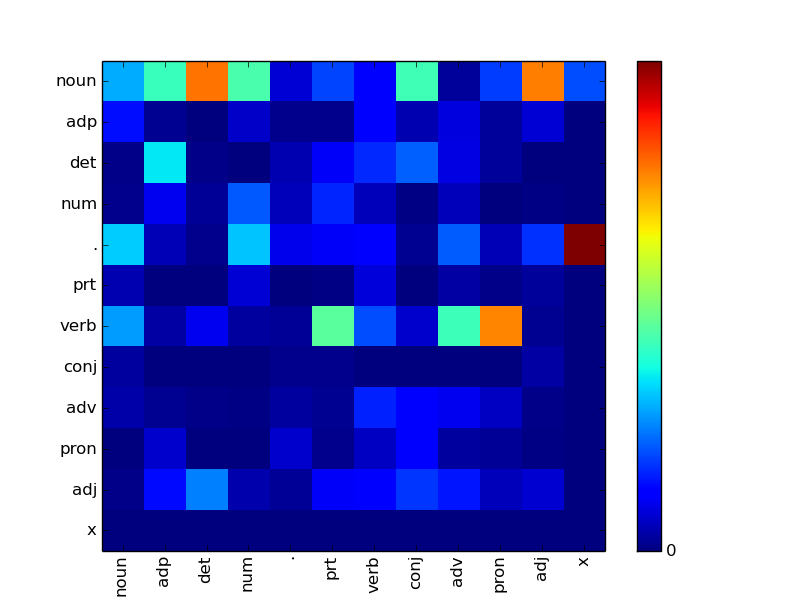
\includegraphics[scale=.5]{figs/sequences/transition_probs}
\caption{\label{fig:transProbs} Transition probabilities of the
trained model. Each column is previous state and row is current
state. Note the high probability of having Noun after Adjective, or of having Verb after Noun, as expected.}
\end{figure}

\begin{exercise}
Test the model using both posterior decoding and Viterbi decoding on
both the train and test set, using the methods in class HMM:
\begin{python}
>>> viterbi_pred_train = hmm.viterbi_decode_corpus(train_seq)
>>> posterior_pred_train = hmm.posterior_decode_corpus(train_seq)
>>> eval_viterbi_train =   hmm.evaluate_corpus(train_seq, viterbi_pred_train)
>>> eval_posterior_train =  hmm.evaluate_corpus(train_seq, posterior_pred_train)
>>> print "Train Set Accuracy: Posterior Decode \%.3f, Viterbi Decode: \%.3f"\%(eval_posterior_train,eval_viterbi_train)
Train Set Accuracy: Posterior Decode 0.985, Viterbi Decode: 0.985
>>> viterbi_pred_test = hmm.viterbi_decode_corpus(test_seq)
>>> posterior_pred_test = hmm.posterior_decode_corpus(test_seq)
>>> eval_viterbi_test =   hmm.evaluate_corpus(test_seq,viterbi_pred_test)
>>> eval_posterior_test = hmm.evaluate_corpus(test_seq,posterior_pred_test)
>>> print "Test Set Accuracy: Posterior Decode \%.3f, Viterbi Decode: \%.3f"\%(eval_posterior_test,eval_viterbi_test)
Test Set Accuracy: Posterior Decode 0.350, Viterbi Decode: 0.509
\end{python}

What do you observe? Remake the previous exercise but now train the HMM
using smoothing. Try different values (0,0.1,0.01,1) and report the results on the
train and development set. (Use function
\emph{pick\_best\_smoothing}).


\begin{python}
>>> best_smothing = hmm.pick_best_smoothing(train_seq, dev_seq, [10,1,0.1,0])
Smoothing 10.000000 --  Train Set Accuracy: Posterior Decode 0.731, Viterbi Decode: 0.691
Smoothing 10.000000 -- Test Set Accuracy: Posterior Decode 0.712, Viterbi Decode: 0.675
Smoothing 1.000000 --  Train Set Accuracy: Posterior Decode 0.887, Viterbi Decode: 0.865
Smoothing 1.000000 -- Test Set Accuracy: Posterior Decode 0.818, Viterbi Decode: 0.792
Smoothing 0.100000 --  Train Set Accuracy: Posterior Decode 0.968, Viterbi Decode: 0.965
Smoothing 0.100000 -- Test Set Accuracy: Posterior Decode 0.851, Viterbi Decode: 0.842
Smoothing 0.000000 --  Train Set Accuracy: Posterior Decode 0.985, Viterbi Decode: 0.985
Smoothing 0.000000 -- Test Set Accuracy: Posterior Decode 0.370, Viterbi Decode: 0.526
>>> hmm.train_supervised(train_seq, smoothing=best_smothing)
>>> viterbi_pred_test = hmm.viterbi_decode_corpus(test_seq)
>>> posterior_pred_test = hmm.posterior_decode_corpus(test_seq)
>>> eval_viterbi_test =   hmm.evaluate_corpus(test_seq, viterbi_pred_test)
>>> eval_posterior_test = hmm.evaluate_corpus(test_seq, posterior_pred_test)
>>> print "Best Smoothing \%f --  Test Set Accuracy: Posterior Decode \%.3f, Viterbi Decode: \%.3f"%(best_smothing,eval_posterior_test,eval_viterbi_test)
Best Smoothing 0.100000 --  Test Set Accuracy: Posterior Decode 0.837, Viterbi Decode: 0.827
\end{python}


Perform some error analysis to understand were the errors are coming
from. You can start by visualizing the confusion matrix (true tags vs
predicted tags). You should get something like \ref{fig:cm_uns}.

\begin{python}
>>> import sequences.confusion_matrix as cm
>>> confusion_matrix = cm.build_confusion_matrix(test_seq.seq_list, viterbi_pred_test, len(corpus.tag_dict), hmm.get_num_states())
>>> cm.plot_confusion_bar_graph(confusion_matrix, corpus.tag_dict, xrange(hmm.get_num_states()), 'Confusion matrix')
>>> plt.show()
\end{python}

\begin{figure}
\centering
\includegraphics[scale=.5]{figs/sequences/cm_sup.png}
\caption{\label{fig:cm_uns} Confusion Matrix for the previous
  example. Predict tags are columns and the true tags corresponds to
  the constituents of each column.}
\end{figure}

\end{exercise}


%\begin{exercise}
%Implement a function that produces the accuracy for rare words vs
%common words. Use you own definition of rare word.
%
%Can you come up with other error analysis methods? Which?
%
%\end{exercise}

%\begin{exercise}
%So far we have only worked with a limited dataset of 1000 words. Try increasing the number of sentences to 10000. What do you observe?
%\end{exercise}


%\section{Unsupervised Learning of HMMs}
%
%\afm{explain here the EM algorithm}
%
%\begin{python}
%
%Initial accuracy: 0.303638
%Iter: 1 Log Likelihood: -101824.763927
%Iter: 1 Accuracy: 0.305441
%Iter: 2 Log Likelihood: -78057.108346
%Iter: 2 Accuracy: 0.321976
%Iter: 3 Log Likelihood: -77813.725501
%Iter: 3 Accuracy: 0.357451
%Iter: 4 Log Likelihood: -77192.947674
%Iter: 4 Accuracy: 0.385109
%Iter: 5 Log Likelihood: -76191.800849
%Iter: 5 Accuracy: 0.392123
%Iter: 6 Log Likelihood: -75242.572729
%Iter: 6 Accuracy: 0.391121
%Iter: 7 Log Likelihood: -74392.892496
%Iter: 7 Accuracy: 0.404249
%Iter: 8 Log Likelihood: -73357.542833
%Iter: 8 Accuracy: 0.399940
%Iter: 9 Log Likelihood: -72135.182778
%Iter: 9 Accuracy: 0.399238
%Iter: 10 Log Likelihood: -70924.246230
%Iter: 10 Accuracy: 0.395430
%Iter: 11 Log Likelihood: -69906.561800
%Iter: 11 Accuracy: 0.394328
%Iter: 12 Log Likelihood: -69140.228623
%Iter: 12 Accuracy: 0.390821
%Iter: 13 Log Likelihood: -68541.416423
%Iter: 13 Accuracy: 0.391522
%Iter: 14 Log Likelihood: -68053.456865
%Iter: 14 Accuracy: 0.389117
%Iter: 15 Log Likelihood: -67667.318961
%Iter: 15 Accuracy: 0.386411
%Iter: 16 Log Likelihood: -67337.685686
%Iter: 16 Accuracy: 0.385409
%Iter: 17 Log Likelihood: -67054.571821
%Iter: 17 Accuracy: 0.385409
%Iter: 18 Log Likelihood: -66769.973881
%Iter: 18 Accuracy: 0.385409
%Iter: 19 Log Likelihood: -66442.608458
%Iter: 19 Accuracy: 0.385409
%
%\end{python}


\section{\label{unsupervised} Unsupervised Learning of HMMs}
We next address the problem of \emph{unsupervised} learning. 
In this setting, we are not given any labeled data; all we get to see is a set of natural language sentences.  
The underlying question is: 
\begin{quote}
Can we learn something from raw text?
\end{quote}
This task is challenging, since the process by which linguistic structures are generated is not always clear; 
and even when it is, it is typically too complex to be
formally expressed. Nevertheless, unsupervised learning has been applied to a
wide range of NLP tasks, such as: 
\pos\ Induction  \citep{schutze1995distributional,merialdo1994tet,clark03combining},
Dependency Grammar Induction \citep{klein2004acl,smith2006annealing}, Constituency Grammar Induction \citep{klein2004acl}, Statistical Word Alignments 
\citep{brown94mathematic} and Anaphora Resolution \citep{charniak2009works}, just to name a few. 

Different motivations have pushed research in this area. From both a linguistic and cognitive point of view, 
unsupervised learning is useful as a tool to study language acquisition. 
From a machine learning point of view, unsupervised learning is a fertile ground for testing new learning methods, 
where significant improvements can yet be made. 
From a more pragmatic perspective, unsupervised learning is required
since annotated corpora is a scarce resource for different reasons. Independently of the reason, unsupervised learning is an increasing active field of research.

A first problem with unsupervised learning, since we don't observe any labeled data (i.e., 
the training set is now $\mathcal{D}_{U} = \{x^1,\ldots, x^M\}$), 
is that most of the methods studied so far (e.g., Perceptron, MIRA, SVMs) cannot be used since we cannot compare 
the true output with the predicted output. 
Note also that a direct minimization of the \emph{complete negative log-likelihood} of the data, $\log P_{\theta}(X^1=x^1,\ldots,X^M=x^m)$, 
is very challenging, since it would require marginalizing out (\emph{i.e.}, summing over) all possible hidden variables:
\begin{equation}
 \log P_{\theta}(X^1=x^1,\ldots,X^M=x^m) =  \sum_{m=1}^M \log \sum_{y \in \Lambda} P_{\theta} (X=x^m,Y=y).
\end{equation}
Note also that the objective above is \emph{non-convex} even for a linear model: hence, it may have local minima, which makes optimization much 
more difficult.%
%\footnote{Another observation is that normally we are restricted to generative models, 
%with some remarkable exceptions~\citep{smith2005acl}, since the objective of discriminative models when no labels are observed are 
%meaningless ($\sum_{y^m } P(y^m |x^m) = 1$); this rules out, for instance, Maximum Entropy classifiers.}

The most common optimization method in the presence of hidden (latent) variables is the Expectation Maximization (EM) algorithm, described in the next section. Note that this algorithm is a generic optimization routine that does not depend on a particular model. Later, in Section \ref{posi} we will apply the EM algorithm to the task of part-of-speech induction, where one is given raw text and a number of clusters and the task is to cluster words that behave similarly in a grammatical sense. 

\subsection{\label{em}Expectation Maximization Algorithm}
Given the training corpus $\mathcal{D}_{U} := \{x^1, \ldots, x^M\}$, training 
seeks model parameters $\theta$ that minimize the negative log-likelihood of the corpus:
\begin{equation}
\label{loglikelihoood}
\mathbf{Negative\;Log\;Likelihood\!:}\;\;\;\; \likelihood(\theta) = \widehat{\mathbb{E}} [-\log P_{\theta}(X)] = -\frac{1}{M}\sum_{m=1}^M \log \left( \sum_{y^m \in \Lambda} P_{\theta}(X=x^m,Y=y^m) \right),
\end{equation}
where $\widehat{\mathbb{E}}[f(X)] := \frac{1}{M}\sum_{m=1}^{M} f(x^m)$ denotes the empirical average of a function $f$ over the training corpus. Because of the hidden variables $y^1,\ldots,y^M$, the likelihood term contains a
sum over all possible hidden structures inside of a logarithm, which
makes this quantity hard to compute.

The most common minimization
algorithm to fit the model parameters in the presence of hidden
variables is the Expectation-Maximization (EM) algorithm. 
The EM procedure can be thought of intuitively in the following way. 
If we observe the hidden variables' values for all sentences in the
corpus, then we could easily compute the maximum likelihood value of
the parameters as described in Section \ref{ml}. 
On the other hand, if we had the model parameters we could label data
using the model, and collect the
sufficient statistics described in Section \ref{ml}.
However, since we are working in an unsupervised setting, we never get to
observe the hidden state sequence. Instead, given the 
training set $\mathcal{D}_{U} = \{x^1 \ldots x^M\}$, we will need to
collect \emph{expected} sufficient statistics (in this case, \emph{expected} counts) 
that
represent the number of times that each hidden variable is
expected to be used with the current parameters setting. These expected sufficient
statistics will then be used during learning as ``fake'' observations of
the hidden variables. Using the node and edge posterior distributions
described in Equations \ref{eq::nodePosterior} and \ref{eq::edgePosterior},
the expected sufficient statistics can 
be computed by the following formulas:

\begin{align}
\mathbf{Initial \ Counts\!:}\;\;\;\;  &  C_{\mathrm{init}}(c_k) = \sum_{m=1}^M
P_{\theta} (Y^m_1 = c_k \,\,|\,\, X^m = x^m); \label{eq::initialCountsPost}\\
%
%\mathbf{Final \ Counts\!:}\;\;\;\;  &  fc(\hv_l,\hv _m) = \sum_{\trex} 
%\Ind (\hs_N = \hv_l \mid \hs_{N-1} = \hv_m); \label{eq::finalCounts}\\
%
\mathbf{Transition \ Counts\!:}\;\;\;\;  &  C_{\mathrm{trans}}(c_k,c_l) =
\sum_{m=1}^M  \sum_{i = 2}^{N}
P_{\theta}(Y^m_i = c_k \wedge Y^m_{i-1} = c_l \,\,|\,\, X^m = x^m); \label{eq::transitionCountsPost}\\
%
\mathbf{Final \ Counts\!:}\;\;\;\;  &  C_{\mathrm{final}}(c_k) = \sum_{m=1}^M
P_{\theta} (Y^m_N = c_k \,\,|\,\, X^m = x^m); \label{eq::finalCountsPost}\\
%
\mathbf{Emission \ Counts\!:}\;\;\;\;  &  
C_{\mathrm{emiss}}(w_j,c_k) = \sum_{m=1}^M
\sum_{i = 1}^{N}
\Ind (x^m_i = w_j) P_{\theta}(Y^m_i = c_k \,\,|\,\, X^m = x^m); \label{eq::emissionCountsPost}
\end{align}

%\begin{align}
%\mathbf{Initial \ Counts\!:}\;\;\;\;  &  ic(\hv_l) = \sum_{d=1}^D
%\gamma_1 (\hv_l); \label{eq::initialCountsPost}\\
%\mathbf{Final \ Counts\!:}\;\;\;\;  &  fc(\hv_N,\hv _{N-1}) = \sum_{d=1}^D  \xi_{N-1} (\hv_l,\hv_m); \label{eq::finalCountsPost}\\
%\mathbf{Transition \ Counts\!:}\;\;\;\;  &  tc(\hv_l,\hv _m) = \sum_{d=1}^D \sum_{i = 1}^{N-1}  \xi_i (\hv_l,\hv_m); \label{eq::transitionCountsPost}\\
%\mathbf{State \ Counts\!:}\;\;\;\;  &  sc(\vv_q,\hv_m) = \sum_{d=1}^D \sum_{i = 1 , \obs_i = \vv_q }^{N}  \gamma_i (\hv_m). \label{eq::stateCountsPost}
%\end{align}

Compare the previous equations with the ones described in Section
\ref{ml} for the same quantities (Eqs.~\ref{eq::initialCounts}--\ref{eq::emissionCounts}). The main difference is that while in
the presence of supervised data you sum the observed events, when you
have no label data you sum the posterior probabilities of each
event. If these probabilities were such that the probability mass was
around single events then both equations will produce the same result.



The EM procedure starts with an initial guess for the parameters
$\theta^0$ at time $t = 0$. The algorithm keeps iterating 
until it converges to a local minima of the negative log likelihood. Each
iteration is divided into two steps:
\begin{itemize} 
 \item The {\bf{E-Step}} (Expectation) 
computes the posteriors for the hidden variables $P_{\theta^t}(Y|X=x^m)$
given the current parameter values $\theta^t$ and the observed variables $X=x^m$ for the $m$-th sentence. 
For an HMM, this can be done through the Forward-Backward algorithm described in the previous sections.
\item The {\bf{M-step}} (Maximization) uses those posteriors $P_{\theta^t}(Y|X=x^m)$ to
``softly fill in'' the values of the hidden variables $Y^m$, and
collects the sufficient statistics: initial counts (Eq: \ref{eq::initialCountsPost}), transition counts (Eq:
\ref{eq::transitionCountsPost}), 
final counts  (Eq: \ref{eq::finalCountsPost}),
and emission counts (Eq: \ref{eq::emissionCountsPost}). These
counts are then used to estimate maximum likelihood parameters $\theta^{t+1}$, as described in
Section \ref{ml}.
\end{itemize}

The EM algorithm is guaranteed to
converge to a local minimum of the negative log-likelihood $\likelihood(\theta)$, under mild
conditions.  
Note that we are not committing to the best assignment of the hidden variables, but
summing the occurrences of each parameter weighed by the posterior
probability of all possible assignments. 
This modular split into two intuitive and straightforward steps
accounts for the vast popularity of EM.%
\footnote{More formally, EM minimizes an \emph{upper bound} of $\likelihood(\theta)$ via block-coordinate descent. See \citet{Neal1998} for details. Also, even though we are presenting EM in the context of HMMs, this algorithm can be more broadly applied to any probabilistic model with latent variables.} %

% on an upper bound $F(q,\theta)$ using an auxiliary distribution over the latent variables
%$\auxq$:
%\begin{eqnarray}
%\likelihood(\theta)  &=& \XpD \left[-\log \sum_{\hseq}\joint \right]\\
%\label{eq:jensen}&=& \XpD \left[-\log \sum_{\hseq}
%\auxq*\frac{\joint}{\auxq}\right] \le \XpD \left[- \sum_{\hseq} \auxq\log \frac{\joint}{\auxq}\right] \\
%&=& \XpD \left[\sum_{\hseq} \auxq\log \frac{\auxq}{\joint}\right] =  F(q,\theta),
%\end{eqnarray}
%where we have multiplied and divided the $\joint$ by the same quantity
%$\auxq$, and 
%the lower bound comes from applying Jensen Inequality (Equation
%\ref{eq:jensen}). $F(q,\theta)$ is normally referred to as the energy
%function, which comes from the physics field and refers to the energy of a given system that we want to minimize.
%\begin{equation}
%\mathbf{EM\;Upper\;Bound\!:}\;\;\;\;\;\likelihood(\theta) \le F(q,\theta) =
%\XpD \left[\sum_{\hseq} \auxq\log \frac{\auxq}{\joint}\right].
%\end{equation}
%The alternating E and M steps at iteration $t+1$ can be seen as minimizing the energy function first 
%with respect to $\auxq$ and then with respect to $\theta$:
%\begin{eqnarray}
%\hspace{-5mm}{\mathbf E\!:}&& q^{t+1}(\hseq\mid\sent) =
%\argmin_{\auxq} F(q,\theta^t)
%  = \argmin_{\auxq} \KL(q(\hseq\mid\sent)\,||\,p_{\theta^t}(\hseq\mid\sent)) = p_{\theta^t}(\hseq\mid\sent);
% \label{eq:e-step} \\
%\hspace{-5mm}{\mathbf M\!:}&& \theta^{t+1} = \argmin_\theta
%F(q^{t+1},\theta) = \argmax_\theta \XpD\!\left[\sum_{\hseq}
%q^{t+1}(\hseq\mid\sent)\log p_\theta(\sent,\hseq)\right];
%\label{eq:m-step}
%\end{eqnarray}
%where $\KL(q||p) = \Xp_q[\log \frac{q(\cdot)}{p(\cdot)}]$ is the
%Kullback-Leibler divergence. The KL term in the E-Step results from 
%dropping all terms from the energy function that are constant for a
%set $\theta$, in this case the likelihood of the observation sequence
%$\marginal$:
%
%\begin{align}
%\sum_{\hseq} \auxq\log \frac{\auxq}{\joint} &= \sum_{\hseq} \auxq\log
%\auxq - \sum_{\hseq} \auxq\log \joint  \\ 
%&= \sum_{\hseq} \auxq\log \auxq - \sum_{\hseq} \auxq\log \marginal
%\posterior \\
%&= \sum_{\hseq} \auxq\log \frac{\auxq}{\posterior} - \log \marginal \\
%&= \KL(\auxq||\posterior) - \log \marginal.
%\end{align}

Algorithm ~\ref{alg::em} presents the pseudo code for the EM
algorithm. 
%Note that this algorithm is agnostic of a particular model,
%it only requires the model to implement a common interface.

\begin{algorithm}
\begin{algorithmic}[1]
  \STATE {\bfseries input:} dataset $\mathcal{D}_{U}$, initial model $\theta$
    \FOR{$t = 1$ {\bfseries to} $T$}
    	  \STATE
    	  \STATE \textbf{E-Step:}
      \STATE Clear counts: $C_{\mathrm{init}}(.) = C_{\mathrm{trans}}(.,.) = C_{\mathrm{final}}(.) = C_{\mathrm{emiss}}(.,.) = 0$
      \FOR{$x^m \in \mathcal{D}_{U}$}
      	\STATE Compute posterior expectations $P_{\theta}(Y_i|X=x^m)$ and $P_{\theta}(Y_i,Y_{i+1}|X=x^m)$ using the current model $\theta$
%        \STATE posteriors,likelihood =model.compute\_posteriors($seq$)
%        \STATE model.update\_counts($seq$,posteriors)
      \STATE Update counts as shown in Eqs.~\ref{eq::initialCountsPost}--\ref{eq::emissionCountsPost}.
      \ENDFOR
    	  \STATE
      \STATE \textbf{M-Step:}
         \STATE Update the model parameters $\theta$ based on the counts.
    \ENDFOR
\end{algorithmic}    
\caption[EM algorithm]{\label{alg::em}  EM algorithm.} 
\end{algorithm}


One important thing to note in Algorithm \ref{alg::em} is that for the
HMM model we already have all the model pieces we require. In fact
the only method we don't have yet implemented from previous classes is
the method to update the counts given the posteriors. 

\begin{exercise}

Implement the method to update the counts given the state and transition posteriors.
\begin{python}
 def update_counts(self, sequence, state_posteriors, transition_posteriors):
\end{python}

%Use the method you defined previously to check the count tables to
%check if this method is correct. Use a corpus with only one sentence
%to make the test simpler.

%\begin{python}
%In []: run readers/pos_corpus.py
%In []: posc = PostagCorpus("en",max_sent_len=15,train_sents=1,dev_sents=0,test_sents=0)
%In []: run sequences/hmm.py
%In []: hmm = HMM(posc)
%In []: hmm.train_supervised(posc.train,smoothing=0.1)
%In []: hmm.clear_counts()
%In []: posteriors,likelihood = hmm.get_posteriors(posc.train.seq_list[0])
%In []: hmm.update_counts(posc.train.seq_list[0],posteriors)
%In []: hmm.sanity_check_counts(posc.train)
%\end{python}

%If you pass this test, then you have all the pieces to implement the
%EM algorithm. Look at the code for EM algorithm in file
%\emph{sequences/em.py} and check it for yourself. 

You now have all the pieces to implement the
EM algorithm. Look at the code for EM algorithm in file
\emph{sequences/hmm.py} and check it for yourself. 

\begin{python}
    def train_EM(self, dataset, smoothing=0, num_epochs=10, evaluate=True):
        self.initialize_random()

        if evaluate:
            acc = self.evaluate_EM(dataset)
            print "Initial accuracy: %f"%(acc)
            
        for t in xrange(1, num_epochs):
            #E-Step
            total_log_likelihood = 0.0
            self.clear_counts(smoothing)
            for sequence in dataset.seq_list:
                # Compute scores given the observation sequence.
                initial_scores, transition_scores, final_scores, emission_scores = \
                    self.compute_scores(sequence)
                
                state_posteriors, transition_posteriors, log_likelihood = \
                    self.compute_posteriors(initial_scores,
                                            transition_scores,
                                            final_scores,
                                            emission_scores)

                self.update_counts(sequence, state_posteriors, transition_posteriors)
                total_log_likelihood += log_likelihood
            print "Iter: %i Log Likelihood: %f"%(t, total_log_likelihood)
            #M-Step
            self.compute_parameters()
            if evaluate:
                 ### Evaluate accuracy at this iteration
                acc = self.evaluate_EM(dataset)
                print "Iter: %i Accuracy: %f"%(t,acc)
\end{python}

\end{exercise}

%%% Local Variables: 
%%% mode: latex
%%% TeX-master: "../../guide"
%%% End: 




\subsection{\label{posi}Part of Speech Induction}
In this section we present the \posi\ task. \pos\ tags are pre-requisite for many text applications. The task of \pos\ tagging where one is given a labeled training set of words and respective tags is a well studied task with several methods achieving high prediction quality, as we saw in the first part of this chapter. %Chapters \ref{day:seq} and \ref{day:seq_disc}. 

On the other hand the task of \posi\ where one does not have access to a labeled corpus is a much harder task with a huge space for improvement. In this case, we are given only the raw text along with sentence boundaries and a predefined number of clusters we can use. This problem can be seen as a clustering problem. We want to cluster words that behave grammatically in the same way on the same cluster. This is a much harder problem.

%Formally, the problem setting is the following: we are given a training set $\X = \sent^1 \ldots \sent^D$ of $D$ training examples, where each example $\sent = \obs_1 \ldots \obs_N$ is a sentence of $N$ words, whose values $\vv$ are taken from a vocabulary $\vocab$ of possible word types. We are also given the set of clusters $\hvocab$ that we are allowed to use. The hidden structure $\hseq = \hs_1 \ldots \hs_N$ corresponds to a sequence of cluster assignments for each individual word, such that $\hs_n = \hv_l$ with $\hv_l \in \hvocab$. 
%
Depending on the task at hand we can pick an arbitrary number of clusters. If the goal is to test how well our method can recover the true POS tags then we should use the same number of clusters as POS tags. On the other hand, if the task is to extract features to be used by other methods we can use a much bigger number of clusters (e.g., 200) to capture correlations not captured by POS tags, like lexical affinity. 

Note, however that nothing is said about the identity of each cluster. The model has no preference in assigning cluster 1 to nouns vs cluster 2 to nouns. Given this non-identifiability several metrics have been proposed for evaluation \citep{Reichart09,haghighi2006naacl,Meila07,RosenbergH07}. In this class we will use a common and simple metric called \textbf{1-Many}, which maps each cluster to majority pos tag that it contains (see Figure \ref{fig:cm_uns} for an example). 

\begin{figure}
\centering
\includegraphics[scale=.5]{figs/sequences/cm_uns1.png}
\caption{\label{fig:cm_uns} Confusion Matrix example. Each cluster is a column. The best tag in each column is represented under the column (1-many) mapping. Each color represents a true Pos Tag.}
\end{figure}


\begin{exercise}
Run 20 epochs of the EM algorithm for part of speech induction:
\begin{python}
>>> hmm.train_EM(train_seq, 0.1, 20, evaluate=True)
>>> viterbi_pred_test = hmm.viterbi_decode_corpus(test_seq)
>>> posterior_pred_test = hmm.posterior_decode_corpus(test_seq)
>>> eval_viterbi_test =   hmm.evaluate_corpus(test_seq, viterbi_pred_test)
>>> eval_posterior_test = hmm.evaluate_corpus(test_seq, posterior_pred_test)

Initial accuracy: 0.303638
Iter: 1 Log Likelihood: -101824.763927
Iter: 1 Accuracy: 0.305441
Iter: 2 Log Likelihood: -78057.108346
Iter: 2 Accuracy: 0.321976
Iter: 3 Log Likelihood: -77813.725501
Iter: 3 Accuracy: 0.357451
Iter: 4 Log Likelihood: -77192.947674
Iter: 4 Accuracy: 0.385109
Iter: 5 Log Likelihood: -76191.800849
Iter: 5 Accuracy: 0.392123
Iter: 6 Log Likelihood: -75242.572729
Iter: 6 Accuracy: 0.391121
Iter: 7 Log Likelihood: -74392.892496
Iter: 7 Accuracy: 0.404249
Iter: 8 Log Likelihood: -73357.542833
Iter: 8 Accuracy: 0.399940
Iter: 9 Log Likelihood: -72135.182778
Iter: 9 Accuracy: 0.399238
Iter: 10 Log Likelihood: -70924.246230
Iter: 10 Accuracy: 0.395430
Iter: 11 Log Likelihood: -69906.561800
Iter: 11 Accuracy: 0.394328
Iter: 12 Log Likelihood: -69140.228623
Iter: 12 Accuracy: 0.390821
Iter: 13 Log Likelihood: -68541.416423
Iter: 13 Accuracy: 0.391522
Iter: 14 Log Likelihood: -68053.456865
Iter: 14 Accuracy: 0.389117
Iter: 15 Log Likelihood: -67667.318961
Iter: 15 Accuracy: 0.386411
Iter: 16 Log Likelihood: -67337.685686
Iter: 16 Accuracy: 0.385409
Iter: 17 Log Likelihood: -67054.571821
Iter: 17 Accuracy: 0.385409
Iter: 18 Log Likelihood: -66769.973881
Iter: 18 Accuracy: 0.385409
Iter: 19 Log Likelihood: -66442.608458
Iter: 19 Accuracy: 0.385409

>>> confusion_matrix = cm.build_confusion_matrix(test_seq.seq_list, viterbi_pred_test, 
                                             len(corpus.tag_dict), hmm.get_num_states())
>>> cm.plot_confusion_bar_graph(confusion_matrix, corpus.tag_dict, 
                            xrange(hmm.get_num_states()), 'Confusion matrix')
\end{python}
Note: your results may not be the same as in this example since we are using a random start, but the trend should be the same, with likelihood decreasing at every iteration (\terxtbf{the values in the example are the log likelihood, or the negative log likelihhod? if it is the fisrt, it is actually increasing}). 
%Also note that in some iterations the likelihood does not go down because of some rounding errors, however the general trend is that likelihood decreases over iterations. 
\end{exercise}

In the previous exercise we used an HMM to do Part-of-Speech induction using 12 clusters (by omission the HMM uses as number of hidden states the one provided by the corpus). A first observation is that the log-likelihood is always increasing as expected. Another observation is that the accuracy goes up from 33\% to 41\%. Note that normally you will run this algorithm for 200 iterations, we stopped earlier for time constraints. Another observations is that the accuracy is not monotonic increasing, this is because the likelihood is not a perfect proxy for the accuracy. In fact all that likelihood is measuring are co-occurrences of words in the corpus; it has no idea of pos tags. The fact we are improving derives from the fact that language is not random but follows some specific hidden patterns. In fact this patterns are what true pos-tags try to capture. A final observation is that the performance is really bad compared to the supervised scenario, so there is a lot of space for improvement. The actual state of the art is around 71\% for fully unsupervised~\citep{JoaoThesis,bergkirkpatrick2010naacl} and 80\% \citep{das-petrov:2011:ACL-HLT2011} using parallel data and information from labels in the other language. 

Looking at Figure \ref{fig:cm_uns} shows the confusion matrix for this particular example. 
A first observation is that most clusters are mapped to nouns, verbs or punctuation. 
This is a known fact since there are many more nouns and verbs than any other tags. Since maximum likelihood prefers probabilities 
to be uniform (imagine two parameters: in one setting both have value 0.5 so the likelihood will be 0.5*0.5 = 0.25, 
while in the other case one as 0.1 and 0.9 so the maximum likelihood is 0.09). Several approaches have been proposed to 
address this problem, moving towards a Bayesian setting \citep{johnson2007dtf}, or using 
Posterior Regularization \citep{graca2009nips}. 
%more about this later today. 
%Part-of-Speech induction is a very active field of research, in fact in the last two ACL conferences (Association for Computational Linguistics) the short paper award (2010) and the best paper award (2011) were about this topic~\citep{lamar-EtAl:2010:Short,das-petrov:2011:ACL-HLT2011}.








% \begin{exercise}

% Repeat the previous exercise using a different number of hidden states (20,50). Note that the higher the number of states is the slower the training will be.
% What do you observe? Look at the confusion matrix and try to explaing what is happening.

% \begin{python}
% In []: run readers/pos_corpus.py
% In []: posc = PostagCorpus("en",max_sent_len=15,train_sents=1000,dev_sents=0,test_sents=0)
% In []: run sequences/hmm.py
% In []: hmm = HMM(posc,nr_states=20)
% In []: hmm.initialize_radom()
% In []: run sequences/em.py
% In []: em = EM(posc,hmm)
% In []: em.train(posc.train,nr_iter=20)
% Init acc 0.348933
% Iter: 1 Negative Log Likelihood 16.038424
% Iter: 1 acc 0.362662
% Iter: 2 Negative Log Likelihood 11.200816
% Iter: 2 acc 0.370177
% Iter: 3 Negative Log Likelihood 11.046597
% Iter: 3 acc 0.380800
% Iter: 4 Negative Log Likelihood 10.607496
% Iter: 4 acc 0.389518
% Iter: 5 Negative Log Likelihood 9.809817
% Iter: 5 acc 0.394027
% Iter: 6 Negative Log Likelihood 8.949717
% Iter: 6 acc 0.396733
% Iter: 7 Negative Log Likelihood 8.105404
% Iter: 7 acc 0.398337
% Iter: 8 Negative Log Likelihood 7.366612
% Iter: 8 acc 0.392925
% Iter: 9 Negative Log Likelihood 7.005009
% Iter: 9 acc 0.393126
% Iter: 10 Negative Log Likelihood 6.895723
% Iter: 10 acc 0.397034
% Iter: 11 Negative Log Likelihood 6.851836
% Iter: 11 acc 0.397134
% Iter: 12 Negative Log Likelihood 6.818365
% Iter: 12 acc 0.399238
% Iter: 13 Negative Log Likelihood 6.782213
% Iter: 13 acc 0.406053
% Iter: 14 Negative Log Likelihood 6.755121
% Iter: 15 Negative Log Likelihood 6.745873
% Iter: 15 acc 0.419681
% Iter: 16 Negative Log Likelihood 6.743681
% Iter: 16 acc 0.424291
% Iter: 17 Negative Log Likelihood 6.745030
% Iter: 17 acc 0.431406
% Iter: 18 Negative Log Likelihood 6.747628
% Iter: 18 acc 0.434512
% Iter: 19 Negative Log Likelihood 6.749084
% Iter: 19 acc 0.438721
% pred = hmm.viterbi_decode_corpus(posc.train.seq_list)
% cm = build_confusion_matrix(posc.train.seq_list,pred,len(posc.int_to_pos),hmm.nr_states)
% plot_confusion_bar_graph(cm,posc.int_to_pos,range(12),"test")
% \end{python}

% \end{exercise}

%%% Local Variables: 
%%% mode: latex
%%% TeX-master: "../../guide"
%%% End: 




%%% Local Variables: 
%%% mode: latex
%%% TeX-master: "../../guide"
%%% End: 





%\section{\label{hmm_special_state} HMM Initial and Final State}
%\input{pages/sequences/init_final_hmm.tex}

%\section{\label{hmm} Second order HMM}
%\input{pages/sequences/second_order_hmm.tex}


%%% Local Variables: 
%%% mode: latex
%%% TeX-master: "../../guide.tex"
%%% End: 


\chapter{Transformers}
\let\thefootnote\relax\footnotetext{Authors in alphabetical order: Goncalo Melo, Grig Vardayan, Hovhanes Tamoyan, Israfel Salazar, Li Haau-Sing, Roberto Dessi, Venelin Kovachev
}
\section{Today's assignment}
Today's class will demystify the Transformer architecture \cite{vaswani2017attention}. Transformers have become the dominant model in Natural Language Processing pushing the performance of all tasks through models like BERT \cite{devlin2018bert} and GPT \cite{brown2020language}. In this class, we will review the architecture of Transformers. The focus of the class is to understand and implement the self-attention mechanism in Pytorch. For this, we will use an annotated version of Karpathy's minGPT code (\url{https://github.com/karpathy/minGPT}).


\section{Before Diving into Transformers}
Before diving into transformers, we would like to introduce two important pieces of details to defining and training transformers.


\subsection{Positional Encoding}
Different from models with recurrence/convolution, positional information is not encoded in Transformers. Therefore, \citet{vaswani2017attention} include the positional embedding as part of the input to Transformers. The most popular way to compute the positional embedding ($PE$) is to use the sinusoidal expressed as
\begin{equation}
        PE_{(pos,2i)} = \mathrm{sin}\left(\frac{pos}{ 10000^{2i/d_{model}}}\right),
\end{equation}
\begin{equation}
    PE_{(pos,2i+1)} = \mathrm{cos}\left(\frac{pos}{ 10000^{2i/d_{model}}}\right),
\end{equation}

where $pos$ is the position and $i$ is the dimension.

\subsection{Tokenization}
To break down a given input string into atomic pieces, the tokenization operation is performed. There are various techniques available for applying tokenization, with word-based and character-level tokenization being the two extremes. Each approach has its advantages and considerations for specific cases. The subword tokenization strikes a balance between these two approaches.

Subword tokenization operates on the idea that frequently occurring words should be included in the vocabulary, while rare words should be split into more common subwords. This approach aims to handle a wider range of word types effectively.

Transformers utilize the byte pair encoding (BPE) approach \citep{bpe} during training. BPE enables the encoding of rare and unknown words as sequences of subword units, contributing to the overall flexibility and performance of the model.

\begin{exercise}
Tokenization

Let's see how the three mostly used tokenization techniques can be applied in practice.
\begin{enumerate}
\item Run the word-based tokenizer and try out different {\tt text}:
\begin{python}
text = "I travelled to Lisbon in July to attend an NLP summer school"
text.split()
\end{python}
\item Run the character-based tokenizer, try out different different {\tt text} and answer the corresponding question:
\begin{python}
text = "I will travel to Lisbon in July..."
tokenized = [c for c in text if c not in [",", ";", ":", "'", "!", "?"]]
print(tokenized)
\end{python}
Question: What other problems are character-based tokenizers posing to NLP models?


\item Run the BPE (byte-pair encoding) tokenizer, and answer the corresponding questions:
\begin{python}
import numpy as np
from lxmls.transformers.bpe import BPETokenizer

tokenizer = BPETokenizer()

sentence = "Your drawing is charmingly anachronistic."
tokenizer.encoder.encode_and_show_work(sentence)
\end{python}
Question: Do you have a guess on which word will be split subwords and which one won't?
\end{enumerate}
\end{exercise}



\section{Transformer Architectures}

The basic building block of the Transformer combines a large Feed forward network with a multi-head self-attention layer. We have seen feed forwards in previous days and we will focus here on multi-head self-attention. Refer to previous days for details on the basics of feed-forwards.

Transformer blocks can be found in three types: Encoder, Decoder, and Encoder-Decoder 

\begin{enumerate}
\item Encoders: map a sequence of $T$ observations, e.g. some word or sub-word units $x_1 \cdots x_T$ to a hidden representation of size $H$, yielding a matrix of embeddings of size $(H, T)$. These contextual embeddings can be used to build other models on top by adding extra layers e.g. BERT.
\item Decoders: given a sequence of $t$ observations, e.g. some word or sub-word units $x_{<t} = x_1 \cdots x_{t-1}$ provide a hidden representation for element $x_t$. This can be used to predict the next word given some partial sentence e.g. as in GPT. 
\item Cross-Attention-Decoders: map a sequence $x$ to another of different size $y$. For this, they first Encode $x$ using an encoder. And then use a modified Decoder, that uses an additional attention mechanism read the Encoder values to generate embeddings for $y_t$ given $y_{<t}$ and the $\mathrm{Encoder}(x)$. The original Transformer used for machine translation is the best example.
\end{enumerate}

Though with very different roles the three architectures are very close to each other and imply only minor modifications. We will focus here on the Encoder architecture first, and then we will explain the other two.

\section{Attention}
In this section, we will delve into the intricacies of the attention mechanism, aiming to grasp its underlying intuition and motivation. We will embark on a comprehensive exploration of its inner workings, unraveling its secrets along the way.

Attention mechanisms have become a crucial component in effective sequence modeling across different tasks e.g. Neural Machine Translation (NMT) \cite{vaswani2017attention}. They enable modeling relationships between elements in input or output sequences, regardless of their positional distance. \cite{bahdanau2014neural, kim2017structured}.

The state-of-the-art sequence modeling architectures that predate Transformers, such as Recurrent Neural Networks (RNN), have traditionally treated input information in a uniform manner. This means that no specific connections are established among the individual tokens to fully capture the intricate relationships between them. Essentially, each token denoted as $t_i$, receives information from all preceding tokens $t_1...t_{i-1}$ in a uniform fashion. However, as the value of $i$ increases, this approach often leads to information loss, as well as issues related to vanishing or exploding gradients \cite{hochreiter1997long}, due to the fixed dimensionality of the encoded information.

In order to mitigate the latter challenge, Long Short-Term Memory (LSTM) models were introduced. These models proposed mechanisms to manipulate the flow of information across states by selectively adding or removing pertinent and extraneous information \cite{hochreiter1997long}. By incorporating these mechanisms, LSTM models aimed to address the aforementioned issues and enhance the handling of information within the sequence.
The LSTM has demonstrated exceptional performance on challenging sequence prediction tasks, such as text translation, and swiftly emerged as the prevailing approach in the field \cite{cho2014learning, sutskever2014sequence}.

However, the issue of having a fixed-length internal representation persists, and to overcome this limitation in the encoder-decoder architecture, the Attention mechanism was introduced. The Attention mechanism offers various variants, and in this context, we will delve into the "Scaled Dot-Product Attention" as outlined in \cite{vaswani2017attention}.

To provide a practical demonstration of the complex relationships that the model needs to learn, let's consider the following example: \emph{``The cat didn't climb the tree because it was too scared.``}.
\begin{figure}[h]
    \centering
    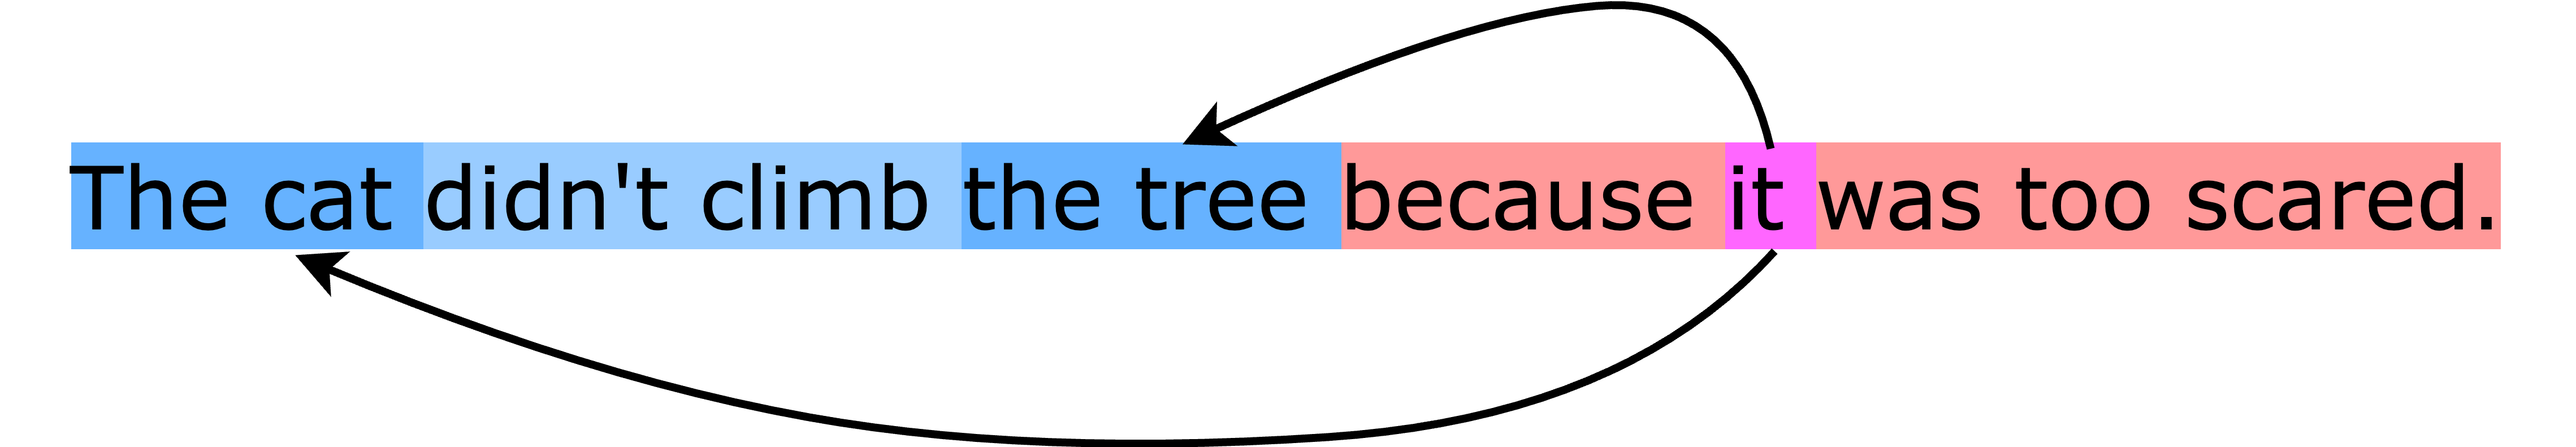
\includegraphics[width=8cm]{pages/imgs/example.png}
    \caption{An example illustration}
    \label{fig:example}
\end{figure}
In the initial part of the example, the inner connections are relatively straightforward. However, in the subsequent segment starting from the word "because," the relationships become more intricate.
For a human being, the question of whether the pronoun "it" refers to the cat or the tree is relatively simple due to our prior knowledge about cats and trees. With our understanding of these concepts, we can confidently determine the intended reference of the word "it." 
However, for a model, discerning the referent of the pronoun "it" -- whether it pertains to the cat or the tree -- is not as straightforward. Therefore, we require a mechanism that does not treat all words with equal importance but rather allocates focus to different tokens.

This intuitive mechanism is known as Attention, which assigns significance to specific tokens for a selected token. In Figure \ref{fig:att_self_sample}, the attention mapping of our example is demonstrated. This is commonly referred to as Self-Attention, as the connections are attained at the internal level, i.e. between input tokens.

\begin{figure}[h]
    \centering
    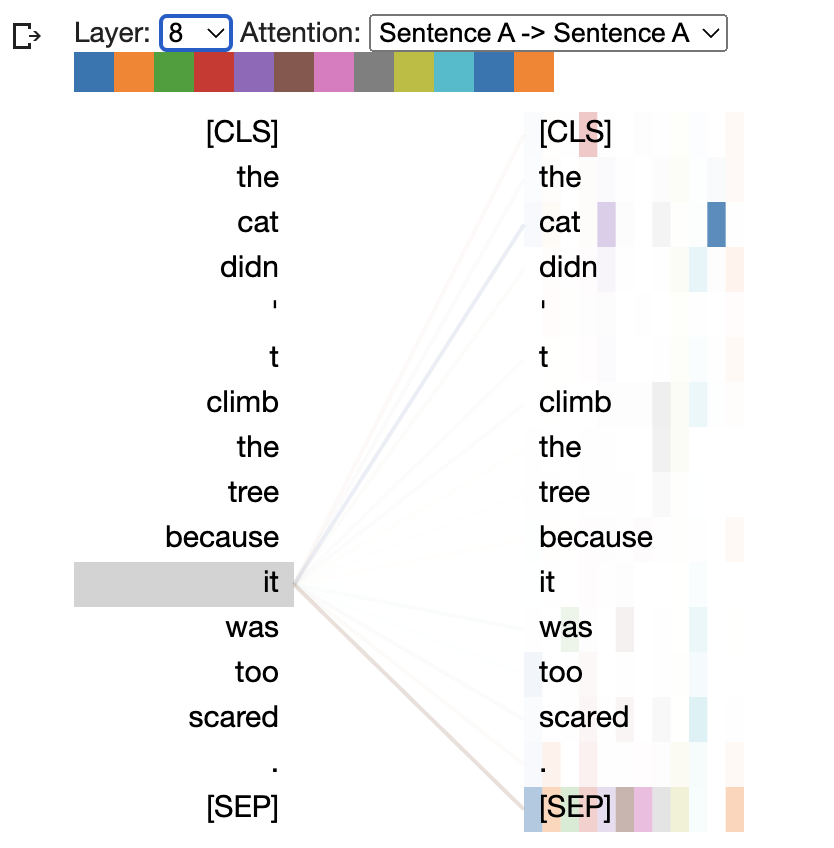
\includegraphics[width=8cm]{pages/imgs/att_self_sample.png}
    \caption{Self-Attention of the sample}
    \label{fig:att_self_sample}
\end{figure}

Capturing the connections between an input and an output sequence is vital for downstream tasks, like Neural Machine Translation (NMT). In this case, the Encoder-Decoder attention mechanism operates in a manner similar to Self-Attention. Let's translate our sample sentence into Portuguese and explore the significant connections it reveals. To accomplish this, we will utilize a pre-trained language model called Multilingual BERT (mBERT), which has knowledge about multiple languages, including English and Portuguese \cite{devlin2018bert}.


\begin{figure}[h]
    \centering
    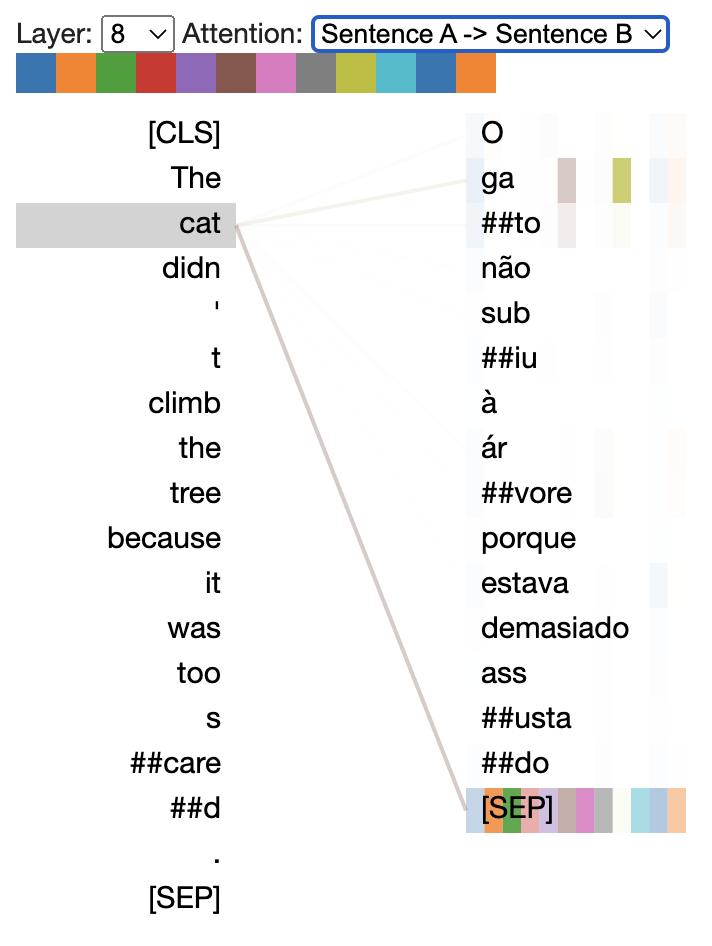
\includegraphics[width=8cm]{pages/imgs/att_cat_sample.png}
    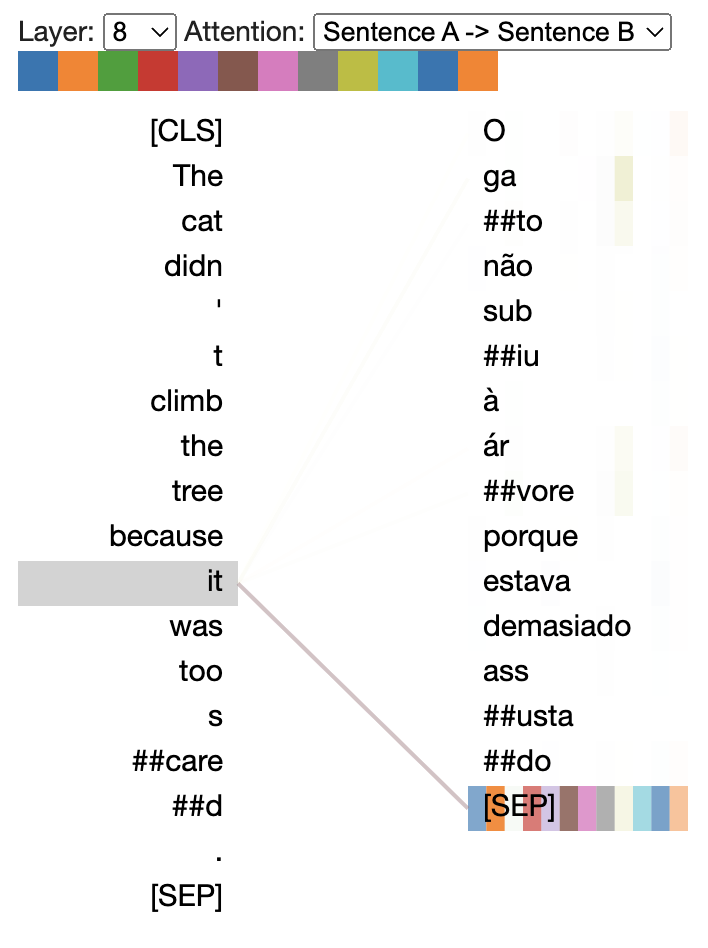
\includegraphics[width=8cm]{pages/imgs/att_it_sample.png}
    \caption{Encoder-Decoder Attention of the sample}
    \label{fig:ed_att_sample}
\end{figure}

In the left image of Figure \ref{fig:ed_att_sample}, we can clearly see that the attention of the token 'cat' is specifically directed towards the token 'gato,' which corresponds to its accurate translation. Similarly, in the right image, the word 'it' is attentively aligned with the token 'gato' once again. These observations indicate the system's ability to effectively focus on the appropriate tokens, both in correctly selecting the appropriate translation, and accurately identifying the relevant noun.

Now let's explore each building block of the Transformer architecture and examine how the Attention mechanism fits in this.



\section{Encoder Architecture}\label{sec:enc}

In the original paper for transformers \citep{vaswani2017attention}, a ``sub-layer`` is formed by either a Feed-Forward ($\mathrm{FF}$) or Multi-Head Attention $\mathrm{MHA}$ (or other named $\mathrm{sub-block}$s) followed by a sequence of operations. In this section, we begin by explaining the encoder architecture. Note that the notation of ``sub-layer`` also applies to the following sections.

\subsection{Simplified Encoder Architecture}

the encoder architecture can be succinctly described as stacking a number of $N$ blocks on top of each other combining a $\mathrm{FF}$ and $\mathrm{MHA}$ sub-blocks. A single block is defined as

\begin{equation}
e^{n+1} = \mathrm{FF}(\mathrm(MHA(e^n)).
\end{equation}

The input to the first block $e^0$ is the sum of position $P$ and non-contextual embeddings $E$ of the input. Assuming $x_1 \cdots x_T$ is a sequence of integers (indices to a vocabulary of $V$ symbols) we have that

\begin{equation}
e^{0}_t = \mathrm{E} \cdot \mathrm{1}_{x_t} + \mathrm{P} \cdot \mathrm{1}_t \quad \mbox{for} \quad t=1 \cdots T
\end{equation}

where $\mathrm{1}_{x_t}$ and $\mathrm{1}_t$ are indicators, i.e. one-hot, vectors for the token content (vocabulary symbol) and the token position. $\mathrm{E} \in \mathbb{R}^{H \times V}$ is the non-contextual embedding matrix for each symbol in the vocabulary and $P^{H \times \tau}$ is the position embedding matrix, where  $\tau-1$ is the furthest position supported. See Figure \ref{fig:e0} for the construction of the input of the first block. \\


\begin{figure}[h]
    \centering
    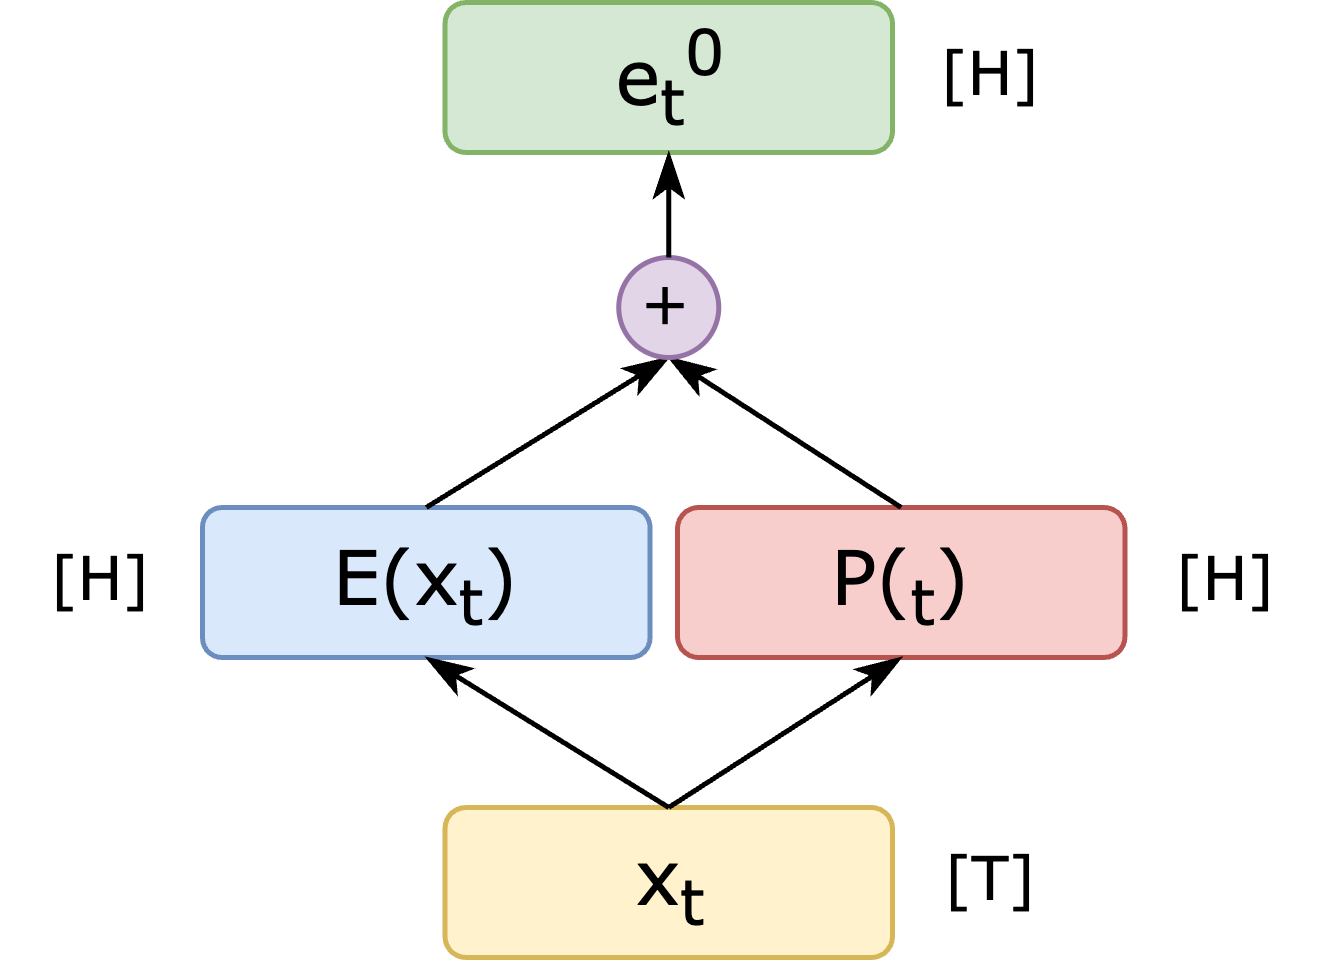
\includegraphics[width=5cm]{pages/imgs/e0.png}
    \caption{Construction of the input of the $t$-th token in layer $e^0$}
    \label{fig:e0}
\end{figure}



\noindent The feed-forward ($\mathrm{FF}$) is given by:

\begin{equation}
FF(z) = W^2\cdot \mathrm{gelu}(W^1 \cdot z)
\end{equation}

\noindent with weight matrices $W^2 \in \mathbb{R}^{H \times 4H}$ and $W^1 \in \mathbb{R}^{4H \times H}$, that expand and contract the hidden dimension $H$.

The Self-Attention ($\mathrm{SA}$) comprises three matrices extracted from the encoder’s input $z$. So, for every given input $z$, we generate a Key vector($K$), a Query vector($Q$), and a Value vector($V$). These matrices are obtained by performing matrix multiplication between the embedding and the corresponding matrix that was learned in the training process, e.g. $Q = W^Q z$.

The next step is to calculate the self-attention score. The Key and Query matrices are multiplied by each other and normalized by a constant value $\frac{1}{A} \left(W^K z\right)^T W^Q z$ or $\frac{1}{A} K^T Q$. The $A$ is usually chosen to be the square root of the dimension of the key matrices. This leads to having more stable gradients.

\noindent Then pass the result through a $softmax$ operation. The Softmax normalizes the scores so they’re all positive and add up to 1. In other words, extracts a distribution of relative scores from a given token for each token in the input sequence.

\noindent After this multiply the output by the Value matrix: $W^V \cdot z \cdot \underset{i \rightarrow}{\mathrm{softmax}}\left( \frac{1}{A} \left(W^K z\right)^T W^Q z \right)$ or simply $V \cdot \underset{i \rightarrow}{\mathrm{softmax}}\left( \frac{1}{A} \left(K \right)^T Q \right)$.

The Multi-Head Attention ($\mathrm{MHA}$) enhances the Self-Attention layer in two ways: it allows the model to focus on different positions within the input, enabling a better understanding of pronoun references; and allowing projection of input embeddings into distinct representation subspaces, thereby improving overall performance.

\noindent Finally getting the following mathematical form for the $\mathrm{MHA}$:


\begin{equation}
MHA(z) =  W^o \cdot
\begin{bmatrix}
    W^V_1 \cdot z \cdot \underset{i \rightarrow}{\mathrm{softmax}}\left( \frac{1}{A} \left(W^K_1 z\right)^T W^Q_1 z \right)\\
    W^V_2 \cdot z \cdot \underset{i \rightarrow}{\mathrm{softmax}}\left( \frac{1}{A} \left(W^K_2 z\right)^T W^Q_2 z \right)\\
    \cdots\\
    W^V_D \cdot z \cdot \underset{i \rightarrow}{\mathrm{softmax}}\left( \frac{1}{A} \left(W^K_D z\right)^T W^Q_D z \right)\\
\end{bmatrix}\nonumber
\end{equation}

where we have $D$ attention heads. Each head contracts the hidden dimension $W^K, W^Q, W^V \in \mathbb{R}^{H / D \times H}$ into a space of size $H / D$ (this has practical implementation consequences). Outputs of all heads are concatenated and projected again with $W^o \in \mathbb{R}^{H \times H}$.

\begin{figure}[h]
    \centering
    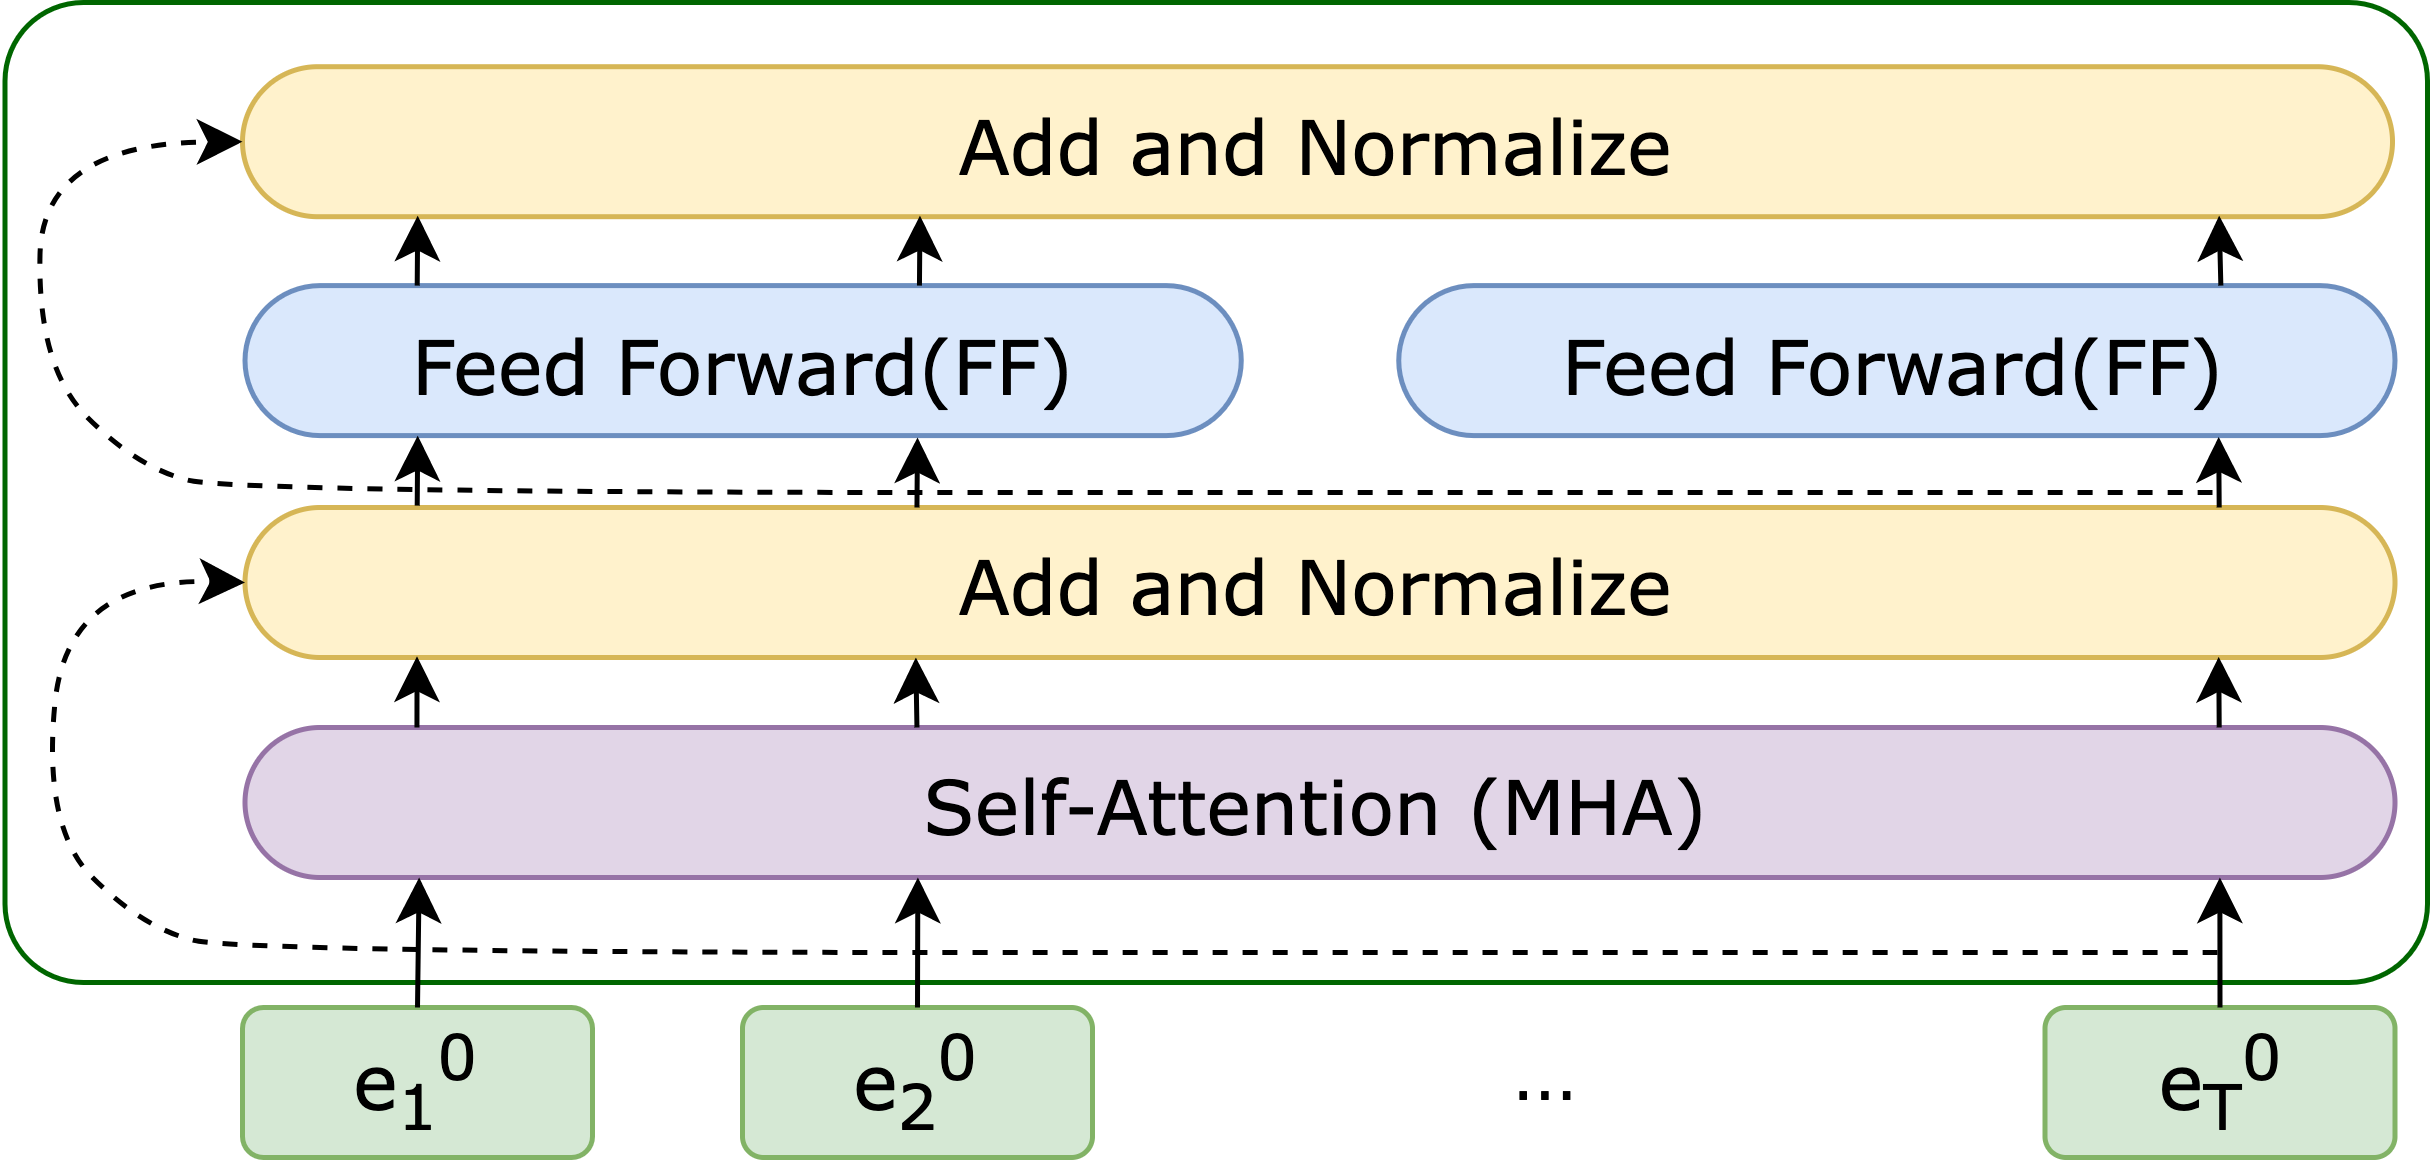
\includegraphics[width=10cm]{pages/imgs/encoder_block.png}
    \caption{Encoder block}
    \label{fig:encoder_block}
\end{figure}




\subsection{Adding Dropout, Residuals, and Layer Normalization}

%For simplicity, we have left several additional operations that can be added as a wrapper around $\mathrm{FF}$ and $\mathrm{MHA}$ operations. These can be expressed as

%\begin{equation}
%C(f)(x) = x + \mathrm{dropout}(f(\mathrm{layernorm}(x)))
%\end{equation}

%where $f = \{\mathrm{FF}, \mathrm{MHA}\}$.

To complete the ``sub-layer``, a dropout followed by a residual connection and a layer normalization is applied to input $z$ that has been passed through a $\mathrm{sub-block}$, where a $\mathrm{sub-block} \in \{\mathrm{FF}, MHA\}$. Together, we can express the function as

\begin{equation}
C(x) = \mathrm{layernorm}(\mathrm{residual}(\mathrm{dropout}(\mathrm{sublayer}(z)), z)
\end{equation}

where $\mathrm{sublayer} \in \{\mathrm{FF}, \mathrm{MHA}\}$.


Specifically, we have
\begin{itemize}
    \item $\mathrm{dropout}(x) = r * x$ where $ r_j \sim \operatorname{Bernoulli}(p)$ and $*$ refers to element-wise multiplication\footnote{Note that the default $p$ is $0.1$.},
    \item $\mathrm{residual}(x, z) = x + z$, and 
    \item $\mathrm{layernorm}(x) = \frac{x-E(x)}{\sqrt{Var(x)+\epsilon}}*\gamma + \beta$ where $E(x)$ and $Var(x)$ are computed among dimensions other than the dimension for the batch\footnote{Note that the default $\epsilon$ is $1e-5$. $\gamma$ and $\beta$ are learnable affine parameters if we want to learn, otherwise set to $1$ and $0$}.
\end{itemize}

After incorporating all of these subcomponents, we obtain the final Encoder block, as illustrated in Figure \ref{fig:encoder_block}

\section{Decoder Architecture}\label{sec:dec}

This is identical to the Encoder architecture with two differences

\begin{enumerate}
    \item We feed if a partial sequence $x_{<t}$ and take the last output $h_{t-1}$ as the hidden vector for $x_t$
    \item We mask every head of $\mathrm{MHA}$ to prevent any value of time $p$ to depend on values of $>p$
\end{enumerate}

The implementation of training realizes 1) by masking input partial sequence $x_{<t}$ and hidden units from the corresponding positions with an attention mask. This attention mask is also applied during inference time. 

\begin{figure}[h]
    \centering
    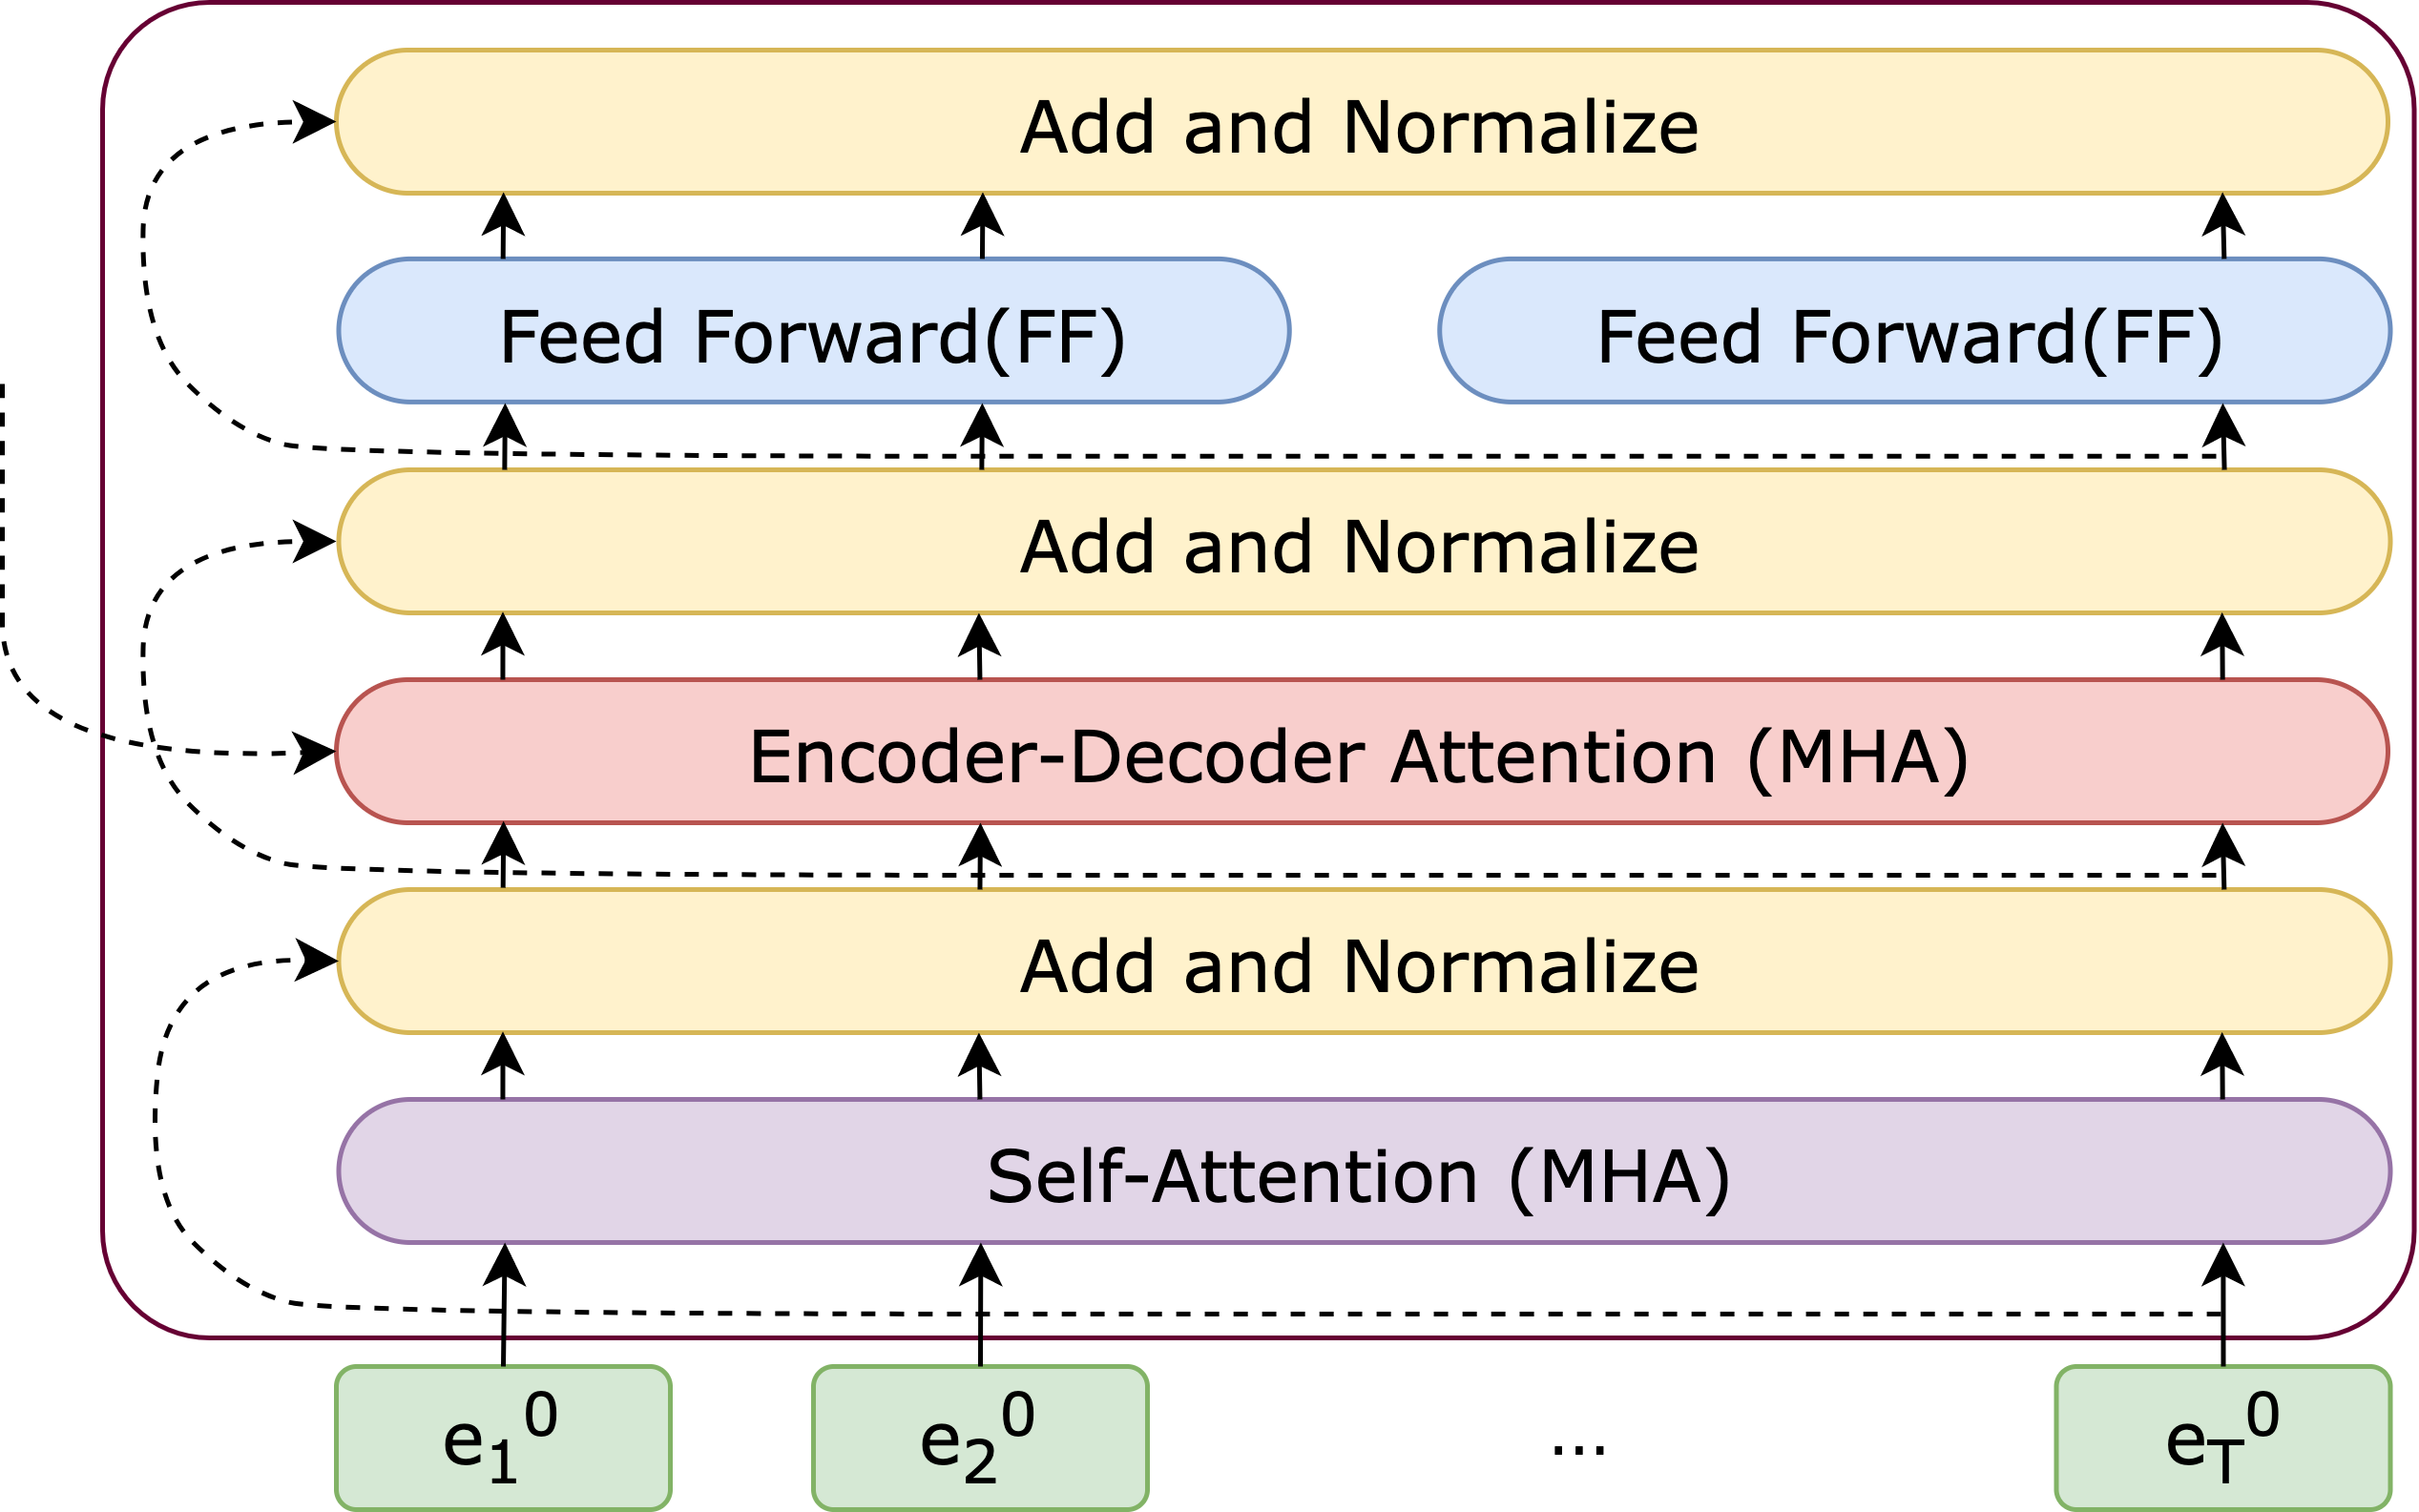
\includegraphics[width=10cm]{pages/imgs/decoder_block.png}
    \caption{Decoder block}
    \label{fig:decoder_block}
\end{figure}

Once all these subcomponents are integrated, we achieve the final Decoder block, which is depicted in Figure \ref{fig:decoder_block}.


\section{Encoder-Decoder Architecture}

In the Encoder-Decoder Architecture, the encoder is the same as section \ref{sec:enc}. Therefore, we have the encoded embeddings as $e^N = \mathrm{Encoder}(x)$.

The decoder in the Encoder-Decoder Architecture is a little bit different than section \ref{sec:dec}. Each layer of the decoder will include one more Cross-Multi-Head Attention (CMHA) sub-layer, and the order of sub-layers in a decoder layer will be $\mathrm{MHA}$-$\mathrm{CMHA}$-$\mathrm{FF}$, i.e.

\begin{equation}
    d^{m+1} = \mathrm{FF}(\mathrm(CMHA(e^N, MHA(d^m))).
\end{equation}

Specifically, the query matrix is computed from the layer below it, while the key and value matrix are computed from $e^N$, which can be expressed as

\begin{equation}
    \mathrm{CMHA}(e^N, MHA(d^m)) = W^o \cdot
\begin{bmatrix}
    W^V_1 \cdot e^N \cdot \underset{i \rightarrow}{\mathrm{softmax}}\left( \frac{1}{A} \left(W^K_1 e^N\right)^T W^Q_1 MHA(d^m) \right)\\
    W^V_2 \cdot e^N \cdot \underset{i \rightarrow}{\mathrm{softmax}}\left( \frac{1}{A} \left(W^K_2 e^N\right)^T W^Q_2 MHA(d^m) \right)\\
    \cdots\\
    W^V_D \cdot e^N \cdot \underset{i \rightarrow}{\mathrm{softmax}}\left( \frac{1}{A} \left(W^K_D e^N\right)^T W^Q_D MHA(d^m) \right)\\
\end{bmatrix}\nonumber.
\end{equation}


\begin{figure}[h]
    \centering
    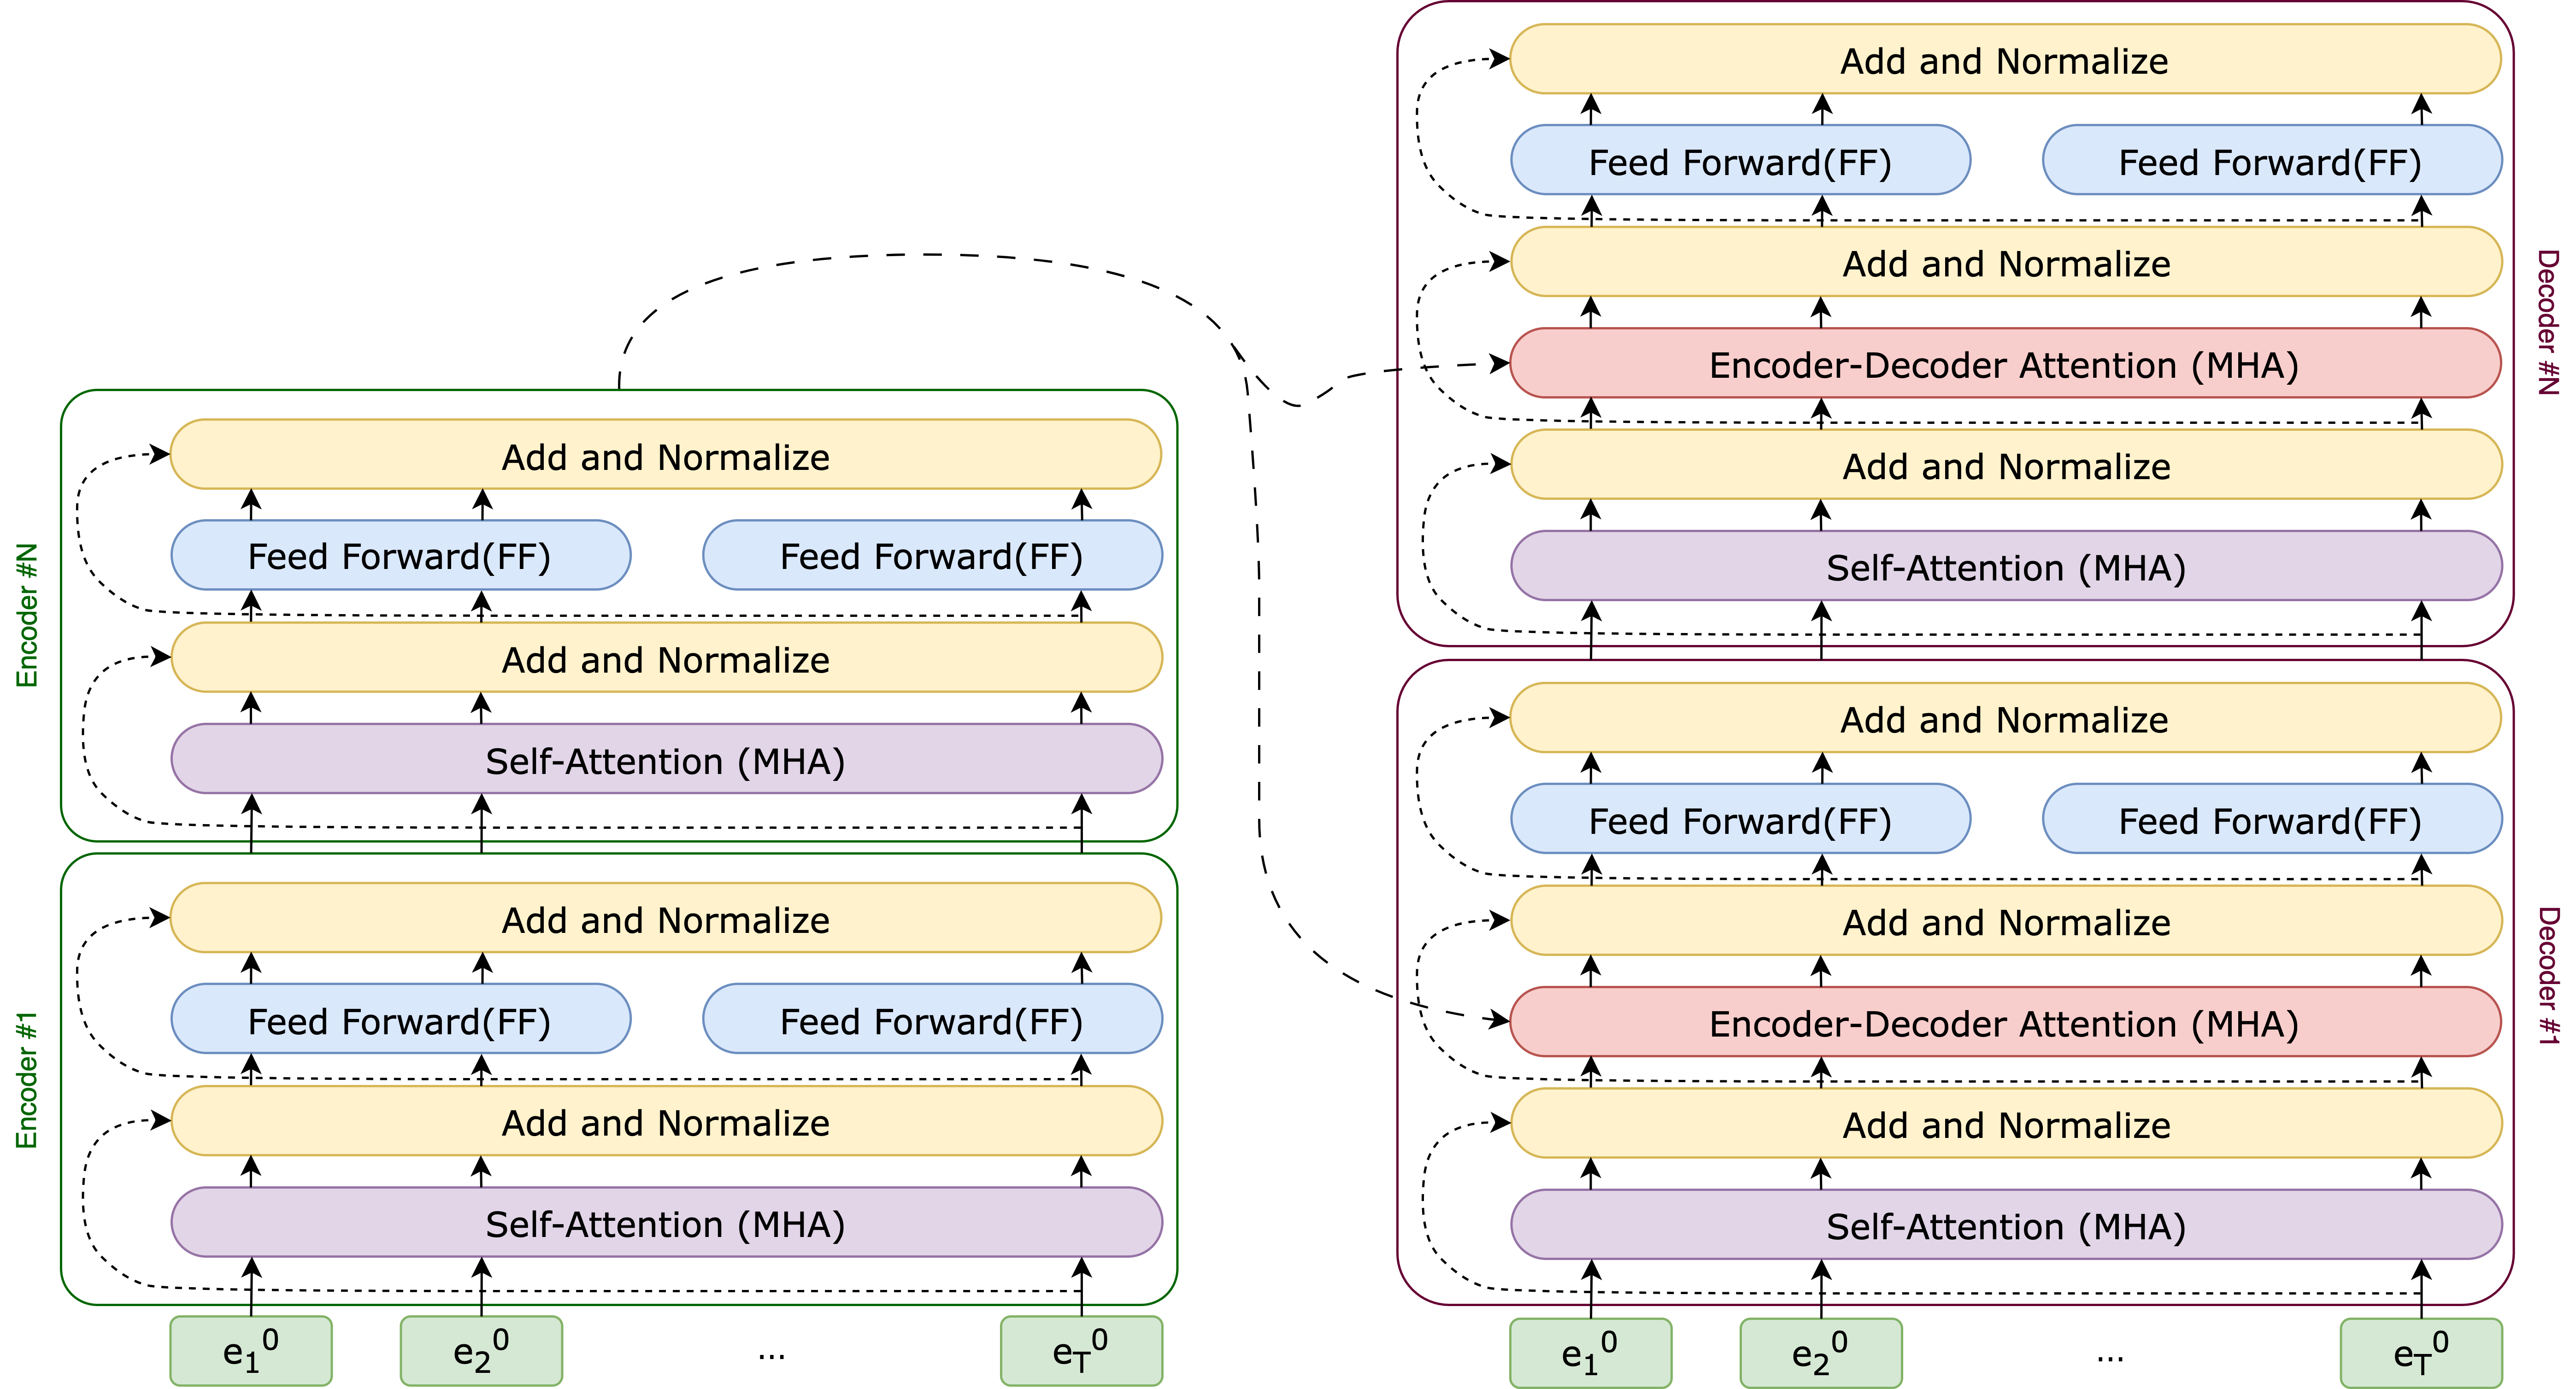
\includegraphics[width=16cm]{pages/imgs/encoder_decoder.png}
    \caption{Encoder-Decoder Architecture}
    \label{fig:encoder_decoder}
\end{figure}


By combining $N$ blocks of Encoder and Decoder, we obtain the complete view of the Transformer architecture, as illustrated in Figure \ref{fig:encoder_decoder}.



\begin{exercise} 
Cross Multi-Head Attention \& Multi-Head Attention
Now let's implement our own Attention mechanism, to that end let's:
\begin{enumerate}
\item Complete the {\tt cross\_attention} function. Given two input sequences $S_1$ and $S_2$ and the transformation weights $W_Q$, $W_K$, and $W_V$. You need to implement the following:
\begin{enumerate}
    \item Calculate the query, key, and value projections using linear transformations.
    \item Compute the attention scores by performing the dot product between the query and key tensors.
    \item Apply softmax activation to the attention scores to obtain the attention weights.
    \item Multiply the attention weights with the value tensor to get the attended values.
    \item Return the attended values.
\end{enumerate}


\begin{python}
import torch
import torch.nn.functional as F

def cross_attention(S1, S2, W_Q, W_K, W_V):
    ## Your code here
    return attended_values
\end{python}
\item Complete the {\tt CausalSelfAttention} class. First, you should create linear projections {\tt query\_proj}, {\tt key\_proj} and {\tt value\_proj}.
\begin{python}
import math
import torch.nn as nn

class CausalSelfAttention(nn.Module):

    def __init__(self, config):
        super().__init__()
        
        # Initialize layers and parameters
        self.hidden_size = config.n_embd
        self.num_heads = config.n_head

        # TODO: Create the linear projections

        self.output_proj = nn.Linear(config.n_embd, config.n_embd)

        self.attn_dropout = nn.Dropout(config.attn_pdrop)
        self.resid_dropout = nn.Dropout(config.resid_pdrop)

        self.register_buffer(
            "bias",
            torch.tril(torch.ones(config.block_size, config.block_size)).view(
                1, 1, config.block_size, config.block_size))
\end{python}
Then apply {\tt query\_proj}, {\tt key\_proj} and {\tt value\_proj} to split input into query, key, and value tensors:
\begin{python}
    def forward(self, x: torch.Tensor) -> torch.Tensor:
        B, T, C = x.size()

        # TODO: Split input into query, key, and value tensors

        # Reshape and transpose tensors for multi-head computation
        query = query.view(B, T, self.num_heads,
                           self.hidden_size // self.num_heads).transpose(1, 2)
        key = key.view(B, T, self.num_heads,
                       self.hidden_size // self.num_heads).transpose(1, 2)
        value = value.view(B, T, self.num_heads,
                           self.hidden_size // self.num_heads).transpose(1, 2)
\end{python}
Then compute the attention scores. Note that the shape of scores should be {\tt (B, num\_heads, T, T)}
\begin{python}
        # TODO: Compute attention scores

        # Apply a causal mask to restrict attention to the left in the input sequence
        mask = self.bias[:, :, :T, :T]
        scores = scores.masked_fill(mask == 0, float('-inf'))
\end{python}
Finally, apply soft-max activation and multiply attention weights with values to get attended values:
\begin{python}
        # TODO: Apply softmax activation to get attention weights

        # TODO: Multiply attention weights with values to get attended values

        # Transpose and reshape attended values to restore original shape
        attended_values = attended_values.transpose(1, 2).contiguous().view(
            B, T, C)

        # Apply output projection and dropout
        output = self.resid_dropout(self.output_proj(attended_values))

        return output
\end{python}
\end{enumerate}
\end{exercise}

\section{Training different Transformers}
We have introduced different architectures of transformers and will present different variants of transformers that are trained with different objectives, and thus applied to different downstream tasks. We briefly introduce all these transformers and provide references so you can read these papers if you are interested.

\subsection{Training with Encoders}
Encoder models solely utilize the encoder component of a Transformer model. In each step, the attention layers have the ability to consider all the words present in the original sentence. These models are known as 'auto-encoding models' and are recognized for their 'bi-directional' attention mechanism.

The pretraining of these models typically involves manipulating a given sentence, often by obscuring random words and assigning the model the task of identifying or reconstructing the original sentence. This objective is commonly referred to as Masked Language Modeling (MLM), and models pre-trained with this objective are known as Masked Language Models.

For a text sequence $\textbf{x}$, the BERT model first constructs a corrupted version $\hat{\textbf{x}}$. Let the masked tokens be $\bar{\textbf{x}}$. The training objective is to reconstruct $\bar{\textbf{x}}$ from $\hat{\textbf{x}}$:

\begin{align}
max_{\theta}logP_{\theta}(\bar{\textbf{x}}|\hat{\textbf{x}})\approx \sum_{t=1}^Tm_tlogP_{\theta}(x_t|\hat{\textbf{x}})
=\sum_{t=1}^Tm_tlog\frac{exp(H_{\theta}(\hat{\textbf{x}})_t^Te(x_t))}{\sum_{x\prime} {exp(H_{\theta}(\hat{\textbf{x}})_t^Te(x\prime)}}
\end{align}

Where the $\approx$ indicates that all $\bar{\textbf{x}}$ elements are independent (seperately reconstructed), $m_t$ indicates weather or not $x_t$ is masked (1-masked, 0-not), $H_{\theta}$ is a Transformer that maps a sequence $x$ of length $T$ and contains infomation about the context on both sides $H_{\theta}(X)=[H_{\theta}(x)_1, H_{\theta}(x)_2,...H_{\theta}(x)_T]$, and $e(x)$ denotes the embedding of $x$.

Encoder models excel in tasks that demand a comprehensive understanding of the entire sentence. These tasks include sentence classification, word classification tasks e.g. named entity recognition, and extractive question answering. Widely used representatives of this model family include BERT \cite{devlin2018bert} and RoBERTa \cite{liu2019roberta}.

\textbf{BERT} \cite{devlin2018bert} is trained on MLM(Masked Language Modeling) and NSP(Next Sentence Prediction) objectives.
In the \textbf{MLM} objective, 15\% of the input tokens are selected. Among these selected tokens:
\begin{itemize}
    \item 80\% of the time, the mask token is inserted in place of the original token.
    \item 10\% of the time, a random token is inserted in place of the original token.
    \item 10\% of the time, the original token remains unchanged.
\end{itemize}
The \textbf{NSP} objective is applied to pairs of sentences, A and B, taken from the training set. In 50\% of the cases, sentence B directly follows sentence A in the input, while in other cases, the pairs are randomly selected. The objective is to perform binary classification and predict whether sentence B follows sentence A or not.

\textbf{RoBERTa} \cite{liu2019roberta} builds upon BERT's pre-training by addressing its perceived undertraining. It introduces the following modifications:
\begin{itemize}
    \item Longer and larger-scale training: RoBERTa trains the model for an extended period using larger batches, more data, and longer sequences.
    \item Removal of NSP objective: The next sentence prediction (NSP) objective, present in BERT, is eliminated in RoBERTa.
    \item Dynamic masking: RoBERTa employs dynamic masking by duplicating the training data ten times and applying different mask patterns to each sample. This contrasts with BERT's static masking, where a fixed mask is used for each sample.
\end{itemize}
These modifications aim to enhance RoBERTa's pre-training performance and overall language understanding capabilities.




\subsection{Training with Decoders}
Decoder-only or Autoregressive modeling performs
pretraining by maximizing the likelihood under the forward autoregressive factorization:
$$
max_{\theta}logP_{\theta}(\textbf{x})=\sum_{t=1}^TlogP_{\theta}(x_t|\textbf{x}_{<t})
= \sum_{t=1}^T{log\frac{exp(h_{\theta}(\textbf{x}_{1:t-1})^Te(x_t))}{\sum_{x\prime}exp(h_{\theta}(\textbf{x}_{1:t-1})^Te(x\prime))}}
$$

Where the $h_{\theta}(\textbf{x}_{1:t-1})$ is the context representation produced by the neural model, and it contains information (conditioned) about the tokens up to position $t$, and $e(x_t)$ is the embedding of a token $x_t$.

A Decoder-only or Autoregressive model operates differently compared to Encoder-only or Autoencoder model by focusing on density estimation rather than reconstructing corrupted input. These models aim to estimate probability distributions, which limits their ability to capture bidirectional context. As a result, they are restricted to uni-directional processing.

\paragraph{GPTs.} The class of GPTs is a series of pre-trained decoder-only transformers. Models are pre-trained to perform the next token prediction with the Cross-Entropy criterion. Since the release of GPT-1 \citep{gpt-1}, GPTs are being trained with more parameters and training data, with GPT-2 \citep{gpt-2}, GPT-3 
\citep{gpt-3}, InstructGPT \citep{instructgpt} and GPT-4 \citep{gpt-4} being subsequently released. Note that since the release of InstructGPT \citep{instructgpt}, this class of language models has been trained with reinforcement learning with human feedback \citep{rlhf}, which enables the model to manifest interesting behaviors that you see when using ChatGPT.


\subsection{Training with Encoder-Decoder}
To leverage the strengths of both Encoder-only and Decoder-only models, the concept of Encoder-Decoder models was introduced. While previous methods effectively captured bidirectional information for text generation, they had certain limitations in terms of contextual token representations. One common approach involved concatenating the left-to-right and right-to-left representations \cite{peters2018deep}.

Encoder-Decoder models aim to overcome these limitations by combining the advantages of both approaches. These models can effectively capture bidirectional information while maintaining robust contextual representations for each token. By leveraging the strengths of both encoders and decoders, Encoder-Decoder models offer enhanced capabilities for various natural language processing tasks, including text generation.

Commonly employed members of this model family include BART \cite{lewis-etal-2020-bart} and T5 \cite{raffel2020exploring}, which have gained significant popularity in the field.

\paragraph{BART.} BART \cite{lewis-etal-2020-bart} an encoder-decoder model pre-trained on five tasks injecting noises into the input text: i) token masking (same as BERT \cite{devlin2018bert}), ii) token deletion, iii) text infilling by replacing sampled input spans with single masks, iv) sentence permutation, and v) document rotation. The powerful pre-trained denoising autoencoder is commonly used in generation tasks.

\paragraph{T5.} T5 (Raffel et al., 2020) utilizes a text-to-text methodology. In this approach, various tasks like translation, question answering, and classification are transformed into a unified format. The model is provided with input text and trained to generate the corresponding output text. To achieve this, a task-specific prefix(instruction) is added to the input sequence, and the model is pre-trained to produce outputs specific to each task.\\



\begin{exercise} Training Transformers

Let's delve into practical training of a Transformer model to gain hands-on experience. Our initial step will involve creating a Decoder-based model (GPT-2 \cite{gpt-2}) and training it on a modest dataset. Once this is completed, we can visualize the attention mechanism before and after the training process. Finally, we can compare the performance of the trained model during inference with that of the smaller trained model.


\begin{exercise} Training a Weather Prediction Model Using Autoregressive Transformer.

In this exercise, we will be working with a dummy weather dataset comprising sequences of weather observations and their corresponding states. The objective is to train a compact autoregressive transformer model that can predict the weather state based on previous observations.
Let's begin by importing the required modules and classes, and setting a seed value to ensure consistent output every time we run the file.

\begin{python}
import random
import time

import numpy as np
import torch
from torch.utils.data.dataloader import DataLoader

random.seed(42)

from lxmls.transformers.bpe import BPETokenizer
from lxmls.transformers.dataset import WeatherDataset
from lxmls.transformers.model import GPT
from lxmls.transformers.trainer import Trainer
from lxmls.transformers.utils import set_seed
\end{python}

\end{exercise}

To begin, we initialize the training dataset, which comprises sequences of weather observations along with their corresponding states. These sequences are transformed into indices and then concatenated to create the input and output sequences for the transformer model. For more information on this, refer to: "lxmls/transformers/dataset.py".

\begin{python}
fixed_proba = {}
fixed_proba["initial"] = [0.5, 0.3, 0.2]
fixed_proba["transition"] = [[0.5, 0.5, 0], [0, 0.5, 0.5], [0.5, 0, 0.5]]
fixed_proba["emission"] = [
    [0.5, 0, 0.2, 0, 0.3],
    [0, 0.5, 0.4, 0, 0.1],
    [0, 0, 0.1, 0.5, 0.4],
]

\end{python}

Let's print an example instance of the dataset.
\begin{python}
train_dataset = WeatherDataset("train", proba=fixed_proba)
test_dataset = WeatherDataset("test", proba=train_dataset.proba)
x, y = train_dataset[0]

print("Sampling from the dataset:")
print(f"Input: {train_dataset.decode_obs(x.tolist()[:6])}")
print(f"Labels: {train_dataset.decode_st(y.tolist()[5:])}")
print("-" * 50)
print("Tokenized sequences:")
print(f"Input: {x.tolist()}")
print(f"Labels: {y.tolist()}")
\end{python}

Moving forward, we construct a model using the default configuration for the GPT model, which encompasses parameters defining the model's size and structure. In this case, we employ a compact variant known as GPT Nano.

\begin{python}
model_config = GPT.get_default_config()
model_config.model_type = "gpt-nano"
model_config.vocab_size = train_dataset.get_vocab_size()
model_config.block_size = train_dataset.get_block_size()
model = GPT(model_config)

print(model_config)
\end{python}

To facilitate the training of our model, we instantiate a Trainer object. The Trainer manages various aspects of the training process, such as configuring the learning rate, specifying the maximum number of iterations, and determining the number of workers for data loading. We initialize the Trainer with the model, training dataset, and validation dataset.

\begin{python}
train_config = Trainer.get_default_config()
train_config.learning_rate = (
    5e-4  # The model we're using is so small that we can go a bit faster
)
train_config.max_iters = 2000
train_config.num_workers = 0
train_config.device = "mps"
trainer = Trainer(train_config, model, train_dataset)

print(train_config)
\end{python}

With all these components in position, we are fully prepared to train our model using the weather dataset and leverage the acquired patterns to generate predictions.

\begin{python}
def batch_end_callback(trainer):
    if trainer.iter_num % 100 == 0:
        print(
            f"iter_dt {trainer.iter_dt * 1000:.2f}ms; iter {trainer.iter_num}: train loss {trainer.loss.item():.5f}"
        )


trainer.set_callback("on_batch_end", batch_end_callback)

start_time = time.time()
trainer.run()
end_time = time.time()
elapsed_time = end_time - start_time

# Print the training time
print("Training time: {:.2f} seconds".format(elapsed_time))
\end{python}

Now, let's visualize the attention heads of our trained model. To do this, we need to install the HF transformers and bertviz packages. You can install them by running the following command: "pip install transformers bertviz".


\begin{python}
from transformers import BertTokenizer, BertModel
from bertviz import head_view

# Define a sample input text
text = "I will go for a run and will jump into a lake."

# Instantiate the BERT tokenizer and model
tokenizer = BertTokenizer.from_pretrained("bert-base-uncased")
model = BertModel.from_pretrained("bert-base-uncased")

# Tokenize the input text
tokens = tokenizer.tokenize(text)

# Convert tokens to token IDs
token_ids = tokenizer.convert_tokens_to_ids(tokens)

# Create attention mask
attention_mask = [1] * len(token_ids)

# Convert token IDs and attention mask to tensors
input_ids = torch.tensor([token_ids])
attention_mask = torch.tensor([attention_mask])

# Generate the transformer output
outputs = model(input_ids, attention_mask=attention_mask, output_attentions=True)

head_view(outputs.attentions, tokens=tokens)
\end{python}



\begin{exercise} Promoting a GPT-2 model
Now that we have trained our own Transformer model and gained some understanding of its functioning, let's explore a larger pre-trained model that has been trained on a vast amount of natural data. By doing so, we can experience generating output that closely resembles human-like responses.

\begin{python}
model_type = "gpt2"
device = "mps"

model = GPT.from_pretrained(model_type)

# move model to the device(GPU if available)
# set to eval mode to avoid gradient accumulation
model.to(device)
model.eval()

# Random prompt, uses pooling
for i in range(5):
    set_seed(42)
    model.prompt("Barack Obama, the", 50, 3)

# Deterministic prompt, does NOT use pooling
for i in range(5):
    model.prompt_topK("Barack Obama, the", 50, 3)
\end{python}

Get ready to embark on an intriguing journey by playing with the input prompt and witnessing the fascinating and captivating outputs that await you!

\end{exercise}

\end{exercise}


%\chapter{\label{day:seq_disc}Learning Structured Predictors}
%In this class, we will continue to focus on sequence classification,
but instead of following a \emph{generative} approach (like in the previous
chapter) we move towards \emph{discriminative} approaches. Recall that the difference between these approaches is that generative approaches attempt to model the probability distribution of the data, $P(X,Y)$, whereas discriminative ones only model the conditional probability of the sequence, given the observed data, $P(Y|X)$.



\section*{Today's Assignment}

The assignment of today's class is to implement the structured version of the perceptron algorithm.

\section{Classification vs Sequential Classification}


Table \ref{disc_seq_summary} shows how the models for classification 
have counterparts in \emph{sequential} classification. In fact, in
the last chapter we discussed the Hidden Markov model, which can be seen as a
generalization of the Na\"{i}ve Bayes model for sequences. 
In this chapter, we will see a generalization of the
Perceptron algorithm for sequence problems (yielding the Structured
Perceptron, \citealt{collins2002discriminative}) and a generalization of
Maximum Entropy model for sequences (yielding Conditional Random Fields, \citealt{lafferty2001conditional}). 
Note that both these generalizations are  not specific for sequences
and can be applied to a wide range of models (we will see in tomorrow's
lecture how these methods can be applied to parsing).
Although we will not cover all the methods described in
Chapter \ref{day:classification}, bear in mind that all of those have a structured counterpart. 
It should be intuitive after this lecture how those methods could be
extended to structured problems, given the perceptron example.
%Before we explain the particular methods, the next section will talk a bit about feature representation for sequences. 

\begin{table}[ht]
\centering
\begin{tabular}{|l|l|}
\hline
\multicolumn{1}{|c|}{\textbf{Classification}} & \multicolumn{1}{|c|}{\textbf{Sequences}} \\
\hline
\multicolumn{2}{|c|}{\emph{Generative}}\\
\hline
Na\"{i}ve Bayes~(Sec.~\ref{s::naiveBayes}) & Hidden Markov Models~(Sec.~\ref{hmm}) \\
\hline
\multicolumn{2}{|c|}{\emph{Discriminative}}\\
\hline
Perceptron~(Sec.~\ref{s:perceptron}) & Structured Perceptron~(Sec.~\ref{s:spercetron})\\
\hline
Maximum Entropy~(Sec.~\ref{s:me}) & Conditional Random Fields~(Sec.~\ref{s:crf})\\
\hline
\end{tabular}
\caption{\label{disc_seq_summary}Summary of the methods used for classification and sequential classification covered in this guide.}
\end{table}


Throughout this chapter, we will be searching for the solution of 
\begin{equation}
\argmax_{y \in \statevocab^N} P(Y=y | X=x) = \argmax_{y \in \statevocab^N} \W \cdot  \F(x,y). \label{eq::struc_pred} 
\end{equation}
where $\W$ is a weight vector, and $\F(x,y)$ is a feature vector. We will see that this sort of linear models are more flexible than HMMs, in the sense that they may incorporate 
more general features while being able to reuse the same decoders (based on the Viterbi and forward-backward algorithms). In fact, \emph{the exercises in this lab will not touch the decoders that 
have been developed in the previous lab}. \todo{nao percebo muito bem esta nota em italico... Ou � "in fact, .. will touch" ou "However, ... will touch."} Only the training algorithms and the function that 
compute the scores will change.

As in the previous section, $y = y_1\ldots y_N$ is a sequence so the maximization
is over an exponential number of objects, making it intractable by brute force methods. Again
we will make an assumption analogous to the ``first order Markov independence property,'' so that the
features may decompose as a sum over nodes and edges in a trellis. 
This is done by assuming that expression~\ref{eq::struc_pred} can be written as:
\begin{equation}
\argmax_{y \in \statevocab^N} 
\sum_{i=1}^N \underbrace{\W \cdot \F_{\mathrm{emiss}}(i,x,y_i)}_{\mathrm{score}_{\mathrm{emiss}}}  + 
\underbrace{\W \cdot \F_{\mathrm{init}}(x,y_1)}_{\mathrm{score}_{\mathrm{init}}}  + 
\sum_{i=1}^{N-1} \underbrace{\W \cdot \F_{\mathrm{trans}}(i,x,y_i,y_{i+1})}_{\mathrm{score}_{\mathrm{trans}}}+ 
\underbrace{\W \cdot \F_{\mathrm{final}}(x,y_N)}_{\mathrm{score}_{\mathrm{final}}}
\label{eq::struc_pred_decompose}
\end{equation}
In other words, the scores ${\mathrm{score}_{\mathrm{emiss}}}$, 
${\mathrm{score}_{\mathrm{init}}}$, ${\mathrm{score}_{\mathrm{trans}}}$
and ${\mathrm{score}_{\mathrm{final}}}$ are now computed as inner products 
between weight vectors and feature vectors rather than log-probabilities.
The feature vectors depend locally on the output variable 
(\emph{i.e.}, they only look at a single $y_i$ or a pair $y_i,y_{i+1}$);
however they may depend globally on the observed input $x=x_{1},\ldots,x_{N}$.


\section{\label{seq::features} Features}

In this section we will define two simple feature sets.\footnote{Although not required, all the features we will use are binary features, indicating whether a given condition 
is satisfied or not.} The first feature set
will only use identity features, and will mimic the features used by
the HMM model from the previous section. This will allow us to directly
compare the performance of a generative vs a discriminative
approach. %\begin{example}
%Simple ID Feature set containing the same features as an HMM model.
%\begin{python}
%0 Ms./NOUN NF: id:Ms.::NOUN init_tag:NOUN 
%1 Haag/NOUN NF: id:Haag::NOUN EF: prev_tag:NOUN::NOUN 
%2 plays/VERB NF: id:plays::VERB EF: prev_tag:NOUN::VERB 
%3 Elianti/NOUN NF: id:Elianti::NOUN EF: prev_tag:VERB::NOUN 
%4 ./. NF: id:.::. EF: last_prev_tag:NOUN::. 
%\end{python}
%\end{example}
Table~\ref{id-features} depicts the features that are implicit in the HMM, which was the subject of 
the previous chapter. These features are indicators of initial, transition, final, and emission events.

\begin{table}[ht]
\begin{center}
\begin{tabular}{|l|l|}
\hline
Condition & Name\\
\hline
$y_i = c_k \text{  } \& \text{  } i =0 $& Initial Features \\
\hline
$y_i = c_k \text{  } \& \text{  } y_{i-1} = c_l$& Transition Features \\
\hline
$y_i = c_k \text{  } \& \text{  } i = N$& Final Features \\
\hline
$x_i = w_j \text{  } \& \text{  } y_i = c_k$ & Emission Features \\
\hline
\end{tabular}
\caption{\label{id-features} {\tt IDFeatures} feature set. This set
  replicates the features used by the HMM model.}
\end{center}
\end{table}
 
 
Note that the fact that we were using a generative model has forced us (in some sense) to 
make strong independence assumptions. 
However, since we now move to a discriminative approach, where we model $P(Y|X)$ rather than $P(X,Y)$, we are not tied anymore to 
some of these assumptions. In particular: 
\begin{itemize}
\item We may use ``overlapping'' features, \emph{e.g.}, features that fire simultaneously for many instances. 
For example, we can use a feature for a word, such as a feature which fires for the word "brilliantly", and another for prefixes and suffixes of that word, such as one which fires if the last two letters of the word are "ly".
This would lead to an awkward model if we wanted to insist on a generative approach. 
\item We may use features that depend arbitrarily on the \emph{entire input sequence} $x$. On the other hand, 
we still need to resort to ``local'' features with respect to the \emph{outputs} (\emph{e.g.} looking only at consecutive state pairs), 
otherwise decoding algorithms will become more expensive.  
\todo{NOTA-MA: Nos HMM (de order superior) tb, certo?}
\end{itemize}


This leads us to the second feature set, composed of features that are traditionally used in POS tagging with discriminative models. See Table~\ref{ex-features} for some examples.
Of course, we could have much more complex features, looking arbitrarily to 
the input sequence. We are not going to have them in this
exercise only for performance reasons (to have less features and smaller caches). State-of-the-art sequence classifiers can easily reach over one million features!

\begin{table}[h!t]
\begin{center}
\begin{tabular}{|l|l|}
\hline
Condition & Name\\
\hline
$y_i = c_k \text{  } \& \text{  } i =0 $& Initial Features \\
\hline
$y_i = c_k \text{  } \& \text{  } y_{i-1} = c_l$& Transition Features \\
\hline
$y_i = c_k \text{  } \& \text{  } i = N$& Final Features \\
\hline
$x_i = w_j \text{  } \& \text{  } y_i = c_k$& Basic Emission Features \\
$x_i = w_j \text{  } \& \text{ $w_j$ is uppercased} \text{  } \& \text{  } y_i = c_k$& Uppercase Features
\\
$x_i = w_j \text{  } \& \text{ $w_j$ contains digit} \text{  } \& \text{  } y_i = c_k$& Digit Features
\\
$x_i = w_j \text{  } \& \text{ $w_j$ contains hyphen} \text{  } \& \text{  } y_i = c_k$& Hyphen Features
\\
$x_i = w_j \text{  } \& \text{  } w_j[0..i] \forall i \in [1,2,3]
\text{  } \& \text{  } y_i = c_k$& Prefix Features \\
$x_i = w_j \text{  } \& \text{  } w_j[|w_j|-i..|w_j|] \forall i \in [1,2,3] \text{  } \& \text{  } y_i = c_k$& Suffix Features \\
\hline
\end{tabular}
\caption{\label{ex-features} {\tt Extended} feature set. Some features in this set could not be included in the HMM model. The features included in the bottom row are all considered emission features 
for the purpose of our implementation, since they all depend on $i$, $x$ and $y_i$.}
\end{center}
\end{table}



%\begin{example}
%
%\begin{python}
%0 Ms./NOUN NF: id:Ms.::NOUN uppercased::NOUN suffix:.::NOUN suffix:s.::NOUN prefix:M::NOUN prefix:Ms::NOUN init_tag:NOUN 
%1 Haag/NOUN NF: id:Haag::NOUN uppercased::NOUN suffix:g::NOUN suffix:ag::NOUN suffix:aag::NOUN prefix:H::NOUN prefix:Ha::NOUN prefix:Haa::NOUN rare::NOUN EF: prev_tag:NOUN::NOUN 
%2 plays/VERB NF: id:plays::VERB EF: prev_tag:NOUN::VERB 
%3 Elianti/NOUN NF: id:Elianti::NOUN uppercased::NOUN suffix:i::NOUN suffix:ti::NOUN suffix:nti::NOUN prefix:E::NOUN prefix:El::NOUN prefix:Eli::NOUN rare::NOUN EF: prev_tag:VERB::NOUN 
%4 ./. NF: id:.::. EF: last_prev_tag:NOUN::. 
%\end{python}
%\end{example}



Our features subdivide into two groups: 
$\F_{\mathrm{emiss}}$, $\F_{\mathrm{init}}$, 
and $\F_{\mathrm{final}}$ are all instances of 
\emph{node features}, 
depending only on a single position in the
state sequence (a node in the trellis); 
$\F_{\mathrm{trans}}$ 
are \emph{edge features},
depending on two consecutive positions in the state 
sequence (an edge in the trellis).
Similarly as in the previous chapter, we have the following scores (also called 
\emph{log-potentials} in the literature on CRFs and graphical models):
\begin{itemize}
\item \emph{Initial scores.}
These are scores for the initial state. 
They are given by 
\begin{equation}
{\mathrm{score}}_{\mathrm{init}}(x,y_1) = \W \cdot \F_{\mathrm{init}}(x,y_1).
\end{equation} 
\item \emph{Transition scores.}
These are scores for two consecutive states at a particular position. 
They are given by 
\begin{equation}
{\mathrm{score}}_{\mathrm{trans}}(i,x,y_i,y_{i+1}) = \W \cdot \F_{\mathrm{trans}}(i,x,y_{i},y_{i+1}).
\end{equation} 
\item \emph{Final scores.}
These are scores for the final state. 
They are given by 
\begin{equation}
{\mathrm{score}}_{\mathrm{final}}(x,y_N) = \W \cdot \F_{\mathrm{final}}(x,y_N).
\end{equation} 
\item \emph{Emission scores.}
These are scores for a state at a particular position. 
They are given by 
\begin{equation}\label{dis_node_potentials}
{\mathrm{score}}_{\mathrm{emiss}}(i,x,y_i) = \W \cdot \F_{\mathrm{emiss}}(i,x,y_i).
\end{equation} 
\end{itemize}
%which form a vector $\boldsymbol{f}_N(\sent,\hv_i)$, 
%and \emph{edge features}, which form a vector $\boldsymbol{f}_E(\sent,\hv_i,\hv_{i-1})$.% 
%\footnote{To make things simpler, we will assume later on that edge features do not depend on the input $\sent$---but they could, without 
%changing at all the decoding algorithm.} %
%These feature vectors will receive parameter vectors $\boldsymbol{\theta}_N$ and  $\boldsymbol{\theta}_E$. 
%Similarly as in the previous chapter, we consider:
%\begin{itemize}
%\item\emph{Node Potentials.} These are scores for a state at a particular position. 
% They are given by 
% \begin{equation}\label{dis_node_potentials}
% \psi_V(\sent,\hs_i) = \exp(\boldsymbol{\theta}_V \cdot \boldsymbol{f}_V(\sent,\hs_i)).
% \end{equation}
%\item\emph{Edge Potentials.} These are scores for the transitions. They are given by 
% \begin{equation}\label{dis_edge_potentials}
%\psi_E(\sent,\hs_i,\hs_{i-1}) = \exp(\boldsymbol{\theta}_E \cdot \boldsymbol{f}_E(\sent,\hs_i,\hs_{i-1})). 
% \end{equation}
%\end{itemize}
%
%Let $\boldsymbol{\theta} = (\boldsymbol{\theta}_N, \boldsymbol{\theta}_E)$. 

\section{Discriminative Sequential Classifiers}

Given a weight vector $\W$, the conditional probability $P_{\W}(Y=y|X=x)$ is then defined as follows: 
\begin{eqnarray}
\lefteqn{P_{\W}(Y=y|X=x) =}\nonumber\\
&&
\!\!\!\!\!\!\!\!\frac{1}{Z({\W},x)}\exp\left(\W \cdot \F_{\mathrm{init}}(x,y_1) + 
\sum_{i=1}^{N-1} \W \cdot \F_{\mathrm{trans}}(i,x,y_i,y_{i+1})
+
\W \cdot \F_{\mathrm{final}}(x,y_N)
+
\sum_{i=1}^{N} \W \cdot \F_{\mathrm{emiss}}(i,x,y_i)
\right) \label{eq:disc_formula}
%&=& \frac{1}{Z(\boldsymbol{\theta},x)} \prod_i\psi_V(\sent_i,\hs_i) \psi_E(\sent_i,\hs_i,\hs_{i-1}),
\end{eqnarray}
where the normalizing factor $Z(\W,x)$ is called the \emph{partition function}:
\begin{eqnarray}
\lefteqn{Z(\W,x) =}\nonumber\\ 
&& 
\sum_{y\in \statevocab^N} \exp\left(\W \cdot \F_{\mathrm{init}}(x,y_1) + 
\sum_{i=1}^{N-1} \W \cdot \F_{\mathrm{trans}}(i,x,y_i,y_{i+1})
+
\W \cdot \F_{\mathrm{final}}(x,y_N)
+
\sum_{i=1}^{N} \W \cdot \F_{\mathrm{emiss}}(i,x,y_i)
\right).
\end{eqnarray}


\subsection{Training}

For training, 
the important problem is that of obtaining the weight vector $\W$ that lead to an accurate 
classifier. 
We will discuss two possible strategies:
\begin{enumerate}
\item Maximizing conditional log-likelihood from a set of labeled data $\{(x^m,y^m)\}_{m=1}^M$, yielding \textbf{conditional random fields}. This corresponds to the following optimization problem:
\begin{equation}
\widehat{\W} = \argmax_{\W} \sum_{m=1}^M \log P_{\W}(Y=y^m | X=x^m).
\end{equation}
To avoid overfitting, it is common to regularize with the Euclidean norm function, 
which is equivalent to considering a zero-mean Gaussian prior on the weight vector.
The problem becomes:
\begin{equation}
\widehat{\W} = \argmax_{\W} \sum_{m=1}^M \log P_{\W}(Y=y^m | X=x^m) - \frac{\lambda}{2} \|\W\|^2.
\end{equation}
This is precisely the structured variant of the logistic regression 
method discussed in Chapter 1.
Unlike HMMs, this problem does not have a closed form solution 
and has to be solved with numerical optimization. 
\item Alternatively, running the \textbf{structured perceptron} algorithm 
to obtain a weight vector $\W$ that accurately
classifies the training data. 
We will see that this simple strategy achieves results which are competitive 
with conditional log-likelihood maximization.
\end{enumerate}

\subsection{Decoding}

For decoding,  
there are three important problems that need to be solved: 
\begin{enumerate}
\item Given $X=x$, compute the most likely output sequence $\widehat{y}$ (the one which maximizes $P_{\W}(Y=y|X=x)$). 
\item Compute the posterior marginals $P_{\W}(Y_i=y_i|X=x)$ at each position $i$.
\item Evaluate the partition function $Z(\W,x)$. 
\end{enumerate}
Interestingly, all these problems can be solved by using the very same
algorithms that were 
already implemented for HMMs: the Viterbi algorithm (for 1) and the forward-backward algorithm (for 2--3). All that changes is the way the scores are computed. 

\section{\label{s:crf}Conditional Random Fields}

Conditional Random Fields (CRF)~\citep{lafferty2001conditional} can be seen
as an extension of the Maximum Entropy (ME) models  to structured problems.%
\footnote{An earlier, less successful, attempt to perform such an extension was via Maximum Entropy Markov
models (MEMM)~\citep{mccallum2000maximum}. There each factor (a node or edge) 
is a \emph{locally} normalized maximum entropy model. A shortcoming of MEMMs is its 
so-called \emph{labeling bias} \citep{Bottou1991}, which makes them biased towards states
with few successor states (see \cite{lafferty2001conditional} for more information).}
They are \emph{globally} normalized models: the probability of a given
sentence is given by Equation \ref{eq:disc_formula}. 
There are only two differences with respect to the standard ME model 
described a couple of days ago for multi-class classification: 
\begin{itemize}
\item Instead of computing the posterior marginals $P(Y=y|X=x)$ for all possible configurations
of the output variables (which are exponentially many), it 
assumes the model decompose into ``parts'' (in this case, nodes and edges), and it computes only 
the posterior marginals for those parts, 
  $P(Y_i=y_i | X=x)$ and  $P(Y_i=y_i, Y_{i+1}=y_{i+1}| X=x)$. 
Crucially, \textbf{we can compute these quantities by using the very same forward-backward algorithm that we have described for HMMs}.
\item Instead of updating the features for all possible outputs $y' \in \Lambda^N$, 
we again exploit the decomposition into parts above and update only 
``local features'' at the nodes and edges.
\end{itemize}

Algorithm
\ref{alg:crf_online} shows the pseudo code to optimize a CRF with 
the stochastic gradient descent (SGD) algorithm  
(our toolkit also includes an implmentation of a quasi-Newton method, L-BFGS, 
which converges faster, but for the purpose of this exercise, we will 
stick with SGD). 

\begin{algorithm}[t]
   \caption{SGD for Conditional Random Fields \label{alg:crf_online}}
\begin{algorithmic}[1]
   \STATE {\bfseries input:} $\mathcal{D}$, $\lambda$, number of rounds $T$,
   learning rate sequence $(\eta_t)_{t = 1,\ldots,T}$
   \STATE initialize $\W^1 = \mathbf{0}$
	\FOR{$t=1$ {\bfseries to} $T$}
	\STATE choose $m=m(t)$ randomly
	\STATE take training pair $(x^m, y^m)$ and compute the probability 
	$P_{\W}(Y=y^m|X=x^m)$ using the current model ${\W}$ and Eq.~\ref{eq:disc_formula}.
	\STATE for every $i$, $y_i'$, and $y_{i+1}'$, 
	compute marginal probabilities $P(Y_i=y_i' | X=x)$ and  $P(Y_i=y_i', Y_{i+1}=y_{i+1}'| X=x^m)$ 
	using the current model $\W$, for each node and edge, 
        through the forward-backward algorithm.
	\STATE compute the feature vector expectation:  
	\begin{eqnarray}
	E_{\W^t}[\F(x^m,Y)] &=& \sum_{y_1} P(y_1|x^m)\F_{\mathrm{init}}(x^m,y_1) +\nonumber\\
	&& \sum_{i=1}^{N-1}\sum_{y_i,y_{i+1}} P(y_i,y_{i+1}|x^m)\F_{\mathrm{trans}}(i,x^m,y_i,y_{i+1}) +\nonumber\\
	&& \sum_{y_N} P(y_N|x^m)\F_{\mathrm{final}}(x^m,y_N) +\nonumber\\
	&& \sum_{i=1}^{N}\sum_{y_i} P(y_i|x^m)\F_{\mathrm{emiss}}(i,x^m,y_i).
	\end{eqnarray}
	\STATE update the model: 
	$$\W^{t+1} \leftarrow (1-\lambda \eta_t) \boldsymbol{\W}^{t} + \eta_t \left( \F(x^m,y^m) 
	- E_{\W^t}[\F(x^m,Y)]\right)$$
	\ENDFOR
   \STATE \textbf{output:} $\widehat{\W} \leftarrow \W^{T+1}$
\end{algorithmic}
\end{algorithm}


\begin{exercise}\label{exer:crf1}
In this exercise you will train a CRF
using different feature sets for \pos\ Tagging. Start with the code below, which uses the ID feature set from table \ref{id-features}.
\begin{python}
import sequences.crf_online as crfo
import sequences.structured_perceptron as spc
import readers.pos_corpus as pcc
import sequences.id_feature as idfc
import sequences.extended_feature as exfc

print "CRF Exercise"

corpus = pcc.PostagCorpus()
train_seq = corpus.read_sequence_list_conll("../data/train-02-21.conll",max_sent_len=10,max_nr_sent=1000)
test_seq = corpus.read_sequence_list_conll("../data/test-23.conll",max_sent_len=10,max_nr_sent=1000)
dev_seq = corpus.read_sequence_list_conll("../data/dev-22.conll",max_sent_len=10,max_nr_sent=1000)
feature_mapper = idfc.IDFeatures(train_seq)
feature_mapper.build_features()

crf_online = crfo.CRFOnline(corpus.word_dict, corpus.tag_dict, feature_mapper)
crf_online.num_epochs = 20
crf_online.train_supervised(train_seq)

Epoch: 0 Objective value: -5.779018
Epoch: 1 Objective value: -3.192724
Epoch: 2 Objective value: -2.717537
Epoch: 3 Objective value: -2.436614
Epoch: 4 Objective value: -2.240491
Epoch: 5 Objective value: -2.091833
Epoch: 6 Objective value: -1.973353
Epoch: 7 Objective value: -1.875643
Epoch: 8 Objective value: -1.793034
Epoch: 9 Objective value: -1.721857
Epoch: 10 Objective value: -1.659605
Epoch: 11 Objective value: -1.604499
Epoch: 12 Objective value: -1.555229
Epoch: 13 Objective value: -1.510806
Epoch: 14 Objective value: -1.470468
Epoch: 15 Objective value: -1.433612
Epoch: 16 Objective value: -1.399759
Epoch: 17 Objective value: -1.368518
Epoch: 18 Objective value: -1.339566
Epoch: 19 Objective value: -1.312636
\end{python}
\todo{Acho que nao vale a pena ter o output de tantas epocas}

You will receive feedback when each epoch is finished, note that
running the 20 epochs might take a while.

After training is done, evaluate the learned model on the training, development and test sets.
\todo{NOTA-MA: a) O development set não é usado. b) É suposto os conjuntos de teste e desenvolvimento terem 1000 frases (e não 200)?}
	
\begin{python}
pred_train = crf_online.viterbi_decode_corpus(train_seq)
pred_dev = crf_online.viterbi_decode_corpus(dev_seq)
pred_test = crf_online.viterbi_decode_corpus(test_seq)

eval_train = crf_online.evaluate_corpus(train_seq, pred_train)
eval_dev = crf_online.evaluate_corpus(dev_seq, pred_dev)
eval_test = crf_online.evaluate_corpus(test_seq, pred_test)

print "CRF - ID Features Accuracy Train: %.3f Dev: %.3f Test: %.3f"%(eval_train,eval_dev,eval_test)
\end{python}

You should get values similar to these:
\begin{python}
Out[]: CRF - 
ID Features Accuracy Train: 0.949 Dev: 0.846 Test: 0.858
\end{python}
\end{exercise}

Compare with the results achieved with the HMM model (0.837 on the test set, from the previous lecture). Even using a similar feature set a CRF yields better
results than the HMM from the previous lecture. 
Perform some error analysis and figure out what are the main
errors the tagger is making. Compare them with the errors made
by the HMM model. (Hint: use the methods developed in the previous
lecture to help you with the error analysis).


\begin{exercise}\label{exer:crf2}
Repeat the previous exercise using the extended feature set. Compare the results.

\begin{python}
feature_mapper = exfc.ExtendedFeatures(train_seq)
feature_mapper.build_features()

crf_online = crfo.CRFOnline(corpus.word_dict, corpus.tag_dict, feature_mapper)
crf_online.num_epochs = 20
crf_online.train_supervised(train_seq)

Epoch: 0 Objective value: -7.141596
Epoch: 1 Objective value: -1.807511
Epoch: 2 Objective value: -1.218877
Epoch: 3 Objective value: -0.955739
Epoch: 4 Objective value: -0.807821
Epoch: 5 Objective value: -0.712858
Epoch: 6 Objective value: -0.647382
Epoch: 7 Objective value: -0.599442
Epoch: 8 Objective value: -0.562584
Epoch: 9 Objective value: -0.533411
Epoch: 10 Objective value: -0.509885
Epoch: 11 Objective value: -0.490548
Epoch: 12 Objective value: -0.474318
Epoch: 13 Objective value: -0.460438
Epoch: 14 Objective value: -0.448389
Epoch: 15 Objective value: -0.437800
Epoch: 16 Objective value: -0.428402
Epoch: 17 Objective value: -0.419990
Epoch: 18 Objective value: -0.412406
Epoch: 19 Objective value: -0.405524

pred_train = crf_online.viterbi_decode_corpus(train_seq)
pred_dev = crf_online.viterbi_decode_corpus(dev_seq)
pred_test = crf_online.viterbi_decode_corpus(test_seq)

eval_train = crf_online.evaluate_corpus(train_seq, pred_train)
eval_dev = crf_online.evaluate_corpus(dev_seq, pred_dev)
eval_test = crf_online.evaluate_corpus(test_seq, pred_test)

print "CRF - Extended Features Accuracy Train: %.3f Dev: %.3f Test: %.3f"%(eval_train,eval_dev,eval_test)
\end{python}

You should get values close to the following:
\begin{python}
CRF - Extended Features Accuracy Train: 0.984 Dev: 0.899 Test: 0.894
\end{python}


Compare the errors obtained with the two different feature
sets. Do some error analysis: what errors were correct by using
more features? Can you think of other features to use to solve the
errors found?
\end{exercise}

The main lesson to learn from this exercise is that, usually, if you are not satisfied by the accuracy of your algorithm, you can perform some error analysis and find out which errors your algorithm is making. You can then add more features which attempt to improve those specific errors (this is known as \emph{feature engineering}). This can lead to two problems:
\begin{itemize}
\item More features will make training and decoding more expensive. For example, if you add features that depend on the current word and the previous word, the number of new features is the square of the number of different words, which is quite large. For example, the Penn Treebank has around 40000 different words, so you are adding a lot of new features, even though not all pairs of words will ever occur. Features that depend on three words (previous, current, and next) are even more numerous.
\item If features are very specific, such as the (previous word, current word, next word) one just mentioned, they might occur very rarely in the training set, which leads to overfit problems. Some of these problems (not all) can be mitigated with techniques such as smoothing, which you already learned about.
\end{itemize}




\section{\label{s:spercetron}Structured Perceptron}

The structured perceptron \citep{collins2002discriminative}, namely its averaged version, is a very simple
algorithm that relies on Viterbi decoding and very simple additive
updates. In practice this algorithm is very easy to implement and
behaves remarkably well in a variety of problems. These two
characteristics make the structured perceptron algorithm a natural
first choice to try and test a new problem or a new feature set. 

Recall what you learned about the
perceptron algorithm (Section \ref{s:perceptron}) and compare it against the structured perceptron
(Algorithm \ref{alg:structured-perceptron}). 

\begin{algorithm}[ht]
   \caption{Averaged Structured perceptron \label{alg:structured-perceptron}}
\begin{algorithmic}[1]
   \STATE {\bfseries input:} $\mathcal{D}$, number of rounds $T$
   \STATE initialize $\W^1 = \mathbf{0}$
	\FOR{$t=1$ {\bfseries to} $T$}
	\STATE choose $m=m(t)$ randomly
	\STATE take training pair $(x^m, y^m)$ and 
predict using the current model $\W$, through the Viterbi algorithm: 
	$$\widehat{y}  \leftarrow \argmax_{y' \in \Lambda^N} \W^t \cdot \F(x^m,y')$$	

	\STATE update the model: 
	$\W^{t+1} \leftarrow \W^{t} + \F(x^m,y^m) - \F(x^m,\widehat{y})$
	\ENDFOR
   \STATE \textbf{output:} the averaged model $\widehat{\W} \leftarrow \frac{1}{T}\sum_{t=1}^T \W^t$
\end{algorithmic}
\end{algorithm}



There are only two differences, which mimic the ones already seen for the comparison between CRFs 
and multi-class ME models:
\begin{itemize}
\item Instead of explicitly enumerating all possible output 
configurations (exponentially many of them) to compute 
 $\widehat{y} := \argmax_{y'\in\mathcal{Y}} \W \cdot \F(x^m,y')$, 
it finds the best sequence through the Viterbi algorithm. 
\item Instead of updating the features for the entire $\widehat{y}$, 
it updates only the node and edge features at the positions where the
  labels are different---i.e., where mistakes are made.
\end{itemize}



\section{Assignment}

\begin{exercise}\label{exer:strucperc1}
Implement the structured perceptron algorithm. 
To do this, edit file {\tt structured\_perceptron.py} 
and implement the function
\begin{python}
def perceptron_update(self, sequence):
    pass
\end{python}
This function should apply one round of the perceptron algorithm,
updating the weights for a given sequence, and returning
the number of predicted labels (which equals the sequence length) 
and the number of mistaken labels. 

Hint: adapt the function 
\begin{python}
def gradient_update(self, sequence, eta):
\end{python}
defined in file {\tt crf\_online.py}. 
You will need to replace the computation of posterior marginals 
by the Viterbi algorithm, and to change the parameter updates 
according to Algorithm \ref{alg:structured-perceptron}.
\end{exercise}


\begin{exercise}
Repeat Exercises~\ref{exer:crf1}--\ref{exer:crf2} using the structured perceptron algorithm 
instead of a CRF. Report the results. 

Here is the code for the simple feature set:


\begin{python}
feature_mapper = idfc.IDFeatures(train_seq)
feature_mapper.build_features()

print "Perceptron Exercise"

sp = spc.StructuredPerceptron(corpus.word_dict, corpus.tag_dict, feature_mapper)
sp.num_epochs = 20
sp.train_supervised(train_seq)

Epoch: 0 Accuracy: 0.656806
Epoch: 1 Accuracy: 0.820898
Epoch: 2 Accuracy: 0.879176
Epoch: 3 Accuracy: 0.907432
Epoch: 4 Accuracy: 0.925239
Epoch: 5 Accuracy: 0.939956
Epoch: 6 Accuracy: 0.946284
Epoch: 7 Accuracy: 0.953790
Epoch: 8 Accuracy: 0.958499
Epoch: 9 Accuracy: 0.955114
Epoch: 10 Accuracy: 0.959235
Epoch: 11 Accuracy: 0.968065
Epoch: 12 Accuracy: 0.968212
Epoch: 13 Accuracy: 0.966740
Epoch: 14 Accuracy: 0.971302
Epoch: 15 Accuracy: 0.968653
Epoch: 16 Accuracy: 0.970419
Epoch: 17 Accuracy: 0.971891
Epoch: 18 Accuracy: 0.971744
Epoch: 19 Accuracy: 0.973510

pred_train = sp.viterbi_decode_corpus(train_seq)
pred_dev = sp.viterbi_decode_corpus(dev_seq)
pred_test = sp.viterbi_decode_corpus(test_seq)



eval_train = sp.evaluate_corpus(train_seq, pred_train)
eval_dev = sp.evaluate_corpus(dev_seq, pred_dev)
eval_test = sp.evaluate_corpus(test_seq, pred_test)

print "Structured Perceptron - ID Features Accuracy Train: %.3f Dev: %.3f Test: %.3f"%(eval_train,eval_dev,eval_test)
\end{python}


\begin{python}
Structured Perceptron - ID Features Accuracy Train: 0.984 Dev: 0.835 Test: 0.840
\end{python}

Here is the code for the extended feature set:

\begin{python}
feature_mapper = exfc.ExtendedFeatures(train_seq)
feature_mapper.build_features()
sp = spc.StructuredPerceptron(corpus.word_dict, corpus.tag_dict, feature_mapper)
sp.num_epochs = 20
sp.train_supervised(train_seq)

Epoch: 0 Accuracy: 0.764386
Epoch: 1 Accuracy: 0.872701
Epoch: 2 Accuracy: 0.903458
Epoch: 3 Accuracy: 0.927594
Epoch: 4 Accuracy: 0.938484
Epoch: 5 Accuracy: 0.951141
Epoch: 6 Accuracy: 0.949816
Epoch: 7 Accuracy: 0.959529
Epoch: 8 Accuracy: 0.957616
Epoch: 9 Accuracy: 0.962325
Epoch: 10 Accuracy: 0.961148
Epoch: 11 Accuracy: 0.970567
Epoch: 12 Accuracy: 0.968212
Epoch: 13 Accuracy: 0.973216
Epoch: 14 Accuracy: 0.974393
Epoch: 15 Accuracy: 0.973951
Epoch: 16 Accuracy: 0.976600
Epoch: 17 Accuracy: 0.977483
Epoch: 18 Accuracy: 0.974834
Epoch: 19 Accuracy: 0.977042

pred_train = sp.viterbi_decode_corpus(train_seq)
pred_dev = sp.viterbi_decode_corpus(dev_seq)
pred_test = sp.viterbi_decode_corpus(test_seq)

eval_train = sp.evaluate_corpus(train_seq, pred_train)
eval_dev = sp.evaluate_corpus(dev_seq, pred_dev)
eval_test = sp.evaluate_corpus(test_seq, pred_test)

print "Structured Perceptron - Extended Features Accuracy Train: %.3f Dev: %.3f Test: %.3f"%(eval_train,eval_dev,eval_test)
\end{python}

And here are the expected results:
\todo{NOTA-MA: ainda tenho de terminar o codigo.}
\begin{python}
Structured Perceptron - Extended Features Accuracy Train: 0.984 Dev: 0.888 Test: 0.890
\end{python}

\end{exercise}





%\begin{exercise}\label{exer:strucperc1}
%In this exercise you will test the structured perceptron algorithm
%using different feature sets for \pos\ Tagging. Start with the code below, which uses the ID feature set from table \ref{id-features}.
%\begin{python}
%import sequences.structured_perceptron as spc
%import sequences.crf_batch as crfc
%import readers.pos_corpus as pcc
%import sequences.id_feature as idfc
%import sequences.extended_feature as exfc
%
%
%print "Perceptron Exercise"
%corpus = pcc.PostagCorpus()
%train_seq = corpus.read_sequence_list_conll("../data/train-02-21.conll",max_sent_len=10,max_nr_sent=1000)
%test_seq = corpus.read_sequence_list_conll("../data/test-23.conll",max_sent_len=10,max_nr_sent=1000)
%dev_seq = corpus.read_sequence_list_conll("../data/dev-22.conll",max_sent_len=10,max_nr_sent=1000)
%corpus.add_sequence_list(train_seq) 
%id_f = idfc.IDFeatures(corpus)
%id_f.build_features()
%sp = spc.StructuredPercetron(corpus,id_f)
%sp.nr_rounds = 20
%sp.train_supervised(train_seq.seq_list)
%
%\end{python}
%You will get some messages about "unknown tags", which are a consequence of using a reduced set of 12 POS tags instead of the full set. You will also receive feedback when each epoch is finished.
%
%After training is done, evaluate the learned model on the training, development and test sets.
%\begin{python}
%pred_train = sp.viterbi_decode_corpus(train_seq.seq_list)
%pred_dev = sp.viterbi_decode_corpus(dev_seq.seq_list)
%pred_test = sp.viterbi_decode_corpus(test_seq.seq_list)
%
%eval_train = sp.evaluate_corpus(train_seq.seq_list,pred_train)
%eval_dev = sp.evaluate_corpus(dev_seq.seq_list,pred_dev)
%eval_test = sp.evaluate_corpus(test_seq.seq_list,pred_test)
%
%print "Structured Percetron - ID Features Accuracy Train: %.3f Dev: %.3f Test: %.3f"%(eval_train,eval_dev,eval_test)
%\end{python}
%
%You should get values similar to these:
%\begin{python}
%Out[]: Structured Percetron - ID Features Accuracy Train: 0.972 Dev: 0.799 Test: 0.811
%
%
%\end{python}
%\end{exercise}
%
%%Compare with the results achieved with the HMM model (0.838 on the test set, from the previous lecture). Even using a similar feature set the structured perceptron yields better
%%results than the HMM from the previous lecture. 
%Perform some error analysis and figure out what are the main
%errors the perceptron is making. Compare them with the errors made
%by the HMM model. (Hint: use the methods developed in the previous
%lecture to help you with the error analysis).
%
%
%\begin{exercise}\label{exer:strucperc2}
%Repeat the previous exercise using the extended feature set. Compare the results.
%
%\begin{python}
%ex_f = exfc.ExtendedFeatures(corpus)
%ex_f.build_features()
%sp = spc.StructuredPercetron(corpus,ex_f)
%sp.nr_rounds = 20
%sp.train_supervised(train_seq.seq_list)
%
%pred_train = sp.viterbi_decode_corpus(train_seq.seq_list)
%pred_dev = sp.viterbi_decode_corpus(dev_seq.seq_list)
%pred_test = sp.viterbi_decode_corpus(test_seq.seq_list)
%
%eval_train = sp.evaluate_corpus(train_seq.seq_list,pred_train)
%eval_dev = sp.evaluate_corpus(dev_seq.seq_list,pred_dev)
%eval_test = sp.evaluate_corpus(test_seq.seq_list,pred_test)
%
%print "Structured Percetron - Extended Features Accuracy Train: %.3f Dev: %.3f Test: %.3f"%(eval_train,eval_dev,eval_test)
%
%\end{python}
%
%You should get values close to the following:
%\begin{python}
%Structured Percetron - Extended Features Accuracy Train: 0.973 Dev: 0.887 Test: 0.881
%\end{python}
%
%Compare the errors obtained with the two different feature
%sets. Do some error analysis: what errors were correct by using
%more features? Can you think of other features to use to solve the
%errors found?
%\end{exercise}
%
%The main lesson to learn from this exercise is that, usually, if you are not satisfied by the accuracy of your algorithm, you can perform some error analysis and find out which errors your algorithm is making. You can then add more features which attempt to improve those specific errors (this is known as \emph{feature engineering}). This can lead to two problems:
%\begin{itemize}
%\item More features will make training and decoding more expensive. For example, if you add features that depend on the current word and the previous word, the number of new features is the square of the number of different words, which is quite large. For example, the Penn Treebank has around 40000 different words, so you are adding a lot of new features, even though not all pairs of words will ever occur. Features that depend on three words (previous, current, and next) are even more numerous.
%\item If features are very specific, such as the (previous word, current word, next word) one just mentioned, they might occur very rarely in the training set, which leads to overfit problems. Some of these problems (not all) can be mitigated with techniques such as smoothing, which you already learned about.
%\end{itemize}



%%% Local Variables: 
%%% mode: latex
%%% TeX-master: "../../guide"
%%% End: 


%\chapter{Non-Linear Sequence Models}
%\section{Today's assignment}
Today's class will be focused on advanced deep learning concepts, mainly
Recurrent Neural Networks (RNNs). In the first day we saw how the chain-rule
allowed us to compute gradients for arbitrary computation graphs. Today we will
see that we can still do this for more complex models like Recurrent Neural
Networks (RNNs). In these models we will input data in different points of the
graph, which will correspond to different time instants. The key factor to
consider is that, for a fixed number of time steps, this is still a computation
graph and all what we saw on the first day applies with no need for extra math.

If you managed to finish the previous day completely you should aim at finishing
this as well. If you still have pending exercises from the first day e.g. the
Pytorch part. It is recommended that you try to solve them first and then
continue with this day. 

\section{Recurrent Neural Networks: Backpropagation Through Time}

\subsection{Feed Forward Networks Unfolded in Time}

\begin{figure}[!h]
\centering
\includegraphics[scale=0.6]{figs/deep_learning/RNN2.pdf}
\caption{The simplest RNN can be seen as replicating a single hidden-layer FF
network $T$ times and passing the intermediate hidden variable $\mathbf{h}_t$
across different steps. Note that all nodes operate over vector inputs e.g,.
$\mathbf{x}_t \in \mathbb{R}^I$. Circles indicate matrix multiplications.}
\label{fig:RNN}
\end{figure}

We have seen already Feed Forward (FF) networks. These networks are ill
suited to learn variable length patterns since they only accept inputs of a
fixed size. In order to learn sequences using neural networks, we need therefore
to define some architecture that is able to process variable length inputs.
Recurrent Neural Networks (RNNs) solve this problem by unfolding the
computation graph in time. In other words, the network is replicated as many
times as it is necessary to cover the sequence to be modeled. In order
to model the sequence one or more connections across different time instants are
created. This allows the network to have a memory in time and thus capture
complex patterns in sequences. In the simplest model, depicted in
Fig.~\ref{fig:RNN}, and detailed in Algorithm~\ref{algo:rnnforward}, a RNN is
created by replicating a single hidden-layer FF network $T$ times and passing
the intermediate hidden variable across different steps. The strength of the
connection is determined by the weight matrix $\mathbf{W}_h$

\subsection{Backpropagating through Unfolded Networks}

\begin{figure}[!h]
\centering
\includegraphics[scale=0.6]{figs/deep_learning/RNN2_backprop.pdf}
        \caption{Forward-pass (blue) and backpropagated error (red) to the input layer of an RNN. Note that a copy of the error is sent to each output of each sum node $(+)$}
\label{fig:RNN}
\end{figure}

It is important to note that there is no formal changes needed to apply
backpropagation to RNNs. It concerns applying the chain rule just as it
happened with FFs. It is however useful to consider the following properties of
derivatives, which are not relevant when dealing with FFs

\begin{itemize}
\item When two variables are summed up in the forward-pass, the error is backpropagated to each of the summand sub-graphs
\item When unfolding in $T$ steps the same parameters will be copied $T$ times. All updates for each copy are summed up to compute the total gradient. 
\end{itemize}

Despite the lack of formal changes, the fact that we backpropagate an error
over the length of the entire sequence often leads to numerical problems. The
problem of \textit{vanishing} and \textit{exploding} gradients are a well know
limitation. A number of solutions are used to mitigate this issue. One simple,
yet inelegant, method is clipping the gradients to a fixed threshold. Another
solution is to resort to more complex RNN models that are able to better handle
long range dependencies and are less sensitive to this phenomena. It is
important to bear in mind, however, that all RNNs still use backpropagation as
seen in the previous day, although it is often referred as
\textit{Backpropagation through time}. 

\begin{algorithm}[th!]
\label{algo:rnnforward}
   \caption{Forward pass of a Recurrent Neural Network (RNN)}
\begin{algorithmic}[1]

   \STATE {\bfseries input:} Initial parameters for an RNN Input
$\Theta=\{\mathbf{W}^x \in \mathbb{R}^{H \times I}, \mathbf{W}^h \in \mathbb{R}^{H \times H}, \mathbf{W}^y \in \mathbb{R}^{K \times H} \}$ input, recurrent and output transformations respectively.

   \STATE {\bfseries input:} Input data matrix $\mathbf{x} \in \mathbb{R}^{I \times T}$ of size $T$. Initial recurrent variable $\mathbf{h}_0$. 

	\FOR{$t=1$ {\bfseries to} $T-1$}
     \STATE Apply linear transformation combining input and recurrent signals
        $$z_{jt}^h = \sum_{i=1}^{I} W_{ji}^x x_{it} + \sum_{j'=1}^{J} W_{jj'}^h h_{j't-1}$$
     \STATE Apply non-linear transformation e.g. sigmoid (hereby denoted $\sigma()$)
     $$h_{jt} = \sigma(z_{jt}^h)  = \frac{1}{1+\exp(-z_{jt}^h)}$$

	\ENDFOR

\STATE Apply final linear transformation to each of the recurrent variables $\mathbf{h}_1 \cdots \mathbf{h}_T$ 
   $$z_{kt}^y = \sum_{j=1}^{J} W_{kj}^y h_{jt}$$
\STATE Apply final non-linear transformation e.g. softmax 
$$p(y_t=k|\mathbf{x}_{t:}) = \frac{\exp(z_{kt}^y)}{\sum_{k'=1}^{K} \exp(z_{k't}^y)}$$

\end{algorithmic}
\end{algorithm}


\begin{exercise}
\label{exercise:rnnnumpy}
Convince yourself that a RNN is just an FF unfolded in time. Complete the 
backpropagation() method in NumpyRNN class in lxmls.deep\_learning\_numpy\_models.rnn.py
and compare it with\\ lxmls.deep\_learning\_numpy\_models.mlp.py.\\

\noindent To work with RNNs we will use the Part-of-speech data-set seen in the
sequence models day.
\begin{python}
# Load Part-of-Speech data 
from lxmls.readers.pos_corpus import PostagCorpusData
data = PostagCorpusData() 
\end{python}
\clearpage
\noindent Load and configure the NumpyRNN. Remember to use reload if you want to modify 
the code inside the rnns module
\begin{python}
# Instantiate RNN
from lxmls.deep_learning.numpy_models.rnn import NumpyRNN
model = NumpyRNN(
    input_size=data.input_size,
    embedding_size=50,
    hidden_size=20,
    output_size=data.output_size,
    learning_rate=0.1
)
\end{python}
As in the case of the feed-forward networks you can use the following setup to
test step by step the implementation of the gradients. First compute the cost
variation for the variation of a single weight
\begin{python}
from lxmls.deep_learning.rnn import get_rnn_parameter_handlers, get_rnn_loss_range

# Get functions to get and set values of a particular weight of the model
get_parameter, set_parameter = get_rnn_parameter_handlers(
    layer_index=-1,
    row=0, 
    column=0
)

# Get batch of data
batch = data.batches('train', batch_size=1)[0]

# Get loss and weight value
current_loss = model.cross_entropy_loss(batch['input'], batch['output'])
current_weight = get_parameter(model.parameters)

# Get range of values of the weight and loss around current parameters values
weight_range, loss_range = get_rnn_loss_range(model, get_parameter, set_parameter, batch)
\end{python}
then compute the desired gradient from your implementation
\begin{python}
# Get the gradient value for that weight
gradients = model.backpropagation(batch['input'], batch['output'])
current_gradient = get_parameter(gradients)
\end{python}
and finally call matlplotlib to plot the loss variation versus the gradient
\begin{python}
%matplotlib inline
import matplotlib.pyplot as plt
# Plot empirical
plt.plot(weight_range, loss_range)
plt.plot(current_weight, current_loss, 'xr')
plt.ylabel('loss value')
plt.xlabel('weight value')
# Plot real
h = plt.plot(
    weight_range,
    current_gradient*(weight_range - current_weight) + current_loss, 
    'r--'
)
\end{python}
\clearpage
\noindent After you have completed the gradients you can run the model in the POS task
\begin{python}
import numpy as np
import time

# Hyper-parameters
num_epochs = 20

# Get batch iterators for train and test
train_batches = data.batches('train', batch_size=1)
dev_set = data.batches('dev', batch_size=1)
test_set = data.batches('test', batch_size=1)

# Epoch loop
start = time.time()
for epoch in range(num_epochs):

    # Batch loop
    for batch in train_batches:
        model.update(input=batch['input'], output=batch['output'])

    # Evaluation dev
    is_hit = []
    for batch in dev_set:
        is_hit.extend(model.predict(input=batch['input']) == batch['output'])
    accuracy = 100*np.mean(is_hit)
    print("Epoch %d: dev accuracy %2.2f %%" % (epoch+1, accuracy))

print("Training took %2.2f seconds per epoch" % ((time.time() - start)/num_epochs))

# Evaluation test
is_hit = []
for batch in test_set:
    is_hit.extend(model.predict(input=batch['input']) == batch['output'])
accuracy = 100*np.mean(is_hit)

# Inform user
print("Test accuracy %2.2f %%" % accuracy)
\end{python}
\end{exercise}

\clearpage
\section{Implementing your own RNN in Pytorch}

One of the big advantages of toolkits like Pytorch or Dynet is that creating computation graphs that dynamically change size is very simple. In many other tookits it is directly not possible to use a Python for loop with a variable length to define a computation graph. Again, as in other toolkits we will only need to create the forward pass of the RNN and the gradients will be computed automatically for us.

\begin{exercise}
As we did with the feed-forward network, we will now implement a
Recurrent Neural Network (RNN) in Pytorch. For this complete the
log\_forward() method in lxmls/deep\_learning/pytorch\_models/rnn.py.

\noindent Load the RNN model in numpy and Pytorch for comparison
\begin{python}
# Numpy version
from lxmls.deep_learning.numpy_models.rnn import NumpyRNN
numpy_model = NumpyRNN(
    input_size=data.input_size,
    embedding_size=50,
    hidden_size=20,
    output_size=data.output_size,
    learning_rate=0.1
)

# Pytorch version
from lxmls.deep_learning.pytorch_models.rnn import PytorchRNN
model = PytorchRNN(
    input_size=data.input_size,
    embedding_size=embedding_size,
    hidden_size=hidden_size,
    output_size=data.output_size,
    learning_rate=learning_rate
)
\end{python}
\noindent To debug your code you can compare the numpy and Pytorch gradients using
\begin{python}
# Get gradients for both models
batch = data.batches('train', batch_size=1)[0]
gradient_numpy = numpy_model.backpropagation(batch['input'], batch['output'])
gradient = model.backpropagation(batch['input'], batch['output'])
\end{python}
\noindent and then plotting them with matplotlib
\begin{python}
%matplotlib inline
import matplotlib.pyplot as plt
# Gradient for  word embeddings in the example
plt.subplot(2,2,1)
plt.imshow(gradient_numpy[0][batch['input'], :], aspect='auto', interpolation='nearest')
plt.colorbar()
plt.subplot(2,2,2)
plt.imshow(gradient[0].numpy()[batch['input'], :], aspect='auto', interpolation='nearest')
plt.colorbar()
# Gradient for  word embeddings in the example
plt.subplot(2,2,3)
plt.imshow(gradient_numpy[1], aspect='auto', interpolation='nearest')
plt.colorbar()
plt.subplot(2,2,4)
plt.imshow(gradient[1].numpy(), aspect='auto', interpolation='nearest')
plt.colorbar()
plt.show()
\end{python}
Once you are confident that your implementation is working correctly you can run it on the POS task using the Pytorch code from the Exercise~\ref{exercise:rnnnumpy}. 
\end{exercise}

%\section{Low Level RNN Implementations}
%In the last exercise, you might have notticed that the speed of Pytorch is not bigger than that of numpy. This is due to various reasons including small model size and lack of GPU but also the fact that dynamic for loops are not particularly fast. When there is no need for custom implementations Pytorch has very fast low-level implementations of multiple network topologies. 
%\begin{exercise}
%Instantiate the fast RNN model
%\begin{python}
%\end{python}
%\end{exercise}

%\section{The Importance of Pre-training}
%
%One of the key insights that has played a role in the rise of deep learning in
%NLP tasks is the use of neural word-embeddings. These are just numeric 
%representations of words that can be learned from unsupervised data using
%simple FF networks such as e.g. skip-grams.
%
%Such representations can be plugged into supervised models such as the RNN that we just
%trained to initialize its initial layer. The use of pre-trained embeddings very often leads to
%important improvements in performance. 
%
%\begin{exercise}
%Test the effect of using pre-trained embeddings. Run the following code to
%download the embeddings. Reset the layer parameters and initialize the
%embedding layer with the pre-trained embeddings. Then run the training code
%from the last exercise.
%\begin{python}
%# Embeddings Path
%import lxmls.deep_learning.embeddings as emb
%import os
%reload(emb)
%if not os.path.isfile("data/senna_50"):
%    emb.download_embeddings('senna_50', "data/senna_50")
%E = emb.extract_embeddings("data/senna_50", train_seq.x_dict) 
%# Reset model to remove the effect of training
%rnn = rnns.reset_model(rnn, seed=SEED)
%# Set the embedding layer to the pre-trained values
%rnn.param[0].set_value(E.astype(theano.config.floatX)) 
%
%# Now re-run SGD training
%\end{python}
%\end{exercise}


%\chapter{Reinforcement Learning}
%Today's class will introduce reinforcement learning. The previous classes
mainly focused on machine learning in a full supervision scenario, i.e., the
learning signal consisted of gold standard structures, and the learning goal
was to optimize the system parameters so as to maximize the likelihood of the
gold standard outputs.
    Reinforcement Learning (RL) assumes an \emph{interactive learning} scenario where a system learns by trial and error, using the consequences of its own actions to learn to maximize the expected reward from the environment.
    The learning scenario can also be seen as learning under \emph{weak supervision} in the sense that no gold standard examples are available, only rewards for system predictions.

\section{Today's assignment}

Your objective today should be to understand fully the concept of RL, including
the standard formalization of the environment as a Markov Decision Process
(MDP), and of the system as a stochastic policy. You will learn about
algorithms that evaluate the expected reward for a given policy (policy
evaluation/prediction) and algorithms that find the optimal policy parameters
(policy optimization/control). 

\section{Markov Decision Processes}

In order to define RL rigorously lets define an agent, for example a robot,
that is surrounded by an environment, for example a room full of objects. The
agent interacts with the environment in the following way: At each of a
sequence of time steps $t = 0,1,2,\ldots$,

\begin{itemize}
  \item the agent receives a \textbf{state} representation $S_t$,
  \item on which basis it selects an \textbf{action} $A_t$,
  \item and as a consequence, it receives a \textbf{reward} $R_{t+1}$,
  \item after which it finds itself in a new state $S_{t+1}$.
\end{itemize}

The Goal of RL is then to teach the agent to maximize the total amount of
reward it receives in such interactions in the long run. The standard
formalization of the environment is given by a \textbf{Markov Decision Process
(MDP)}, defined as a tuple $\left< \mathcal{S}, \mathcal{A}, \mathcal{P},
\mathcal{R} \right>$ where

  \begin{itemize}
  \item $\mathcal{S}$ is a set of states,
  \item $\mathcal{A}$ is a finite set of actions,
  \item $\mathcal{P}$ is a state transition probability matrix s.t. $\mathcal{P}_{ss'}^{a} = P[S_{t+1} = s' | S_t = s, A_t = a]$, 
  \item $\mathcal{R}$ is a reward function  s.t. $\mathcal{R}_s^a = \mathbb{E}[R_{t+1}| S_t = s, A_t = a]$. 
  \end{itemize}
The reward function may depend on the current action $A_t$, and/or current state $S_t$, and can be considered to be simply the immediate reward or its expectation depending on whether we have a deterministic or stochastic environment that outputs different rewards from the same state-action pair, respectively. 
% RAMON: Can we explain why the reward is given by an expectation at this point?

\section{Policies and Rewards}

The system is formalized as a \textbf{stochastic policy}, which is defined as a
distribution over actions given states, such that the output of the policy provides a probability over all possible actions $\pi(a|s) = P[A_t = a| S_t = s]$.
The two central tasks in RL consist of policy evaluation (a.k.a. prediction),
 where we are interested in evaluating the expected reward for a given policy; and policy
optimization (a.k.a. learning/control), where we wish to find the policy that maximizes the expected reward, also known as the optimal policy. The expected reward can be formalized using the
concepts of \emph{return} and \emph{value functions}: 


\noindent The \textbf{total discounted return} from a given time-step $t$ and considering a discount factor $\gamma \in [0,1]$ is

\begin{equation}
    G_t = R_{t+1} + \gamma R_{t+2} + \gamma^2 R_{t+3} + \ldots = \sum_{k=0}^{\infty}\gamma^k R_{t+k+1}.
\end{equation}
The discount factor allows us to give more importance to long term rewards, when it approaches 1 or short-term rewards when it approaches 0. 


The \textbf{action-value function} $q_{\pi}(s,a)$ on an MDP is defined as the expected return starting from state $s$, taking action $a$, and following policy $\pi$ such that
\begin{equation}
   q_{\pi}(s,a) = \mathbb{E}_{\pi}[G_t | S_t = s, A_t = a].
\end{equation}
Intuitively, it can be though as the expected amount of discounted reward collected if we follow the policy $\pi$ and provided we are in state $S_t=s$ and we just took action $A_t=a$. This expectation can be empirically described as all possible paths or trajectories taken by the agent starting from $s,a$ weighted by their respective probabilities if we follow policy $\pi$.


The \textbf{state-value function} $v_{\pi}(s)$ of an MDP is the expected return starting from state $s$ and following policy $\pi$ s.t.
\begin{equation}
    v_{\pi}(s) = \mathbb{E}_{\pi}[G_t | S_t = s] = \mathbb{E}_{a \sim \pi}[q_{\pi}(s,a)] .
\end{equation}
The state-value function is considered to be the expected return if we start from state $S_t=s$, which corresponds to the expected return also in terms of all possible paths and all possible immediate actions. This quantity serves as a measure of ``quality'' or ``value'' of each state. For example, in a grid world environment states (locations) close to the goal (where reward=1) will have higher value than states further apart (reward=0), since with higher probability we will gather more reward the closest we get to the high rewarding states, the goal in this example.
% RAMON: Adding less mathematical, more intuitive explanations about the concepts above would help IMO    
    
\section{Dynamic Programming Solutions}

\begin{figure}[!ht]
\centering
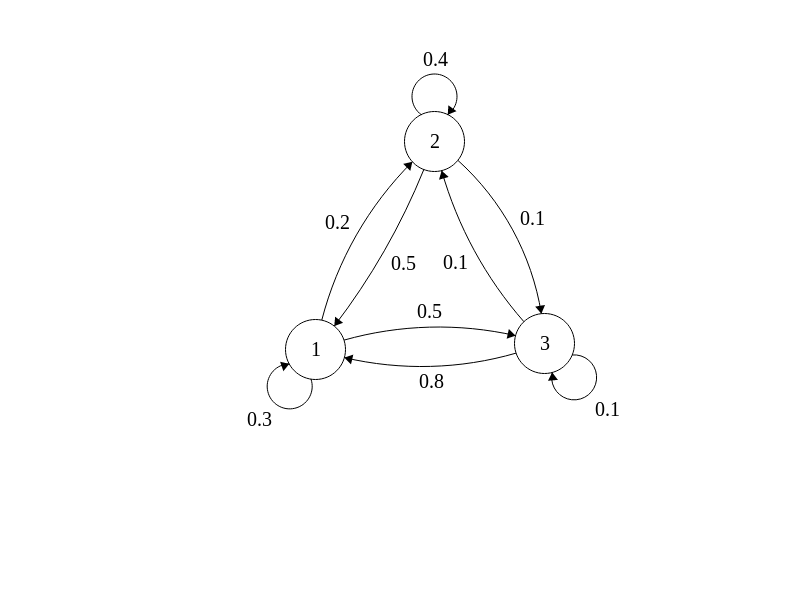
\includegraphics[scale=0.5,trim={0 5cm 0 1cm},clip]{figs/reinforcement_learning/mdp.png}
\caption{Markov Decision Process (MDP) with three states $\mathcal{S}=\{s_1,s_2,s_3\}$ and three possible actions $\mathcal{A}=\{a_1,a_2,a_3\}$, moving to state $s_1$, moving to state $s_2$ and moving to state $s_3$.}
\label{fig:MDP}
\end{figure}

Consider the (simplified) MDP represented in Figure \ref{fig:MDP}: it consists of three states $(s_1, s_2,\text{ and }s_3)$ that are connected by three actions (move to state $s_1, s_2,\text{ or }s_3$). 
For the MDP represented above we define the state transition probability matrix $\mathcal{P}^a_{ss'}=p(S_{t+1}=s'\mid S_{t}=s, A_t=a)$. In this MDP (our MDP is thus actually a Markov Reward Process (MRP) with deterministic state transitions), we assume that when we choose to move to state $s_i$, $i=\{1,2,3\}$ we always end up in that state, meaning that $\mathcal{P}^a_{ss'}=p(S_{t+1}=s'\mid S_{t}=s, A_t=a)=1$. In this case, $\mathcal{P}^{\pi}=\mathcal{P}^a_{ss'}\pi(a\mid s) = \pi(a\mid s)$. 
The rewards $\mathcal{R}_s^a$ are $[1.5, -1.8333 \text{ and } 19.8333]$ for a transition into state 1, 2, and 3, respectively. So, in our example $\mathcal{R}_s^a$ depends only on action (i.e. destination state) but it doesn't depend on source state.

We define as well the reward function over the policy $\pi$ as the expected reward considering all possible actions:
\begin{align*}
    {\mathcal{R}}^{\pi}(s) & = \sum_{a \in \mathcal{A}} \pi(a|s) \mathcal{R}_s^a
\end{align*}
We will use below expected values of the expected reward ${\mathcal{R}}^{\pi}(s)=[ 10.0, 2.0, \text{ and } 3.0 ] $ for state 1, 2, and 3, respectively.

\subsection{Policy Evaluation}
In the following exercises we will look at different ways of evaluating a given policy, meaning how to compute its value. 
 A central tool for this task is the \textbf{Bellman Expectation Equation}, which tells us how to decompose the state-value function into immediate reward plus discounted value of successor state:
\begin{align*}
    v_{\pi}(s) & = \mathbb{E}_{\pi}[R_{t+1} + \gamma v_{\pi}(S_{t+1}) | S_t = s]\\
    & = \sum_{a \in \mathcal{A}} \pi(a|s) \left( \mathcal{R}_s^a + \gamma \sum_{s' \in \mathcal{S}} \mathcal{P}_{ss'}^a v_{\pi}(s') \right).
\end{align*}

There are different ways of solving this problem. A straightforward solution is to solve the linear equation directly using linear programming:
\begin{align*}
    \boldsymbol{v}_{\pi} & = (\boldsymbol{I} -  \gamma \boldsymbol{\mathcal{P}}^{\pi})^{-1} \boldsymbol{\mathcal{R}}^{\pi}.
\end{align*}
However, this process involves the full knowledge of the transition function and requires a matrix inversion operation, which augments any errors coming from an approximate estimate of the transition probabilities.
Additionally, because of the complexity of matrix inversion, this solution is applicable only to small MDPs. For larger MDPs, we can use the \textbf{iterative policy evaluation} algorithm using the Bellman Expectation Equation.

\begin{exercise}
\label{exercise:PolicyEvaluation}
Implement policy evaluation by dynamic programming and linear programming. Check that you obtain the same value.

\begin{python}
import numpy as np

policy=np.array([[0.3, 0.2, 0.5], [0.5, 0.4, 0.1], [0.8, 0.1, 0.1]])
# 'raw_rewards' variable contains rewards obtained after transition to each state
# In our example it doesn't depend on source state
raw_rewards = np.array([1.5, -1.833333333, 19.833333333])
# 'rewards' variable contains expected values of the next reward for each state
rewards = np.matmul(policy, raw_rewards)

state_value_function=np.array([0 for i in range(3)])

for i in range(20):
    print(state_value_function)
    state_value_function=# TODO: Implement the Policy Evaluation Update with a Discount Rate of 0.1
print(state_value_function)

solution=# TODO: Implement the linear programming solution
print(solution)
\end{python}
\end{exercise}

\section{Monte Carlo and Q-Learning Solutions}

While Dynamic Programming techniques allow to iteratively compute policy evaluation and optimization problems, a disadvantage of these techniques is the fact that we need to know a full MDP model (transition probabilities) and touch all transitions and rewards in learning. Monte Carlo techniques circumvent this problem by learning from episodes that are sampled under a given policy. An algorithm for \textbf{Monte Carlo Policy Evaluation} looks as follows: 
\begin{itemize}
  \item Sample episodes $S_0, A_0, R_1, \ldots, R_T \sim \pi$.
    \item For each sampled episode:
  \begin{itemize}
  \item Increment state counter $N(s) \leftarrow N(s) + 1$.
  \item Increment total return $S(s) \leftarrow S(s) + G_t$.
    \end{itemize}
  \item Estimate mean return $V(s) = S(s)/N(s)$.
  \end{itemize}

A more sophisticated technique is the so-called \textbf{Q-Learning} algorithm. In contrast to the simple Monte Carlo Policy Evaluation algorithm given above, it updates not towards the actual return $G_t$, but towards an estimate $(R_{t+1} + \gamma \max_{a'} Q(S_{t+1},a')$ (the so-called Temporal Difference (TD) target). This replacement is also known as bootstrapping, where instead of computing the full return, we replace it with the estimate of the immediate reward and the value of the consecutive state. It thus combines Dynamic Programming (in form of the Bellman Optimality Equation) and Monte Carlo (by sampling episodes).

\begin{algorithm}[h!]
\label{algo:q-learning}
   \caption{Q-Learning}
\begin{algorithmic}[1]
\FOR{sampled episodes}
\STATE Initialize $S_t$
\FOR{steps $t$} 
\STATE Sample $A_t$, observe $R_{t+1}$, $S_{t+1}$.
\STATE $Q(S_t,A_t) \leftarrow (1 - \alpha) Q(S_t,A_t) + \alpha (R_{t+1} + \gamma \max_{a'} Q(S_{t+1},a'))$
\STATE $S_t \leftarrow S_{t+1}$.
\ENDFOR
	\ENDFOR
\end{algorithmic}
\end{algorithm}

\begin{exercise}
Implement Monte Carlo policy evaluation. See how similar results can be
obtained by using sampling
\begin{python}
import numpy as np

policy=np.array([[0.3, 0.2, 0.5], [0.5, 0.4, 0.1], [0.8, 0.1, 0.1]])
rewards=np.array([10., 2., 3.])

import random
from collections import defaultdict
reward_counter=np.array([0., 0., 0.])
visit_counter=np.array([0., 0., 0.])

def gt(rewardlist, gamma=0.1):
    '''
    Function to calculate the total discounted reward
    >>> gt([10, 2, 3], gamma=0.1)
    10.23
    '''
    #TODO: Implement the total discounted reward
    return 0

for i in range(400):
    start_state=random.randint(0, 2)
    next_state=start_state
    rewardlist=[]
    occurence=defaultdict(list) 
    for i in range(250):
        rewardlist.append(rewards[next_state]) 
        occurence[next_state].append(len(rewardlist)-1) 
        action=np.random.choice(np.arange(0, 3), p=policy[next_state]) 
        next_state=action

    for state in occurence: 
        for value in occurence[state]: 
            rew=gt(rewardlist[value:]) 
            reward_counter[state]+=rew 
            visit_counter[state]+=1 
            #break #if break: return following only the first visit

print(reward_counter/visit_counter)
\end{python}

Implement Q-Learning policy optimization in a simple exercise. This samples a state-action pair randomly, so that all the state-action pairs can be seen.
\begin{python}
q_table=np.zeros((3, 3)) 
for i in range(1001): 
    state=random.randint(0, 2) 
    action=random.randint(0, 2) 
    next_state=action
    reward=rewards[next_state] 
    next_q=max(q_table[next_state])
    q_table[state, action]= #TODO: Implement the Q-Table update
    if i%100==0:
        print(q_table)
\end{python}
\end{exercise}


\section{Policy Gradient Techniques}

The Dynamic Programming and Monte Carlo techniques discussed above can be summarized under the header of \emph{value-based} techniques since they focus on how to obtain the optimal policy by first computing the value functions. They are thus inherently indirect, which brings forth different problems, such as they are very sensitive to errors in the estimation of the value function.
 Direct solutions to policy optimization exist and avoid this caveat. Some approaches resort to gradient-based techniques to optimize parametric (stochastic) policies, and are called \emph{policy gradient} techniques. Given an action-value function $q_{\pi_\theta}(S_t,A_t)$, the objective is to maximize the expected value  \[\max_{\theta} \mathbb{E}_{\pi_{\theta}}[q_{\pi_\theta}(S_t,A_t)].\]
The gradient of this objective takes a very useful form:
\[\mathbb{E}_{\pi_{\theta}}[q_{\pi_\theta}(S_t,A_t) \nabla_{\theta} \log \pi_{\theta}(A_t|S_t)].\]
It can be though of as the expectation of the gradient of the score function weighted by its value.
The well-known REINFORCE algorithm optimizes this objective by using stochastic gradient ascent updates and by replacing $q_{\pi_\theta}(S_t,A_t)$ by the actual return $G_t$.

\begin{algorithm}[h!]
\label{algo:reinforce}
   \caption{REINFORCE}
\begin{algorithmic}[1]
\FOR{sampled episodes $y=S_0, A_0, R_1, \ldots, R_T \sim \pi_\theta$}
\FOR{time steps $t$} 
\STATE Obtain reward $G_t$%$q_{\pi_\theta}(S_t,A_t)$
\STATE Update $\theta \leftarrow \theta + \alpha (
G_t
%q_{\pi_\theta}(S_t,A_t) 
\nabla_{\theta} \log \pi_{\theta}(A_t|S_t))$
\ENDFOR
	\ENDFOR
\end{algorithmic}
\end{algorithm}



\begin{exercise}
Implement the score function gradient estimator in lxmls/reinforcement\_learning/score\_function\_estimator.py. Check it is correct by calling the train() function.
\begin{python}
% matplotlib inline
from lxmls.reinforcement_learning.score_function_estimator import train
train()
\end{python}
\end{exercise}

Now you can apply REINFORCE to a simulated agent task, the cart pole task: A pole is attached by an un-actuated joint to a cart, which moves along a frictionless track. The system is controlled by applying a force of +1 or -1 to the cart, which results in the cart moving forward or backwards respectively. The pole starts upright, and the goal is to prevent it from falling over. A reward of +1 is provided for every timestep that the pole remains upright. The episode ends when the pole is more than 15 degrees from vertical, or the cart moves more than 2.4 units from the center. See \url{ https://gym.openai.com/envs/CartPole-v1/}.

\begin{exercise}
Implement policy gradient for the cartpole task by coding the forward pass of Model() in lxmls/reinforcement\_learning/policy\_gradient.py. Check it is correct by calling the train() function.
\begin{python}
from lxmls.reinforcement_learning.policy_gradient import train
train()
\end{python}
\end{exercise}


\begin{exercise}
As a last exercise, apply what you have learned to the RNN model seen in previous days. Implement REINFORCE to replace the maximum likelihood loss used on the RNN day. For this you can modify the PolicyRNN class in lxmls/deep\_learning/pytorch\_models/rnn.py 
\begin{python}
# Load Part-of-Speech data 
from lxmls.readers.pos_corpus import PostagCorpusData
data = PostagCorpusData()

# Get batch iterators for train and test
batch_size = 1
train_batches = data.batches('train', batch_size=batch_size)
dev_set = data.batches('dev', batch_size=batch_size)
test_set = data.batches('test', batch_size=batch_size)
\end{python}
\begin{python}
reinforce = True

# Load version of the RNN 
from lxmls.deep_learning.pytorch_models.rnn import PolicyRNN
model = PolicyRNN(
    input_size=data.input_size,
    embedding_size=50,
    hidden_size=100,
    output_size=data.output_size,
    learning_rate=0.05,
    gamma=0.8,
    RL=reinforce,
    maxL=data.maxL
)
\end{python}

After finishing the implementation, the following code should run
\begin{python}
import numpy as np
import time

# Run training
num_epochs = 15

batch_size = 1
# Get batch iterators for train and test
train_batches = data.sample('train', batch_size=batch_size)
dev_set = data.sample('dev', batch_size=batch_size)
test_set = data.sample('test', batch_size=batch_size)

# Epoch loop
start = time.time()
for epoch in range(num_epochs):
    # Batch loop
    for batch in train_batches:
        model.update(input=batch['input'], output=batch['output'])
    # Evaluation dev
    is_hit = []
    for batch in dev_set:
        loss = model.predict_loss(batch['input'], batch['output'])
        is_hit.extend(loss)
    accuracy = 100 * np.mean(is_hit)
    # Inform user
    print("Epoch %d: dev accuracy %2.2f %%" % (epoch + 1, accuracy))

print("Training took %2.2f seconds per epoch" % ((time.time() - start) / num_epochs))
# Evaluation test
is_hit = []
for batch in test_set:
    is_hit.extend(model.predict_loss(batch['input'],batch['output']))
accuracy = 100 * np.mean(is_hit)

# Inform user
print("Test accuracy %2.2f %%" % accuracy)
\end{python}
\end{exercise}


% \appendix

% \chapter{Installation Guide}
% \input{pages/appendix/installation}
% \chapter{Data Sets}
% \input{pages/appendix/data-sets}


%\bibliographystyle{plain}
\bibliographystyle{apalike}
\bibliography{guide}
\end{document}
%%% Local Variables: 
%%% mode: latex
%%% TeX-master: t
%%% End: 
